% =====================================================================================================
% vygotskian_machine.tex — The Vygotskian machine, part 1: the framing section
%
% DRAFT (2026-11-19). Opens the three-part proposal; a proposal, not a report of results.
% Include from main.tex, in this order:
%     % =====================================================================================================
% vygotskian_machine.tex — The Vygotskian machine, part 1: the framing section
%
% DRAFT (2026-11-19). Opens the three-part proposal; a proposal, not a report of results.
% Include from main.tex, in this order:
%     % =====================================================================================================
% vygotskian_machine.tex — The Vygotskian machine, part 1: the framing section
%
% DRAFT (2026-11-19). Opens the three-part proposal; a proposal, not a report of results.
% Include from main.tex, in this order:
%     % =====================================================================================================
% vygotskian_machine.tex — The Vygotskian machine, part 1: the framing section
%
% DRAFT (2026-11-19). Opens the three-part proposal; a proposal, not a report of results.
% Include from main.tex, in this order:
%     \input{vygotskian_machine}
%     \input{vygotskian_cortex}
%     \input{vygotskian_internalisation}
%     \input{vygotskian_cultural_plane}
%     \input{vygotskian_experiments}
% with \addbibresource{vygotskian_machine.bib} and \usepackage{array} in the preamble.
% =====================================================================================================

\section{The Vygotskian Machine}
\label{sec:vygotskian}

According to Vygotsky, higher mental functions develop in accordance with one central law: each function first
emerges in interactions between people, and then within the individual \cite{vygotsky1978mind}. A child plans aloud
together with an adult before planning aloud alone, plans aloud alone before planning silently, and plans silently
before the plan is carried out without any words at all. Language is what carries the child through this sequence. It
is the means by which knowledge held by other people becomes the learner's own, and it is also the tool with which the
learner regulates its own actions while that knowledge is still new.

We propose to build a robot that follows this law, and we call it a \emph{Vygotskian machine}. The robot's higher
functions, such as its goals, its plans, the meaning it gives to a scene and what it expects to find in a room, are
first provided from outside. They come from the person who lives with the robot and from a vision-language model (VLM),
a neural network trained on images and text that carries a large share of human culture. The robot then internalises
these functions, first as an inner voice that asks questions, makes plans and imagines outcomes
(Section~\ref{sec:inner_speech}), and eventually as prior beliefs, accumulated counts of experience and habits that
need no language at all. The robot's automatic level consists of the Active Inference agents that build its hierarchy
of beliefs and control its movement. This automatic level is what the internalised knowledge ultimately shapes, and
it is also the level that language is called upon to assist whenever the situation exceeds its competence.

\begin{table}[ht]
    \centering
    \small
    \begin{tabular}{|>{\raggedright\arraybackslash}p{0.4\linewidth}|>{\raggedright\arraybackslash}p{0.5\linewidth}|}
        \hline
        \textbf{Vygotsky} & \textbf{The machine} \\ \hline
        Every higher function emerges first between people, and then within the individual
            & goals, plans and scene meaning arrive as a person's words and the VLM's culture, then become priors,
              plans and habits (Sections~\ref{sec:lang_hierarchy:culture}--\ref{sec:lang_hierarchy:sequencing}) \\ \hline
        Outer speech $\to$ private speech $\to$ inner speech $\to$ no speech
            & the VLM writes a mission; the inner voice rehearses and monitors it; the compiled habit runs without
              language (Eq.~\ref{eq:lh_habit}) \\ \hline
        Private speech rises with task difficulty and fades with mastery \cite{berk1992children}
            & the demand signal recruits the voice on surprise and leaves it idle when the automatic level copes
              (Section~\ref{sec:inner_speech:modes}) \\ \hline
        Scaffolding by a more knowledgeable other, withdrawn as competence grows \cite{wood1976role}
            & the VLM's prior weight is overtaken by the robot's own counts (Eq.~\ref{eq:lh_beta_prior}); the person
              is asked less as experience accumulates \\ \hline
        The zone of proximal development: what the learner can do only with help
            & situations outside the automatic level's competence but within reach with the VLM or the person;
              learning moves them inside \\ \hline
        Mediation by signs: language as a psychological tool
            & the VLM's output is never accepted as belief; instead, it structures what the robot's own models do by
              proposing, sequencing and choosing what to imagine (Table~\ref{tab:lh_roles}) \\ \hline
    \end{tabular}
    \caption{Vygotsky's account and its counterpart in the proposed machine.}
    \label{tab:vygotskian_mapping}
\end{table}

\paragraph{Internalisation in Active Inference.}
Within the framework of this document, the passage from outer to inner speech can be given a precise
interpretation. Culture enters the generative model, the robot's probabilistic model of how its observations are
produced, in two places. It enters as prior beliefs and preferences, which describe what a room is for, which objects
tend to appear together and which outcomes are acceptable, and it enters as candidate policies, that is, sequences of
actions, which are scored by their expected free energy. Experience then internalises this culture in the two
corresponding places. The priors are progressively replaced by counts of what the robot itself has observed, and the
candidate policies that continue to succeed become part of the habit prior, a learned preference over policies. The
machine's dependence on language for routine matters should therefore decrease with experience, while remaining for
situations that are novel, social or structural.

\paragraph{Organisation.}
Section~\ref{sec:cortex} describes CORTEX, the architecture on which the machine is built. CORTEX already includes a
language agent, and the machine is defined by what it adds to that architecture. Section~\ref{sec:inner_speech}
develops internalisation. It treats the inner voice as an epistemic action, that is, an action taken to gain
information, and describes the attention modes that call on the voice and release it, as well as the learning that the
voice drives. Section~\ref{sec:lang_hierarchy} develops the cultural plane. It explains how the VLM is connected to the
belief hierarchy in three roles, namely culture, sequencing and imagination, under the rule that the language model
proposes and the generative models dispose.

\paragraph{The internalist contrast.}
According to the opposing, internalist view, language evolved first as an internal system for thought and was only
later used to communicate \cite{berwick2016why}. We use this view as a contrast rather than as a rival, because the
distinction it draws between the faculty of language and the content that language carries
(Section~\ref{sec:inner_speech:why_lm}) is what makes the Vygotskian claim testable. A machine that has a
compositional inner language but no culture serves as the \emph{non-Vygotskian control}. Its inner language is built
by library learning, the gradual collection of reusable sub-programmes, from the robot's own experience alone
(Section~\ref{sec:inner_speech:library}). If this control machine performs as well as the machine fed with culture in
situations far from anything the robot has seen, then culture is not doing the work that the name of the machine
claims for it.

\paragraph{Prior uses of the idea.}
Mirolli and Parisi argued for a Vygotskian cognitive robotics in which language serves as a cognitive tool as well as
a means of communication \cite{mirolli2011towards}, and Colas et al.\ proposed Vygotskian autotelic agents that
internalise language and culture to imagine and pursue their own goals \cite{colas2022language}. The present proposal
shares their premise but differs from them in three respects. First, internalisation is formalised within Active
Inference, as culture that enters priors and policies and gradually settles into counts and habits. Second, the
internalised knowledge acts on a probabilistic belief hierarchy whose evidence rules and cavity messages, which exclude
a belief's own contribution from the evidence it receives, prevent the hierarchy from confirming itself. Third, an
attention mechanism decides, from moment to moment, whether language is needed at all.

\paragraph{Two bitter lessons.}
Any proposal that builds knowledge into a robot has to respond to what Sutton called the bitter lesson. According to
Sutton, across seventy years of AI research, general methods that scale with computation, search and learning have
eventually outperformed methods that build in what their designers know \cite{sutton2019bitter}. Chess programs built
on human expertise were overtaken by search, and speech and vision systems built on expert-designed features were
overtaken by statistical learning. A robot whose levels 1 to 3 are generative models written by its designers, and
whose prior about kitchens is a table of log-odds written by hand, is open to the same criticism. A second lesson has
recently been drawn from the success of the first. Verbelen argues that ``the main idea behind modern AI is not
learning. It is amortisation'' \cite{verbelen2026newbitter}. In this view, training converts expensive inference into
reusable structure, so that a foundation model is a store of distilled past computation. Amortisation works when the
future resembles the past and fails when it does not. From this follows the new bitter lesson, that ``intelligence
cannot be fully amortised''. A system that must face a changing world needs, in addition to what it has precomputed,
three capabilities that amortisation does not supply, namely learning online during deployment, exploring actively to
reduce its own uncertainty, and forming new hypotheses when the old model no longer fits.

\paragraph{Where the Vygotskian machine stands.}
The two lessons pull in opposite directions. The first advises against handcrafting knowledge and in favour of using
what large-scale training has learned. The second warns that what large-scale training has learned is not enough, and
that a system must continue to perform inference. Neither lesson says how a system should combine the two, and such a
combination is what the Vygotskian machine proposes. Its novelty lies in four aspects.

\begin{enumerate}[(i)]
    \item \emph{Amortised culture as a proposal, never as a belief.} The VLM is the most amortised object
    available, since it contains human culture distilled by training at scale. The machine treats it as exactly
    that, the product of a general method, and uses it where Sutton's lesson says such methods should be used,
    namely to replace the hand-written parts of the system. The authored log-odds of the kitchen prior become priors
    elicited from the VLM, and the meaning of a room, which no designer has written down, also comes from the VLM.
    The machine never uses the VLM's output as its belief. Instead, the VLM's proposals are scored by ongoing
    inference against evidence, including evidence that something is absent, and they enter the generative model as
    pseudo-counts, imaginary prior observations that the robot's own experience gradually outweighs
    (Eq.~\eqref{eq:lh_beta_prior}).
    \item \emph{Internalisation is amortisation by the robot, with a way back.} The robot amortises its own
    ongoing inference, in the sense that what the inner voice works out in focused mode settles into priors, counts
    and habits that no longer need language. This process is the internalisation described by Vygotsky's law, and it
    is also the amortisation of the second lesson, carried out by the agent itself, on its own data, while it acts.
    Each compiled habit carries with it the assumptions under which it was learned
    (Section~\ref{sec:lang_hierarchy:sequencing}). When the probability of those assumptions falls, the habit is set
    aside and ongoing inference takes over again.
    \item \emph{A signal that decides when amortisation is enough.} The new bitter lesson states that
    amortisation fails when the situation is novel, but it does not say how an agent notices that this has happened.
    In the machine, this decision is made continuously by a demand signal, which is a prediction error weighted by
    its precision, that is, by the confidence placed in it (Section~\ref{sec:inner_speech:modes}). While the amortised
    levels predict well, the inner voice either remains silent or imagines, and a surprise calls on ongoing inference
    mediated by language. Private speech in children behaves in the same way, increasing with task difficulty and
    fading as the child gains mastery.
    \item \emph{The three missing properties, each with its own mechanism.} Online learning consists of the
    gradual replacement of the VLM's pseudo-counts by experience and the growth of the habit prior with experience.
    Active exploration takes the form of the inner question, treated as an epistemic action and scored by its
    expected information gain (Section~\ref{sec:inner_speech:questions}). New hypotheses arise from surprise at the
    level of the model itself. When the evidence for an arrangement of objects collapses, or when a class of objects
    repeatedly fails to fit where it is expected, the VLM proposes a new structure and the robot's own models test
    it. In every case, the VLM generates candidates and the robot's models evaluate them.
\end{enumerate}

The machine thus interprets the first lesson as a reason to take culture from a learned model instead of writing it
by hand, and the second as a reason to keep that culture outside the belief state, where ongoing inference can correct
it. Vygotsky's account supplies the developmental sequence that connects the two lessons, in which knowledge is first
borrowed from others, then used through speech, and finally internalised until it no longer needs speech.

\paragraph{What would demonstrate that the paper's goal has been achieved?}
The central claim rests on three predictions. First, the non-Vygotskian control falls behind the machine fed with
culture in proportion to the novelty of a situation (P7 in Section~\ref{sec:inner_speech:predictions}). Second, the
machine's use of language behaves as private speech does, increasing with difficulty and decreasing with mastery
(P8). Third, the scaffold provided by the VLM is withdrawn, so that as confirmed rooms and successful missions
accumulate, the number of calls to the VLM falls while task success is maintained (L6 in
Section~\ref{sec:lang_hierarchy:predictions}).

%     % =====================================================================================================
% vygotskian_cortex.tex — The Vygotskian machine, part 2: the CORTEX architecture it is built on
%
% DRAFT (2026-11-20, cut to budget). Describes what exists today, as a given resource. Descriptive, not a report
% of results: every component named here is in the robocomp/active_inference repository (ARCHITECTURE.md is the
% source). Include after vygotskian_machine.tex and before vygotskian_internalisation.tex.
% =====================================================================================================

\section{The Starting Point: the CORTEX Architecture}
\label{sec:cortex}

The Vygotskian machine is added to an existing and working robot architecture, \cortex{}, which runs on a mobile
robot called Shadow, both in a simulated apartment and in a real one. \cortex{} already builds a probabilistic model of
the robot's surroundings, acts on that model, remembers it, and talks about it with a person
through a language agent. We describe the architecture as it stands, because each proposal in the later sections is
defined by what it adds to these parts.

\input{figures/cortex-architecture-overview}

\paragraph{A shared graph of beliefs.}
At its core, \cortex{} is a shared, distributed and persistent scene graph, read and written concurrently by independent
processes called agents (Figure~\ref{fig:cortex_overview}, where the graph is drawn as the working memory). Agents
do not send messages to one another, and the graph
is the only interface through which they communicate. Each agent keeps a full replica, and the replicas are merged as
conflict-free replicated data types, whose copies converge to the same state without coordination. Geometric edges
hold a rigid transform with its covariance, and they form a tree from the world through the rooms to the objects, and
from the robot's base to its sensors. An agent is a process that maintains a probabilistic belief over one kind of
entity and publishes it with its mean and covariance. Other agents treat this posterior as evidence weighted by its
covariance, and never as ground truth. Effects that a conventional system would express as a threshold, such as
ignoring distant detections, are instead written into the generative model, usually as a covariance that grows with a
physical quantity. The thresholds that this paper does introduce are declared, with their justification, in
Section~\ref{sec:inner_speech:modes}.

\paragraph{A probabilistic hierarchy.}
The beliefs in the graph form a hierarchy of five levels (Table~\ref{tab:lh_levels}), namely the robot itself, its
rooms, the objects in those rooms, aggregates of objects, and cultural abstractions such as what a room is for. Each
level is expressed in the frame of the level below, its measurements are the posteriors published by that level, and
it can send back down an empirical prior, that is, a message stating what it expects its parts to be. The first four
levels constitute \cortex{} as it exists, and they are built automatically and without language. The fifth is the
addition made in this paper. Figure~\ref{fig:cortex_graph} shows the graph that \cortex{} builds in the simulated
apartment.

\begin{table}[ht]
    \centering
    \small
    \begin{tabular}{|>{\raggedright\arraybackslash}p{0.05\linewidth}|>{\raggedright\arraybackslash}p{0.16\linewidth}|>{\raggedright\arraybackslash}p{0.33\linewidth}|>{\raggedright\arraybackslash}p{0.17\linewidth}|>{\raggedright\arraybackslash}p{0.13\linewidth}|}
        \hline
        \textbf{Level} & \textbf{What} & \textbf{Latent} & \textbf{Source of its model} & \textbf{Status} \\ \hline
        0 & robot (self) & body, sensor mounts, pose & calibration, self-calibration & implemented \\ \hline
        1 & room(s) & layout of each room, the robot's place in it, the doors that join rooms & authored generative model, fitted online; spatial memory & implemented \\ \hline
        2 & objects & per instance: class, pose, extent, existence & authored generative models, fitted online & implemented \\ \hline
        3 & metaconcepts (aggregates) & arrangements: a ring of chairs around a table, the rectilinear frame of a kitchen & authored schemas & implemented (the kitchen's priors not yet sent down) \\ \hline
        4 & cultural abstraction & the function of a room (kitchen, dining, bedroom, \ldots) & \textbf{culture: the VLM}, weighted by measured reliability and replaced by counts & \textbf{added by this paper} (Section~\ref{sec:lang_hierarchy:culture}) \\ \hline
    \end{tabular}
    \caption{The probabilistic belief hierarchy. Levels 0--3 are \cortex{} as it exists, and level 4 is added here.}
    \label{tab:lh_levels}
\end{table}



\paragraph{Levels 0 to 3.}
At level 0, an agent dedicated to the body maintains the tree of frames from the base to each sensor, and a
self-calibration agent estimates where each sensor is mounted, so that these transforms are themselves beliefs. At
level 1, a room agent jointly estimates the layout of the current room and the robot's location in it, and decides
from evidence whether the robot has entered a new room or returned to a known one. Rooms are joined by doors, and the
robot's world is a graph of rooms of which only one is actively estimated at a time. At level 2, each class of object
has its own concept agent, for tables, chairs, cabinets, refrigerators, doors, beds, people and others. Each agent
tracks instances from segmentation masks and depth, updates a class-specific generative model with a shared recursive
variational Laplace engine, and publishes each instance in the frame of its room. A residual agent models the
occupancy that no other agent explains, and acts as the null hypothesis of the scene. Every instance carries an
existence log-odds, raised by evidence that was predicted and observed and lowered by evidence that was predicted but
absent, only where the object could have been detected, so that an occluded object is retained rather than refuted.
At level 3, two metaconcepts fit aggregates, a table with its ring of chairs and the frame shared by the units of a
kitchen. The existence of an aggregate is a log Bayes factor against an explicit null of independent objects, and
each aggregate sends empirical priors to its members, computed without that member's own contribution
(Eq.~\eqref{eq:lh_cavity}). Level 4, the purpose of a room and how the robot should behave there, is not represented
in \cortex{} and is the contribution of this paper (Section~\ref{sec:lang_hierarchy:culture}).



\begin{figure}[!h]
    \centering
    \begin{minipage}[c]{0.53\linewidth}
        \centering
        \begin{tikzpicture}
            \node[anchor=south west, inner sep=0] (img) at (0,0)
                {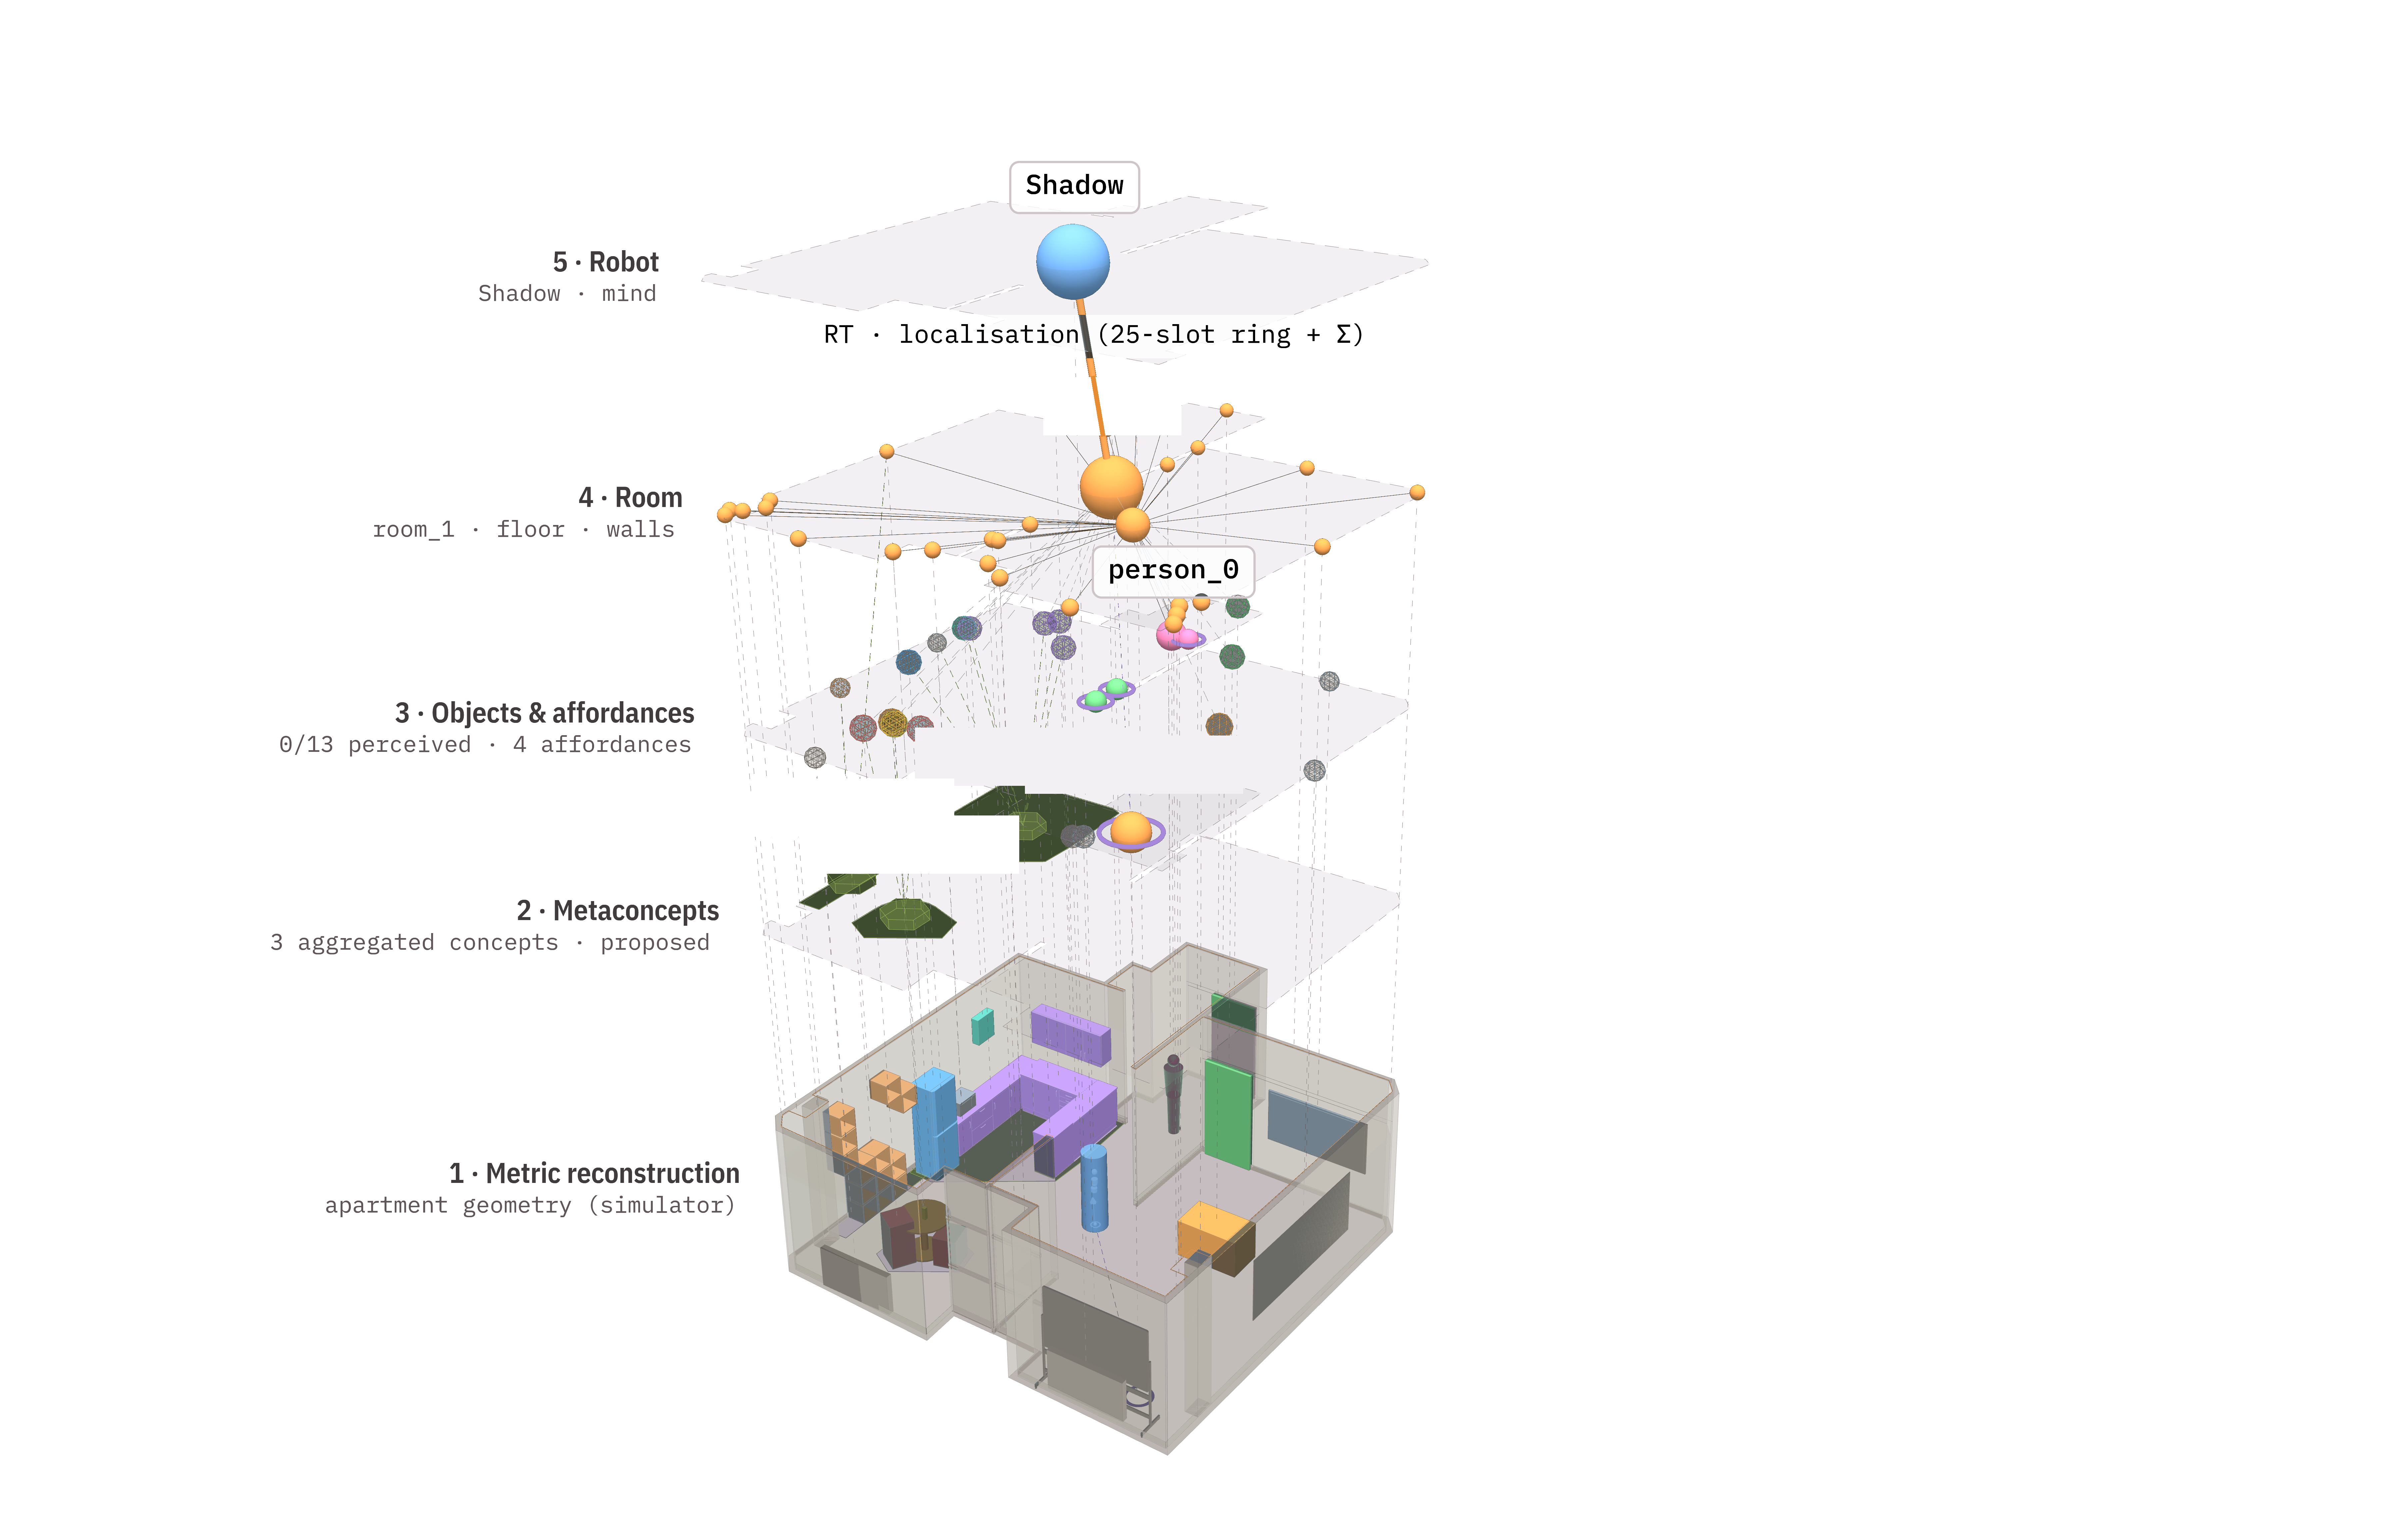
\includegraphics[width=\linewidth,trim=760 200 2850 420,clip]{figures/full_graph_white_clean.png}};
            \begin{scope}[x={(img.south east)}, y={(img.north west)}]
                % labels redrawn apart; the overlapping originals were removed from full_graph_white_clean.png
                \tikzset{lab/.style={draw=black!45, fill=white, rounded corners=1.5pt, inner sep=1.2pt,
                         font=\ttfamily\tiny}}
                \node[lab, anchor=east] at (0.690,0.800) {room\_1};
                \node[lab, anchor=west] at (0.425,0.505) {wall-shelf};
                \node[lab, anchor=west] at (0.470,0.462) {dinner-set};
                \node[lab, anchor=west] at (0.565,0.542) {kitchen-rig};
                \node[lab, anchor=west] at (0.775,0.515) {afford\_room};
                \fill[yellow!85!orange, draw=conceptc!80!black, thick] (0.80,0.585) circle (2.6pt);
                \node[draw=black!50, fill=white, rounded corners=1.5pt, inner sep=1.5pt,
                      font=\ttfamily\tiny, anchor=west] at (0.825,0.60) {chair\_34};
            \end{scope}
        \end{tikzpicture}
    \end{minipage}\hfill
    \begin{minipage}[c]{0.43\linewidth}
        \centering
        \resizebox{\linewidth}{!}{\input{figures/belief-node}}
    \end{minipage}
    \caption{Left: the output of \cortex{} in the simulated apartment, drawn by stratum: the robot (level~0),
    localised in \texttt{room\_1} (level~1); the objects and their affordances (level~2); and the aggregates fitted
    over them (level~3). The bottom stratum is the simulator's true geometry, shown for reference, and strata numbers
    give the drawing order, not the levels of Table~\ref{tab:lh_levels}. Right: a schematic of the node marked \texttt{chair\_34} on the left, as a belief
    owned by one agent, whose existence log-odds rises when the object is seen, is held while it is occluded, and
    falls only when it is absent where it could have been detected.}
    \label{fig:cortex_graph}
\end{figure}

\paragraph{Action and memory.}
A controller plans and follows paths. Its epistemic planner scores the actions that the concept agents offer, such as
looking at a door from a given place, by their expected free energy. An exploration drive turns this scoring into a
default behaviour. The robot explores the current room until further exploration yields too little information,
crosses the nearest uncrossed door, and returns in depth-first order. Three memory agents retain what the live graph
discards. The spatial memory stores each room the robot has left with the doors that connect it, and restores it as a
prior on return. The object memory keeps a persistent record of object instances. The episodic memory records the
robot's missions, their steps and how each ended. These memories provide the counts from which the priors and habits
of the Vygotskian machine will be learned.

\paragraph{The language agent.}
The language agent connects a person to all of these components through a vision-language model (VLM), Gemma 4
with 26 billion parameters, served by Ollama on an NVIDIA Jetson AGX Orin carried by the robot. Its design follows the principle
stated in the code as ``the model proposes, C++ decides''. The VLM sees a summary of the graph and the memories and can
act only by calling tools, and every call passes a deterministic gate that checks names against the graph and
arguments against the robot's capabilities. Extended behaviour is written in a small mission language (cross a door,
explore a room, approach an object, watch for a condition, if, repeat), and each mission is checked against the graph
and approved by the person before it runs. While a mission runs, robot events wake the model in restricted turns in
which it can look, query memory, stop and propose, but not act. Whether to ask the person or to make an assumption is
decided by a small rule over counts and costs. The agent also answers subjunctive questions with the robot's own
models, on an imagined copy of the room that can never write to the live graph. On that copy the controller answers
``would I fit?'', the perception models answer ``would I see it from there?'', and the episodic counts answer ``would
this route succeed?''. The imagination of Section~\ref{sec:lang_hierarchy:imagination} relies on these tools.

\paragraph{What is missing.}
\cortex{} can therefore perceive, hold beliefs, act, remember, talk and, when asked, imagine. Its VLM is used only when a
person speaks, nothing it knows becomes a prior, the robot never questions itself or imagines on its own initiative,
and the hundredth mission to the kitchen requires the same VLM calls as the first. The inner voice
(Section~\ref{sec:inner_speech}) and the cultural plane (Section~\ref{sec:lang_hierarchy}) address these gaps.

%     % =====================================================================================================
% vygotskian_internalisation.tex — The Vygotskian machine, part 2: internalisation (the inner voice)
%
% DRAFT (2026-11-19; first drafted 2026-11-18 as inner_speech_section.tex). A proposal section: it describes an
% architecture that is NOT yet implemented, grounded in the existing language_agent (robocomp/active_inference).
% Include from main.tex, in this order:
%     \input{vygotskian_machine}
%     \input{vygotskian_internalisation}
%     \input{vygotskian_cultural_plane}
% and add the shared bibliography:  \addbibresource{vygotskian_machine.bib}
% Packages used: amsmath, amssymb, enumitem (already loaded by main.tex) and array, which main.tex does not
% load yet: add \usepackage{array} to its preamble.
% Labels keep their original sec:inner_speech:* prefix so that existing cross-references do not break.
% =====================================================================================================

\section{Internalisation: the Inner Voice}
\label{sec:inner_speech}

The robot described so far uses language in one direction only: a person speaks, and a language agent turns
the request into commands for the controller, grounded in a textual digest of the belief graph. This section
proposes to turn that capability inward, which constitutes the internalisation step of the Vygotskian machine
(Section~\ref{sec:vygotskian}). We argue that a language model embedded in an Active Inference
architecture can play the role that inner speech plays in human cognition, namely that of a serial and
compositional medium in which the agent poses questions to itself, generates hypotheses, rehearses plans and
replays its past. We further argue that this role follows naturally from the epistemic component of expected free
energy. The proposal is presented together with the constraints that prevent such a voice from becoming a source
of confabulated beliefs, and with the experiments that would falsify it.

\subsection{Motivation: from talk to thought}
\label{sec:inner_speech:motivation}

Two theoretical traditions disagree about the origin of inner speech, but they agree about its function. According
to the developmental view that gives the machine its name, inner speech is social speech that the child gradually internalises, abbreviates and
turns into a tool for self-regulation \cite{vygotsky1986thought}. According to the internalist view, which we use
as the point of contrast throughout this section, human language evolved first as an internal system for structuring thought, and its use for
communication is a later externalisation \cite{berwick2016why}. Contemporary reviews treat inner speech as
functionally involved in planning, problem solving, self-monitoring and the maintenance of goals in working memory
\cite{aldersonday2015inner}, and language more generally as a cognitive technology that lets a learner manipulate
discrete, recombinable tokens rather than raw percepts \cite{clark1998magic}.

Large language models provide a striking example of the developmental route. They are trained exclusively on
communicative text, yet their performance improves measurably when they produce intermediate reasoning in that
same medium before answering, a technique known as chain-of-thought \cite{wei2022chain}. In this sense, a system
built for communication becomes better at reasoning when it addresses its speech to itself. Our language agent is
at a comparable point in its own development. It was built to converse with a person, and the question we ask is
what it contributes once its speech is addressed to the robot itself.
Section~\ref{sec:inner_speech:why_lm} returns to the internalist contrast, and Section~\ref{sec:inner_speech:library}
turns it into a control experiment.

\subsection{Inner questions as epistemic actions}
\label{sec:inner_speech:questions}

In Active Inference, policies are scored by expected free energy, whose epistemic term rewards the expected
reduction of uncertainty about hidden states \cite{friston2017process, parr2022active}. A question can be
regarded as the linguistic expression of exactly this quantity, since it names a hidden variable whose value is
uncertain and whose resolution is expected to matter. We therefore model an inner question as a persistent object
\begin{equation}
    \mathcal{Q} = \big\langle\, e,\; \mathcal{H},\; q(h),\; \mathcal{P},\; b,\; s \,\big\rangle ,
    \label{eq:inner_question}
\end{equation}
where $e$ is the triggering event (for example an obstacle no concept agent explains), $\mathcal{H}$ a finite set
of named hypotheses (``a chair'', ``a box'', ``unknown''), $q(h)$ the current posterior over them, $\mathcal{P}$
the set of pending predictions, $b$ a budget in time and motion, and $s \in \{\text{open},\text{resolved},
\text{abandoned}\}$ its status. Questions are organised as a stack, in the sense of a \emph{question under
discussion} \cite{roberts2012information}, so that ``is it a chair?'' is a sub-question whose answer partially
resolves the parent question ``what is this?''. It is the question object, and not the language model's context
window, that carries the state of the reasoning from one step to the next.

\paragraph{One step of the loop.}
Given $\mathcal{Q}$, the language model proposes a test, which consists of an epistemic action $a$ (turning
towards the anomaly, approaching it, looking with the front camera) together with the outcome that each hypothesis
predicts. The value of the test
is its expected information gain minus its cost,
\begin{equation}
    V(a) \;=\; \underbrace{H\!\left[q(h)\right] \;-\; \mathbb{E}_{p(o \mid a)}\!\left[ H\!\left[q(h \mid o, a)\right]
    \right]}_{I(h;\,o \mid a)} \;-\; c(a),
    \label{eq:inner_value}
\end{equation}
which is the negative of the epistemic part of expected free energy with an explicit action cost. The test is
executed only if $V(a) > 0$ and the action passes the same deterministic gate that already validates every
command the language agent issues. When the observation $o$ arrives, the posterior is updated by the concept
agents' own likelihoods,
\begin{equation}
    q(h \mid o, a) \;\propto\; p(o \mid h, a)\, q(h),
    \label{eq:inner_update}
\end{equation}
and the loop continues, spawns a sub-question, or terminates when
\begin{equation}
    H\!\left[q(h)\right] < \eta \quad\lor\quad \max_a V(a) \le 0 \quad\lor\quad b \text{ exhausted}.
    \label{eq:inner_stop}
\end{equation}
This stopping rule is what distinguishes reasoning from rumination. A loop with no expected information left to
gain is closed, possibly with the answer ``unknown'', and the event that triggered it is habituated, that is,
ignored for a refractory period.

\paragraph{The grounding constraint.}
The central design rule is that the language model may suggest hypotheses but only perception may decide between
them; in short, \emph{the language model proposes and perception disposes}. Text produced by the model may
introduce hypotheses, predictions and tests, but it may never change a posterior. Only the likelihood
$p(o \mid h, a)$ in \eqref{eq:inner_update}, computed by the perceptual agents from sensor data, can do so. This
rule is the counterpart, on the side of beliefs, of the rule that the language agent already enforces for actions,
under which every proposed command is validated in C++ against the belief graph before it reaches the controller.
Without it, a language loop addressed to itself would be a closed system in which text is conditioned only on
text, and it would converge on its own confabulations.

\paragraph{The proposer as a calibrated prior.}
The hypotheses the model names, and the probabilities it attaches to them, encode world knowledge the robot has
not acquired by itself (``chairs come with tables''). We treat this knowledge as a prior whose weight must be
earned through demonstrated accuracy. Let
$\pi_{\text{LM}}(h \mid x)$ be the proposer's distribution in context $x$ and $n_x(h)$ the robot's own counts of
resolved questions in that context. The prior entering \eqref{eq:inner_update} is
\begin{equation}
    q_0(h \mid x) \;\propto\; \pi_{\text{LM}}(h \mid x)^{\beta_x}\, \big(\alpha + n_x(h)\big),
    \label{eq:inner_prior}
\end{equation}
a tempered product of the proposer and a Dirichlet over experience, where $\beta_x \in [0,1]$ is set from the
proposer's measured calibration in that context (for instance from its Brier score on past questions). Early in
the robot's life the proposer dominates this prior, and as the counts accumulate, the robot's own experience
progressively replaces the knowledge borrowed from the language model. The same conjugate form already governs the language agent's decision to ask a person or to assume
that they moved an object, where a Beta posterior over the person's past answers is compared against the costs of
asking and of being wrong.

\subsection{Attention, automaticity and the wandering mind}
\label{sec:inner_speech:modes}

A human driver on an easy road can steer without attending to the road, which leaves the mind free to plan, imagine
or recall, and attention returns to the task as soon as something unexpected happens
\cite{smallwood2015science, christoff2016mind}. In Active Inference this phenomenon is described in terms of
precision. While prediction errors are small and the habitual policy is reliable, attention, understood as the
precision assigned to sensory prediction errors, can be withdrawn from the task, and a surprise raises it again
\cite{feldman2010attention}. The account in which habitual and deliberative control are arbitrated according to
their relative uncertainty \cite{daw2005uncertainty} has the same structure.

The architecture already separates the two systems. The controller and the concept agents form an automatic layer
that drives, avoids obstacles and executes missions without the language model, while the language agent provides
the deliberative voice. We propose to make the allocation of this voice explicit through a scalar \emph{demand}
signal, computed without the language model each time the textual digest of the belief graph is updated,
\begin{equation}
    D_t \;=\; \sum_{k} \pi_k\, \varepsilon_{k,t}^{2} \;+\; \lambda\, \mathbb{1}\!\left[\text{person active}_t\right],
    \label{eq:inner_demand}
\end{equation}
where $\varepsilon_{k,t}$ are normalised prediction errors reported by the agents (unexplained residual occupancy,
flips of existence or door beliefs, localisation uncertainty, stalled or failed mission steps, controller refusals)
and $\pi_k$ their precisions. Three operating modes then follow from two thresholds with asymmetric hysteresis:
\begin{equation}
    m_t =
    \begin{cases}
        \textsc{focused}    & D_t > \theta_{\text{hi}},\\[2pt]
        \textsc{wandering}  & D_\tau < \theta_{\text{lo}} \;\; \forall\, \tau \in [t - T, t],\\[2pt]
        \textsc{monitoring} & \text{otherwise.}
    \end{cases}
    \label{eq:inner_modes}
\end{equation}
Entering \textsc{wandering} requires demand to stay low for a dwell time $T$; leaving it requires a single sample
above $\theta_{\text{hi}}$. The robot is therefore slow to let its attention drift away from the task and
immediate in returning to it. Safety never depends on this arbitration, because the controller's reflexes act on
their own and the deliberative voice engages only after the reflex has acted, just as a driver becomes aware of a
hazard only after having braked.

\paragraph{Focused mode} runs the question loop of Section~\ref{sec:inner_speech:questions} on the triggering
event. \paragraph{Monitoring mode} makes no calls to the language model, so that the voice is ready to engage but
remains silent.

\paragraph{Wandering mode.}
When the voice is freed from the task, it is seeded with one recent experience chosen by salience, such as an
episode that ended unresolved, a failure, an object that changed, or an upcoming goal. The output of each step,
together with an associative retrieval from episodic memory, seeds the next step, so that the chain of thoughts
drifts in the way spontaneous thought does \cite{christoff2016mind}. The voice has access only to memory queries and to the architecture's imagination tools,
which simulate observations and outcomes on a copy of the belief graph; it can neither act nor write beliefs. Its
products are of three kinds: counterfactuals over past episodes (``had the door been open, the crossing would have
taken 40\,s less''), hypotheses to be tested later, and prospective plans (``if the door is shut on the way back,
the route through the next room is shorter''). Functionally, this corresponds to the role of the brain's default
network in simulating the past and the future \cite{buckner2008brain}, and to the offline replay and model reduction that Active Inference assigns
to rest and sleep \cite{friston2017curiosity, hobson2012waking}. Replay is prioritised by the expected gain of the
memory it revisits \cite{mattar2018prioritized}.

\paragraph{Source monitoring.}
Humans occasionally misremember imagined events as perceived ones \cite{johnson1993source}, and the robot must not
make this error.
Everything produced while wandering is stored with an \emph{imagined} provenance, separate from the factual
episodic record, and enters the learning loop only as a hypothesis to be tested, never as evidence.

\subsection{What the return to reality gives the automatic layer}
\label{sec:inner_speech:return}

The transition from \textsc{wandering} to \textsc{focused} cancels the chain of thought in progress (its state is
kept, so that it may resume if demand subsides) and devotes the voice entirely to the surprising event. This return
to reality serves the automatic layer on three timescales.
\begin{enumerate}
    \item \textbf{Decision.} A surprise indicates that the automatic layer has left its domain of competence, and
    outside that domain its only responses are to retry, to stop or to fail. The voice adds the re-interpretation of
    the scene, arbitration between goals, re-planning through the remembered topology, and recourse to a person.
    \item \textbf{Attention.} The voice can raise precision where it matters, by orienting sensors, increasing a
    detector's rate in a region, or passing a hypothesis to the concept agents as a spatial prior. Such a prior has
    bounded weight, so that it may accelerate the recognition of an object that is present but cannot create one
    that is absent, which preserves the grounding constraint.
    \item \textbf{Teaching.} Each resolved surprise is a labelled example that the automatic layer could not have
    produced alone. For instance, an unexplained residual later identified as a chair is a false negative of the
    chair detector, a door that is repeatedly shut in the evening becomes a prior, and a recovery that repeatedly
    succeeds becomes a branch of the controller's behaviour tree. In this way the domain of competence grows and the
    situations that require the voice become rarer, which is the classical progression from effortful to autonomous
    skill \cite{fitts1967human}.
\end{enumerate}
Plans prepared while wandering act as a store of precomputed solutions, so that when the anticipated situation
occurs, the focused voice verifies an existing plan instead of composing a new one. The return ends with an
explicit release, in which spatial priors are cleared, safety margins are restored and the automatic layer is
confirmed to be back within its competence. Without this release, every surprise would leave the robot permanently
vigilant.

\subsection{Relation to chain-of-thought reasoning}
\label{sec:inner_speech:cot}

Chain-of-thought reasoning is a form of inner speech in the functional sense, although of a specific kind, and
comparing the two clarifies the design (Table~\ref{tab:inner_cot}). Plain chain-of-thought is convergent and
ungrounded, in that each token is conditioned only on previous tokens until an answer is produced, after which the
trace is discarded. Reasoning becomes grounded when it is interleaved with action and observation
\cite{yao2023react}. Our focused loop is of this kind, with the additional property that the observation, through
\eqref{eq:inner_update}, rather than the next token, determines the direction the reasoning takes. The wandering
voice is closer to plain chain-of-thought in its isolation from perception, but it is divergent rather than
convergent, it can be interrupted, and its products persist.

\begin{table}[ht]
    \centering
    \small
    \begin{tabular}{|>{\raggedright\arraybackslash}p{0.19\linewidth}|>{\raggedright\arraybackslash}p{0.22\linewidth}|>{\raggedright\arraybackslash}p{0.24\linewidth}|>{\raggedright\arraybackslash}p{0.24\linewidth}|}
        \hline
                                & \textbf{Chain-of-thought} & \textbf{Focused voice} & \textbf{Wandering voice} \\ \hline
        Goal                    & answer a given question   & resolve a given surprise & none given; seeded by salience \\ \hline
        Dynamics                & convergent                & convergent             & divergent, associative \\ \hline
        Contact with the world  & none                      & thought--action--observation & none (imagination only) \\ \hline
        Persistence             & discarded                 & question objects, beliefs, lessons & imagined store, hypotheses \\ \hline
        Interruptible           & no                        & yes                    & yes, resumable \\ \hline
        Latency budget          & n/a                       & $\sim$1\,s, no extended thinking & unbounded, extended thinking \\ \hline
    \end{tabular}
    \caption{Chain-of-thought compared with the two modes of the proposed inner voice.}
    \label{tab:inner_cot}
\end{table}

Two practical consequences follow. First, extended reasoning should take place \emph{when there is time, not when
there is pressure}. In the deployed language agent the model's extended thinking is disabled, because a model
operating in thinking mode spent 3\,000--6\,000 tokens (40--80\,s) before each tool call. Such a delay is
incompatible with the focused mode but costs nothing in the wandering mode, where extended thinking can be enabled
with a large budget and pre-empted at any moment. In this way slow reasoning is carried out in advance, and fast
reasoning makes use of its results. Second, chain-of-thought traces are known not always to reflect the
computation that produced the answer \cite{turpin2023language}, as human verbal reports do not always reflect the
causes of behaviour \cite{nisbett1977telling}. The faithful record of the robot's reasoning is therefore the
structured record of hypotheses, predictions, observations and posterior updates, not the generated text. Finally,
wandering chains whose hypotheses were later confirmed by perception form a corpus of reasoning verified against the world,
which could be used to fine-tune the local model in the manner of self-taught reasoning \cite{zelikman2022star},
with perception, rather than a known answer, as the filter.

\subsection{Consequences for belief and learning}
\label{sec:inner_speech:learning}

The question loop changes the way beliefs evolve in two respects. Within an episode, uncertainty is reduced where surprise
occurred rather than where the sensors happened to point, which is efficient but leaves the rest of the map less
examined and makes the robot's own data a biased sample; a decaying novelty term \cite{schwartenbeck2019curiosity}
and importance weighting of learned statistics are required to correct this. Across episodes, every closed
question is a labelled example, and learning proceeds at four timescales (Table~\ref{tab:inner_learning}).

\begin{table}[ht]
    \centering
    \small
    \begin{tabular}{|>{\raggedright\arraybackslash}p{0.14\linewidth}|>{\raggedright\arraybackslash}p{0.37\linewidth}|>{\raggedright\arraybackslash}p{0.37\linewidth}|}
        \hline
        \textbf{Timescale} & \textbf{What changes} & \textbf{Where, in this architecture} \\ \hline
        Seconds   & posterior over the hypotheses of one question         & the question object \eqref{eq:inner_question} \\ \hline
        Days      & priors: where objects are, which doors are shut, what moves & long-term object and topological memory, as Dirichlet counts \\ \hline
        Weeks     & likelihoods: detector and concept models              & false negatives and positives labelled by resolved questions \\ \hline
        Slow      & structure: new categories                             & recurrent, mutually similar ``unknown'' resolutions named by the voice and proposed as a new concept \\ \hline
    \end{tabular}
    \caption{Learning driven by the inner-question loop.}
    \label{tab:inner_learning}
\end{table}

The last row of the table engages most directly the hypothesis that language serves as a medium for thought,
since a cluster of anomalies that no existing concept can explain becomes learnable once it has been named. The
loop also learns about its own operation. The salience weights $\pi_k$ in \eqref{eq:inner_demand} are adjusted
according to the information that each trigger actually yielded, the option of asking a person is weighed against
that of looking, and loops that repeatedly resolve the same way are compiled into
reflexive rules, so that the number of language-model calls per hour should \emph{decrease} as competence grows.

\subsection{Why a language model: generation versus evaluation}
\label{sec:inner_speech:why_lm}

Since none of the above requires a person, it is natural to ask what a language model contributes to an
architecture that already performs inference and action selection. Our answer rests on a division of labour. Expected
free energy evaluates policies and Bayesian updating weighs hypotheses, but both operate over a space that has
already been enumerated: each concept agent carries a fixed generative model, policies must be listed before they
can be scored, and Bayesian model reduction can prune structure but not invent it \cite{friston2017curiosity}.
Whatever falls outside the given models remains an unexplained residual. A language model is weak where this
machinery is strong, since its confidences are not calibrated posteriors and it has no access to the sensors, and
it is strong where this machinery is weak, since it is an inexpensive and broad generator of hypotheses,
explanations and plans. We therefore use it only as a \emph{proposal distribution}, that is, as a source of
candidates in a generate-and-test loop whose test is carried out by active inference:
\begin{itemize}
    \item \emph{Hypotheses outside the built-in models.} A residual blob can be proposed to be a bag, a toppled
    chair or a robot vacuum, none of which any concept agent represents; the question loop then tests them.
    \item \emph{Amortised policy search.} Instead of enumerating multi-step policies, the model writes a few
    candidate missions, which are small programs in the mission language; the gate validates them and expected
    free energy scores them.
    \item \emph{Relational binding across agents.} The agents' representations (signed distance fields, occupancy
    grids, existence log-odds, episodic records) are mutually incompatible, whereas a sentence such as ``the chair
    that was not next to the table in the room behind door~3 yesterday'' binds them in a single query that no
    individual agent could formulate.
    \item \emph{Explanation from few examples.} After a single surprise the model can propose which variable
    mattered (``the door is shut because it is evening''), turning one episode into a testable generalisation.
    \item \emph{Abstraction and naming.} Episodes are compressed into reusable lessons, and recurrent unknowns are
    named, which is what makes them candidates for a new concept (Table~\ref{tab:inner_learning}).
\end{itemize}
The use of language, rather than an arbitrary learned embedding, matters for three reasons. Language is discrete
and compositional, so that new hypotheses and plans can be assembled from known parts; it is inspectable, so that
deterministic gates can parse and check it and people can audit it; and, once the robot thinks in it,
communication with a person comes at no further cost.

\paragraph{Where the knowledge comes from.}
This argument raises a difficulty for the internalist thesis introduced in the motivation. If the inner voice
precedes the outer one, the common-sense knowledge on which the value of the proposer rests cannot have arrived
through communication, and yet a language model acquires all of that knowledge from human text, that is, from the
outer voices of other people. The difficulty disappears once the language \emph{faculty} is distinguished from its
\emph{content}. The internalist claim concerns the former, namely a computational system for building unbounded
hierarchical structures, which is available for thought before it is used for communication
\cite{hauser2002faculty, berwick2016why}. It makes no claim that what a person knows was acquired without
language. Human knowledge has three sources: core systems for objects, agents, number and space, present before
learning \cite{spelke2007core}; individual experience; and, once outer language exists, cumulative cultural
transmission, which supplies most of what an adult knows \cite{tomasello1999cultural}. Even on the internalist
view, the inner voice of a modern human is filled largely by the outer voices of others.

The architecture has the same three sources of knowledge, arranged differently. The hand-built generative models
of the concept agents play the role of \emph{core knowledge}, since they are given before experience and limited
to a few domains. The robot's own counts $n_x(h)$ in \eqref{eq:inner_prior} constitute \emph{individual
experience}. The language model plays the role of \emph{culture}, that is, of knowledge distilled from a
community's communication and inherited by this individual at birth. The robot therefore resembles a child born
into a culture more than an early hominin, and its inner voice is Vygotskian in origin, because both its format and
its content were learned from outer speech. Two consequences follow. First, the proposal does not demonstrate the
internalist thesis and should not be read as doing so. Its claim is functional, namely that an inner use of
language has epistemic value independently of communication, and this claim holds whatever the origin of the
language system. Second, the format and the content of the voice can in principle be separated, which turns the
question into an experiment. A compositional generator over the robot's own concepts and mission language, trained
only on the robot's experience, would supply the format without the culture. Section~\ref{sec:inner_speech:library}
describes such a generator.

\subsection{A control experiment: a language-like format without human culture}
\label{sec:inner_speech:library}

We claim that a Vygotskian machine needs culture and not merely a language-like format, and this claim can be
tested only against a machine that has the format without the culture. Library learning, a technique from the
field of program induction, offers a concrete candidate for such a machine. DreamCoder \cite{ellis2021dreamcoder} learns to
solve tasks by writing programs and, at the same time, learns the language in which it writes them. It maintains a
library $\mathcal{L}$, initially a small base language of typed primitives, and a prior $P(\rho \mid \mathcal{L})$
over programs $\rho$ given by a probabilistic grammar over that library, under which a program that reuses library
functions is short and therefore probable. Each task $x$ supplies a likelihood $P(x \mid \rho)$, in the original
work usually the indicator that $\rho$ solves $x$. The system seeks the library and the sets of solutions
$\mathcal{F}_x$ that jointly maximise
\begin{equation}
    P(\mathcal{L}) \prod_{x \in \mathcal{X}} \sum_{\rho \in \mathcal{F}_x} P(x \mid \rho)\, P(\rho \mid \mathcal{L}),
    \label{eq:dc_objective}
\end{equation}
together with a recognition model $Q(\rho \mid x)$, a neural network that predicts from a task which parts of the
library its solution is likely to use. Optimisation alternates three phases:
\begin{enumerate}
    \item \textbf{Wake.} For each task, programs are enumerated in decreasing probability under $Q$, within a time
    budget, and the best few that solve it are kept in $\mathcal{F}_x$.
    \item \textbf{Abstraction sleep.} The solutions found so far are refactored to expose shared sub-programs, and
    those whose addition to $\mathcal{L}$ most shortens the library plus the rewritten solutions become new library
    functions, following a minimum description length criterion. Refactoring by inverse $\beta$-reduction over
    version spaces finds abstractions that appear in no program literally.
    \item \textbf{Dream sleep.} $Q$ is trained to minimise $-\log Q(\rho \mid x)$ on two sources: \emph{replays}, the
    tasks solved in wake paired with their solutions, and \emph{fantasies}, programs sampled from the current
    library and executed to produce synthetic tasks, as in the Helmholtz machine \cite{dayan1995helmholtz}.
\end{enumerate}
The three phases reinforce one another, because a richer library makes complex solutions short, short solutions
are found sooner, more solved tasks provide more material to compress, and a better recognition model makes the
search faster. Concepts such as higher-order list functions or parametrised drawing routines appear in the library
without ever being defined by hand. Later work makes abstraction learning substantially faster
\cite{bowers2023stitch} and uses a language model to guide the search and to name the learned abstractions
\cite{grand2024lilo}, but this use of a language model reintroduces precisely the culture that the present
experiment excludes.

\paragraph{Relation to the inner voice and to free energy.}
The negative logarithm of \eqref{eq:dc_objective} is a description length: the complexity of the library and the
programs plus the inaccuracy of the programs on the tasks. Its minimisation is therefore a form of free-energy
minimisation over structure, and abstraction sleep is the constructive counterpart of the Bayesian model reduction
that Active Inference assigns to sleep \cite{friston2017curiosity}. Whereas reduction removes structure whose
complexity is not justified by the accuracy it provides, abstraction adds structure whose complexity is justified
in this way. The three phases also correspond to the modes of
Section~\ref{sec:inner_speech:modes}. Wake is the focused voice solving questions and carrying out missions;
abstraction sleep is consolidation while wandering, which compresses repeated solutions into reusable lessons; and
dream sleep is imagination while wandering, which trains the proposer on simulated outcomes. In this generator the
recognition model occupies the place that the language model occupies in Section~\ref{sec:inner_speech:why_lm},
since it is also a learned proposal distribution, but one trained only on what this robot has done and imagined.

\paragraph{Two ways to apply library learning to the robot.}
\begin{itemize}
    \item \emph{Over the mission language, for policies.} The base language is the mission language's operations
    (\texttt{cross}, \texttt{explore}, \texttt{approach}, \texttt{watch}, \texttt{if}, \texttt{repeat}) and its
    predicates. Tasks are the goals the robot has been given or has set itself through inner questions, and the
    likelihood is the probability that a mission achieves its goal, measured by the controller's outcome on the
    real robot or, cheaply and repeatably, in simulation. The learned library entries are macro-missions, such as
    ``look behind door~$D$ and return'' or ``approach $X$ from the side it was last seen from'', which are
    discovered by compressing the robot's own successful missions instead of being written by people.
    \item \emph{Over shape primitives, for new concepts.} The concept agents already describe object classes as
    compositions of primitives in signed distance fields; a table, for instance, is a smooth box top on four
    cylindrical legs. Taking these primitives and their composition operators (smooth union, placement, repetition,
    symmetry) as the base language, a recurrent cluster of residual observations that every concept agent leaves
    unexplained becomes a task, which consists of finding a program whose distance field explains the point clouds
    of the clusters. The
    likelihood is the concept agents' existing measurement model, a noise model on signed distance, and the
    continuous parameters of each candidate program are fitted with the same optimisers the concept agents use.
    Compression across clusters yields reusable parts and whole-object programs, and a program that recurs is a
    candidate for a new concept agent. This is structure learning whose candidates come from perception rather than
    from text.
\end{itemize}

\paragraph{How the robot setting differs from program induction.}
Applying library learning to the robot requires three departures from the original setting. First, likelihoods are graded and noisy rather than binary, which
the objective \eqref{eq:dc_objective} admits directly but which makes enumeration less decisive. Second, real tasks
are expensive, since a mission takes minutes and a cluster accumulates over days, so that dream sleep in simulation
carries more of the learning than it does in DreamCoder. Third, tasks are few, so the inner question loop also
serves as a curriculum, in which surprises select the tasks on which the library is trained.

The resulting library is a compositional language of thought whose vocabulary comes only from what the robot has
perceived and done. Its abstractions are unnamed, because naming them requires a language shared with others. It
is at this point that a language model, and with it culture, would enter the architecture, in order to externalise
concepts that already exist internally, which is the order that the internalist thesis proposes.

\subsection{Mapping onto the existing architecture}
\label{sec:inner_speech:mapping}

Several components already exist in the language agent (Section~\ref{sec:cortex}). Robot events (mission reports, failures, completions)
already activate the model through a queue, in turns during which the model may perceive, query memory, stop and
propose, but never act. Every action already passes a deterministic validation gate. The decision whether to ask a
person or to make an assumption is already taken on decision-theoretic grounds. Unexplained occupancy is already isolated by a residual agent that acts as the null
hypothesis of the scene, and the episodic and long-term object memories can already be queried jointly in
read-only mode. The components still missing are the persistent question objects \eqref{eq:inner_question}, a prediction evaluator implementing
\eqref{eq:inner_update} outside the language model, the demand signal and mode arbitration
\eqref{eq:inner_demand}--\eqref{eq:inner_modes}, the imagined store with its provenance, and the channel through
which bounded spatial priors reach the concept agents.

\subsection{Testable predictions}
\label{sec:inner_speech:predictions}

In keeping with the evaluation principle adopted throughout this paper, under which policies are compared against
each other inside one closed loop with the body, sensors and environment held fixed, the proposal makes eight
falsifiable predictions, each tested in simulation by moving known objects and introducing unfamiliar ones:
\begin{enumerate}[label=\textbf{P\arabic*}]
    \item The unexplained residual mass per room decreases faster with the focused loop than without it.
    \item The proposer's calibration on resolved questions improves, and $\beta_x$ in \eqref{eq:inner_prior}
    decreases, as the robot's own counts accumulate.
    \item Detector false-negative rates fall after retraining on question-labelled examples.
    \item Inner questions per hour decrease over repeated exposure to the same environment while answer accuracy
    is maintained.
    \item Plans prepared while wandering reduce the latency from surprise to a validated response, and the time to
    notice a deliberately moved object does not grow despite habituation.
    \item With the language-model proposer replaced by a fixed hypothesis set (the existing concept classes and
    ``unknown'') and template-based missions, the loop resolves fewer questions about objects and failures outside
    the built-in models, and acquires new categories more slowly.
    \item \emph{The non-Vygotskian control.} A library-learning generator trained only on the robot's own experience
    (Section~\ref{sec:inner_speech:library}), with no language model in the loop, supplies the format without the
    culture. The prediction has two parts.
    \begin{enumerate}[label=(\alph*)]
        \item \emph{Policies.} Over the mission language, the mean description length of the robot's successful
        missions decreases across wake--sleep cycles; the library-learning proposer approaches the language-model
        proposer on recurring goal types in a familiar environment, and falls further behind it the further a goal
        departs from those seen before.
        \item \emph{Concepts.} An object class absent from every concept agent and introduced in simulation (boxes,
        for instance) is recovered as a library program whose likelihood on held-out instances exceeds that of the
        ``unknown'' model, and whose adoption as a concept prior reduces the unexplained residual mass.
    \end{enumerate}
    \item \emph{Private speech.} The rate of language-model calls behaves as children's private speech does
    \cite{berk1992children}: within an environment it rises when tasks are made harder or novel (doors shut that are
    usually open, unfamiliar objects introduced) and falls with repeated exposure to the same tasks, while task
    success is maintained.
\end{enumerate}
A failure of P1 would indicate that the epistemic value of language-mediated questions does not exceed that of
the existing exploration; a failure of P4 would indicate that the loop does not transfer competence to the
automatic layer, which is its principal claim; and a failure of P6 would indicate that the language model adds
nothing a fixed hypothesis set does not, which would remove the case for including it. P7 is the control for the
central claim of the machine, because it separates the contribution of language as a format for thought from that
of the culture it carries. If the culture-free generator matches the culture-fed one on situations far from the robot's
experience, the machine need not be Vygotskian; if it falls behind there, culture is doing work that format alone
cannot. Success of P7(b) would in addition show that a compositional inner language grounded only in perception can
form a new concept before any word for it exists. P8 tests the dynamics implied by the name of the machine, in
which language is recruited when a task becomes difficult and withdrawn once the task has been mastered.

\subsection{Limitations}
\label{sec:inner_speech:limitations}

The demand signal \eqref{eq:inner_demand} sums heterogeneous prediction errors whose precisions must themselves be
calibrated, and a poorly scaled term will either suppress the voice or keep it permanently engaged. A single
language model serves the person, the focused loop and the wandering loop; pre-emption keeps the person first but
bounds how much offline reasoning a busy robot can do. The tempered prior \eqref{eq:inner_prior} is a heuristic
combination rather than a derived posterior. The generator of P7 is substantially harder to build than the
ablation of P6. Library learning is computationally expensive, and its search over program structure must here be
interleaved with continuous fitting of shape parameters. Its base languages, namely the mission operations and the
shape primitives, are designed by people, so the generator is free of the culture carried by text but not of the
designers' knowledge, which plays the role of core knowledge. A cheaper approximation, in which a small pre-trained
model is fine-tuned on the robot's logs, would reintroduce culture through its pre-training. Finally, the analogy
with human inner speech is functional rather than mechanistic. The proposal is that the same computational role,
namely serial and compositional self-questioning in the service of epistemic value, is useful for a robot, not
that the robot's voice resembles the human one in any further respect.

%     % =====================================================================================================
% vygotskian_cultural_plane.tex — The Vygotskian machine, part 3: the cultural plane
%                                  (language over the belief hierarchy: culture, sequencing and imagination)
%
% DRAFT (2026-11-19; first drafted as language_hierarchy_section.tex). A proposal section: the architecture it
% describes is NOT yet implemented beyond the parts stated as existing. Source design note:
% docs/LANGUAGE_OVER_BELIEF_HIERARCHY.md.
% Include AFTER vygotskian_machine.tex and vygotskian_internalisation.tex (it refers to their equations and modes).
% Bibliography: vygotskian_machine.bib (shared). Packages: amsmath, amssymb, enumitem, array.
% friston2017deeptemporal duplicates main.tex's friston2017deep under a new key on purpose, so that this file builds
% with vygotskian_machine.bib alone; merge the two keys when the bibliographies are merged.
% Labels keep their original sec:lang_hierarchy:* prefix so that existing cross-references do not break.
% =====================================================================================================

\section{The Cultural Plane: Language over the Belief Hierarchy}
\label{sec:lang_hierarchy}

Section~\ref{sec:inner_speech} treated the language model as an inner voice and asked what language contributes to
thought. In this section we turn to the plane on which, according to Vygotsky, every higher function first appears,
namely the social and cultural plane (Section~\ref{sec:vygotskian}). The vision-language model (VLM) comes to the
robot already containing a large share of human common sense. For the robot, the VLM therefore plays the role of
\emph{culture}: it is an external store of knowledge that extends the robot's mind in the sense of
\cite{clark1998extended}, and the robot inherits this knowledge rather than acquiring it through its own experience
(Section~\ref{sec:inner_speech:why_lm}). The question we address is how such a store can be coupled to a belief state
that is built by probabilistic inference, in such a way that the robot benefits from the knowledge without also
inheriting the fact that the store is neither grounded in the robot's perception nor calibrated.

We propose to connect the VLM to the robot's \emph{belief hierarchy} in three roles, which we call culture,
sequencing and imagination. All three are governed by the same rule, which we state as \textbf{the language model
proposes, the generative models dispose}. The roles are arbitrated by the attention modes of
Section~\ref{sec:inner_speech:modes}, so that the VLM imagines while the automatic level runs well, and monitors and
replans when it does not.

\subsection{The automatic belief hierarchy}
\label{sec:lang_hierarchy:automatic}

The robot builds its belief state without language, using the probabilistic hierarchy of levels 0 to 3 described
in Section~\ref{sec:cortex} (Table~\ref{tab:lh_levels}). One property of that hierarchy is used repeatedly below. A
level-3 metaconcept sends each of its members an empirical prior computed from the arrangement fitted without that
member, which is the cavity distribution of expectation propagation \cite{minka2001expectation},
\begin{equation}
    q_{\setminus i}(\theta) \;\propto\; \frac{q(\theta)}{m_i(\theta)}.
    \label{eq:lh_cavity}
\end{equation}
Here $\theta$ are the parameters of the arrangement (for a kitchen, its axis, worktop height and carcass depth),
$q(\theta)$ is their posterior given all members, and $m_i(\theta)$ is the factor contributed by the posterior of
member $i$. This means that a member is never asked to agree with its own evidence. The hierarchy has three limits,
and the rest of the section addresses them. It cannot say what a room is \emph{for}, because the purpose of a room
is not a geometric fact. It cannot pursue a goal that it was not built to pursue. And it does not look ahead, because
its predictions concern the present scene rather than the outcome of what the robot is about to do.

\subsection{Three roles of the language model}
\label{sec:lang_hierarchy:roles}

\begin{table}[ht]
    \centering
    \small
    \begin{tabular}{|>{\raggedright\arraybackslash}p{0.14\linewidth}|>{\raggedright\arraybackslash}p{0.43\linewidth}|>{\raggedright\arraybackslash}p{0.33\linewidth}|}
        \hline
        \textbf{Role} & \textbf{What the VLM supplies} & \textbf{What decides} \\ \hline
        Culture     & priors and structure that the hierarchy cannot produce itself: room function, class co-occurrence, arrangement schemas, norms & evidence against a null hypothesis (the rules shared by all metaconcepts) \\ \hline
        Sequencing  & goals decomposed into missions over the hierarchy's beliefs, under contextual constraints, with the belief change each step should produce & a mission checker and command gate, the controller, then the belief dynamics \\ \hline
        Imagination & \emph{which} subjunctive questions to put to the robot's own models while the automatic level runs well & the models, run on an imagined copy of the world \\ \hline
    \end{tabular}
    \caption{The three roles. In each, the language model proposes and a generative model disposes.}
    \label{tab:lh_roles}
\end{table}

The three roles rest on the same asymmetry, which was already discussed in Section~\ref{sec:inner_speech:why_lm}.
Probabilistic inference evaluates hypotheses and policies well but cannot generate new ones, whereas a language model
generates them cheaply but cannot evaluate them. Each role therefore combines the two in a generate-and-test loop, in
which the language model generates candidates and the test is carried out by the robot's generative model.

\paragraph{The person is part of the scaffold.}
According to Vygotsky, the knowledge that is internalised comes from a more knowledgeable other, and the support this
other provides, known as scaffolding \cite{wood1976role}, is withdrawn as the learner's competence grows. The VLM is
one such other, since it makes culture available on demand. The person living with the robot is the second one, and
already plays this role in the deployed system. The person sets goals, answers the questions that the robot cannot
settle by looking, confirms a claim before it is stored, and approves a mission before it starts. In the cultural
plane, these answers are the most valuable evidence the robot receives. A room function confirmed by the person
contributes to the counts $n_f$ in \eqref{eq:lh_beta_prior}, and a plan that the person approved and that succeeded
contributes to the habit term $E$ in \eqref{eq:lh_habit}. The decision to ask the person rather than to look is
itself assigned a cost, as the language agent already does for objects that may have moved. Both forms of scaffolding
are designed to be withdrawn. The weight of the VLM decreases as the pseudo-count $\kappa\beta_f$ is outweighed by
experience, and the person is asked less often as the robot's own counts grow.

\subsection{Culture: a level-4 function hypothesis}
\label{sec:lang_hierarchy:culture}

\paragraph{Latent and evidence.}
For each room $r$ and function $f$ we maintain an independent hypothesis ``$r$ serves $f$'', which is compared with
the null hypothesis ``$r$ is a generic space''. The hypotheses are independent rather than mutually exclusive
categories, because open-plan rooms serve several functions, and because this is how the shared metaconcept
machinery already treats its instances. The evidence for a hypothesis comes from one observation model. For each
class $c$, the observation is a binary variable $z_c$ that equals one if $c$ has been detected in $r$, so that ten
chairs do not count as ten separate pieces of evidence. Under $f$, the class is present with probability
$\pi_{cf}$ and, if present, is detected with probability $d_c$, so that $P(z_c = 1 \mid f) = \pi_{cf} d_c$. Under
the null hypothesis the same holds with $\pi_{c0}$ in place of $\pi_{cf}$. The log-likelihood ratio of one class is
therefore $\log(\pi_{cf}/\pi_{c0})$ when it has been detected, and $\log\big((1 - \pi_{cf} d_c)/(1 - \pi_{c0}
d_c)\big)$ when it has not, and the detectability cancels from the first case. A detection may itself be false, so
we take the expectation of the log-ratio under the probability $p_c$ that the class has truly been detected,
\begin{equation}
    \Lambda_f(r) \;=\; \log\frac{P(f)}{P(0)} \;+\; \sum_c \Big[\, p_c \log\frac{\pi_{cf}}{\pi_{c0}}
    \;+\; (1 - p_c)\log\frac{1 - \pi_{cf}\, d_c}{1 - \pi_{c0}\, d_c} \Big],
    \qquad p_c = 1 - \prod_{i \in c} (1 - p_i).
    \label{eq:lh_function_evidence}
\end{equation}
Here $p_i$ is the existence probability of instance $i$ of class $c$ in $r$, the product runs over the instances
that have been observed at least once, and $p_c = 0$ for a class with no instance. The first term is the prior
log-odds of the function, which is elicited from the VLM together with $\pi_{cf}$. The probabilities $\pi_{c0}$ of
the null hypothesis are elicited in the same way, by asking the VLM about a generic room, and they are replaced by
the robot's counts over all the rooms it has confirmed. Put simply, a class that was found speaks for the functions
that expect it, and a class that was looked for and not found speaks against them in proportion to how thoroughly it
was looked for. When the presence of every class is certain, the sum is the exact log-likelihood ratio. When it is
not, the expectation of the log-ratio is an approximation to the log of the marginal likelihood, which we accept
because it keeps the contribution of each class separate.

Two dependences must be handled. First, the existence probability $p_i$ of an instance already depends on whether the
instance was seen again where it should have been, but it does not depend on the search for other instances of the
class. The detectability $d_c$ therefore enters the evidence once, through the second term. Second, several classes
are not independent given the function. A counter, a countertop, a hood and the cabinets of a kitchen occur together.
Classes that are members of a level-3 aggregate therefore contribute through the aggregate, as a single observation,
and not one by one. The dependence that remains between classes outside any aggregate makes $\Lambda_f$ somewhat
overconfident, and we list it among the limitations. At present $d_c$ is the room's exploration completeness
multiplied by a per-class detection rate. This scalar cannot register a search directed at a particular class, and
it must be replaced by a detectability model computed from the viewpoints the robot has actually occupied before the
second stage described below is enabled. The quantity $\Lambda_f(r)$ is the existence log-odds of the hypothesis,
and the birth and death of hypotheses follow the rules of the metaconcept machinery.

\paragraph{Priors from culture, replaced by experience.}
The conditional probabilities $\pi_{cf}$ cannot be supplied by any geometric model. We elicit them from the VLM over
a closed vocabulary, consisting of the class names already used in the graph and a fixed set of functions, and give
each of them a Beta prior whose strength must be earned through measured calibration,
\begin{equation}
    \pi_{cf} \sim \mathrm{Beta}\big(\alpha + \kappa\beta_f\,\pi^{\text{VLM}}_{cf},\;
    \alpha + \kappa\beta_f\,(1-\pi^{\text{VLM}}_{cf})\big),
    \qquad
    \hat\pi_{cf} = \frac{\alpha + \kappa\beta_f\,\pi^{\text{VLM}}_{cf} + n_{cf}}{2\alpha + \kappa\beta_f + n_f}.
    \label{eq:lh_beta_prior}
\end{equation}
Here $\alpha > 0$ is a small base count that keeps the prior defined when $\beta_f = 0$ and $n_f = 0$, and $\kappa$
is a small pseudo-count, chosen so that the VLM carries the weight of a few observed rooms rather than a hundred.
The factor $\beta_f \in [0,1]$ is the robot's estimate of the VLM's reliability for $f$, defined as in
\eqref{eq:inner_prior}. It is the posterior mean of a $\mathrm{Beta}(1,1)$ distribution over the probability that,
in a room whose function a person has stated, the hypothesis seeded by the VLM agrees with the person, and it is
updated only on such rooms, so that the VLM is never calibrated against labels that its own priors produced. The
count $n_f$ is the number of distinct rooms confirmed as serving $f$, and $n_{cf}$ is the number of those rooms that
contained $c$. A room counts once, however often it is visited. This is the same Dirichlet form as
\eqref{eq:inner_prior}, restricted to two outcomes. The effective weight of the VLM, $\kappa\beta_f/(\kappa\beta_f +
n_f)$, is large while few rooms have been confirmed and decreases as experience accumulates.

The counts must not be allowed to confirm the prior that produced them. If a room were counted because a posterior
computed with $\hat\pi_{cf}$ had become confident, and the classes it contained then increased $n_{cf}$, the VLM's
prior would confirm itself through the counts, without any new information entering. We therefore admit a room into
$n_f$ in one of two ways only. Either a person has stated its function, or the evidence \eqref{eq:lh_function_evidence}
for $f$ remains positive when it is recomputed with the VLM's pseudo-counts removed and with the room's own
contribution removed from the counts, that is, with a prior built only from the other rooms the robot has
confirmed. The second route is closed until a few rooms have been confirmed by a person. The same elicitation will
replace priors that are currently written by hand. For example, the class-membership
log-odds of the kitchen metaconcept are documented in its configuration as ``elicited, not measured'' and are still
awaiting a corpus from which to measure them.

\paragraph{How a function hypothesis influences lower levels without confirming itself.}
In the first stage, a function hypothesis sends nothing into the beliefs of its members. In the second stage it sends
only exploration targets, namely classes that are expected but not yet seen, each with a coarse placement. The
exploration drive and the next-best-view planners use these targets to value candidate viewpoints, and never treat
them as evidence that an object exists. This introduces a selection bias in where the robot looks, but it does not
contaminate the evidence, provided that the detectability in \eqref{eq:lh_function_evidence} is computed from the
viewpoints that the robot actually occupied, because absence is then counted only in the places that were searched. Only at a later stage, and only if its record justifies it, would a function seed
level-3 births, and in that case the down-date \eqref{eq:lh_cavity} would apply to the members it seeded, so that
an object born because ``kitchen'' predicted it is not counted as evidence for ``kitchen''. The cavity rule covers
only this route. It does not prevent self-confirmation through the counts of \eqref{eq:lh_beta_prior}, which is
prevented instead by the admission rule stated with that equation, and it does not protect against a VLM that is
wrong in the same way about every room, which only rooms confirmed by a person can reveal.

\paragraph{Norms.}
Each function also carries the contextual norms that the VLM supplies for it, such as moving quietly and slowly in a
bedroom at night, keeping clear of the work area in a kitchen that is in use, and never blocking a doorway. These
norms are not evidence. They are preferences of the generative model, and
Section~\ref{sec:lang_hierarchy:sequencing} uses them as planning constraints.

\paragraph{Model-level surprise.}
Levels 2--3 already produce signals indicating that their \emph{model} is wrong, as opposed to merely uncertain.
Such signals include an arrangement whose Bayes factor collapses, a member with a large cavity residual, a class that
persistently receives a membership score near zero, and two competing schemas that are both weak. These signals
trigger diagnosis in focused mode. An example from the live system illustrates this. A refrigerator received a
kitchen membership of $0.00$ because only base and wall units were modelled, so that its top, at $1.85$\,m, was
compared with a worktop plane at $0.90$\,m. A person diagnosed the structural defect, and adding a third, tall tier
to the model corrected it. In focused mode, the task of the VLM is to propose revisions of this kind, which change
the model itself rather than its parameters. For now, accepting such revisions remains the task of a person.

\subsection{Sequencing over the hierarchy}
\label{sec:lang_hierarchy:sequencing}

\paragraph{Goals at their own level.}
In the deployed system, mission predicates already refer to beliefs, for example a room explored with probability
$\geq 0.9$, a door open with probability $< 0.5$, or an object class that has been seen. The hierarchy extends the
vocabulary in which goals are stated and decomposed. This corresponds to the deep temporal structure of Active
Inference \cite{friston2017deeptemporal}, in which a goal is planned at its own level and then refined downward
(Table~\ref{tab:lh_goals}).

\begin{table}[ht]
    \centering
    \small
    \begin{tabular}{|>{\raggedright\arraybackslash}p{0.2\linewidth}|>{\raggedright\arraybackslash}p{0.27\linewidth}|>{\raggedright\arraybackslash}p{0.43\linewidth}|}
        \hline
        \textbf{Goal stated at} & \textbf{Example} & \textbf{Decomposition} \\ \hline
        Level 4, function    & ``go where people eat''           & room with the highest $\Lambda_{\text{dining}}$ $\to$ its dining set $\to$ a standpoint \\ \hline
        Level 3, aggregate   & ``check every chair at the table'' & the ring's members \emph{and its empty slots}, predicted but not yet seen \\ \hline
        Level 2, object      & ``approach the fridge''           & an approach to the object \\ \hline
        Level 1, room        & ``go to room 2''                   & the doors to cross, from the spatial memory of the rooms already visited \\ \hline
        Level 0, self        & ``turn 90 degrees''               & a relative motion \\ \hline
    \end{tabular}
    \caption{Goals are planned at their own level of the hierarchy and refined downward.}
    \label{tab:lh_goals}
\end{table}

\paragraph{Epistemic sequences.}
The exploration drive is the robot's compiled epistemic plan, that is, a fixed routine for gathering information, and
it is the right default for building the map. When the robot has a specific goal, however, the drive becomes
inefficient. To find a mug in a partly known house, the VLM writes a sequence that the drive cannot produce. The
robot goes to the room with the highest kitchen evidence (level 4), looks along the worktop plane where mugs are
usually placed (level 3), and approaches a mug once one is seen. The hierarchy indicates where the information is,
and the VLM determines the order in which to gather it and when to stop.

\paragraph{Every step predicts its belief outcome.}
At present, a mission step reports only completion or failure. We require each step also to declare the change in
belief that it should produce. A door crossing predicts that the robot's current room changes and that the new room
is recognised. An exploration step predicts that completeness rises and that some $\Lambda_f$ moves away from zero.
An approach predicts that the existence probability of the target stays high as the distance to it decreases. Let
$\phi_k$ be the predicate over beliefs that step $k$ predicts, which must hold by the end of the step, and let
$\psi_j$ be the assumptions on which the running plan relies (``door 3 is open'', ``room 2 is still the
kitchen''). Both enter the demand signal \eqref{eq:inner_demand} as surprisal terms,
\begin{equation}
    s^{\text{plan}}_t \;=\; -\log P_t(\phi_k) \;\;\text{at the step's deadline},
    \qquad
    s^{\text{assume}}_{j,t} \;=\; -\log P_t(\psi_j) \;\;\text{continuously},
    \label{eq:lh_plan_surprise}
\end{equation}
where $P_t$ is the current belief. The first term detects a step whose outcome diverged from its prediction even
though the step reported success. The second term raises attention when an assumption weakens, before any step has
failed, in the same way as a driver slows down on seeing a school sign rather than braking only when a child appears.
In either case, the focused voice replans from the belief state that the robot actually has. A plan thereby becomes
the same kind of object as an inner question (Section~\ref{sec:inner_speech:questions}), namely a proposal whose
predictions are confirmed or refuted by the belief dynamics.

\paragraph{Constraints from context.}
The norms attached to the active function hypotheses become invariants that apply to the whole mission, such as
avoiding a region, limiting the speed or keeping a distance. They are monitored for violation throughout the mission
rather than checked only once at its start.

\paragraph{Habits.}
Sequences that recur and succeed are compiled into habits. In Active Inference, the prior over policies combines a
habit term $E$ with the expected free energy $G$, weighted by a precision $\gamma$
\cite{friston2017process, parr2022active},
\begin{equation}
    p(\pi \mid g, x) \;=\; \sigma\big(\ln E(\pi \mid g, x) - \gamma\, G(\pi)\big),
    \qquad
    G(\pi) \;=\; -\sum_k \mathbb{E}\big[\text{information gain of } \phi_k\big]
    \;-\; \mathbb{E}\big[\ln P(\text{goal } g \text{ holds})\big].
    \label{eq:lh_habit}
\end{equation}
Here $g$ is the goal type, $x$ the context given by the function and arrangement hypotheses of the current room, and
$\sigma$ the softmax over the candidate missions. The habit term $E$ is a Dirichlet count of the missions that
succeeded for that goal type in that context. The expected free energy of a mission is computed from its own declared
step outcomes $\phi_k$, as the information that the steps are expected to gain plus the expected log-preference for
the goal, and it is evaluated with the imagination tools of Section~\ref{sec:lang_hierarchy:imagination}. Put
simply, a mission is preferred when it has worked before in situations of the same kind and when it is expected to
reach the goal while learning what the robot needs to know.

The VLM does not enter $G$ directly. It defines the set of candidate missions over which the softmax is taken, and
the norms it supplies enter the preferences. A habit can run without the VLM because of the way it is stored. When a
mission succeeds, its references to particular objects and rooms are replaced by the roles that the hierarchy
assigned to them, so that ``go to chair 34 beside table 2'' is stored as ``go to a chair of the dining set in the
current room''. The stored mission is then retrieved by goal type and context, and its roles are bound to the
objects of the new situation by the arrangement agents, without any call to the language model. The VLM is still
needed to understand what a person asks for, but not to plan a mission of a familiar type. In this sense compiled
habits form plan schemas defined over arrangement schemas. Each habit also carries the assumptions $\psi_j$ under
which it succeeded, so that the robot can detect when the habit no longer applies. Storing a validated mission and
retrieving it is a form of caching, and we do not claim more for it. What distinguishes it from a plain cache is that
retrieval is weighed against expected free energy and that the stored assumptions are monitored.

\subsection{Imagination while the automatic level runs well}
\label{sec:lang_hierarchy:imagination}

\paragraph{Principle.}
In this framework, imagining means running the robot's own generative models offline on an imagined copy of the
world. Both of these components already exist in the deployed language agent, as tools that a person can query. They
comprise a copy of the room's facts, which interventions can edit but which cannot write to the live graph; the
controller's own model of whether the robot fits through a gap (``would I fit through door 1 if it were half
open?''); the perception models (``would I see the fridge from there?''); concept priors that are sampled and
rendered through the camera and LiDAR models with a Monte-Carlo estimate of the probability of detection (``how do
you imagine a chair?''); and the odds of success for a route, estimated from the crossings recorded that day. In
wandering mode the robot puts these questions to itself. The VLM chooses what to imagine, that is, the seed, the
intervention and the question, and the models compute the answer. If the VLM answered a subjunctive question by
itself, it would be confabulating rather than imagining.

\paragraph{Five kinds of imagining.}
Table~\ref{tab:lh_imagination} lists the five kinds according to what they prepare. The first two serve the near
future, the next two the recent past, and the last one the model itself.

\begin{table}[ht]
    \centering
    \small
    \begin{tabular}{|>{\raggedright\arraybackslash}p{0.16\linewidth}|>{\raggedright\arraybackslash}p{0.21\linewidth}|>{\raggedright\arraybackslash}p{0.27\linewidth}|>{\raggedright\arraybackslash}p{0.25\linewidth}|}
        \hline
        \textbf{Kind} & \textbf{Seed} & \textbf{Question to the models} & \textbf{Product} \\ \hline
        Rehearsal & next steps of the running mission & success odds per leg; visibility from the next standpoint; fit through a partly open door & a contingency cache keyed by the assumptions that would trigger each alternative \\ \hline
        Scene completion & empty slots; expected but unseen classes & sample the class at its predicted place; probability of detection from candidate viewpoints & viewpoints with their detection probability \\ \hline
        Counterfactual replay & a failed or slow episode & the same episode through another door, or with another opening & lessons as testable hypotheses; assumptions for habits \\ \hline
        Anomaly pre-analysis & an unexplained residual; a question closed as ``unknown'' & candidate classes rendered at that place against the detection record & ranked hypotheses for the next focused episode \\ \hline
        Structural replay & logged metaconcept inputs & refit under an alternative schema or tier & structural proposals for review \\ \hline
    \end{tabular}
    \caption{Imagination in wandering mode. The VLM chooses the seed and the question; the robot's models answer.}
    \label{tab:lh_imagination}
\end{table}

Structural replay is the kind of process that could have found the tall tier, by refitting the logged kitchen
memberships with one additional tier and observing that the evidence rises.

\paragraph{What to imagine first.}
Imagination competes for a bounded computational budget and can be pre-empted at any moment, so seeds are ranked by
the value of their product for upcoming decisions. Following the account of prioritised replay in
\cite{mattar2018prioritized}, the value of a seed $s$ is
\begin{equation}
    V(s) \;=\; \mathrm{need}(s)\,\cdot\,\mathrm{gain}(s),
    \label{eq:lh_priority}
\end{equation}
where the need measures how soon the situation that $s$ prepares for will occur, and the gain measures how much the
product could change the decision taken in that situation. Need is highest for the next legs of the running mission,
followed by the rooms the drive will enter next, then open questions, and finally old failures. Gain is highest for
legs with uncertain odds of success, expectations whose detection probability is near one half, and hypotheses that
are currently tied.

\paragraph{Where the results of imagination go, and how much they are trusted.}
A contingency cache is attached to the running mission, so that when the robot returns abruptly to focused mode, the
focused voice verifies an alternative that has already been prepared instead of composing a new one. Viewpoints are
passed to the exploration drive with bounded weight, through the same channel as the targets of the function
hypotheses. Ranked hypotheses become priors for the next focused episode. Lessons become candidate habits, which are
trusted only after later executions confirm them. Every imagined episode is stored with a provenance that marks it as
imagined, and is never written to the live graph or to factual episodic memory
(Section~\ref{sec:inner_speech:modes}). Every product that makes a prediction is scored once the corresponding
observations arrive, so that each kind of imagination earns trust in exactly the same way as the priors of the VLM
do, and a kind whose predictions keep failing loses weight.

\paragraph{Gating.}
Imagination runs only in wandering mode. It is cancelled as soon as the demand signal crosses $\theta_{\text{hi}}$,
and it resumes if its seed is still relevant once demand has subsided. Extended reasoning by the VLM is permitted in
this mode and in no other (Section~\ref{sec:inner_speech:cot}).

\subsection{The three roles in the three modes}
\label{sec:lang_hierarchy:modes}

\begin{table}[ht]
    \centering
    \small
    \begin{tabular}{|>{\raggedright\arraybackslash}p{0.13\linewidth}|>{\raggedright\arraybackslash}p{0.23\linewidth}|>{\raggedright\arraybackslash}p{0.16\linewidth}|>{\raggedright\arraybackslash}p{0.2\linewidth}|>{\raggedright\arraybackslash}p{0.16\linewidth}|}
        \hline
        \textbf{Mode} & \textbf{Entered when} & \textbf{Culture} & \textbf{Sequencing} & \textbf{Imagination} \\ \hline
        Focused    & model-level surprise; step divergence or weakened assumption \eqref{eq:lh_plan_surprise}; the person speaks & diagnose the model; propose a revision & replan from the actual belief state, contingency cache first & --- \\ \hline
        Monitoring & between thresholds & --- & expected outcomes and assumptions checked; no VLM calls & --- \\ \hline
        Wandering  & demand low for a dwell time & offline elicitation; schema proposals & drafts for goals ahead & the five kinds, ranked by \eqref{eq:lh_priority} \\ \hline
    \end{tabular}
    \caption{Arbitration of the three roles by the attention modes of Section~\ref{sec:inner_speech:modes}.}
    \label{tab:lh_modes}
\end{table}

The cultural plane therefore adds two kinds of input to those of the demand signal listed in
Section~\ref{sec:inner_speech:modes}, namely model-level surprise from levels 2--3 and the plan surprisals
\eqref{eq:lh_plan_surprise}. The three roles form a closed loop.
Imagination prepares what focused mode will need, focused mode produces the episodes that imagination later replays,
and both supply the counts with which the robot's experience replaces the culture of the VLM in
\eqref{eq:lh_beta_prior} and with which the robot's habits replace the plans of the VLM in \eqref{eq:lh_habit}. The
share of the robot's competence that depends on the VLM should therefore shrink with experience for routine matters,
and remain for situations that are novel, social or structural.

\subsection{Relation to prior work}
\label{sec:lang_hierarchy:related}

\paragraph{Language models as robot planners.}
Language models have been used to sequence robot skills, with each candidate skill scored by a learned estimate of
whether it can succeed in the current state \cite{ahn2022saycan}; to re-plan from textual feedback about success, the
scene and human input \cite{huang2022inner}; to plan over large three-dimensional scene graphs by searching a collapsed
version of the graph and verifying the plan in a simulator \cite{rana2023sayplan}; and to bias object search with soft
common-sense constraints \cite{zhou2023esc}. Other work has asked the language model to write the robot's program
directly, either as code that calls perception and control functions \cite{liang2023code} or as a situated program
whose prompt lists the actions and objects available in the current environment \cite{singh2023progprompt}. In all of
these systems the language model produces the plan, and the robot's role is to execute it and to report success or
failure. In the Vygotskian machine the language model also writes plans, but each step must state the change in belief
it is expected to produce, and the plan is checked against the belief state while it runs.

\paragraph{Scene graphs.}
Three-dimensional scene graphs organise a building into layers for the building, its rooms, its objects and the
cameras that observed them \cite{armeni2019scene}. Later work added a layer of places and built such graphs in real
time from a moving robot \cite{hughes2022hydra}, and with
open-vocabulary labels obtained from vision-language models \cite{gu2024conceptgraphs}. These graphs are the closest
relative of the belief hierarchy of Section~\ref{sec:cortex}. The difference lies in what a node is. In these systems
a node is an estimate that a mapping pipeline has committed to, whereas in \cortex{} every node is a posterior, with a
covariance and an existence probability, maintained by an agent that keeps testing it against new evidence. This is
what allows a level to send priors back down to the level below it, and what allows the cultural level to be
introduced as one more hypothesis that has to earn its place by evidence.

\paragraph{Semantic mapping and room categories.}
Inferring the category of a room from the objects it contains is an established problem in semantic mapping. Pronobis
and Jensfelt combined object observations, room appearance and default knowledge about which objects occur in which
kinds of room in a single probabilistic model \cite{pronobis2012large}. The function hypothesis of
Section~\ref{sec:lang_hierarchy:culture} belongs to this line of work, and it differs in three respects: its default
knowledge is elicited from a vision-language model rather than collected by hand, its prior is gradually replaced by
counts from rooms whose function has been confirmed, and an expected object that has not been found counts as evidence
only in proportion to how thoroughly the robot has searched for it.

\paragraph{Inner speech in robots.}
Mirolli and Parisi \cite{mirolli2011towards} and Colas et al.\ \cite{colas2022language} have argued for robots and
artificial agents that use language as a tool for thought (Section~\ref{sec:vygotskian}). Pipitone and Chella built a
robot that speaks its reasoning aloud while it cooperates with a person, and found that hearing this inner voice made
the robot's decisions more transparent to its partner \cite{pipitone2021robots}. In their work inner speech is a
running commentary on deliberation. In the Vygotskian machine it is an epistemic action, recruited only when the
automatic level is surprised, and its conclusions are accepted only when perception confirms them.

\paragraph{Active Inference, language and amortisation.}
Active Inference has been applied to robot perception, estimation and control \cite{lanillos2021active}. Pezzulo et
al.\ have used it to distinguish generative models that are acquired by acting in the world from those that are
trained passively on its records, and have argued that large language models are of the second kind and therefore lack
the grounding that action provides \cite{pezzulo2024generating}. The Vygotskian machine takes this distinction as a
design principle: it couples a passively trained model to an agent that acts, and lets only the acting agent decide
what is believed. Developmental robotics has long studied how a robot can acquire competence in stages, as children do
\cite{cangelosi2015developmental}, and cognitive science describes how a learner can replace expensive inference with
fast learned mappings that approximate it, a process known as amortised inference \cite{gershman2014amortized}.
Internalisation, as defined here, joins the two. Knowledge first borrowed from the language model is used through
explicit inference and language, and only what has been confirmed by the robot's own experience is compiled into
priors and habits that work without language.

\paragraph{Summary of the differences.}
The present proposal differs from this body of work in three respects. First, the language model is coupled to a
\emph{probabilistic} hierarchy rather than to a symbolic or deterministic representation, and its contributions enter
this hierarchy as priors with measured calibration that are admitted only through evidence against a null hypothesis.
Second, its plans are predictions over beliefs, and a divergence from these predictions acts as a surprise signal,
whereas in earlier work plans are scripts that are checked only for success. Third, its three roles are arbitrated by
an attention mechanism that leaves the language model free to imagine when the automatic level is sufficient.

\subsection{Testable predictions}
\label{sec:lang_hierarchy:predictions}

Each prediction is tested by comparing one policy against another inside the same closed loop, with the body, the
sensors and the environment held fixed. Section~\ref{sec:experiments} assigns each prediction to an experiment.
\begin{enumerate}[label=\textbf{L\arabic*}, start=0]
    \item VLM-elicited class priors are rank-correlated with the hand-authored kitchen membership priors and are
    better calibrated than a prior that always answers ``likely'' against class frequencies measured in a labelled
    corpus of real homes, and substituting them changes no correct live membership decision.
    \item A read-only function hypothesis recovers room functions on a labelled corpus of real homes better than
    uniform, hand-written and co-occurrence priors; in the simulated apartment, each $\Lambda_f$ leaves its prior
    log-odds only as exploration proceeds; removing the refrigerator weakens the kitchen hypothesis without
    destroying it; and a deliberately wrong elicited prior is overridden by the robot's counts.
    \item With predicates and goals at levels 3--4, goal-directed search (``find a mug'') takes less time and distance
    than the exploration drive alone, and fewer objects remain unseen in rooms counted as explored.
    \item With per-step expected outcomes and assumptions in the demand signal, a larger fraction of the seeded
    divergences (a door shut mid-mission, an object moved) is caught before any step fails, and it is caught earlier,
    than when the demand signal sees only step completion and failure.
    \item Rehearsal and scene completion reduce the latency from surprise to a validated new plan, and the number of
    views needed to confirm an expected object.
    \item Counterfactual and structural replay propose the missing tall tier when the two-tier kitchen model is
    re-created.
    \item As confirmed rooms and successful missions accumulate, the estimate $\beta_f$ converges, the effective weight
    of the VLM in \eqref{eq:lh_beta_prior} falls, seeded and unseeded posteriors agree
    on held-out evidence, and VLM calls per hour fall while task success holds.
\end{enumerate}
If L1 fails, the cultural layer is abandoned before any coupling is attempted. If L4 fails, imagination does not
justify its computational cost, and the robot should simply remain idle when the automatic level is sufficient.

\subsection{Limitations}
\label{sec:lang_hierarchy:limitations}

The function evidence \eqref{eq:lh_function_evidence} takes the expectation of the log-likelihood ratio rather than
the log of the marginal likelihood, and it treats classes outside any aggregate as independent given the function,
which makes it somewhat overconfident. The pseudo-count $\kappa$ and the reliability estimate $\beta_f$ trade early usefulness against overconfidence.
Moreover, the VLM's notion of a typical home carries a cultural bias that only the robot's own counts can correct,
although the log-odds formulation down-weights unexpected classes without ever excluding them. Per-step expected
outcomes require each mission operation to know its own postcondition over beliefs, which is straightforward for door
crossing and approach but less so for open-ended exploration. A single VLM serves the person, focused replanning and
imagination, so strict pre-emption limits how much a busy robot can imagine. Finally, structural revisions are
proposed by the VLM but applied by a person, and allowing the robot to modify its own generative models is outside
the scope of this proposal.

%     % =====================================================================================================
% vygotskian_experiments.tex — The Vygotskian machine, part 5: experimental evidence
%
% DRAFT (2026-11-20). STRUCTURE ONLY: no experiment of the Vygotskian machine has been run yet. Every number is a
% red \result{} placeholder; the prose says what each experiment measures and which prediction it tests, so that the
% values can be swapped in without rewriting. Order = the build order of the design note (Part E): each experiment
% gates the next. Include after vygotskian_cultural_plane.tex.
% =====================================================================================================

\section{Experimental Evidence}
\label{sec:experiments}

The experiments are presented in the order in which the machine is built, and each experiment must succeed before
the next one begins. Each new piece of the machine is first run in a read-only mode, in which it logs what it would
have done and is scored against what actually happened; only when that score is good is the piece allowed to
influence the robot. The existing metaconcepts were introduced by the same rule (Section~\ref{sec:cortex}), and as a
consequence every experiment below also checks that the previous step changed nothing it should have left untouched.
Table~\ref{tab:exp_overview} lists the experiments together with the predictions that each one tests.

\begin{table}[ht]
    \centering
    \small
    \begin{tabular}{|>{\raggedright\arraybackslash}p{0.06\linewidth}|>{\raggedright\arraybackslash}p{0.36\linewidth}|>{\raggedright\arraybackslash}p{0.14\linewidth}|>{\raggedright\arraybackslash}p{0.32\linewidth}|}
        \hline
        & \textbf{Question} & \textbf{Predictions} & \textbf{Mode} \\ \hline
        E1 & Does culture, elicited from the VLM, agree with the priors we wrote by hand? & L0 & offline \\ \hline
        E2 & Does the function evidence recover what each room is for? & L1 & offline, on recorded tours \\ \hline
        E3 & Does the level-4 function agent work live, and survive a missing object? & L1 & live, read-only \\ \hline
        E4 & Does every mission step predict its belief outcome, and is a divergence caught early? & L3 & live, display only \\ \hline
        E5 & Does the inner voice resolve what the automatic level cannot? & P1, P4, P6 & live \\ \hline
        E6 & Does imagination prepare the robot for what comes next? & L4, P5 & live \\ \hline
        E7 & Is the scaffold withdrawn, and is culture what does the work? & L6, P7, P8 & live, repeated sessions \\ \hline
    \end{tabular}
    \caption{The experiments, in build order. Each gates the next.}
    \label{tab:exp_overview}
\end{table}

\subsection{Setting}
\label{sec:experiments:setting}

All experiments run on \cortex{}, as described in Section~\ref{sec:cortex}, with every agent of
Figure~\ref{fig:cortex_overview} active. The robot operates in a simulated apartment of three rooms connected in a
ring by three doors: an open-plan room containing a kitchen run, a dining table with chairs and a desk; a bedroom; and
a bathroom. Because the simulation fixes the body, the sensors and the world, two versions of the machine can be
compared in the same closed loop on identical tours, and the simulator provides the true function of every room and
the true position of every object. The language agent uses the deployed open-weights model (Section~\ref{sec:cortex}).
The same VLM is used in every condition, so that any differences between conditions arise from how the model is used
rather than from which model is used. During every run, a passive recorder logs the history of the shared graph, so
that the offline experiments can replay real tours. Experiments E5--E7 are repeated on the physical robot, Shadow, in a
real apartment, in order to check that the results obtained in simulation carry over.

\subsection{E1 --- Culture elicited from the VLM}
\label{sec:experiments:e1}

In the current system, the kitchen metaconcept weighs each candidate member of a kitchen unit by its log-odds of
membership, $\log P(c \mid \text{kitchen unit}) / P(c \mid \text{not})$, a value that was written by hand for each of
seven object classes. In this experiment, we elicit the same quantity from the VLM. The model is asked one question per
class and per hypothesis, chooses its answer from a closed vocabulary and runs at temperature zero; each question is
posed in three paraphrases, of which we keep the median answer and record the spread. Table~\ref{tab:exp_e1} compares
the elicited values with the authored ones. Prediction L0 holds if the elicited values agree in sign with the authored
ones, and if replaying the logged kitchen fits with the elicited values changes no correct membership decision.

\begin{table}[ht]
    \centering
    \small
    \begin{tabular}{|l|r|r|r|}
        \hline
        \textbf{Class} & \textbf{Authored} & \textbf{Elicited (median)} & \textbf{Spread} \\ \hline
        cabinet          & $0.2$  & \result{--} & \result{--} \\ \hline
        refrigerator     & $2.0$  & \result{--} & \result{--} \\ \hline
        counter          & $2.5$  & \result{--} & \result{--} \\ \hline
        countertop       & $2.5$  & \result{--} & \result{--} \\ \hline
        hood             & $3.0$  & \result{--} & \result{--} \\ \hline
        microwave        & $1.5$  & \result{--} & \result{--} \\ \hline
        chest of drawers & $-0.5$ & \result{--} & \result{--} \\ \hline
    \end{tabular}
    \caption{Kitchen membership log-odds written by hand, compared with those elicited from the VLM (E1). Number of
    membership decisions changed on replay: \result{--} of \result{--}.}
    \label{tab:exp_e1}
\end{table}

When the same procedure is extended to every class known to the concept agents and to the seven room functions, it
produces the pseudo-counts of Eq.~\eqref{eq:lh_beta_prior}. Their spread across paraphrases is reported for each
entry, because a prior that the VLM cannot state consistently should carry less weight.

\subsection{E2 --- Function evidence on recorded tours}
\label{sec:experiments:e2}

In this experiment, the function evidence $\Lambda_f(r)$ of Section~\ref{sec:lang_hierarchy:culture}, that is, the
evidence that room $r$ serves function $f$, is computed offline over recorded tours from the objects present in each
room and from the places where the robot searched. Each room is labelled with its true function from the simulator,
using the robot's true position at the moment the room was first instantiated, since the robot names rooms in the
order in which it enters them. Two results are reported. The first is the set of functions whose evidence rises above
the null value in each room, compared with the true functions: \result{--} of \result{--} rooms are correct, with
\result{--} false functions. The second is the evolution of $\Lambda_f$ as the exploration of the room becomes more
complete. If the term for objects that are expected but absent works as intended, every $\Lambda_f$ starts at zero and
moves away from zero only as the room is explored (Figure~\result{--}).

\subsection{E3 --- The function agent, live and read-only}
\label{sec:experiments:e3}

In this experiment, the level-4 function agent runs live on the metaconcept chassis while the robot explores the
apartment from scratch. The agent publishes nothing and only logs $\Lambda_f$ for every room. It is scored as in E2,
but now on the posteriors as they evolve during exploration. In a second condition, the refrigerator is removed from
the simulated kitchen. Prediction L1 holds if the kitchen hypothesis becomes weaker without disappearing; we report the
final value of $\Lambda_{\text{kitchen}}$ with the refrigerator (\result{--}), without it (\result{--}), and the null
value (\result{0}). If a function hypothesis collapses when a single diagnostic object is missing, it has been given
too strong a prior, and in that case the priors obtained in E1 are revised before the next experiment begins.

\subsection{E4 --- Plans that predict their belief outcome}
\label{sec:experiments:e4}

Each mission step declares the change of belief that it is expected to produce
(Section~\ref{sec:lang_hierarchy:sequencing}), and the interpreter checks this expectation against the graph. In this
experiment, the demand signal, which decides when the robot switches into focused mode, is computed and displayed but
does not drive anything. Divergences between the plan and the world are seeded deliberately during missions: a door on
which the plan relies is closed, an object is moved, or a room is left unexplored. For each seeded divergence, we
measure whether it is detected, how much earlier it is detected than the moment at which a step would have failed, and
whether the demand signal crossed into focused mode. Prediction L3 states that, when expected outcomes and assumptions are included in the
demand signal, \result{--}\% of the seeded divergences are caught before any step fails, compared with \result{--}\%
when they are not included.

\subsection{E5 --- The inner voice}
\label{sec:experiments:e5}

In this experiment, the inner voice is enabled. Detectors raise questions that the robot addresses to itself about
unexplained occupancy and about unfamiliar objects, the VLM proposes tests that could answer them, and only perception
is allowed to change the answer (Section~\ref{sec:inner_speech:questions}). The machine is compared with \cortex{}
alone on the same tours, in which known objects are moved and unfamiliar ones are introduced. Three measures
correspond to the predictions. The first is the unexplained residual mass per room over time, that is, the part of the
observed occupancy that no current model accounts for (P1: \result{--} with the voice, \result{--} without). The second
is the number of inner questions per hour over repeated visits to the same rooms, while answer accuracy is maintained
(P4: from \result{--} to \result{--}). The third repeats the same loop with the VLM replaced by a fixed set of
hypotheses, namely the existing classes and ``unknown'', in order to measure what the VLM contributes (P6: questions
resolved outside the built-in models, \result{--} versus \result{--}).

\subsection{E6 --- Imagination}
\label{sec:experiments:e6}

While demand remains low, the machine engages in imagination. It rehearses the next legs of the running mission and
completes scenes that it expects but has not yet seen, applying the robot's own models to an imagined copy of the world
(Section~\ref{sec:lang_hierarchy:imagination}). Every imagined prediction is logged and is scored once the
corresponding observation arrives, which measures how well calibrated imagination is for each kind of prediction
(\result{--}). A surprise is then seeded in the middle of a mission, and we measure the latency until a validated new
plan is available, with and without the contingency plans prepared during the periods of low demand (L4, P5:
\result{--}~s versus \result{--}~s), together with the number of views needed to confirm an expected object
(\result{--} versus \result{--}).

\subsection{E7 --- The scaffold withdrawn}
\label{sec:experiments:e7}

The last experiment tests the claim expressed in the name of the machine. The robot lives in the same apartment over
repeated sessions and is given a mix of recurring and novel tasks. If the machine internalises what it receives, three
effects should appear together. First, the weight of the VLM's priors is overtaken by the robot's own counts, and the
calibration $\beta_f$ improves. Second, the number of VLM calls per hour falls while task success is maintained (L6:
from \result{--} to \result{--} calls per hour, success \result{--}). Third, VLM use rises again when tasks are made
harder or new, in the same way as children's private speech does (P8, Figure~\result{--}). Finally, a non-Vygotskian
control condition replaces the culture supplied by the VLM with a library learned only from the robot's own experience
(Section~\ref{sec:inner_speech:library}). Prediction P7 holds if the control matches the machine supplied with culture
on recurring tasks and falls behind it in proportion to how far a task departs from what the robot has seen
(Figure~\result{--}). If such a gap appears, it measures the contribution of culture.

\subsection{What would count against the machine}
\label{sec:experiments:against}

Each experiment can fail in a way that would change the design. If E2 or E3 fails, culture does not belong at level 4
in its present form, and none of the later components is coupled to it. If E4 finds no divergence earlier than a
failed step, the demand signal has no early input, and the inner voice is recruited only after a failure has occurred.
If E6 shows no gain in latency or in the number of views, imagination does not justify its computational cost, and the
robot should simply remain idle when the automatic level suffices. Finally, if in E7 the control without culture keeps
up with the machine supplied with culture on novel tasks, the machine works but is not Vygotskian, because its gains
would then come from having a language rather than from having a culture.

% with \addbibresource{vygotskian_machine.bib} and \usepackage{array} in the preamble.
% =====================================================================================================

\section{The Vygotskian Machine}
\label{sec:vygotskian}

According to Vygotsky, higher mental functions develop in accordance with one central law: each function first
emerges in interactions between people, and then within the individual \cite{vygotsky1978mind}. A child plans aloud
together with an adult before planning aloud alone, plans aloud alone before planning silently, and plans silently
before the plan is carried out without any words at all. Language is what carries the child through this sequence. It
is the means by which knowledge held by other people becomes the learner's own, and it is also the tool with which the
learner regulates its own actions while that knowledge is still new.

We propose to build a robot that follows this law, and we call it a \emph{Vygotskian machine}. The robot's higher
functions, such as its goals, its plans, the meaning it gives to a scene and what it expects to find in a room, are
first provided from outside. They come from the person who lives with the robot and from a vision-language model (VLM),
a neural network trained on images and text that carries a large share of human culture. The robot then internalises
these functions, first as an inner voice that asks questions, makes plans and imagines outcomes
(Section~\ref{sec:inner_speech}), and eventually as prior beliefs, accumulated counts of experience and habits that
need no language at all. The robot's automatic level consists of the Active Inference agents that build its hierarchy
of beliefs and control its movement. This automatic level is what the internalised knowledge ultimately shapes, and
it is also the level that language is called upon to assist whenever the situation exceeds its competence.

\begin{table}[ht]
    \centering
    \small
    \begin{tabular}{|>{\raggedright\arraybackslash}p{0.4\linewidth}|>{\raggedright\arraybackslash}p{0.5\linewidth}|}
        \hline
        \textbf{Vygotsky} & \textbf{The machine} \\ \hline
        Every higher function emerges first between people, and then within the individual
            & goals, plans and scene meaning arrive as a person's words and the VLM's culture, then become priors,
              plans and habits (Sections~\ref{sec:lang_hierarchy:culture}--\ref{sec:lang_hierarchy:sequencing}) \\ \hline
        Outer speech $\to$ private speech $\to$ inner speech $\to$ no speech
            & the VLM writes a mission; the inner voice rehearses and monitors it; the compiled habit runs without
              language (Eq.~\ref{eq:lh_habit}) \\ \hline
        Private speech rises with task difficulty and fades with mastery \cite{berk1992children}
            & the demand signal recruits the voice on surprise and leaves it idle when the automatic level copes
              (Section~\ref{sec:inner_speech:modes}) \\ \hline
        Scaffolding by a more knowledgeable other, withdrawn as competence grows \cite{wood1976role}
            & the VLM's prior weight is overtaken by the robot's own counts (Eq.~\ref{eq:lh_beta_prior}); the person
              is asked less as experience accumulates \\ \hline
        The zone of proximal development: what the learner can do only with help
            & situations outside the automatic level's competence but within reach with the VLM or the person;
              learning moves them inside \\ \hline
        Mediation by signs: language as a psychological tool
            & the VLM's output is never accepted as belief; instead, it structures what the robot's own models do by
              proposing, sequencing and choosing what to imagine (Table~\ref{tab:lh_roles}) \\ \hline
    \end{tabular}
    \caption{Vygotsky's account and its counterpart in the proposed machine.}
    \label{tab:vygotskian_mapping}
\end{table}

\paragraph{Internalisation in Active Inference.}
Within the framework of this document, the passage from outer to inner speech can be given a precise
interpretation. Culture enters the generative model, the robot's probabilistic model of how its observations are
produced, in two places. It enters as prior beliefs and preferences, which describe what a room is for, which objects
tend to appear together and which outcomes are acceptable, and it enters as candidate policies, that is, sequences of
actions, which are scored by their expected free energy. Experience then internalises this culture in the two
corresponding places. The priors are progressively replaced by counts of what the robot itself has observed, and the
candidate policies that continue to succeed become part of the habit prior, a learned preference over policies. The
machine's dependence on language for routine matters should therefore decrease with experience, while remaining for
situations that are novel, social or structural.

\paragraph{Organisation.}
Section~\ref{sec:cortex} describes CORTEX, the architecture on which the machine is built. CORTEX already includes a
language agent, and the machine is defined by what it adds to that architecture. Section~\ref{sec:inner_speech}
develops internalisation. It treats the inner voice as an epistemic action, that is, an action taken to gain
information, and describes the attention modes that call on the voice and release it, as well as the learning that the
voice drives. Section~\ref{sec:lang_hierarchy} develops the cultural plane. It explains how the VLM is connected to the
belief hierarchy in three roles, namely culture, sequencing and imagination, under the rule that the language model
proposes and the generative models dispose.

\paragraph{The internalist contrast.}
According to the opposing, internalist view, language evolved first as an internal system for thought and was only
later used to communicate \cite{berwick2016why}. We use this view as a contrast rather than as a rival, because the
distinction it draws between the faculty of language and the content that language carries
(Section~\ref{sec:inner_speech:why_lm}) is what makes the Vygotskian claim testable. A machine that has a
compositional inner language but no culture serves as the \emph{non-Vygotskian control}. Its inner language is built
by library learning, the gradual collection of reusable sub-programmes, from the robot's own experience alone
(Section~\ref{sec:inner_speech:library}). If this control machine performs as well as the machine fed with culture in
situations far from anything the robot has seen, then culture is not doing the work that the name of the machine
claims for it.

\paragraph{Prior uses of the idea.}
Mirolli and Parisi argued for a Vygotskian cognitive robotics in which language serves as a cognitive tool as well as
a means of communication \cite{mirolli2011towards}, and Colas et al.\ proposed Vygotskian autotelic agents that
internalise language and culture to imagine and pursue their own goals \cite{colas2022language}. The present proposal
shares their premise but differs from them in three respects. First, internalisation is formalised within Active
Inference, as culture that enters priors and policies and gradually settles into counts and habits. Second, the
internalised knowledge acts on a probabilistic belief hierarchy whose evidence rules and cavity messages, which exclude
a belief's own contribution from the evidence it receives, prevent the hierarchy from confirming itself. Third, an
attention mechanism decides, from moment to moment, whether language is needed at all.

\paragraph{Two bitter lessons.}
Any proposal that builds knowledge into a robot has to respond to what Sutton called the bitter lesson. According to
Sutton, across seventy years of AI research, general methods that scale with computation, search and learning have
eventually outperformed methods that build in what their designers know \cite{sutton2019bitter}. Chess programs built
on human expertise were overtaken by search, and speech and vision systems built on expert-designed features were
overtaken by statistical learning. A robot whose levels 1 to 3 are generative models written by its designers, and
whose prior about kitchens is a table of log-odds written by hand, is open to the same criticism. A second lesson has
recently been drawn from the success of the first. Verbelen argues that ``the main idea behind modern AI is not
learning. It is amortisation'' \cite{verbelen2026newbitter}. In this view, training converts expensive inference into
reusable structure, so that a foundation model is a store of distilled past computation. Amortisation works when the
future resembles the past and fails when it does not. From this follows the new bitter lesson, that ``intelligence
cannot be fully amortised''. A system that must face a changing world needs, in addition to what it has precomputed,
three capabilities that amortisation does not supply, namely learning online during deployment, exploring actively to
reduce its own uncertainty, and forming new hypotheses when the old model no longer fits.

\paragraph{Where the Vygotskian machine stands.}
The two lessons pull in opposite directions. The first advises against handcrafting knowledge and in favour of using
what large-scale training has learned. The second warns that what large-scale training has learned is not enough, and
that a system must continue to perform inference. Neither lesson says how a system should combine the two, and such a
combination is what the Vygotskian machine proposes. Its novelty lies in four aspects.

\begin{enumerate}[(i)]
    \item \emph{Amortised culture as a proposal, never as a belief.} The VLM is the most amortised object
    available, since it contains human culture distilled by training at scale. The machine treats it as exactly
    that, the product of a general method, and uses it where Sutton's lesson says such methods should be used,
    namely to replace the hand-written parts of the system. The authored log-odds of the kitchen prior become priors
    elicited from the VLM, and the meaning of a room, which no designer has written down, also comes from the VLM.
    The machine never uses the VLM's output as its belief. Instead, the VLM's proposals are scored by ongoing
    inference against evidence, including evidence that something is absent, and they enter the generative model as
    pseudo-counts, imaginary prior observations that the robot's own experience gradually outweighs
    (Eq.~\eqref{eq:lh_beta_prior}).
    \item \emph{Internalisation is amortisation by the robot, with a way back.} The robot amortises its own
    ongoing inference, in the sense that what the inner voice works out in focused mode settles into priors, counts
    and habits that no longer need language. This process is the internalisation described by Vygotsky's law, and it
    is also the amortisation of the second lesson, carried out by the agent itself, on its own data, while it acts.
    Each compiled habit carries with it the assumptions under which it was learned
    (Section~\ref{sec:lang_hierarchy:sequencing}). When the probability of those assumptions falls, the habit is set
    aside and ongoing inference takes over again.
    \item \emph{A signal that decides when amortisation is enough.} The new bitter lesson states that
    amortisation fails when the situation is novel, but it does not say how an agent notices that this has happened.
    In the machine, this decision is made continuously by a demand signal, which is a prediction error weighted by
    its precision, that is, by the confidence placed in it (Section~\ref{sec:inner_speech:modes}). While the amortised
    levels predict well, the inner voice either remains silent or imagines, and a surprise calls on ongoing inference
    mediated by language. Private speech in children behaves in the same way, increasing with task difficulty and
    fading as the child gains mastery.
    \item \emph{The three missing properties, each with its own mechanism.} Online learning consists of the
    gradual replacement of the VLM's pseudo-counts by experience and the growth of the habit prior with experience.
    Active exploration takes the form of the inner question, treated as an epistemic action and scored by its
    expected information gain (Section~\ref{sec:inner_speech:questions}). New hypotheses arise from surprise at the
    level of the model itself. When the evidence for an arrangement of objects collapses, or when a class of objects
    repeatedly fails to fit where it is expected, the VLM proposes a new structure and the robot's own models test
    it. In every case, the VLM generates candidates and the robot's models evaluate them.
\end{enumerate}

The machine thus interprets the first lesson as a reason to take culture from a learned model instead of writing it
by hand, and the second as a reason to keep that culture outside the belief state, where ongoing inference can correct
it. Vygotsky's account supplies the developmental sequence that connects the two lessons, in which knowledge is first
borrowed from others, then used through speech, and finally internalised until it no longer needs speech.

\paragraph{What would demonstrate that the paper's goal has been achieved?}
The central claim rests on three predictions. First, the non-Vygotskian control falls behind the machine fed with
culture in proportion to the novelty of a situation (P7 in Section~\ref{sec:inner_speech:predictions}). Second, the
machine's use of language behaves as private speech does, increasing with difficulty and decreasing with mastery
(P8). Third, the scaffold provided by the VLM is withdrawn, so that as confirmed rooms and successful missions
accumulate, the number of calls to the VLM falls while task success is maintained (L6 in
Section~\ref{sec:lang_hierarchy:predictions}).

%     % =====================================================================================================
% vygotskian_cortex.tex — The Vygotskian machine, part 2: the CORTEX architecture it is built on
%
% DRAFT (2026-11-20, cut to budget). Describes what exists today, as a given resource. Descriptive, not a report
% of results: every component named here is in the robocomp/active_inference repository (ARCHITECTURE.md is the
% source). Include after vygotskian_machine.tex and before vygotskian_internalisation.tex.
% =====================================================================================================

\section{The Starting Point: the CORTEX Architecture}
\label{sec:cortex}

The Vygotskian machine is added to an existing and working robot architecture, \cortex{}, which runs on a mobile
robot called Shadow, both in a simulated apartment and in a real one. \cortex{} already builds a probabilistic model of
the robot's surroundings, acts on that model, remembers it, and talks about it with a person
through a language agent. We describe the architecture as it stands, because each proposal in the later sections is
defined by what it adds to these parts.

% CORTEX architecture overview, extended for the Vygotskian machine paper (2026-11-20).
% Derived from the Autonomous Robots paper's fig:overview. Changes: a LANGUAGE LEVEL band on top, where the language
% agent is drawn in its full role (outer speech = exists today, solid; inner voice + cultural plane = added by this
% paper, dashed); the old small language-agent box became the command gate it acts through; a level-4 function agent
% (dashed) joins the concept column; the concept column was respaced to make room for it.
% Needs: tikz (arrows.meta, positioning, shapes.geometric, calc, shadows), adjustbox, and the colours + \cortex
% defined in vygotskian_machine_build.tex.
\begin{figure*}[!tp]
\centering
\begin{adjustbox}{max width=\textwidth}
\begin{tikzpicture}[
  >=Latex, font=\small,
  ag/.style={rounded corners=3pt, thick, align=center, minimum width=26mm, minimum height=8.5mm, inner sep=2pt},
  concept/.style={ag, draw=conceptc, fill=conceptf, text=conceptc!80!black},
  stack/.style={concept, double copy shadow={shadow xshift=1.2pt, shadow yshift=1.2pt, draw=conceptc, fill=conceptf}},
  mem/.style={ag, draw=memc, fill=memf, text=memc!80!black},
  lang/.style={ag, draw=langc, fill=langf, text=langc!80!black},
  langnew/.style={ag, draw=langc, dashed, very thick, fill=white, text=langc!80!black, minimum width=38mm, minimum height=17mm},
  langold/.style={ag, draw=langc, very thick, fill=white, text=langc!80!black, minimum width=38mm, minimum height=17mm},
  body/.style={ag, draw=bodyc, fill=bodyf, text=bodyc!70!black},
  drv/.style={rectangle, rounded corners=2pt, draw=bodyc!70, fill=white, thick, align=center, font=\footnotesize, minimum width=19mm, minimum height=7mm},
  dev/.style={rectangle, rounded corners=2pt, draw=gray!60, fill=gray!10, align=center, font=\footnotesize, minimum width=19mm, minimum height=6mm},
  wmlink/.style={{Latex[length=2.2mm]}-{Latex[length=2.2mm]}, very thick, draw=arrowc!80},
  stream/.style={-{Latex[length=2.2mm]}, very thick, draw=azuloscuro!80},
  cmd/.style={-{Latex[length=2.2mm]}, very thick, draw=cmdc},
  langarrow/.style={-{Latex[length=2.2mm]}, very thick, draw=langc},
  mini/.style={circle, inner sep=0pt, minimum size=2.6mm, draw=black!70},
  rt/.style={-{Latex[length=1.3mm]}, draw=black!60},
  lvl/.style={font=\bfseries\large, text=black!70, anchor=north west}]
% ---------- backgrounds
\fill[langf!70, rounded corners=10pt] (-8.4,5.0) rectangle (8.4,9.75);
\node[lvl] at (-8.25,9.7) {LANGUAGE LEVEL \normalfont\normalsize --- the Vygotskian machine};
\fill[wmf!60, rounded corners=10pt] (-8.4,-4.25) rectangle (8.4,4.6);
\node[lvl, anchor=west] at (-8.25,-1.75) {COGNITIVE LEVEL};
\fill[bodyf!50, rounded corners=10pt] (-8.4,-9.2) rectangle (8.4,-5.95);
\node[lvl] at (-8.25,-6.15) {SUB-COGNITIVE LEVEL};
% ---------- language level: the language agent in its full role
\node[draw=langc, very thick, rounded corners=6pt, fill=langf, minimum width=128mm, minimum height=37mm] (lab) at (1.2,7.15) {};
\node[font=\bfseries, text=langc, anchor=north] at (1.2,8.95) {Language agent \normalfont\footnotesize(VLM on the Orin, proposes; the robot's models dispose)};
\node[langold] (os) at (-3.0,7.0) {\textbf{Outer speech}\\[-1pt]{\scriptsize chat, missions, approval}\\[-2pt]{\scriptsize wake turns, ask or assume}};
\node[langnew] (iv) at (1.2,7.0)  {\textbf{Inner voice}\\[-1pt]{\scriptsize self-addressed questions}\\[-2pt]{\scriptsize demand $\to$ attention modes}};
\node[langnew] (cp) at (5.4,7.0)  {\textbf{Cultural plane}\\[-1pt]{\scriptsize culture: function priors}\\[-2pt]{\scriptsize sequencing $\cdot$ imagination}};
\draw[-{Latex[length=1.8mm]}, thick, draw=langc!80] (os) -- (iv);
\draw[-{Latex[length=1.8mm]}, thick, draw=langc!80] (iv) -- (cp);
\node[font=\scriptsize, text=langc!80!black, anchor=north east] at (8.3,9.68) {solid: exists in \cortex{} $\cdot$ dashed: added by this paper};
\node[ag, draw=black!60, fill=white, text=black, minimum width=17mm] (person) at (-7.15,8.1) {Person};
\draw[{Latex[length=2.2mm]}-{Latex[length=2.2mm]}, very thick, draw=langc] (person.east) -- node[above, font=\tiny, text=langc] {speech} (person.east -| lab.west);
\node[ag, draw=langc, dashed, fill=white, text=langc!80!black, minimum width=20mm, font=\footnotesize] (imw) at (-7.15,6.15) {Imagined world\\[-1pt]{\tiny copy; never writes WM}};
\draw[{Latex[length=1.8mm]}-{Latex[length=1.8mm]}, thick, draw=langc] (imw.east) -- node[above, font=\tiny, text=langc] {imagine} (imw.east -| lab.west);
% ---------- working memory with a miniature graph
\node[ellipse, draw=wmc, very thick, fill=wmf, minimum width=72mm, minimum height=44mm] (wm) at (0,0) {};
\node[font=\bfseries, text=wmc] at (0,1.8) {Working memory};
\node[font=\scriptsize, text=wmc!80, align=center] at (2.15,-1.35) {replicated\\graph of beliefs};
\node[mini, fill=black] (root) at (-0.3,-1.5) {};  \node[font=\tiny, right] at (root.east) {root};
\node[mini, fill=wmc!40] (room) at (-0.3,-0.9) {};  \node[font=\tiny, right] at (room.east) {room};
\node[mini, fill=bodyc!60] (rob) at (0.7,-0.35) {};  \node[font=\tiny, right] at (rob.east) {robot};
\node[mini, fill=bodyc!35] (bod) at (0.7,0.3) {};    \node[font=\tiny, right] at (bod.east) {body};
\node[mini, fill=orange] (cam) at (-0.1,0.85) {};      \node[font=\tiny, left] at (cam.west) {camera};
\node[mini, fill=yellow!80!black] (lid) at (0.7,1.0) {}; \node[font=\tiny, above] at (lid.north) {LiDAR};
\node[mini, fill=brown!70] (imu) at (1.5,0.85) {};    \node[font=\tiny, right] at (imu.east) {IMU};
\node[mini, fill=conceptc!50] (door) at (-2.3,-0.55) {}; \node[font=\tiny, left] at (door.west) {door};
\node[mini, fill=conceptc!50] (tab) at (-1.45,0.25) {}; \node[font=\tiny, left] at (tab.west) {table};
\node[mini, fill=white, draw=conceptc] (aff) at (-1.45,0.95) {}; \node[font=\tiny, left] at (aff.west) {offer};
\node[mini, fill=conceptc!50] (hum) at (2.3,-0.6) {}; \node[font=\tiny, right] at (hum.east) {person};
\draw[rt] (root) -- (room); \draw[rt] (room) -- (rob); \draw[rt] (rob) -- (bod);
\draw[rt] (bod) -- (cam); \draw[rt] (bod) -- (lid); \draw[rt] (bod) -- (imu);
\draw[rt] (room) -- (door); \draw[rt] (room) -- (tab); \draw[rt] (room) to[bend right=15] (hum);
\draw[-{Latex[length=1.3mm]}, densely dashed, draw=conceptc] (tab) -- (aff);
\node[font=\tiny, text=black!55] at (0.2,-1.25) {RT};
% ---------- memories (left)
\node[mem] (ltsm) at (-6.15,2.75) {LTSM\\[-1pt]{\scriptsize rooms, passages; own graph}};
\node[mem] (em)   at (-6.15,1.15) {Episodic memory\\[-1pt]{\scriptsize commitments, effects}};
\node[mem] (ltom) at (-6.15,-0.45) {LTOM\\[-1pt]{\scriptsize individuals, names}};
% ---------- concepts (right); the function agent (level 4) is this paper's addition
\node[concept, draw=langc, dashed, very thick, text=langc!80!black] (fn) at (6.15,3.3) {Function (level 4)\\[-1pt]{\scriptsize room purpose}};
\node[concept] (mc)  at (6.15,2.25)  {Meta-concepts\\[-1pt]{\scriptsize dining set, kitchen}};
\node[concept] (rc)  at (6.15,1.2)   {Room concept\\[-1pt]{\scriptsize localiser, outline}};
\node[stack]   (dc)  at (6.15,0.15)  {Door concept};
\node[stack]   (oc)  at (6.15,-0.9)  {Object concepts\\[-1pt]{\scriptsize table, chair, cabinet, \ldots}};
\node[stack]   (hc)  at (6.15,-1.95) {Human concept};
\node[concept] (res) at (6.15,-3.0)  {Residual\\[-1pt]{\scriptsize null hypothesis}};
% ---------- top of cognitive level: the gate the language agent acts through, and self-calibration
\node[lang] (gate) at (-2.6,3.8) {Command gate\\[-1pt]{\scriptsize checks names, plans, capabilities}};
\node[body] (sc) at (3.1,3.8) {Self-calibration\\[-1pt]{\scriptsize body beliefs}};
% ---------- bottom of cognitive level: the bridge
\node[body] (rbc) at (-3.6,-3.55) {Robot concept\\[-1pt]{\scriptsize frame tree, bridge}};
\node[body] (ret) at (0,-3.55)    {Retina\\[-1pt]{\scriptsize DNNs $\to$ likelihoods}};
\node[body] (ctl) at (3.6,-3.55)  {Controller\\[-1pt]{\scriptsize ranks offers by $G$}};
% ---------- links to the working memory
\foreach \n in {ltsm,em,ltom} \draw[wmlink] (\n.east) -- (wm);
\foreach \n in {fn,mc,rc,dc,oc,hc,res} \draw[wmlink] (\n.west) -- (wm);
\foreach \n in {gate,sc,rbc,ret,ctl} \draw[wmlink] (\n) -- (wm);
% ---------- language level <-> cognitive level
\draw[langarrow] (gate.north |- lab.south) -- node[left, font=\tiny, text=langc, align=right, pos=0.4] {proposals:\\missions, tool calls} (gate.north);
\draw[langarrow, densely dashed] (0.9,2.13) -- node[left, font=\tiny, text=langc, align=right, pos=0.78] {beliefs + prediction\\error $\to$ demand} (0.9,0 |- lab.south);
\draw[{Latex[length=2mm]}-{Latex[length=2mm]}, thick, draw=langc!70, densely dashed] (-5.05,0 |- lab.south) -- node[left, font=\tiny, text=langc, align=right, pos=0.45] {tools: memories,\\counts} (-5.05,0 |- ltsm.north);
\draw[-{Latex[length=2mm]}, thick, draw=langc, dashed] (lab.east |- cp) -| (8.05,3.3) -- (fn.east);
\node[font=\tiny, text=langc, rotate=90, anchor=north] at (8.1,5.2) {elicited priors};
% ---------- media plane
\node[rectangle, draw=azuloscuro, very thick, fill=azuloscuro!8, minimum width=164mm, minimum height=8mm, align=center] (mp) at (0,-5.15)
  {\textbf{\textcolor{azuloscuro}{Media plane}}\quad{\footnotesize own DDS domain $\cdot$ shared memory $\cdot$ zero-copy $\cdot$ descriptors on sensor nodes}};
\draw[stream] (mp.north -| ret) -- (ret.south);
\draw[stream] (mp.north -| ctl) ++(-0.6,0) -- ++(0,0.98);
\draw[stream] (mp.north -| rbc) ++(0.6,0) -- ++(0,0.98) node[midway, right, font=\tiny, text=azuloscuro] {};
\draw[stream] (7.85,-4.75) |- node[pos=0.25, right, font=\tiny, text=azuloscuro] {LiDAR} (res.east);
% ---------- drivers and devices
\node[drv] (d1) at (-6.2,-7.3) {stereo\\[-2pt]camera};
\node[drv] (d2) at (-3.7,-7.3) {360$^\circ$\\[-2pt]camera};
\node[drv] (d3) at (-1.2,-7.3) {LiDAR\\[-2pt]upper};
\node[drv] (d4) at (1.3,-7.3)  {LiDAR\\[-2pt]lower};
\node[drv] (d5) at (3.8,-7.3)  {IMU};
\node[drv] (d6) at (6.3,-7.3)  {base};
\foreach \d in {d1,d2,d3,d4,d5} \draw[stream] (\d.north) -- (\d.north |- mp.south);
\node[dev] (e1) at (-6.2,-8.55) {ZED};   \node[dev] (e2) at (-3.7,-8.55) {Ricoh};
\node[dev] (e3) at (-1.2,-8.55) {Helios}; \node[dev] (e4) at (1.3,-8.55) {Bpearl};
\node[dev] (e5) at (3.8,-8.55) {IMU 9DoF}; \node[dev] (e6) at (6.3,-8.55) {motors};
\foreach \i in {1,...,6} \draw[{Latex[length=1.6mm]}-{Latex[length=1.6mm]}, thick, gray!60] (e\i) -- (d\i);
\draw[cmd] ([xshift=9mm]ctl.south) |- (5.6,-4.5) -| node[pos=0.88, left, font=\tiny, text=cmdc, align=right] {velocity\\commands} (d6.north);
\node[font=\scriptsize, text=bodyc!80!black, anchor=west] at (-8.3,-7.95) {drivers};
\node[font=\scriptsize, text=gray, anchor=west] at (-8.3,-9.0) {devices};
\end{tikzpicture}
\end{adjustbox}
\caption{The \cortex{} architecture with the Vygotskian machine on top. At the cognitive level, every process is a
peer of the working memory (centre), the replicated graph of beliefs whose miniature shows the robot's frame tree, the
room with its concepts, a person and an offer. Concept agents (blue; stacked boxes own many instances) and memory
agents (green) read and write it, and each memory agent keeps a graph of its own on the same distributed substrate.
The robot concept, retina, controller and self-calibration (red) connect beliefs to the body: sensor streams rise on
the media plane (blue arrows) and velocity commands go down to the base (red). Teal arrows are reads and writes of the
working memory. The language level (violet) is the language agent in the role this paper gives it. Its outer speech
--- chat with the person, missions the person approves, restricted wake turns --- exists in \cortex{} today; the inner
voice and the cultural plane (dashed) are added by this paper (Sections~\ref{sec:inner_speech}
and~\ref{sec:lang_hierarchy}). Everything it proposes reaches the working memory only through the command gate; it
reads beliefs, memories and counts, imagines on a copy of the world that cannot write the graph, and is recruited by a
demand signal computed from the prediction errors of the levels below. Culture reaches the belief hierarchy as priors
of the new level-4 function agent (dashed), elicited offline, never as beliefs.}
\label{fig:cortex_overview}
\end{figure*}


\paragraph{A shared graph of beliefs.}
At its core, \cortex{} is a shared, distributed and persistent scene graph, read and written concurrently by independent
processes called agents (Figure~\ref{fig:cortex_overview}, where the graph is drawn as the working memory). Agents
do not send messages to one another, and the graph
is the only interface through which they communicate. Each agent keeps a full replica, and the replicas are merged as
conflict-free replicated data types, whose copies converge to the same state without coordination. Geometric edges
hold a rigid transform with its covariance, and they form a tree from the world through the rooms to the objects, and
from the robot's base to its sensors. An agent is a process that maintains a probabilistic belief over one kind of
entity and publishes it with its mean and covariance. Other agents treat this posterior as evidence weighted by its
covariance, and never as ground truth. Effects that a conventional system would express as a threshold, such as
ignoring distant detections, are instead written into the generative model, usually as a covariance that grows with a
physical quantity. The thresholds that this paper does introduce are declared, with their justification, in
Section~\ref{sec:inner_speech:modes}.

\paragraph{A probabilistic hierarchy.}
The beliefs in the graph form a hierarchy of five levels (Table~\ref{tab:lh_levels}), namely the robot itself, its
rooms, the objects in those rooms, aggregates of objects, and cultural abstractions such as what a room is for. Each
level is expressed in the frame of the level below, its measurements are the posteriors published by that level, and
it can send back down an empirical prior, that is, a message stating what it expects its parts to be. The first four
levels constitute \cortex{} as it exists, and they are built automatically and without language. The fifth is the
addition made in this paper. Figure~\ref{fig:cortex_graph} shows the graph that \cortex{} builds in the simulated
apartment.

\begin{table}[ht]
    \centering
    \small
    \begin{tabular}{|>{\raggedright\arraybackslash}p{0.05\linewidth}|>{\raggedright\arraybackslash}p{0.16\linewidth}|>{\raggedright\arraybackslash}p{0.33\linewidth}|>{\raggedright\arraybackslash}p{0.17\linewidth}|>{\raggedright\arraybackslash}p{0.13\linewidth}|}
        \hline
        \textbf{Level} & \textbf{What} & \textbf{Latent} & \textbf{Source of its model} & \textbf{Status} \\ \hline
        0 & robot (self) & body, sensor mounts, pose & calibration, self-calibration & implemented \\ \hline
        1 & room(s) & layout of each room, the robot's place in it, the doors that join rooms & authored generative model, fitted online; spatial memory & implemented \\ \hline
        2 & objects & per instance: class, pose, extent, existence & authored generative models, fitted online & implemented \\ \hline
        3 & metaconcepts (aggregates) & arrangements: a ring of chairs around a table, the rectilinear frame of a kitchen & authored schemas & implemented (the kitchen's priors not yet sent down) \\ \hline
        4 & cultural abstraction & the function of a room (kitchen, dining, bedroom, \ldots) & \textbf{culture: the VLM}, weighted by measured reliability and replaced by counts & \textbf{added by this paper} (Section~\ref{sec:lang_hierarchy:culture}) \\ \hline
    \end{tabular}
    \caption{The probabilistic belief hierarchy. Levels 0--3 are \cortex{} as it exists, and level 4 is added here.}
    \label{tab:lh_levels}
\end{table}



\paragraph{Levels 0 to 3.}
At level 0, an agent dedicated to the body maintains the tree of frames from the base to each sensor, and a
self-calibration agent estimates where each sensor is mounted, so that these transforms are themselves beliefs. At
level 1, a room agent jointly estimates the layout of the current room and the robot's location in it, and decides
from evidence whether the robot has entered a new room or returned to a known one. Rooms are joined by doors, and the
robot's world is a graph of rooms of which only one is actively estimated at a time. At level 2, each class of object
has its own concept agent, for tables, chairs, cabinets, refrigerators, doors, beds, people and others. Each agent
tracks instances from segmentation masks and depth, updates a class-specific generative model with a shared recursive
variational Laplace engine, and publishes each instance in the frame of its room. A residual agent models the
occupancy that no other agent explains, and acts as the null hypothesis of the scene. Every instance carries an
existence log-odds, raised by evidence that was predicted and observed and lowered by evidence that was predicted but
absent, only where the object could have been detected, so that an occluded object is retained rather than refuted.
At level 3, two metaconcepts fit aggregates, a table with its ring of chairs and the frame shared by the units of a
kitchen. The existence of an aggregate is a log Bayes factor against an explicit null of independent objects, and
each aggregate sends empirical priors to its members, computed without that member's own contribution
(Eq.~\eqref{eq:lh_cavity}). Level 4, the purpose of a room and how the robot should behave there, is not represented
in \cortex{} and is the contribution of this paper (Section~\ref{sec:lang_hierarchy:culture}).



\begin{figure}[!h]
    \centering
    \begin{minipage}[c]{0.53\linewidth}
        \centering
        \begin{tikzpicture}
            \node[anchor=south west, inner sep=0] (img) at (0,0)
                {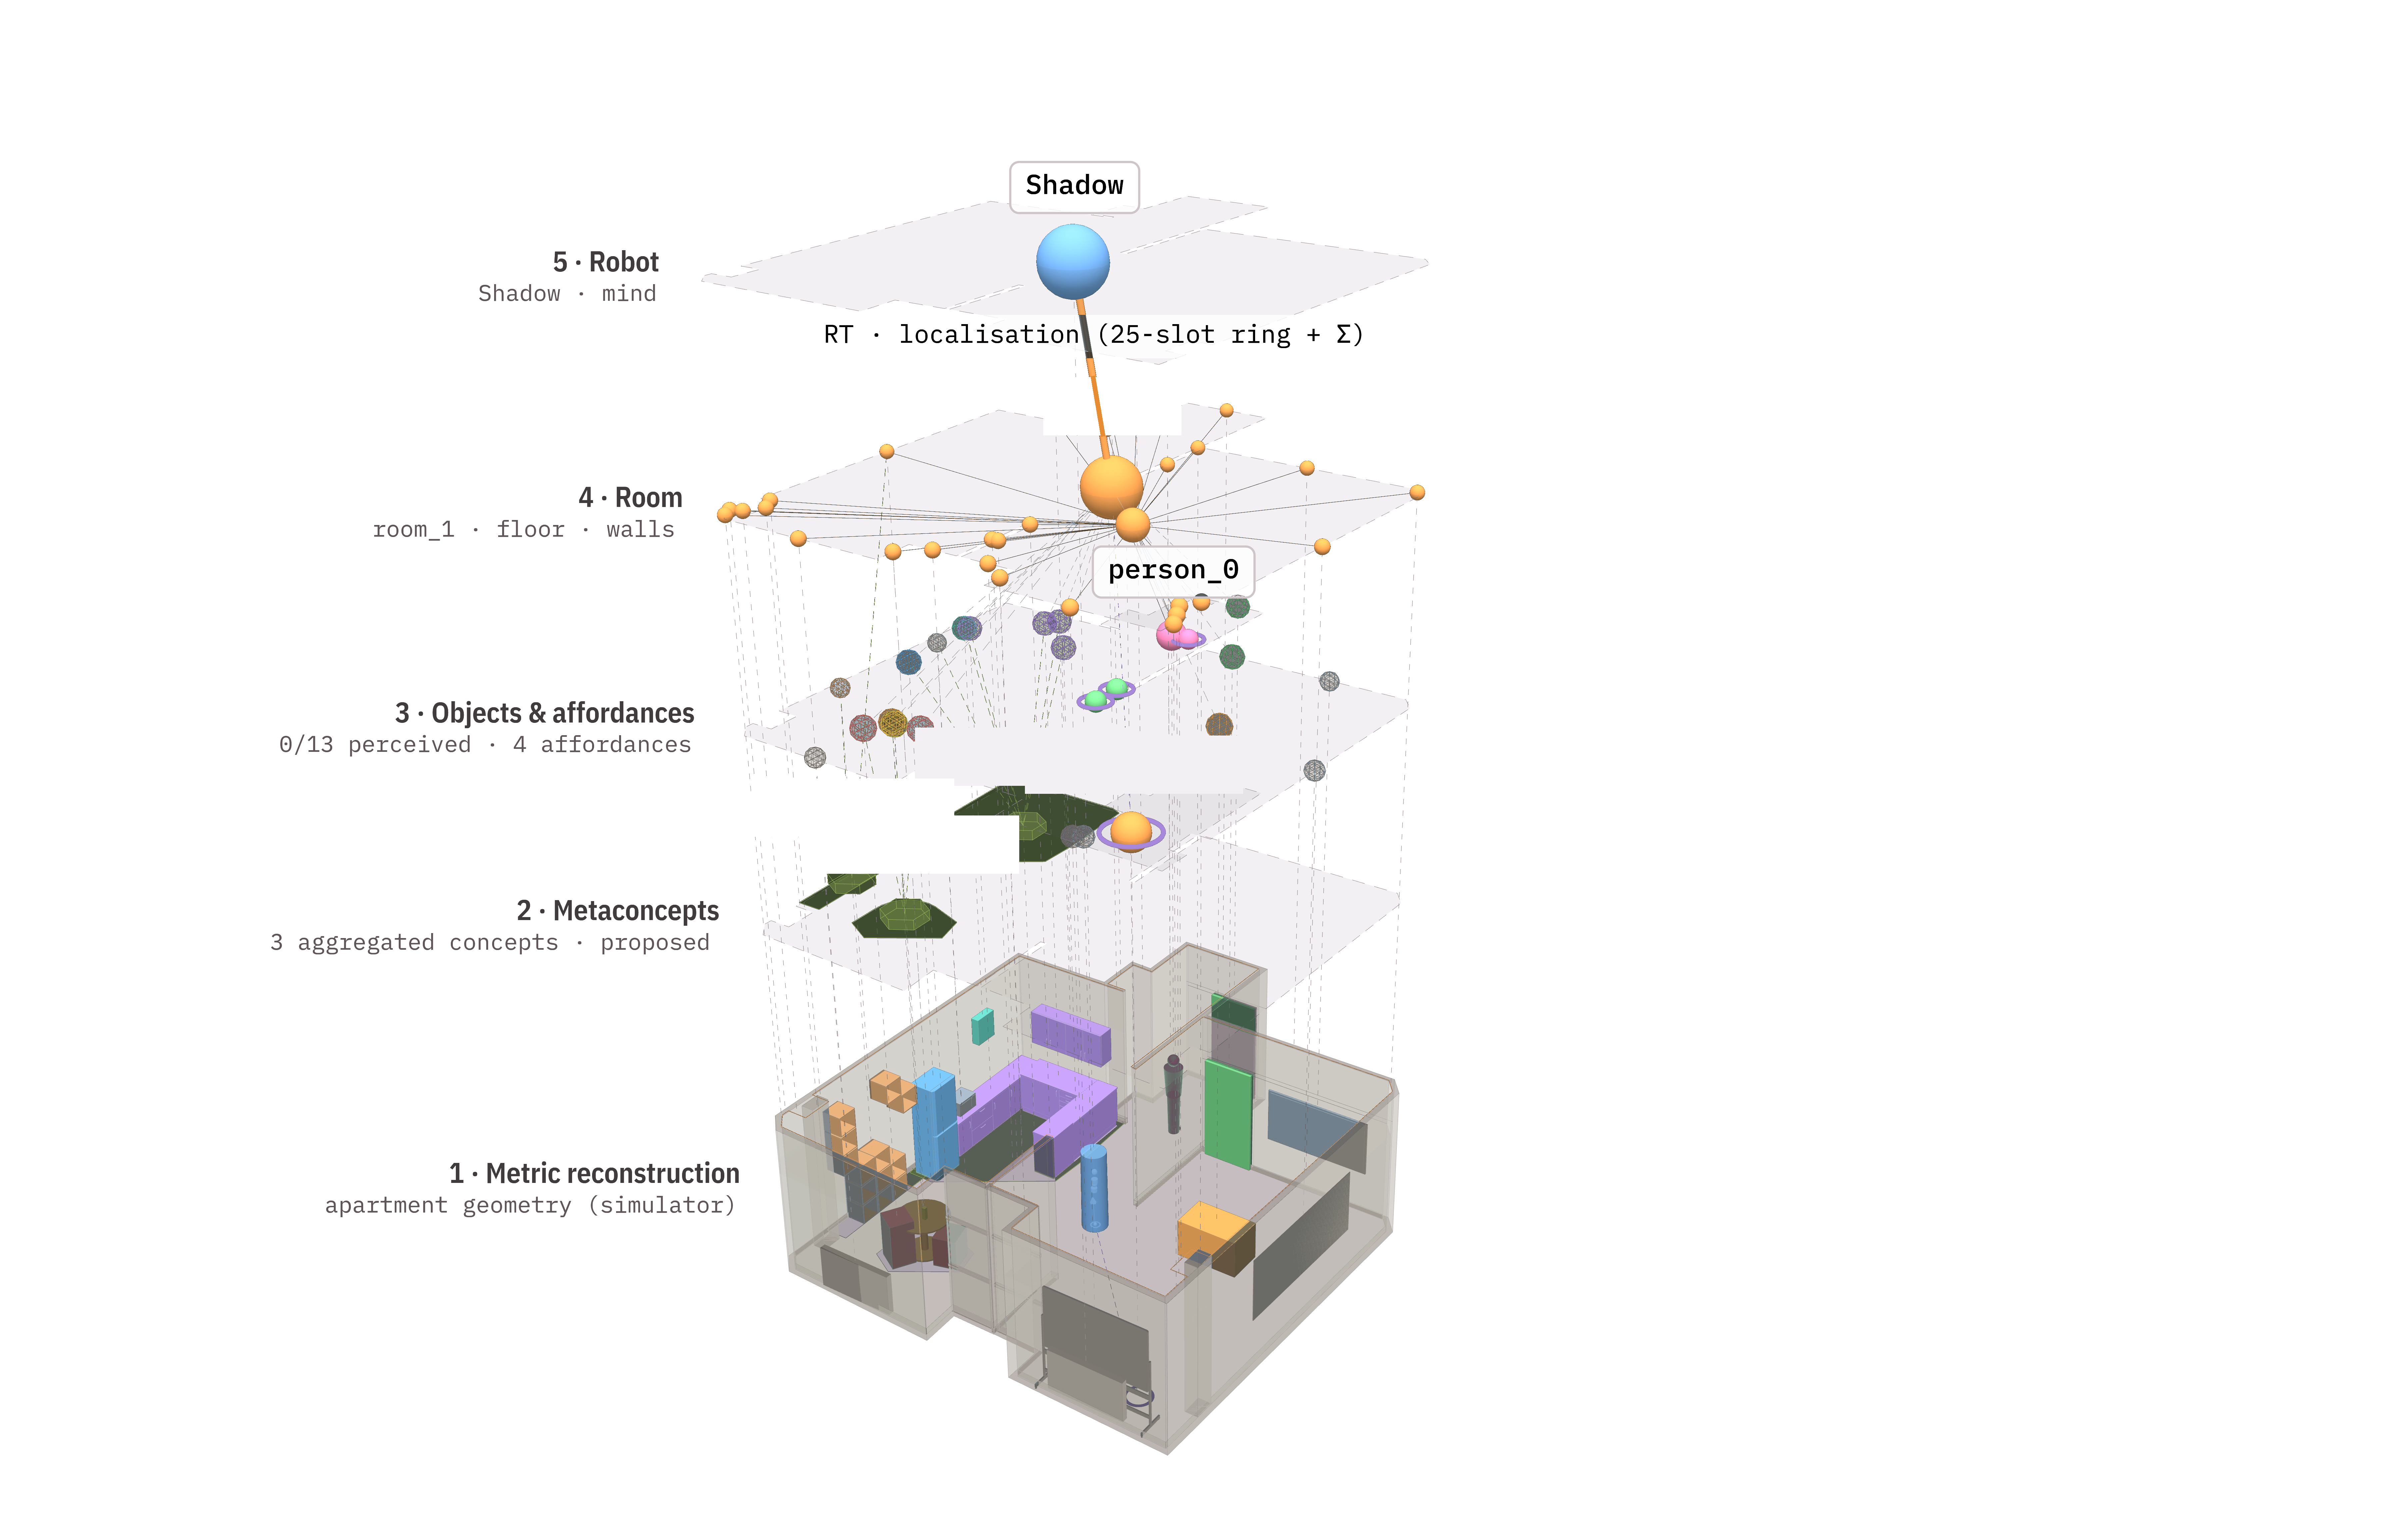
\includegraphics[width=\linewidth,trim=760 200 2850 420,clip]{figures/full_graph_white_clean.png}};
            \begin{scope}[x={(img.south east)}, y={(img.north west)}]
                % labels redrawn apart; the overlapping originals were removed from full_graph_white_clean.png
                \tikzset{lab/.style={draw=black!45, fill=white, rounded corners=1.5pt, inner sep=1.2pt,
                         font=\ttfamily\tiny}}
                \node[lab, anchor=east] at (0.690,0.800) {room\_1};
                \node[lab, anchor=west] at (0.425,0.505) {wall-shelf};
                \node[lab, anchor=west] at (0.470,0.462) {dinner-set};
                \node[lab, anchor=west] at (0.565,0.542) {kitchen-rig};
                \node[lab, anchor=west] at (0.775,0.515) {afford\_room};
                \fill[yellow!85!orange, draw=conceptc!80!black, thick] (0.80,0.585) circle (2.6pt);
                \node[draw=black!50, fill=white, rounded corners=1.5pt, inner sep=1.5pt,
                      font=\ttfamily\tiny, anchor=west] at (0.825,0.60) {chair\_34};
            \end{scope}
        \end{tikzpicture}
    \end{minipage}\hfill
    \begin{minipage}[c]{0.43\linewidth}
        \centering
        \resizebox{\linewidth}{!}{% belief-node.tex — schematic companion to Figure 2: one node of the graph as a belief.
% Uses the palette defined in vygotskian_machine_build.tex. Schematic, not data.
\begin{tikzpicture}[font=\scriptsize, >=Latex]
% ---------- the node card
\node[draw=conceptc, very thick, rounded corners=3pt, fill=conceptf, align=left, inner sep=4pt,
      text width=36mm, anchor=north west] (card) at (0,0) {%
  \tikz[baseline=-0.6ex]\fill[yellow!85!orange, draw=conceptc!80!black] (0,0) circle (2.4pt);\
  \textbf{\textcolor{conceptc!80!black}{chair\_34}}\\[1pt]
  owner: chair agent\\
  pose: mean $\mu$, covariance $\Sigma$\\
  existence: log-odds $\ell$\\
  parent: \texttt{room\_1}\\
  edge: transform $T$ and its $\Sigma$};
% ---------- floor sketch: pose belief seen from the robot
\begin{scope}[shift={(4.3,-2.15)}]
  \draw[black!55, thick] (0,0) -- (0,2.05) -- (3.0,2.05);
  \node[font=\tiny, text=black!55, anchor=south west] at (0,2.05) {room\_1 walls};
  % view cone
  \fill[wmc!25] (0.55,0.35) -- (2.75,1.65) -- (2.75,0.05) -- cycle;
  % robot
  \fill[bodyc!70] (0.55,0.35) circle (0.13);
  \draw[bodyc!80!black, thick, ->] (0.55,0.35) -- (0.9,0.55);
  \node[font=\tiny, text=bodyc!80!black, anchor=north] at (0.55,0.2) {robot};
  % chair belief: footprint at the mean, 2-sigma ellipse
  \draw[conceptc, thick, fill=conceptf, rotate around={25:(2.1,1.0)}] (2.1,1.0) ellipse (0.55 and 0.28);
  \draw[conceptc!80!black, fill=conceptc!45] (1.95,0.88) rectangle (2.25,1.12);
  \node[font=\tiny, text=conceptc!80!black, anchor=north] at (2.1,0.62) {$\mu$, $2\sigma$};
\end{scope}
% ---------- existence log-odds over time
\begin{scope}[shift={(0,-5.2)}]
  % segments
  \fill[wmc!18] (0.2,-0.75) rectangle (2.5,1.45);
  \fill[black!8] (2.5,-0.75) rectangle (4.6,1.45);
  \fill[bodyf] (4.6,-0.75) rectangle (7.0,1.45);
  \draw[->, black!60] (0,0) -- (7.35,0) node[anchor=west, font=\tiny, text=black!60] {time};
  \draw[->, black!60] (0,-0.75) -- (0,1.55) node[anchor=south, font=\tiny, text=black!60] {$\ell$};
  \draw[black!35, dashed] (0,0.0) -- (7.0,0.0);
  \draw[conceptc!85!black, very thick]
    (0.2,0.0) .. controls (0.9,0.7) and (1.6,1.05) .. (2.5,1.15)
    -- (4.6,1.15)
    .. controls (5.4,1.05) and (6.1,0.25) .. (6.9,-0.55);
  \node[font=\tiny, align=center, anchor=north] at (1.35,-0.78) {seen\\rises};
  \node[font=\tiny, align=center, anchor=north] at (3.55,-0.78) {occluded\\held};
  \node[font=\tiny, align=center, anchor=north] at (5.8,-0.78) {absent where\\detectable: falls};
\end{scope}
\end{tikzpicture}
}
    \end{minipage}
    \caption{Left: the output of \cortex{} in the simulated apartment, drawn by stratum: the robot (level~0),
    localised in \texttt{room\_1} (level~1); the objects and their affordances (level~2); and the aggregates fitted
    over them (level~3). The bottom stratum is the simulator's true geometry, shown for reference, and strata numbers
    give the drawing order, not the levels of Table~\ref{tab:lh_levels}. Right: a schematic of the node marked \texttt{chair\_34} on the left, as a belief
    owned by one agent, whose existence log-odds rises when the object is seen, is held while it is occluded, and
    falls only when it is absent where it could have been detected.}
    \label{fig:cortex_graph}
\end{figure}

\paragraph{Action and memory.}
A controller plans and follows paths. Its epistemic planner scores the actions that the concept agents offer, such as
looking at a door from a given place, by their expected free energy. An exploration drive turns this scoring into a
default behaviour. The robot explores the current room until further exploration yields too little information,
crosses the nearest uncrossed door, and returns in depth-first order. Three memory agents retain what the live graph
discards. The spatial memory stores each room the robot has left with the doors that connect it, and restores it as a
prior on return. The object memory keeps a persistent record of object instances. The episodic memory records the
robot's missions, their steps and how each ended. These memories provide the counts from which the priors and habits
of the Vygotskian machine will be learned.

\paragraph{The language agent.}
The language agent connects a person to all of these components through a vision-language model (VLM), Gemma 4
with 26 billion parameters, served by Ollama on an NVIDIA Jetson AGX Orin carried by the robot. Its design follows the principle
stated in the code as ``the model proposes, C++ decides''. The VLM sees a summary of the graph and the memories and can
act only by calling tools, and every call passes a deterministic gate that checks names against the graph and
arguments against the robot's capabilities. Extended behaviour is written in a small mission language (cross a door,
explore a room, approach an object, watch for a condition, if, repeat), and each mission is checked against the graph
and approved by the person before it runs. While a mission runs, robot events wake the model in restricted turns in
which it can look, query memory, stop and propose, but not act. Whether to ask the person or to make an assumption is
decided by a small rule over counts and costs. The agent also answers subjunctive questions with the robot's own
models, on an imagined copy of the room that can never write to the live graph. On that copy the controller answers
``would I fit?'', the perception models answer ``would I see it from there?'', and the episodic counts answer ``would
this route succeed?''. The imagination of Section~\ref{sec:lang_hierarchy:imagination} relies on these tools.

\paragraph{What is missing.}
\cortex{} can therefore perceive, hold beliefs, act, remember, talk and, when asked, imagine. Its VLM is used only when a
person speaks, nothing it knows becomes a prior, the robot never questions itself or imagines on its own initiative,
and the hundredth mission to the kitchen requires the same VLM calls as the first. The inner voice
(Section~\ref{sec:inner_speech}) and the cultural plane (Section~\ref{sec:lang_hierarchy}) address these gaps.

%     % =====================================================================================================
% vygotskian_internalisation.tex — The Vygotskian machine, part 2: internalisation (the inner voice)
%
% DRAFT (2026-11-19; first drafted 2026-11-18 as inner_speech_section.tex). A proposal section: it describes an
% architecture that is NOT yet implemented, grounded in the existing language_agent (robocomp/active_inference).
% Include from main.tex, in this order:
%     % =====================================================================================================
% vygotskian_machine.tex — The Vygotskian machine, part 1: the framing section
%
% DRAFT (2026-11-19). Opens the three-part proposal; a proposal, not a report of results.
% Include from main.tex, in this order:
%     \input{vygotskian_machine}
%     \input{vygotskian_cortex}
%     \input{vygotskian_internalisation}
%     \input{vygotskian_cultural_plane}
%     \input{vygotskian_experiments}
% with \addbibresource{vygotskian_machine.bib} and \usepackage{array} in the preamble.
% =====================================================================================================

\section{The Vygotskian Machine}
\label{sec:vygotskian}

According to Vygotsky, higher mental functions develop in accordance with one central law: each function first
emerges in interactions between people, and then within the individual \cite{vygotsky1978mind}. A child plans aloud
together with an adult before planning aloud alone, plans aloud alone before planning silently, and plans silently
before the plan is carried out without any words at all. Language is what carries the child through this sequence. It
is the means by which knowledge held by other people becomes the learner's own, and it is also the tool with which the
learner regulates its own actions while that knowledge is still new.

We propose to build a robot that follows this law, and we call it a \emph{Vygotskian machine}. The robot's higher
functions, such as its goals, its plans, the meaning it gives to a scene and what it expects to find in a room, are
first provided from outside. They come from the person who lives with the robot and from a vision-language model (VLM),
a neural network trained on images and text that carries a large share of human culture. The robot then internalises
these functions, first as an inner voice that asks questions, makes plans and imagines outcomes
(Section~\ref{sec:inner_speech}), and eventually as prior beliefs, accumulated counts of experience and habits that
need no language at all. The robot's automatic level consists of the Active Inference agents that build its hierarchy
of beliefs and control its movement. This automatic level is what the internalised knowledge ultimately shapes, and
it is also the level that language is called upon to assist whenever the situation exceeds its competence.

\begin{table}[ht]
    \centering
    \small
    \begin{tabular}{|>{\raggedright\arraybackslash}p{0.4\linewidth}|>{\raggedright\arraybackslash}p{0.5\linewidth}|}
        \hline
        \textbf{Vygotsky} & \textbf{The machine} \\ \hline
        Every higher function emerges first between people, and then within the individual
            & goals, plans and scene meaning arrive as a person's words and the VLM's culture, then become priors,
              plans and habits (Sections~\ref{sec:lang_hierarchy:culture}--\ref{sec:lang_hierarchy:sequencing}) \\ \hline
        Outer speech $\to$ private speech $\to$ inner speech $\to$ no speech
            & the VLM writes a mission; the inner voice rehearses and monitors it; the compiled habit runs without
              language (Eq.~\ref{eq:lh_habit}) \\ \hline
        Private speech rises with task difficulty and fades with mastery \cite{berk1992children}
            & the demand signal recruits the voice on surprise and leaves it idle when the automatic level copes
              (Section~\ref{sec:inner_speech:modes}) \\ \hline
        Scaffolding by a more knowledgeable other, withdrawn as competence grows \cite{wood1976role}
            & the VLM's prior weight is overtaken by the robot's own counts (Eq.~\ref{eq:lh_beta_prior}); the person
              is asked less as experience accumulates \\ \hline
        The zone of proximal development: what the learner can do only with help
            & situations outside the automatic level's competence but within reach with the VLM or the person;
              learning moves them inside \\ \hline
        Mediation by signs: language as a psychological tool
            & the VLM's output is never accepted as belief; instead, it structures what the robot's own models do by
              proposing, sequencing and choosing what to imagine (Table~\ref{tab:lh_roles}) \\ \hline
    \end{tabular}
    \caption{Vygotsky's account and its counterpart in the proposed machine.}
    \label{tab:vygotskian_mapping}
\end{table}

\paragraph{Internalisation in Active Inference.}
Within the framework of this document, the passage from outer to inner speech can be given a precise
interpretation. Culture enters the generative model, the robot's probabilistic model of how its observations are
produced, in two places. It enters as prior beliefs and preferences, which describe what a room is for, which objects
tend to appear together and which outcomes are acceptable, and it enters as candidate policies, that is, sequences of
actions, which are scored by their expected free energy. Experience then internalises this culture in the two
corresponding places. The priors are progressively replaced by counts of what the robot itself has observed, and the
candidate policies that continue to succeed become part of the habit prior, a learned preference over policies. The
machine's dependence on language for routine matters should therefore decrease with experience, while remaining for
situations that are novel, social or structural.

\paragraph{Organisation.}
Section~\ref{sec:cortex} describes CORTEX, the architecture on which the machine is built. CORTEX already includes a
language agent, and the machine is defined by what it adds to that architecture. Section~\ref{sec:inner_speech}
develops internalisation. It treats the inner voice as an epistemic action, that is, an action taken to gain
information, and describes the attention modes that call on the voice and release it, as well as the learning that the
voice drives. Section~\ref{sec:lang_hierarchy} develops the cultural plane. It explains how the VLM is connected to the
belief hierarchy in three roles, namely culture, sequencing and imagination, under the rule that the language model
proposes and the generative models dispose.

\paragraph{The internalist contrast.}
According to the opposing, internalist view, language evolved first as an internal system for thought and was only
later used to communicate \cite{berwick2016why}. We use this view as a contrast rather than as a rival, because the
distinction it draws between the faculty of language and the content that language carries
(Section~\ref{sec:inner_speech:why_lm}) is what makes the Vygotskian claim testable. A machine that has a
compositional inner language but no culture serves as the \emph{non-Vygotskian control}. Its inner language is built
by library learning, the gradual collection of reusable sub-programmes, from the robot's own experience alone
(Section~\ref{sec:inner_speech:library}). If this control machine performs as well as the machine fed with culture in
situations far from anything the robot has seen, then culture is not doing the work that the name of the machine
claims for it.

\paragraph{Prior uses of the idea.}
Mirolli and Parisi argued for a Vygotskian cognitive robotics in which language serves as a cognitive tool as well as
a means of communication \cite{mirolli2011towards}, and Colas et al.\ proposed Vygotskian autotelic agents that
internalise language and culture to imagine and pursue their own goals \cite{colas2022language}. The present proposal
shares their premise but differs from them in three respects. First, internalisation is formalised within Active
Inference, as culture that enters priors and policies and gradually settles into counts and habits. Second, the
internalised knowledge acts on a probabilistic belief hierarchy whose evidence rules and cavity messages, which exclude
a belief's own contribution from the evidence it receives, prevent the hierarchy from confirming itself. Third, an
attention mechanism decides, from moment to moment, whether language is needed at all.

\paragraph{Two bitter lessons.}
Any proposal that builds knowledge into a robot has to respond to what Sutton called the bitter lesson. According to
Sutton, across seventy years of AI research, general methods that scale with computation, search and learning have
eventually outperformed methods that build in what their designers know \cite{sutton2019bitter}. Chess programs built
on human expertise were overtaken by search, and speech and vision systems built on expert-designed features were
overtaken by statistical learning. A robot whose levels 1 to 3 are generative models written by its designers, and
whose prior about kitchens is a table of log-odds written by hand, is open to the same criticism. A second lesson has
recently been drawn from the success of the first. Verbelen argues that ``the main idea behind modern AI is not
learning. It is amortisation'' \cite{verbelen2026newbitter}. In this view, training converts expensive inference into
reusable structure, so that a foundation model is a store of distilled past computation. Amortisation works when the
future resembles the past and fails when it does not. From this follows the new bitter lesson, that ``intelligence
cannot be fully amortised''. A system that must face a changing world needs, in addition to what it has precomputed,
three capabilities that amortisation does not supply, namely learning online during deployment, exploring actively to
reduce its own uncertainty, and forming new hypotheses when the old model no longer fits.

\paragraph{Where the Vygotskian machine stands.}
The two lessons pull in opposite directions. The first advises against handcrafting knowledge and in favour of using
what large-scale training has learned. The second warns that what large-scale training has learned is not enough, and
that a system must continue to perform inference. Neither lesson says how a system should combine the two, and such a
combination is what the Vygotskian machine proposes. Its novelty lies in four aspects.

\begin{enumerate}[(i)]
    \item \emph{Amortised culture as a proposal, never as a belief.} The VLM is the most amortised object
    available, since it contains human culture distilled by training at scale. The machine treats it as exactly
    that, the product of a general method, and uses it where Sutton's lesson says such methods should be used,
    namely to replace the hand-written parts of the system. The authored log-odds of the kitchen prior become priors
    elicited from the VLM, and the meaning of a room, which no designer has written down, also comes from the VLM.
    The machine never uses the VLM's output as its belief. Instead, the VLM's proposals are scored by ongoing
    inference against evidence, including evidence that something is absent, and they enter the generative model as
    pseudo-counts, imaginary prior observations that the robot's own experience gradually outweighs
    (Eq.~\eqref{eq:lh_beta_prior}).
    \item \emph{Internalisation is amortisation by the robot, with a way back.} The robot amortises its own
    ongoing inference, in the sense that what the inner voice works out in focused mode settles into priors, counts
    and habits that no longer need language. This process is the internalisation described by Vygotsky's law, and it
    is also the amortisation of the second lesson, carried out by the agent itself, on its own data, while it acts.
    Each compiled habit carries with it the assumptions under which it was learned
    (Section~\ref{sec:lang_hierarchy:sequencing}). When the probability of those assumptions falls, the habit is set
    aside and ongoing inference takes over again.
    \item \emph{A signal that decides when amortisation is enough.} The new bitter lesson states that
    amortisation fails when the situation is novel, but it does not say how an agent notices that this has happened.
    In the machine, this decision is made continuously by a demand signal, which is a prediction error weighted by
    its precision, that is, by the confidence placed in it (Section~\ref{sec:inner_speech:modes}). While the amortised
    levels predict well, the inner voice either remains silent or imagines, and a surprise calls on ongoing inference
    mediated by language. Private speech in children behaves in the same way, increasing with task difficulty and
    fading as the child gains mastery.
    \item \emph{The three missing properties, each with its own mechanism.} Online learning consists of the
    gradual replacement of the VLM's pseudo-counts by experience and the growth of the habit prior with experience.
    Active exploration takes the form of the inner question, treated as an epistemic action and scored by its
    expected information gain (Section~\ref{sec:inner_speech:questions}). New hypotheses arise from surprise at the
    level of the model itself. When the evidence for an arrangement of objects collapses, or when a class of objects
    repeatedly fails to fit where it is expected, the VLM proposes a new structure and the robot's own models test
    it. In every case, the VLM generates candidates and the robot's models evaluate them.
\end{enumerate}

The machine thus interprets the first lesson as a reason to take culture from a learned model instead of writing it
by hand, and the second as a reason to keep that culture outside the belief state, where ongoing inference can correct
it. Vygotsky's account supplies the developmental sequence that connects the two lessons, in which knowledge is first
borrowed from others, then used through speech, and finally internalised until it no longer needs speech.

\paragraph{What would demonstrate that the paper's goal has been achieved?}
The central claim rests on three predictions. First, the non-Vygotskian control falls behind the machine fed with
culture in proportion to the novelty of a situation (P7 in Section~\ref{sec:inner_speech:predictions}). Second, the
machine's use of language behaves as private speech does, increasing with difficulty and decreasing with mastery
(P8). Third, the scaffold provided by the VLM is withdrawn, so that as confirmed rooms and successful missions
accumulate, the number of calls to the VLM falls while task success is maintained (L6 in
Section~\ref{sec:lang_hierarchy:predictions}).

%     % =====================================================================================================
% vygotskian_internalisation.tex — The Vygotskian machine, part 2: internalisation (the inner voice)
%
% DRAFT (2026-11-19; first drafted 2026-11-18 as inner_speech_section.tex). A proposal section: it describes an
% architecture that is NOT yet implemented, grounded in the existing language_agent (robocomp/active_inference).
% Include from main.tex, in this order:
%     \input{vygotskian_machine}
%     \input{vygotskian_internalisation}
%     \input{vygotskian_cultural_plane}
% and add the shared bibliography:  \addbibresource{vygotskian_machine.bib}
% Packages used: amsmath, amssymb, enumitem (already loaded by main.tex) and array, which main.tex does not
% load yet: add \usepackage{array} to its preamble.
% Labels keep their original sec:inner_speech:* prefix so that existing cross-references do not break.
% =====================================================================================================

\section{Internalisation: the Inner Voice}
\label{sec:inner_speech}

The robot described so far uses language in one direction only: a person speaks, and a language agent turns
the request into commands for the controller, grounded in a textual digest of the belief graph. This section
proposes to turn that capability inward, which constitutes the internalisation step of the Vygotskian machine
(Section~\ref{sec:vygotskian}). We argue that a language model embedded in an Active Inference
architecture can play the role that inner speech plays in human cognition, namely that of a serial and
compositional medium in which the agent poses questions to itself, generates hypotheses, rehearses plans and
replays its past. We further argue that this role follows naturally from the epistemic component of expected free
energy. The proposal is presented together with the constraints that prevent such a voice from becoming a source
of confabulated beliefs, and with the experiments that would falsify it.

\subsection{Motivation: from talk to thought}
\label{sec:inner_speech:motivation}

Two theoretical traditions disagree about the origin of inner speech, but they agree about its function. According
to the developmental view that gives the machine its name, inner speech is social speech that the child gradually internalises, abbreviates and
turns into a tool for self-regulation \cite{vygotsky1986thought}. According to the internalist view, which we use
as the point of contrast throughout this section, human language evolved first as an internal system for structuring thought, and its use for
communication is a later externalisation \cite{berwick2016why}. Contemporary reviews treat inner speech as
functionally involved in planning, problem solving, self-monitoring and the maintenance of goals in working memory
\cite{aldersonday2015inner}, and language more generally as a cognitive technology that lets a learner manipulate
discrete, recombinable tokens rather than raw percepts \cite{clark1998magic}.

Large language models provide a striking example of the developmental route. They are trained exclusively on
communicative text, yet their performance improves measurably when they produce intermediate reasoning in that
same medium before answering, a technique known as chain-of-thought \cite{wei2022chain}. In this sense, a system
built for communication becomes better at reasoning when it addresses its speech to itself. Our language agent is
at a comparable point in its own development. It was built to converse with a person, and the question we ask is
what it contributes once its speech is addressed to the robot itself.
Section~\ref{sec:inner_speech:why_lm} returns to the internalist contrast, and Section~\ref{sec:inner_speech:library}
turns it into a control experiment.

\subsection{Inner questions as epistemic actions}
\label{sec:inner_speech:questions}

In Active Inference, policies are scored by expected free energy, whose epistemic term rewards the expected
reduction of uncertainty about hidden states \cite{friston2017process, parr2022active}. A question can be
regarded as the linguistic expression of exactly this quantity, since it names a hidden variable whose value is
uncertain and whose resolution is expected to matter. We therefore model an inner question as a persistent object
\begin{equation}
    \mathcal{Q} = \big\langle\, e,\; \mathcal{H},\; q(h),\; \mathcal{P},\; b,\; s \,\big\rangle ,
    \label{eq:inner_question}
\end{equation}
where $e$ is the triggering event (for example an obstacle no concept agent explains), $\mathcal{H}$ a finite set
of named hypotheses (``a chair'', ``a box'', ``unknown''), $q(h)$ the current posterior over them, $\mathcal{P}$
the set of pending predictions, $b$ a budget in time and motion, and $s \in \{\text{open},\text{resolved},
\text{abandoned}\}$ its status. Questions are organised as a stack, in the sense of a \emph{question under
discussion} \cite{roberts2012information}, so that ``is it a chair?'' is a sub-question whose answer partially
resolves the parent question ``what is this?''. It is the question object, and not the language model's context
window, that carries the state of the reasoning from one step to the next.

\paragraph{One step of the loop.}
Given $\mathcal{Q}$, the language model proposes a test, which consists of an epistemic action $a$ (turning
towards the anomaly, approaching it, looking with the front camera) together with the outcome that each hypothesis
predicts. The value of the test
is its expected information gain minus its cost,
\begin{equation}
    V(a) \;=\; \underbrace{H\!\left[q(h)\right] \;-\; \mathbb{E}_{p(o \mid a)}\!\left[ H\!\left[q(h \mid o, a)\right]
    \right]}_{I(h;\,o \mid a)} \;-\; c(a),
    \label{eq:inner_value}
\end{equation}
which is the negative of the epistemic part of expected free energy with an explicit action cost. The test is
executed only if $V(a) > 0$ and the action passes the same deterministic gate that already validates every
command the language agent issues. When the observation $o$ arrives, the posterior is updated by the concept
agents' own likelihoods,
\begin{equation}
    q(h \mid o, a) \;\propto\; p(o \mid h, a)\, q(h),
    \label{eq:inner_update}
\end{equation}
and the loop continues, spawns a sub-question, or terminates when
\begin{equation}
    H\!\left[q(h)\right] < \eta \quad\lor\quad \max_a V(a) \le 0 \quad\lor\quad b \text{ exhausted}.
    \label{eq:inner_stop}
\end{equation}
This stopping rule is what distinguishes reasoning from rumination. A loop with no expected information left to
gain is closed, possibly with the answer ``unknown'', and the event that triggered it is habituated, that is,
ignored for a refractory period.

\paragraph{The grounding constraint.}
The central design rule is that the language model may suggest hypotheses but only perception may decide between
them; in short, \emph{the language model proposes and perception disposes}. Text produced by the model may
introduce hypotheses, predictions and tests, but it may never change a posterior. Only the likelihood
$p(o \mid h, a)$ in \eqref{eq:inner_update}, computed by the perceptual agents from sensor data, can do so. This
rule is the counterpart, on the side of beliefs, of the rule that the language agent already enforces for actions,
under which every proposed command is validated in C++ against the belief graph before it reaches the controller.
Without it, a language loop addressed to itself would be a closed system in which text is conditioned only on
text, and it would converge on its own confabulations.

\paragraph{The proposer as a calibrated prior.}
The hypotheses the model names, and the probabilities it attaches to them, encode world knowledge the robot has
not acquired by itself (``chairs come with tables''). We treat this knowledge as a prior whose weight must be
earned through demonstrated accuracy. Let
$\pi_{\text{LM}}(h \mid x)$ be the proposer's distribution in context $x$ and $n_x(h)$ the robot's own counts of
resolved questions in that context. The prior entering \eqref{eq:inner_update} is
\begin{equation}
    q_0(h \mid x) \;\propto\; \pi_{\text{LM}}(h \mid x)^{\beta_x}\, \big(\alpha + n_x(h)\big),
    \label{eq:inner_prior}
\end{equation}
a tempered product of the proposer and a Dirichlet over experience, where $\beta_x \in [0,1]$ is set from the
proposer's measured calibration in that context (for instance from its Brier score on past questions). Early in
the robot's life the proposer dominates this prior, and as the counts accumulate, the robot's own experience
progressively replaces the knowledge borrowed from the language model. The same conjugate form already governs the language agent's decision to ask a person or to assume
that they moved an object, where a Beta posterior over the person's past answers is compared against the costs of
asking and of being wrong.

\subsection{Attention, automaticity and the wandering mind}
\label{sec:inner_speech:modes}

A human driver on an easy road can steer without attending to the road, which leaves the mind free to plan, imagine
or recall, and attention returns to the task as soon as something unexpected happens
\cite{smallwood2015science, christoff2016mind}. In Active Inference this phenomenon is described in terms of
precision. While prediction errors are small and the habitual policy is reliable, attention, understood as the
precision assigned to sensory prediction errors, can be withdrawn from the task, and a surprise raises it again
\cite{feldman2010attention}. The account in which habitual and deliberative control are arbitrated according to
their relative uncertainty \cite{daw2005uncertainty} has the same structure.

The architecture already separates the two systems. The controller and the concept agents form an automatic layer
that drives, avoids obstacles and executes missions without the language model, while the language agent provides
the deliberative voice. We propose to make the allocation of this voice explicit through a scalar \emph{demand}
signal, computed without the language model each time the textual digest of the belief graph is updated,
\begin{equation}
    D_t \;=\; \sum_{k} \pi_k\, \varepsilon_{k,t}^{2} \;+\; \lambda\, \mathbb{1}\!\left[\text{person active}_t\right],
    \label{eq:inner_demand}
\end{equation}
where $\varepsilon_{k,t}$ are normalised prediction errors reported by the agents (unexplained residual occupancy,
flips of existence or door beliefs, localisation uncertainty, stalled or failed mission steps, controller refusals)
and $\pi_k$ their precisions. Three operating modes then follow from two thresholds with asymmetric hysteresis:
\begin{equation}
    m_t =
    \begin{cases}
        \textsc{focused}    & D_t > \theta_{\text{hi}},\\[2pt]
        \textsc{wandering}  & D_\tau < \theta_{\text{lo}} \;\; \forall\, \tau \in [t - T, t],\\[2pt]
        \textsc{monitoring} & \text{otherwise.}
    \end{cases}
    \label{eq:inner_modes}
\end{equation}
Entering \textsc{wandering} requires demand to stay low for a dwell time $T$; leaving it requires a single sample
above $\theta_{\text{hi}}$. The robot is therefore slow to let its attention drift away from the task and
immediate in returning to it. Safety never depends on this arbitration, because the controller's reflexes act on
their own and the deliberative voice engages only after the reflex has acted, just as a driver becomes aware of a
hazard only after having braked.

\paragraph{Focused mode} runs the question loop of Section~\ref{sec:inner_speech:questions} on the triggering
event. \paragraph{Monitoring mode} makes no calls to the language model, so that the voice is ready to engage but
remains silent.

\paragraph{Wandering mode.}
When the voice is freed from the task, it is seeded with one recent experience chosen by salience, such as an
episode that ended unresolved, a failure, an object that changed, or an upcoming goal. The output of each step,
together with an associative retrieval from episodic memory, seeds the next step, so that the chain of thoughts
drifts in the way spontaneous thought does \cite{christoff2016mind}. The voice has access only to memory queries and to the architecture's imagination tools,
which simulate observations and outcomes on a copy of the belief graph; it can neither act nor write beliefs. Its
products are of three kinds: counterfactuals over past episodes (``had the door been open, the crossing would have
taken 40\,s less''), hypotheses to be tested later, and prospective plans (``if the door is shut on the way back,
the route through the next room is shorter''). Functionally, this corresponds to the role of the brain's default
network in simulating the past and the future \cite{buckner2008brain}, and to the offline replay and model reduction that Active Inference assigns
to rest and sleep \cite{friston2017curiosity, hobson2012waking}. Replay is prioritised by the expected gain of the
memory it revisits \cite{mattar2018prioritized}.

\paragraph{Source monitoring.}
Humans occasionally misremember imagined events as perceived ones \cite{johnson1993source}, and the robot must not
make this error.
Everything produced while wandering is stored with an \emph{imagined} provenance, separate from the factual
episodic record, and enters the learning loop only as a hypothesis to be tested, never as evidence.

\subsection{What the return to reality gives the automatic layer}
\label{sec:inner_speech:return}

The transition from \textsc{wandering} to \textsc{focused} cancels the chain of thought in progress (its state is
kept, so that it may resume if demand subsides) and devotes the voice entirely to the surprising event. This return
to reality serves the automatic layer on three timescales.
\begin{enumerate}
    \item \textbf{Decision.} A surprise indicates that the automatic layer has left its domain of competence, and
    outside that domain its only responses are to retry, to stop or to fail. The voice adds the re-interpretation of
    the scene, arbitration between goals, re-planning through the remembered topology, and recourse to a person.
    \item \textbf{Attention.} The voice can raise precision where it matters, by orienting sensors, increasing a
    detector's rate in a region, or passing a hypothesis to the concept agents as a spatial prior. Such a prior has
    bounded weight, so that it may accelerate the recognition of an object that is present but cannot create one
    that is absent, which preserves the grounding constraint.
    \item \textbf{Teaching.} Each resolved surprise is a labelled example that the automatic layer could not have
    produced alone. For instance, an unexplained residual later identified as a chair is a false negative of the
    chair detector, a door that is repeatedly shut in the evening becomes a prior, and a recovery that repeatedly
    succeeds becomes a branch of the controller's behaviour tree. In this way the domain of competence grows and the
    situations that require the voice become rarer, which is the classical progression from effortful to autonomous
    skill \cite{fitts1967human}.
\end{enumerate}
Plans prepared while wandering act as a store of precomputed solutions, so that when the anticipated situation
occurs, the focused voice verifies an existing plan instead of composing a new one. The return ends with an
explicit release, in which spatial priors are cleared, safety margins are restored and the automatic layer is
confirmed to be back within its competence. Without this release, every surprise would leave the robot permanently
vigilant.

\subsection{Relation to chain-of-thought reasoning}
\label{sec:inner_speech:cot}

Chain-of-thought reasoning is a form of inner speech in the functional sense, although of a specific kind, and
comparing the two clarifies the design (Table~\ref{tab:inner_cot}). Plain chain-of-thought is convergent and
ungrounded, in that each token is conditioned only on previous tokens until an answer is produced, after which the
trace is discarded. Reasoning becomes grounded when it is interleaved with action and observation
\cite{yao2023react}. Our focused loop is of this kind, with the additional property that the observation, through
\eqref{eq:inner_update}, rather than the next token, determines the direction the reasoning takes. The wandering
voice is closer to plain chain-of-thought in its isolation from perception, but it is divergent rather than
convergent, it can be interrupted, and its products persist.

\begin{table}[ht]
    \centering
    \small
    \begin{tabular}{|>{\raggedright\arraybackslash}p{0.19\linewidth}|>{\raggedright\arraybackslash}p{0.22\linewidth}|>{\raggedright\arraybackslash}p{0.24\linewidth}|>{\raggedright\arraybackslash}p{0.24\linewidth}|}
        \hline
                                & \textbf{Chain-of-thought} & \textbf{Focused voice} & \textbf{Wandering voice} \\ \hline
        Goal                    & answer a given question   & resolve a given surprise & none given; seeded by salience \\ \hline
        Dynamics                & convergent                & convergent             & divergent, associative \\ \hline
        Contact with the world  & none                      & thought--action--observation & none (imagination only) \\ \hline
        Persistence             & discarded                 & question objects, beliefs, lessons & imagined store, hypotheses \\ \hline
        Interruptible           & no                        & yes                    & yes, resumable \\ \hline
        Latency budget          & n/a                       & $\sim$1\,s, no extended thinking & unbounded, extended thinking \\ \hline
    \end{tabular}
    \caption{Chain-of-thought compared with the two modes of the proposed inner voice.}
    \label{tab:inner_cot}
\end{table}

Two practical consequences follow. First, extended reasoning should take place \emph{when there is time, not when
there is pressure}. In the deployed language agent the model's extended thinking is disabled, because a model
operating in thinking mode spent 3\,000--6\,000 tokens (40--80\,s) before each tool call. Such a delay is
incompatible with the focused mode but costs nothing in the wandering mode, where extended thinking can be enabled
with a large budget and pre-empted at any moment. In this way slow reasoning is carried out in advance, and fast
reasoning makes use of its results. Second, chain-of-thought traces are known not always to reflect the
computation that produced the answer \cite{turpin2023language}, as human verbal reports do not always reflect the
causes of behaviour \cite{nisbett1977telling}. The faithful record of the robot's reasoning is therefore the
structured record of hypotheses, predictions, observations and posterior updates, not the generated text. Finally,
wandering chains whose hypotheses were later confirmed by perception form a corpus of reasoning verified against the world,
which could be used to fine-tune the local model in the manner of self-taught reasoning \cite{zelikman2022star},
with perception, rather than a known answer, as the filter.

\subsection{Consequences for belief and learning}
\label{sec:inner_speech:learning}

The question loop changes the way beliefs evolve in two respects. Within an episode, uncertainty is reduced where surprise
occurred rather than where the sensors happened to point, which is efficient but leaves the rest of the map less
examined and makes the robot's own data a biased sample; a decaying novelty term \cite{schwartenbeck2019curiosity}
and importance weighting of learned statistics are required to correct this. Across episodes, every closed
question is a labelled example, and learning proceeds at four timescales (Table~\ref{tab:inner_learning}).

\begin{table}[ht]
    \centering
    \small
    \begin{tabular}{|>{\raggedright\arraybackslash}p{0.14\linewidth}|>{\raggedright\arraybackslash}p{0.37\linewidth}|>{\raggedright\arraybackslash}p{0.37\linewidth}|}
        \hline
        \textbf{Timescale} & \textbf{What changes} & \textbf{Where, in this architecture} \\ \hline
        Seconds   & posterior over the hypotheses of one question         & the question object \eqref{eq:inner_question} \\ \hline
        Days      & priors: where objects are, which doors are shut, what moves & long-term object and topological memory, as Dirichlet counts \\ \hline
        Weeks     & likelihoods: detector and concept models              & false negatives and positives labelled by resolved questions \\ \hline
        Slow      & structure: new categories                             & recurrent, mutually similar ``unknown'' resolutions named by the voice and proposed as a new concept \\ \hline
    \end{tabular}
    \caption{Learning driven by the inner-question loop.}
    \label{tab:inner_learning}
\end{table}

The last row of the table engages most directly the hypothesis that language serves as a medium for thought,
since a cluster of anomalies that no existing concept can explain becomes learnable once it has been named. The
loop also learns about its own operation. The salience weights $\pi_k$ in \eqref{eq:inner_demand} are adjusted
according to the information that each trigger actually yielded, the option of asking a person is weighed against
that of looking, and loops that repeatedly resolve the same way are compiled into
reflexive rules, so that the number of language-model calls per hour should \emph{decrease} as competence grows.

\subsection{Why a language model: generation versus evaluation}
\label{sec:inner_speech:why_lm}

Since none of the above requires a person, it is natural to ask what a language model contributes to an
architecture that already performs inference and action selection. Our answer rests on a division of labour. Expected
free energy evaluates policies and Bayesian updating weighs hypotheses, but both operate over a space that has
already been enumerated: each concept agent carries a fixed generative model, policies must be listed before they
can be scored, and Bayesian model reduction can prune structure but not invent it \cite{friston2017curiosity}.
Whatever falls outside the given models remains an unexplained residual. A language model is weak where this
machinery is strong, since its confidences are not calibrated posteriors and it has no access to the sensors, and
it is strong where this machinery is weak, since it is an inexpensive and broad generator of hypotheses,
explanations and plans. We therefore use it only as a \emph{proposal distribution}, that is, as a source of
candidates in a generate-and-test loop whose test is carried out by active inference:
\begin{itemize}
    \item \emph{Hypotheses outside the built-in models.} A residual blob can be proposed to be a bag, a toppled
    chair or a robot vacuum, none of which any concept agent represents; the question loop then tests them.
    \item \emph{Amortised policy search.} Instead of enumerating multi-step policies, the model writes a few
    candidate missions, which are small programs in the mission language; the gate validates them and expected
    free energy scores them.
    \item \emph{Relational binding across agents.} The agents' representations (signed distance fields, occupancy
    grids, existence log-odds, episodic records) are mutually incompatible, whereas a sentence such as ``the chair
    that was not next to the table in the room behind door~3 yesterday'' binds them in a single query that no
    individual agent could formulate.
    \item \emph{Explanation from few examples.} After a single surprise the model can propose which variable
    mattered (``the door is shut because it is evening''), turning one episode into a testable generalisation.
    \item \emph{Abstraction and naming.} Episodes are compressed into reusable lessons, and recurrent unknowns are
    named, which is what makes them candidates for a new concept (Table~\ref{tab:inner_learning}).
\end{itemize}
The use of language, rather than an arbitrary learned embedding, matters for three reasons. Language is discrete
and compositional, so that new hypotheses and plans can be assembled from known parts; it is inspectable, so that
deterministic gates can parse and check it and people can audit it; and, once the robot thinks in it,
communication with a person comes at no further cost.

\paragraph{Where the knowledge comes from.}
This argument raises a difficulty for the internalist thesis introduced in the motivation. If the inner voice
precedes the outer one, the common-sense knowledge on which the value of the proposer rests cannot have arrived
through communication, and yet a language model acquires all of that knowledge from human text, that is, from the
outer voices of other people. The difficulty disappears once the language \emph{faculty} is distinguished from its
\emph{content}. The internalist claim concerns the former, namely a computational system for building unbounded
hierarchical structures, which is available for thought before it is used for communication
\cite{hauser2002faculty, berwick2016why}. It makes no claim that what a person knows was acquired without
language. Human knowledge has three sources: core systems for objects, agents, number and space, present before
learning \cite{spelke2007core}; individual experience; and, once outer language exists, cumulative cultural
transmission, which supplies most of what an adult knows \cite{tomasello1999cultural}. Even on the internalist
view, the inner voice of a modern human is filled largely by the outer voices of others.

The architecture has the same three sources of knowledge, arranged differently. The hand-built generative models
of the concept agents play the role of \emph{core knowledge}, since they are given before experience and limited
to a few domains. The robot's own counts $n_x(h)$ in \eqref{eq:inner_prior} constitute \emph{individual
experience}. The language model plays the role of \emph{culture}, that is, of knowledge distilled from a
community's communication and inherited by this individual at birth. The robot therefore resembles a child born
into a culture more than an early hominin, and its inner voice is Vygotskian in origin, because both its format and
its content were learned from outer speech. Two consequences follow. First, the proposal does not demonstrate the
internalist thesis and should not be read as doing so. Its claim is functional, namely that an inner use of
language has epistemic value independently of communication, and this claim holds whatever the origin of the
language system. Second, the format and the content of the voice can in principle be separated, which turns the
question into an experiment. A compositional generator over the robot's own concepts and mission language, trained
only on the robot's experience, would supply the format without the culture. Section~\ref{sec:inner_speech:library}
describes such a generator.

\subsection{A control experiment: a language-like format without human culture}
\label{sec:inner_speech:library}

We claim that a Vygotskian machine needs culture and not merely a language-like format, and this claim can be
tested only against a machine that has the format without the culture. Library learning, a technique from the
field of program induction, offers a concrete candidate for such a machine. DreamCoder \cite{ellis2021dreamcoder} learns to
solve tasks by writing programs and, at the same time, learns the language in which it writes them. It maintains a
library $\mathcal{L}$, initially a small base language of typed primitives, and a prior $P(\rho \mid \mathcal{L})$
over programs $\rho$ given by a probabilistic grammar over that library, under which a program that reuses library
functions is short and therefore probable. Each task $x$ supplies a likelihood $P(x \mid \rho)$, in the original
work usually the indicator that $\rho$ solves $x$. The system seeks the library and the sets of solutions
$\mathcal{F}_x$ that jointly maximise
\begin{equation}
    P(\mathcal{L}) \prod_{x \in \mathcal{X}} \sum_{\rho \in \mathcal{F}_x} P(x \mid \rho)\, P(\rho \mid \mathcal{L}),
    \label{eq:dc_objective}
\end{equation}
together with a recognition model $Q(\rho \mid x)$, a neural network that predicts from a task which parts of the
library its solution is likely to use. Optimisation alternates three phases:
\begin{enumerate}
    \item \textbf{Wake.} For each task, programs are enumerated in decreasing probability under $Q$, within a time
    budget, and the best few that solve it are kept in $\mathcal{F}_x$.
    \item \textbf{Abstraction sleep.} The solutions found so far are refactored to expose shared sub-programs, and
    those whose addition to $\mathcal{L}$ most shortens the library plus the rewritten solutions become new library
    functions, following a minimum description length criterion. Refactoring by inverse $\beta$-reduction over
    version spaces finds abstractions that appear in no program literally.
    \item \textbf{Dream sleep.} $Q$ is trained to minimise $-\log Q(\rho \mid x)$ on two sources: \emph{replays}, the
    tasks solved in wake paired with their solutions, and \emph{fantasies}, programs sampled from the current
    library and executed to produce synthetic tasks, as in the Helmholtz machine \cite{dayan1995helmholtz}.
\end{enumerate}
The three phases reinforce one another, because a richer library makes complex solutions short, short solutions
are found sooner, more solved tasks provide more material to compress, and a better recognition model makes the
search faster. Concepts such as higher-order list functions or parametrised drawing routines appear in the library
without ever being defined by hand. Later work makes abstraction learning substantially faster
\cite{bowers2023stitch} and uses a language model to guide the search and to name the learned abstractions
\cite{grand2024lilo}, but this use of a language model reintroduces precisely the culture that the present
experiment excludes.

\paragraph{Relation to the inner voice and to free energy.}
The negative logarithm of \eqref{eq:dc_objective} is a description length: the complexity of the library and the
programs plus the inaccuracy of the programs on the tasks. Its minimisation is therefore a form of free-energy
minimisation over structure, and abstraction sleep is the constructive counterpart of the Bayesian model reduction
that Active Inference assigns to sleep \cite{friston2017curiosity}. Whereas reduction removes structure whose
complexity is not justified by the accuracy it provides, abstraction adds structure whose complexity is justified
in this way. The three phases also correspond to the modes of
Section~\ref{sec:inner_speech:modes}. Wake is the focused voice solving questions and carrying out missions;
abstraction sleep is consolidation while wandering, which compresses repeated solutions into reusable lessons; and
dream sleep is imagination while wandering, which trains the proposer on simulated outcomes. In this generator the
recognition model occupies the place that the language model occupies in Section~\ref{sec:inner_speech:why_lm},
since it is also a learned proposal distribution, but one trained only on what this robot has done and imagined.

\paragraph{Two ways to apply library learning to the robot.}
\begin{itemize}
    \item \emph{Over the mission language, for policies.} The base language is the mission language's operations
    (\texttt{cross}, \texttt{explore}, \texttt{approach}, \texttt{watch}, \texttt{if}, \texttt{repeat}) and its
    predicates. Tasks are the goals the robot has been given or has set itself through inner questions, and the
    likelihood is the probability that a mission achieves its goal, measured by the controller's outcome on the
    real robot or, cheaply and repeatably, in simulation. The learned library entries are macro-missions, such as
    ``look behind door~$D$ and return'' or ``approach $X$ from the side it was last seen from'', which are
    discovered by compressing the robot's own successful missions instead of being written by people.
    \item \emph{Over shape primitives, for new concepts.} The concept agents already describe object classes as
    compositions of primitives in signed distance fields; a table, for instance, is a smooth box top on four
    cylindrical legs. Taking these primitives and their composition operators (smooth union, placement, repetition,
    symmetry) as the base language, a recurrent cluster of residual observations that every concept agent leaves
    unexplained becomes a task, which consists of finding a program whose distance field explains the point clouds
    of the clusters. The
    likelihood is the concept agents' existing measurement model, a noise model on signed distance, and the
    continuous parameters of each candidate program are fitted with the same optimisers the concept agents use.
    Compression across clusters yields reusable parts and whole-object programs, and a program that recurs is a
    candidate for a new concept agent. This is structure learning whose candidates come from perception rather than
    from text.
\end{itemize}

\paragraph{How the robot setting differs from program induction.}
Applying library learning to the robot requires three departures from the original setting. First, likelihoods are graded and noisy rather than binary, which
the objective \eqref{eq:dc_objective} admits directly but which makes enumeration less decisive. Second, real tasks
are expensive, since a mission takes minutes and a cluster accumulates over days, so that dream sleep in simulation
carries more of the learning than it does in DreamCoder. Third, tasks are few, so the inner question loop also
serves as a curriculum, in which surprises select the tasks on which the library is trained.

The resulting library is a compositional language of thought whose vocabulary comes only from what the robot has
perceived and done. Its abstractions are unnamed, because naming them requires a language shared with others. It
is at this point that a language model, and with it culture, would enter the architecture, in order to externalise
concepts that already exist internally, which is the order that the internalist thesis proposes.

\subsection{Mapping onto the existing architecture}
\label{sec:inner_speech:mapping}

Several components already exist in the language agent (Section~\ref{sec:cortex}). Robot events (mission reports, failures, completions)
already activate the model through a queue, in turns during which the model may perceive, query memory, stop and
propose, but never act. Every action already passes a deterministic validation gate. The decision whether to ask a
person or to make an assumption is already taken on decision-theoretic grounds. Unexplained occupancy is already isolated by a residual agent that acts as the null
hypothesis of the scene, and the episodic and long-term object memories can already be queried jointly in
read-only mode. The components still missing are the persistent question objects \eqref{eq:inner_question}, a prediction evaluator implementing
\eqref{eq:inner_update} outside the language model, the demand signal and mode arbitration
\eqref{eq:inner_demand}--\eqref{eq:inner_modes}, the imagined store with its provenance, and the channel through
which bounded spatial priors reach the concept agents.

\subsection{Testable predictions}
\label{sec:inner_speech:predictions}

In keeping with the evaluation principle adopted throughout this paper, under which policies are compared against
each other inside one closed loop with the body, sensors and environment held fixed, the proposal makes eight
falsifiable predictions, each tested in simulation by moving known objects and introducing unfamiliar ones:
\begin{enumerate}[label=\textbf{P\arabic*}]
    \item The unexplained residual mass per room decreases faster with the focused loop than without it.
    \item The proposer's calibration on resolved questions improves, and $\beta_x$ in \eqref{eq:inner_prior}
    decreases, as the robot's own counts accumulate.
    \item Detector false-negative rates fall after retraining on question-labelled examples.
    \item Inner questions per hour decrease over repeated exposure to the same environment while answer accuracy
    is maintained.
    \item Plans prepared while wandering reduce the latency from surprise to a validated response, and the time to
    notice a deliberately moved object does not grow despite habituation.
    \item With the language-model proposer replaced by a fixed hypothesis set (the existing concept classes and
    ``unknown'') and template-based missions, the loop resolves fewer questions about objects and failures outside
    the built-in models, and acquires new categories more slowly.
    \item \emph{The non-Vygotskian control.} A library-learning generator trained only on the robot's own experience
    (Section~\ref{sec:inner_speech:library}), with no language model in the loop, supplies the format without the
    culture. The prediction has two parts.
    \begin{enumerate}[label=(\alph*)]
        \item \emph{Policies.} Over the mission language, the mean description length of the robot's successful
        missions decreases across wake--sleep cycles; the library-learning proposer approaches the language-model
        proposer on recurring goal types in a familiar environment, and falls further behind it the further a goal
        departs from those seen before.
        \item \emph{Concepts.} An object class absent from every concept agent and introduced in simulation (boxes,
        for instance) is recovered as a library program whose likelihood on held-out instances exceeds that of the
        ``unknown'' model, and whose adoption as a concept prior reduces the unexplained residual mass.
    \end{enumerate}
    \item \emph{Private speech.} The rate of language-model calls behaves as children's private speech does
    \cite{berk1992children}: within an environment it rises when tasks are made harder or novel (doors shut that are
    usually open, unfamiliar objects introduced) and falls with repeated exposure to the same tasks, while task
    success is maintained.
\end{enumerate}
A failure of P1 would indicate that the epistemic value of language-mediated questions does not exceed that of
the existing exploration; a failure of P4 would indicate that the loop does not transfer competence to the
automatic layer, which is its principal claim; and a failure of P6 would indicate that the language model adds
nothing a fixed hypothesis set does not, which would remove the case for including it. P7 is the control for the
central claim of the machine, because it separates the contribution of language as a format for thought from that
of the culture it carries. If the culture-free generator matches the culture-fed one on situations far from the robot's
experience, the machine need not be Vygotskian; if it falls behind there, culture is doing work that format alone
cannot. Success of P7(b) would in addition show that a compositional inner language grounded only in perception can
form a new concept before any word for it exists. P8 tests the dynamics implied by the name of the machine, in
which language is recruited when a task becomes difficult and withdrawn once the task has been mastered.

\subsection{Limitations}
\label{sec:inner_speech:limitations}

The demand signal \eqref{eq:inner_demand} sums heterogeneous prediction errors whose precisions must themselves be
calibrated, and a poorly scaled term will either suppress the voice or keep it permanently engaged. A single
language model serves the person, the focused loop and the wandering loop; pre-emption keeps the person first but
bounds how much offline reasoning a busy robot can do. The tempered prior \eqref{eq:inner_prior} is a heuristic
combination rather than a derived posterior. The generator of P7 is substantially harder to build than the
ablation of P6. Library learning is computationally expensive, and its search over program structure must here be
interleaved with continuous fitting of shape parameters. Its base languages, namely the mission operations and the
shape primitives, are designed by people, so the generator is free of the culture carried by text but not of the
designers' knowledge, which plays the role of core knowledge. A cheaper approximation, in which a small pre-trained
model is fine-tuned on the robot's logs, would reintroduce culture through its pre-training. Finally, the analogy
with human inner speech is functional rather than mechanistic. The proposal is that the same computational role,
namely serial and compositional self-questioning in the service of epistemic value, is useful for a robot, not
that the robot's voice resembles the human one in any further respect.

%     % =====================================================================================================
% vygotskian_cultural_plane.tex — The Vygotskian machine, part 3: the cultural plane
%                                  (language over the belief hierarchy: culture, sequencing and imagination)
%
% DRAFT (2026-11-19; first drafted as language_hierarchy_section.tex). A proposal section: the architecture it
% describes is NOT yet implemented beyond the parts stated as existing. Source design note:
% docs/LANGUAGE_OVER_BELIEF_HIERARCHY.md.
% Include AFTER vygotskian_machine.tex and vygotskian_internalisation.tex (it refers to their equations and modes).
% Bibliography: vygotskian_machine.bib (shared). Packages: amsmath, amssymb, enumitem, array.
% friston2017deeptemporal duplicates main.tex's friston2017deep under a new key on purpose, so that this file builds
% with vygotskian_machine.bib alone; merge the two keys when the bibliographies are merged.
% Labels keep their original sec:lang_hierarchy:* prefix so that existing cross-references do not break.
% =====================================================================================================

\section{The Cultural Plane: Language over the Belief Hierarchy}
\label{sec:lang_hierarchy}

Section~\ref{sec:inner_speech} treated the language model as an inner voice and asked what language contributes to
thought. In this section we turn to the plane on which, according to Vygotsky, every higher function first appears,
namely the social and cultural plane (Section~\ref{sec:vygotskian}). The vision-language model (VLM) comes to the
robot already containing a large share of human common sense. For the robot, the VLM therefore plays the role of
\emph{culture}: it is an external store of knowledge that extends the robot's mind in the sense of
\cite{clark1998extended}, and the robot inherits this knowledge rather than acquiring it through its own experience
(Section~\ref{sec:inner_speech:why_lm}). The question we address is how such a store can be coupled to a belief state
that is built by probabilistic inference, in such a way that the robot benefits from the knowledge without also
inheriting the fact that the store is neither grounded in the robot's perception nor calibrated.

We propose to connect the VLM to the robot's \emph{belief hierarchy} in three roles, which we call culture,
sequencing and imagination. All three are governed by the same rule, which we state as \textbf{the language model
proposes, the generative models dispose}. The roles are arbitrated by the attention modes of
Section~\ref{sec:inner_speech:modes}, so that the VLM imagines while the automatic level runs well, and monitors and
replans when it does not.

\subsection{The automatic belief hierarchy}
\label{sec:lang_hierarchy:automatic}

The robot builds its belief state without language, using the probabilistic hierarchy of levels 0 to 3 described
in Section~\ref{sec:cortex} (Table~\ref{tab:lh_levels}). One property of that hierarchy is used repeatedly below. A
level-3 metaconcept sends each of its members an empirical prior computed from the arrangement fitted without that
member, which is the cavity distribution of expectation propagation \cite{minka2001expectation},
\begin{equation}
    q_{\setminus i}(\theta) \;\propto\; \frac{q(\theta)}{m_i(\theta)}.
    \label{eq:lh_cavity}
\end{equation}
Here $\theta$ are the parameters of the arrangement (for a kitchen, its axis, worktop height and carcass depth),
$q(\theta)$ is their posterior given all members, and $m_i(\theta)$ is the factor contributed by the posterior of
member $i$. This means that a member is never asked to agree with its own evidence. The hierarchy has three limits,
and the rest of the section addresses them. It cannot say what a room is \emph{for}, because the purpose of a room
is not a geometric fact. It cannot pursue a goal that it was not built to pursue. And it does not look ahead, because
its predictions concern the present scene rather than the outcome of what the robot is about to do.

\subsection{Three roles of the language model}
\label{sec:lang_hierarchy:roles}

\begin{table}[ht]
    \centering
    \small
    \begin{tabular}{|>{\raggedright\arraybackslash}p{0.14\linewidth}|>{\raggedright\arraybackslash}p{0.43\linewidth}|>{\raggedright\arraybackslash}p{0.33\linewidth}|}
        \hline
        \textbf{Role} & \textbf{What the VLM supplies} & \textbf{What decides} \\ \hline
        Culture     & priors and structure that the hierarchy cannot produce itself: room function, class co-occurrence, arrangement schemas, norms & evidence against a null hypothesis (the rules shared by all metaconcepts) \\ \hline
        Sequencing  & goals decomposed into missions over the hierarchy's beliefs, under contextual constraints, with the belief change each step should produce & a mission checker and command gate, the controller, then the belief dynamics \\ \hline
        Imagination & \emph{which} subjunctive questions to put to the robot's own models while the automatic level runs well & the models, run on an imagined copy of the world \\ \hline
    \end{tabular}
    \caption{The three roles. In each, the language model proposes and a generative model disposes.}
    \label{tab:lh_roles}
\end{table}

The three roles rest on the same asymmetry, which was already discussed in Section~\ref{sec:inner_speech:why_lm}.
Probabilistic inference evaluates hypotheses and policies well but cannot generate new ones, whereas a language model
generates them cheaply but cannot evaluate them. Each role therefore combines the two in a generate-and-test loop, in
which the language model generates candidates and the test is carried out by the robot's generative model.

\paragraph{The person is part of the scaffold.}
According to Vygotsky, the knowledge that is internalised comes from a more knowledgeable other, and the support this
other provides, known as scaffolding \cite{wood1976role}, is withdrawn as the learner's competence grows. The VLM is
one such other, since it makes culture available on demand. The person living with the robot is the second one, and
already plays this role in the deployed system. The person sets goals, answers the questions that the robot cannot
settle by looking, confirms a claim before it is stored, and approves a mission before it starts. In the cultural
plane, these answers are the most valuable evidence the robot receives. A room function confirmed by the person
contributes to the counts $n_f$ in \eqref{eq:lh_beta_prior}, and a plan that the person approved and that succeeded
contributes to the habit term $E$ in \eqref{eq:lh_habit}. The decision to ask the person rather than to look is
itself assigned a cost, as the language agent already does for objects that may have moved. Both forms of scaffolding
are designed to be withdrawn. The weight of the VLM decreases as the pseudo-count $\kappa\beta_f$ is outweighed by
experience, and the person is asked less often as the robot's own counts grow.

\subsection{Culture: a level-4 function hypothesis}
\label{sec:lang_hierarchy:culture}

\paragraph{Latent and evidence.}
For each room $r$ and function $f$ we maintain an independent hypothesis ``$r$ serves $f$'', which is compared with
the null hypothesis ``$r$ is a generic space''. The hypotheses are independent rather than mutually exclusive
categories, because open-plan rooms serve several functions, and because this is how the shared metaconcept
machinery already treats its instances. The evidence for a hypothesis comes from one observation model. For each
class $c$, the observation is a binary variable $z_c$ that equals one if $c$ has been detected in $r$, so that ten
chairs do not count as ten separate pieces of evidence. Under $f$, the class is present with probability
$\pi_{cf}$ and, if present, is detected with probability $d_c$, so that $P(z_c = 1 \mid f) = \pi_{cf} d_c$. Under
the null hypothesis the same holds with $\pi_{c0}$ in place of $\pi_{cf}$. The log-likelihood ratio of one class is
therefore $\log(\pi_{cf}/\pi_{c0})$ when it has been detected, and $\log\big((1 - \pi_{cf} d_c)/(1 - \pi_{c0}
d_c)\big)$ when it has not, and the detectability cancels from the first case. A detection may itself be false, so
we take the expectation of the log-ratio under the probability $p_c$ that the class has truly been detected,
\begin{equation}
    \Lambda_f(r) \;=\; \log\frac{P(f)}{P(0)} \;+\; \sum_c \Big[\, p_c \log\frac{\pi_{cf}}{\pi_{c0}}
    \;+\; (1 - p_c)\log\frac{1 - \pi_{cf}\, d_c}{1 - \pi_{c0}\, d_c} \Big],
    \qquad p_c = 1 - \prod_{i \in c} (1 - p_i).
    \label{eq:lh_function_evidence}
\end{equation}
Here $p_i$ is the existence probability of instance $i$ of class $c$ in $r$, the product runs over the instances
that have been observed at least once, and $p_c = 0$ for a class with no instance. The first term is the prior
log-odds of the function, which is elicited from the VLM together with $\pi_{cf}$. The probabilities $\pi_{c0}$ of
the null hypothesis are elicited in the same way, by asking the VLM about a generic room, and they are replaced by
the robot's counts over all the rooms it has confirmed. Put simply, a class that was found speaks for the functions
that expect it, and a class that was looked for and not found speaks against them in proportion to how thoroughly it
was looked for. When the presence of every class is certain, the sum is the exact log-likelihood ratio. When it is
not, the expectation of the log-ratio is an approximation to the log of the marginal likelihood, which we accept
because it keeps the contribution of each class separate.

Two dependences must be handled. First, the existence probability $p_i$ of an instance already depends on whether the
instance was seen again where it should have been, but it does not depend on the search for other instances of the
class. The detectability $d_c$ therefore enters the evidence once, through the second term. Second, several classes
are not independent given the function. A counter, a countertop, a hood and the cabinets of a kitchen occur together.
Classes that are members of a level-3 aggregate therefore contribute through the aggregate, as a single observation,
and not one by one. The dependence that remains between classes outside any aggregate makes $\Lambda_f$ somewhat
overconfident, and we list it among the limitations. At present $d_c$ is the room's exploration completeness
multiplied by a per-class detection rate. This scalar cannot register a search directed at a particular class, and
it must be replaced by a detectability model computed from the viewpoints the robot has actually occupied before the
second stage described below is enabled. The quantity $\Lambda_f(r)$ is the existence log-odds of the hypothesis,
and the birth and death of hypotheses follow the rules of the metaconcept machinery.

\paragraph{Priors from culture, replaced by experience.}
The conditional probabilities $\pi_{cf}$ cannot be supplied by any geometric model. We elicit them from the VLM over
a closed vocabulary, consisting of the class names already used in the graph and a fixed set of functions, and give
each of them a Beta prior whose strength must be earned through measured calibration,
\begin{equation}
    \pi_{cf} \sim \mathrm{Beta}\big(\alpha + \kappa\beta_f\,\pi^{\text{VLM}}_{cf},\;
    \alpha + \kappa\beta_f\,(1-\pi^{\text{VLM}}_{cf})\big),
    \qquad
    \hat\pi_{cf} = \frac{\alpha + \kappa\beta_f\,\pi^{\text{VLM}}_{cf} + n_{cf}}{2\alpha + \kappa\beta_f + n_f}.
    \label{eq:lh_beta_prior}
\end{equation}
Here $\alpha > 0$ is a small base count that keeps the prior defined when $\beta_f = 0$ and $n_f = 0$, and $\kappa$
is a small pseudo-count, chosen so that the VLM carries the weight of a few observed rooms rather than a hundred.
The factor $\beta_f \in [0,1]$ is the robot's estimate of the VLM's reliability for $f$, defined as in
\eqref{eq:inner_prior}. It is the posterior mean of a $\mathrm{Beta}(1,1)$ distribution over the probability that,
in a room whose function a person has stated, the hypothesis seeded by the VLM agrees with the person, and it is
updated only on such rooms, so that the VLM is never calibrated against labels that its own priors produced. The
count $n_f$ is the number of distinct rooms confirmed as serving $f$, and $n_{cf}$ is the number of those rooms that
contained $c$. A room counts once, however often it is visited. This is the same Dirichlet form as
\eqref{eq:inner_prior}, restricted to two outcomes. The effective weight of the VLM, $\kappa\beta_f/(\kappa\beta_f +
n_f)$, is large while few rooms have been confirmed and decreases as experience accumulates.

The counts must not be allowed to confirm the prior that produced them. If a room were counted because a posterior
computed with $\hat\pi_{cf}$ had become confident, and the classes it contained then increased $n_{cf}$, the VLM's
prior would confirm itself through the counts, without any new information entering. We therefore admit a room into
$n_f$ in one of two ways only. Either a person has stated its function, or the evidence \eqref{eq:lh_function_evidence}
for $f$ remains positive when it is recomputed with the VLM's pseudo-counts removed and with the room's own
contribution removed from the counts, that is, with a prior built only from the other rooms the robot has
confirmed. The second route is closed until a few rooms have been confirmed by a person. The same elicitation will
replace priors that are currently written by hand. For example, the class-membership
log-odds of the kitchen metaconcept are documented in its configuration as ``elicited, not measured'' and are still
awaiting a corpus from which to measure them.

\paragraph{How a function hypothesis influences lower levels without confirming itself.}
In the first stage, a function hypothesis sends nothing into the beliefs of its members. In the second stage it sends
only exploration targets, namely classes that are expected but not yet seen, each with a coarse placement. The
exploration drive and the next-best-view planners use these targets to value candidate viewpoints, and never treat
them as evidence that an object exists. This introduces a selection bias in where the robot looks, but it does not
contaminate the evidence, provided that the detectability in \eqref{eq:lh_function_evidence} is computed from the
viewpoints that the robot actually occupied, because absence is then counted only in the places that were searched. Only at a later stage, and only if its record justifies it, would a function seed
level-3 births, and in that case the down-date \eqref{eq:lh_cavity} would apply to the members it seeded, so that
an object born because ``kitchen'' predicted it is not counted as evidence for ``kitchen''. The cavity rule covers
only this route. It does not prevent self-confirmation through the counts of \eqref{eq:lh_beta_prior}, which is
prevented instead by the admission rule stated with that equation, and it does not protect against a VLM that is
wrong in the same way about every room, which only rooms confirmed by a person can reveal.

\paragraph{Norms.}
Each function also carries the contextual norms that the VLM supplies for it, such as moving quietly and slowly in a
bedroom at night, keeping clear of the work area in a kitchen that is in use, and never blocking a doorway. These
norms are not evidence. They are preferences of the generative model, and
Section~\ref{sec:lang_hierarchy:sequencing} uses them as planning constraints.

\paragraph{Model-level surprise.}
Levels 2--3 already produce signals indicating that their \emph{model} is wrong, as opposed to merely uncertain.
Such signals include an arrangement whose Bayes factor collapses, a member with a large cavity residual, a class that
persistently receives a membership score near zero, and two competing schemas that are both weak. These signals
trigger diagnosis in focused mode. An example from the live system illustrates this. A refrigerator received a
kitchen membership of $0.00$ because only base and wall units were modelled, so that its top, at $1.85$\,m, was
compared with a worktop plane at $0.90$\,m. A person diagnosed the structural defect, and adding a third, tall tier
to the model corrected it. In focused mode, the task of the VLM is to propose revisions of this kind, which change
the model itself rather than its parameters. For now, accepting such revisions remains the task of a person.

\subsection{Sequencing over the hierarchy}
\label{sec:lang_hierarchy:sequencing}

\paragraph{Goals at their own level.}
In the deployed system, mission predicates already refer to beliefs, for example a room explored with probability
$\geq 0.9$, a door open with probability $< 0.5$, or an object class that has been seen. The hierarchy extends the
vocabulary in which goals are stated and decomposed. This corresponds to the deep temporal structure of Active
Inference \cite{friston2017deeptemporal}, in which a goal is planned at its own level and then refined downward
(Table~\ref{tab:lh_goals}).

\begin{table}[ht]
    \centering
    \small
    \begin{tabular}{|>{\raggedright\arraybackslash}p{0.2\linewidth}|>{\raggedright\arraybackslash}p{0.27\linewidth}|>{\raggedright\arraybackslash}p{0.43\linewidth}|}
        \hline
        \textbf{Goal stated at} & \textbf{Example} & \textbf{Decomposition} \\ \hline
        Level 4, function    & ``go where people eat''           & room with the highest $\Lambda_{\text{dining}}$ $\to$ its dining set $\to$ a standpoint \\ \hline
        Level 3, aggregate   & ``check every chair at the table'' & the ring's members \emph{and its empty slots}, predicted but not yet seen \\ \hline
        Level 2, object      & ``approach the fridge''           & an approach to the object \\ \hline
        Level 1, room        & ``go to room 2''                   & the doors to cross, from the spatial memory of the rooms already visited \\ \hline
        Level 0, self        & ``turn 90 degrees''               & a relative motion \\ \hline
    \end{tabular}
    \caption{Goals are planned at their own level of the hierarchy and refined downward.}
    \label{tab:lh_goals}
\end{table}

\paragraph{Epistemic sequences.}
The exploration drive is the robot's compiled epistemic plan, that is, a fixed routine for gathering information, and
it is the right default for building the map. When the robot has a specific goal, however, the drive becomes
inefficient. To find a mug in a partly known house, the VLM writes a sequence that the drive cannot produce. The
robot goes to the room with the highest kitchen evidence (level 4), looks along the worktop plane where mugs are
usually placed (level 3), and approaches a mug once one is seen. The hierarchy indicates where the information is,
and the VLM determines the order in which to gather it and when to stop.

\paragraph{Every step predicts its belief outcome.}
At present, a mission step reports only completion or failure. We require each step also to declare the change in
belief that it should produce. A door crossing predicts that the robot's current room changes and that the new room
is recognised. An exploration step predicts that completeness rises and that some $\Lambda_f$ moves away from zero.
An approach predicts that the existence probability of the target stays high as the distance to it decreases. Let
$\phi_k$ be the predicate over beliefs that step $k$ predicts, which must hold by the end of the step, and let
$\psi_j$ be the assumptions on which the running plan relies (``door 3 is open'', ``room 2 is still the
kitchen''). Both enter the demand signal \eqref{eq:inner_demand} as surprisal terms,
\begin{equation}
    s^{\text{plan}}_t \;=\; -\log P_t(\phi_k) \;\;\text{at the step's deadline},
    \qquad
    s^{\text{assume}}_{j,t} \;=\; -\log P_t(\psi_j) \;\;\text{continuously},
    \label{eq:lh_plan_surprise}
\end{equation}
where $P_t$ is the current belief. The first term detects a step whose outcome diverged from its prediction even
though the step reported success. The second term raises attention when an assumption weakens, before any step has
failed, in the same way as a driver slows down on seeing a school sign rather than braking only when a child appears.
In either case, the focused voice replans from the belief state that the robot actually has. A plan thereby becomes
the same kind of object as an inner question (Section~\ref{sec:inner_speech:questions}), namely a proposal whose
predictions are confirmed or refuted by the belief dynamics.

\paragraph{Constraints from context.}
The norms attached to the active function hypotheses become invariants that apply to the whole mission, such as
avoiding a region, limiting the speed or keeping a distance. They are monitored for violation throughout the mission
rather than checked only once at its start.

\paragraph{Habits.}
Sequences that recur and succeed are compiled into habits. In Active Inference, the prior over policies combines a
habit term $E$ with the expected free energy $G$, weighted by a precision $\gamma$
\cite{friston2017process, parr2022active},
\begin{equation}
    p(\pi \mid g, x) \;=\; \sigma\big(\ln E(\pi \mid g, x) - \gamma\, G(\pi)\big),
    \qquad
    G(\pi) \;=\; -\sum_k \mathbb{E}\big[\text{information gain of } \phi_k\big]
    \;-\; \mathbb{E}\big[\ln P(\text{goal } g \text{ holds})\big].
    \label{eq:lh_habit}
\end{equation}
Here $g$ is the goal type, $x$ the context given by the function and arrangement hypotheses of the current room, and
$\sigma$ the softmax over the candidate missions. The habit term $E$ is a Dirichlet count of the missions that
succeeded for that goal type in that context. The expected free energy of a mission is computed from its own declared
step outcomes $\phi_k$, as the information that the steps are expected to gain plus the expected log-preference for
the goal, and it is evaluated with the imagination tools of Section~\ref{sec:lang_hierarchy:imagination}. Put
simply, a mission is preferred when it has worked before in situations of the same kind and when it is expected to
reach the goal while learning what the robot needs to know.

The VLM does not enter $G$ directly. It defines the set of candidate missions over which the softmax is taken, and
the norms it supplies enter the preferences. A habit can run without the VLM because of the way it is stored. When a
mission succeeds, its references to particular objects and rooms are replaced by the roles that the hierarchy
assigned to them, so that ``go to chair 34 beside table 2'' is stored as ``go to a chair of the dining set in the
current room''. The stored mission is then retrieved by goal type and context, and its roles are bound to the
objects of the new situation by the arrangement agents, without any call to the language model. The VLM is still
needed to understand what a person asks for, but not to plan a mission of a familiar type. In this sense compiled
habits form plan schemas defined over arrangement schemas. Each habit also carries the assumptions $\psi_j$ under
which it succeeded, so that the robot can detect when the habit no longer applies. Storing a validated mission and
retrieving it is a form of caching, and we do not claim more for it. What distinguishes it from a plain cache is that
retrieval is weighed against expected free energy and that the stored assumptions are monitored.

\subsection{Imagination while the automatic level runs well}
\label{sec:lang_hierarchy:imagination}

\paragraph{Principle.}
In this framework, imagining means running the robot's own generative models offline on an imagined copy of the
world. Both of these components already exist in the deployed language agent, as tools that a person can query. They
comprise a copy of the room's facts, which interventions can edit but which cannot write to the live graph; the
controller's own model of whether the robot fits through a gap (``would I fit through door 1 if it were half
open?''); the perception models (``would I see the fridge from there?''); concept priors that are sampled and
rendered through the camera and LiDAR models with a Monte-Carlo estimate of the probability of detection (``how do
you imagine a chair?''); and the odds of success for a route, estimated from the crossings recorded that day. In
wandering mode the robot puts these questions to itself. The VLM chooses what to imagine, that is, the seed, the
intervention and the question, and the models compute the answer. If the VLM answered a subjunctive question by
itself, it would be confabulating rather than imagining.

\paragraph{Five kinds of imagining.}
Table~\ref{tab:lh_imagination} lists the five kinds according to what they prepare. The first two serve the near
future, the next two the recent past, and the last one the model itself.

\begin{table}[ht]
    \centering
    \small
    \begin{tabular}{|>{\raggedright\arraybackslash}p{0.16\linewidth}|>{\raggedright\arraybackslash}p{0.21\linewidth}|>{\raggedright\arraybackslash}p{0.27\linewidth}|>{\raggedright\arraybackslash}p{0.25\linewidth}|}
        \hline
        \textbf{Kind} & \textbf{Seed} & \textbf{Question to the models} & \textbf{Product} \\ \hline
        Rehearsal & next steps of the running mission & success odds per leg; visibility from the next standpoint; fit through a partly open door & a contingency cache keyed by the assumptions that would trigger each alternative \\ \hline
        Scene completion & empty slots; expected but unseen classes & sample the class at its predicted place; probability of detection from candidate viewpoints & viewpoints with their detection probability \\ \hline
        Counterfactual replay & a failed or slow episode & the same episode through another door, or with another opening & lessons as testable hypotheses; assumptions for habits \\ \hline
        Anomaly pre-analysis & an unexplained residual; a question closed as ``unknown'' & candidate classes rendered at that place against the detection record & ranked hypotheses for the next focused episode \\ \hline
        Structural replay & logged metaconcept inputs & refit under an alternative schema or tier & structural proposals for review \\ \hline
    \end{tabular}
    \caption{Imagination in wandering mode. The VLM chooses the seed and the question; the robot's models answer.}
    \label{tab:lh_imagination}
\end{table}

Structural replay is the kind of process that could have found the tall tier, by refitting the logged kitchen
memberships with one additional tier and observing that the evidence rises.

\paragraph{What to imagine first.}
Imagination competes for a bounded computational budget and can be pre-empted at any moment, so seeds are ranked by
the value of their product for upcoming decisions. Following the account of prioritised replay in
\cite{mattar2018prioritized}, the value of a seed $s$ is
\begin{equation}
    V(s) \;=\; \mathrm{need}(s)\,\cdot\,\mathrm{gain}(s),
    \label{eq:lh_priority}
\end{equation}
where the need measures how soon the situation that $s$ prepares for will occur, and the gain measures how much the
product could change the decision taken in that situation. Need is highest for the next legs of the running mission,
followed by the rooms the drive will enter next, then open questions, and finally old failures. Gain is highest for
legs with uncertain odds of success, expectations whose detection probability is near one half, and hypotheses that
are currently tied.

\paragraph{Where the results of imagination go, and how much they are trusted.}
A contingency cache is attached to the running mission, so that when the robot returns abruptly to focused mode, the
focused voice verifies an alternative that has already been prepared instead of composing a new one. Viewpoints are
passed to the exploration drive with bounded weight, through the same channel as the targets of the function
hypotheses. Ranked hypotheses become priors for the next focused episode. Lessons become candidate habits, which are
trusted only after later executions confirm them. Every imagined episode is stored with a provenance that marks it as
imagined, and is never written to the live graph or to factual episodic memory
(Section~\ref{sec:inner_speech:modes}). Every product that makes a prediction is scored once the corresponding
observations arrive, so that each kind of imagination earns trust in exactly the same way as the priors of the VLM
do, and a kind whose predictions keep failing loses weight.

\paragraph{Gating.}
Imagination runs only in wandering mode. It is cancelled as soon as the demand signal crosses $\theta_{\text{hi}}$,
and it resumes if its seed is still relevant once demand has subsided. Extended reasoning by the VLM is permitted in
this mode and in no other (Section~\ref{sec:inner_speech:cot}).

\subsection{The three roles in the three modes}
\label{sec:lang_hierarchy:modes}

\begin{table}[ht]
    \centering
    \small
    \begin{tabular}{|>{\raggedright\arraybackslash}p{0.13\linewidth}|>{\raggedright\arraybackslash}p{0.23\linewidth}|>{\raggedright\arraybackslash}p{0.16\linewidth}|>{\raggedright\arraybackslash}p{0.2\linewidth}|>{\raggedright\arraybackslash}p{0.16\linewidth}|}
        \hline
        \textbf{Mode} & \textbf{Entered when} & \textbf{Culture} & \textbf{Sequencing} & \textbf{Imagination} \\ \hline
        Focused    & model-level surprise; step divergence or weakened assumption \eqref{eq:lh_plan_surprise}; the person speaks & diagnose the model; propose a revision & replan from the actual belief state, contingency cache first & --- \\ \hline
        Monitoring & between thresholds & --- & expected outcomes and assumptions checked; no VLM calls & --- \\ \hline
        Wandering  & demand low for a dwell time & offline elicitation; schema proposals & drafts for goals ahead & the five kinds, ranked by \eqref{eq:lh_priority} \\ \hline
    \end{tabular}
    \caption{Arbitration of the three roles by the attention modes of Section~\ref{sec:inner_speech:modes}.}
    \label{tab:lh_modes}
\end{table}

The cultural plane therefore adds two kinds of input to those of the demand signal listed in
Section~\ref{sec:inner_speech:modes}, namely model-level surprise from levels 2--3 and the plan surprisals
\eqref{eq:lh_plan_surprise}. The three roles form a closed loop.
Imagination prepares what focused mode will need, focused mode produces the episodes that imagination later replays,
and both supply the counts with which the robot's experience replaces the culture of the VLM in
\eqref{eq:lh_beta_prior} and with which the robot's habits replace the plans of the VLM in \eqref{eq:lh_habit}. The
share of the robot's competence that depends on the VLM should therefore shrink with experience for routine matters,
and remain for situations that are novel, social or structural.

\subsection{Relation to prior work}
\label{sec:lang_hierarchy:related}

\paragraph{Language models as robot planners.}
Language models have been used to sequence robot skills, with each candidate skill scored by a learned estimate of
whether it can succeed in the current state \cite{ahn2022saycan}; to re-plan from textual feedback about success, the
scene and human input \cite{huang2022inner}; to plan over large three-dimensional scene graphs by searching a collapsed
version of the graph and verifying the plan in a simulator \cite{rana2023sayplan}; and to bias object search with soft
common-sense constraints \cite{zhou2023esc}. Other work has asked the language model to write the robot's program
directly, either as code that calls perception and control functions \cite{liang2023code} or as a situated program
whose prompt lists the actions and objects available in the current environment \cite{singh2023progprompt}. In all of
these systems the language model produces the plan, and the robot's role is to execute it and to report success or
failure. In the Vygotskian machine the language model also writes plans, but each step must state the change in belief
it is expected to produce, and the plan is checked against the belief state while it runs.

\paragraph{Scene graphs.}
Three-dimensional scene graphs organise a building into layers for the building, its rooms, its objects and the
cameras that observed them \cite{armeni2019scene}. Later work added a layer of places and built such graphs in real
time from a moving robot \cite{hughes2022hydra}, and with
open-vocabulary labels obtained from vision-language models \cite{gu2024conceptgraphs}. These graphs are the closest
relative of the belief hierarchy of Section~\ref{sec:cortex}. The difference lies in what a node is. In these systems
a node is an estimate that a mapping pipeline has committed to, whereas in \cortex{} every node is a posterior, with a
covariance and an existence probability, maintained by an agent that keeps testing it against new evidence. This is
what allows a level to send priors back down to the level below it, and what allows the cultural level to be
introduced as one more hypothesis that has to earn its place by evidence.

\paragraph{Semantic mapping and room categories.}
Inferring the category of a room from the objects it contains is an established problem in semantic mapping. Pronobis
and Jensfelt combined object observations, room appearance and default knowledge about which objects occur in which
kinds of room in a single probabilistic model \cite{pronobis2012large}. The function hypothesis of
Section~\ref{sec:lang_hierarchy:culture} belongs to this line of work, and it differs in three respects: its default
knowledge is elicited from a vision-language model rather than collected by hand, its prior is gradually replaced by
counts from rooms whose function has been confirmed, and an expected object that has not been found counts as evidence
only in proportion to how thoroughly the robot has searched for it.

\paragraph{Inner speech in robots.}
Mirolli and Parisi \cite{mirolli2011towards} and Colas et al.\ \cite{colas2022language} have argued for robots and
artificial agents that use language as a tool for thought (Section~\ref{sec:vygotskian}). Pipitone and Chella built a
robot that speaks its reasoning aloud while it cooperates with a person, and found that hearing this inner voice made
the robot's decisions more transparent to its partner \cite{pipitone2021robots}. In their work inner speech is a
running commentary on deliberation. In the Vygotskian machine it is an epistemic action, recruited only when the
automatic level is surprised, and its conclusions are accepted only when perception confirms them.

\paragraph{Active Inference, language and amortisation.}
Active Inference has been applied to robot perception, estimation and control \cite{lanillos2021active}. Pezzulo et
al.\ have used it to distinguish generative models that are acquired by acting in the world from those that are
trained passively on its records, and have argued that large language models are of the second kind and therefore lack
the grounding that action provides \cite{pezzulo2024generating}. The Vygotskian machine takes this distinction as a
design principle: it couples a passively trained model to an agent that acts, and lets only the acting agent decide
what is believed. Developmental robotics has long studied how a robot can acquire competence in stages, as children do
\cite{cangelosi2015developmental}, and cognitive science describes how a learner can replace expensive inference with
fast learned mappings that approximate it, a process known as amortised inference \cite{gershman2014amortized}.
Internalisation, as defined here, joins the two. Knowledge first borrowed from the language model is used through
explicit inference and language, and only what has been confirmed by the robot's own experience is compiled into
priors and habits that work without language.

\paragraph{Summary of the differences.}
The present proposal differs from this body of work in three respects. First, the language model is coupled to a
\emph{probabilistic} hierarchy rather than to a symbolic or deterministic representation, and its contributions enter
this hierarchy as priors with measured calibration that are admitted only through evidence against a null hypothesis.
Second, its plans are predictions over beliefs, and a divergence from these predictions acts as a surprise signal,
whereas in earlier work plans are scripts that are checked only for success. Third, its three roles are arbitrated by
an attention mechanism that leaves the language model free to imagine when the automatic level is sufficient.

\subsection{Testable predictions}
\label{sec:lang_hierarchy:predictions}

Each prediction is tested by comparing one policy against another inside the same closed loop, with the body, the
sensors and the environment held fixed. Section~\ref{sec:experiments} assigns each prediction to an experiment.
\begin{enumerate}[label=\textbf{L\arabic*}, start=0]
    \item VLM-elicited class priors are rank-correlated with the hand-authored kitchen membership priors and are
    better calibrated than a prior that always answers ``likely'' against class frequencies measured in a labelled
    corpus of real homes, and substituting them changes no correct live membership decision.
    \item A read-only function hypothesis recovers room functions on a labelled corpus of real homes better than
    uniform, hand-written and co-occurrence priors; in the simulated apartment, each $\Lambda_f$ leaves its prior
    log-odds only as exploration proceeds; removing the refrigerator weakens the kitchen hypothesis without
    destroying it; and a deliberately wrong elicited prior is overridden by the robot's counts.
    \item With predicates and goals at levels 3--4, goal-directed search (``find a mug'') takes less time and distance
    than the exploration drive alone, and fewer objects remain unseen in rooms counted as explored.
    \item With per-step expected outcomes and assumptions in the demand signal, a larger fraction of the seeded
    divergences (a door shut mid-mission, an object moved) is caught before any step fails, and it is caught earlier,
    than when the demand signal sees only step completion and failure.
    \item Rehearsal and scene completion reduce the latency from surprise to a validated new plan, and the number of
    views needed to confirm an expected object.
    \item Counterfactual and structural replay propose the missing tall tier when the two-tier kitchen model is
    re-created.
    \item As confirmed rooms and successful missions accumulate, the estimate $\beta_f$ converges, the effective weight
    of the VLM in \eqref{eq:lh_beta_prior} falls, seeded and unseeded posteriors agree
    on held-out evidence, and VLM calls per hour fall while task success holds.
\end{enumerate}
If L1 fails, the cultural layer is abandoned before any coupling is attempted. If L4 fails, imagination does not
justify its computational cost, and the robot should simply remain idle when the automatic level is sufficient.

\subsection{Limitations}
\label{sec:lang_hierarchy:limitations}

The function evidence \eqref{eq:lh_function_evidence} takes the expectation of the log-likelihood ratio rather than
the log of the marginal likelihood, and it treats classes outside any aggregate as independent given the function,
which makes it somewhat overconfident. The pseudo-count $\kappa$ and the reliability estimate $\beta_f$ trade early usefulness against overconfidence.
Moreover, the VLM's notion of a typical home carries a cultural bias that only the robot's own counts can correct,
although the log-odds formulation down-weights unexpected classes without ever excluding them. Per-step expected
outcomes require each mission operation to know its own postcondition over beliefs, which is straightforward for door
crossing and approach but less so for open-ended exploration. A single VLM serves the person, focused replanning and
imagination, so strict pre-emption limits how much a busy robot can imagine. Finally, structural revisions are
proposed by the VLM but applied by a person, and allowing the robot to modify its own generative models is outside
the scope of this proposal.

% and add the shared bibliography:  \addbibresource{vygotskian_machine.bib}
% Packages used: amsmath, amssymb, enumitem (already loaded by main.tex) and array, which main.tex does not
% load yet: add \usepackage{array} to its preamble.
% Labels keep their original sec:inner_speech:* prefix so that existing cross-references do not break.
% =====================================================================================================

\section{Internalisation: the Inner Voice}
\label{sec:inner_speech}

The robot described so far uses language in one direction only: a person speaks, and a language agent turns
the request into commands for the controller, grounded in a textual digest of the belief graph. This section
proposes to turn that capability inward, which constitutes the internalisation step of the Vygotskian machine
(Section~\ref{sec:vygotskian}). We argue that a language model embedded in an Active Inference
architecture can play the role that inner speech plays in human cognition, namely that of a serial and
compositional medium in which the agent poses questions to itself, generates hypotheses, rehearses plans and
replays its past. We further argue that this role follows naturally from the epistemic component of expected free
energy. The proposal is presented together with the constraints that prevent such a voice from becoming a source
of confabulated beliefs, and with the experiments that would falsify it.

\subsection{Motivation: from talk to thought}
\label{sec:inner_speech:motivation}

Two theoretical traditions disagree about the origin of inner speech, but they agree about its function. According
to the developmental view that gives the machine its name, inner speech is social speech that the child gradually internalises, abbreviates and
turns into a tool for self-regulation \cite{vygotsky1986thought}. According to the internalist view, which we use
as the point of contrast throughout this section, human language evolved first as an internal system for structuring thought, and its use for
communication is a later externalisation \cite{berwick2016why}. Contemporary reviews treat inner speech as
functionally involved in planning, problem solving, self-monitoring and the maintenance of goals in working memory
\cite{aldersonday2015inner}, and language more generally as a cognitive technology that lets a learner manipulate
discrete, recombinable tokens rather than raw percepts \cite{clark1998magic}.

Large language models provide a striking example of the developmental route. They are trained exclusively on
communicative text, yet their performance improves measurably when they produce intermediate reasoning in that
same medium before answering, a technique known as chain-of-thought \cite{wei2022chain}. In this sense, a system
built for communication becomes better at reasoning when it addresses its speech to itself. Our language agent is
at a comparable point in its own development. It was built to converse with a person, and the question we ask is
what it contributes once its speech is addressed to the robot itself.
Section~\ref{sec:inner_speech:why_lm} returns to the internalist contrast, and Section~\ref{sec:inner_speech:library}
turns it into a control experiment.

\subsection{Inner questions as epistemic actions}
\label{sec:inner_speech:questions}

In Active Inference, policies are scored by expected free energy, whose epistemic term rewards the expected
reduction of uncertainty about hidden states \cite{friston2017process, parr2022active}. A question can be
regarded as the linguistic expression of exactly this quantity, since it names a hidden variable whose value is
uncertain and whose resolution is expected to matter. We therefore model an inner question as a persistent object
\begin{equation}
    \mathcal{Q} = \big\langle\, e,\; \mathcal{H},\; q(h),\; \mathcal{P},\; b,\; s \,\big\rangle ,
    \label{eq:inner_question}
\end{equation}
where $e$ is the triggering event (for example an obstacle no concept agent explains), $\mathcal{H}$ a finite set
of named hypotheses (``a chair'', ``a box'', ``unknown''), $q(h)$ the current posterior over them, $\mathcal{P}$
the set of pending predictions, $b$ a budget in time and motion, and $s \in \{\text{open},\text{resolved},
\text{abandoned}\}$ its status. Questions are organised as a stack, in the sense of a \emph{question under
discussion} \cite{roberts2012information}, so that ``is it a chair?'' is a sub-question whose answer partially
resolves the parent question ``what is this?''. It is the question object, and not the language model's context
window, that carries the state of the reasoning from one step to the next.

\paragraph{One step of the loop.}
Given $\mathcal{Q}$, the language model proposes a test, which consists of an epistemic action $a$ (turning
towards the anomaly, approaching it, looking with the front camera) together with the outcome that each hypothesis
predicts. The value of the test
is its expected information gain minus its cost,
\begin{equation}
    V(a) \;=\; \underbrace{H\!\left[q(h)\right] \;-\; \mathbb{E}_{p(o \mid a)}\!\left[ H\!\left[q(h \mid o, a)\right]
    \right]}_{I(h;\,o \mid a)} \;-\; c(a),
    \label{eq:inner_value}
\end{equation}
which is the negative of the epistemic part of expected free energy with an explicit action cost. The test is
executed only if $V(a) > 0$ and the action passes the same deterministic gate that already validates every
command the language agent issues. When the observation $o$ arrives, the posterior is updated by the concept
agents' own likelihoods,
\begin{equation}
    q(h \mid o, a) \;\propto\; p(o \mid h, a)\, q(h),
    \label{eq:inner_update}
\end{equation}
and the loop continues, spawns a sub-question, or terminates when
\begin{equation}
    H\!\left[q(h)\right] < \eta \quad\lor\quad \max_a V(a) \le 0 \quad\lor\quad b \text{ exhausted}.
    \label{eq:inner_stop}
\end{equation}
This stopping rule is what distinguishes reasoning from rumination. A loop with no expected information left to
gain is closed, possibly with the answer ``unknown'', and the event that triggered it is habituated, that is,
ignored for a refractory period.

\paragraph{The grounding constraint.}
The central design rule is that the language model may suggest hypotheses but only perception may decide between
them; in short, \emph{the language model proposes and perception disposes}. Text produced by the model may
introduce hypotheses, predictions and tests, but it may never change a posterior. Only the likelihood
$p(o \mid h, a)$ in \eqref{eq:inner_update}, computed by the perceptual agents from sensor data, can do so. This
rule is the counterpart, on the side of beliefs, of the rule that the language agent already enforces for actions,
under which every proposed command is validated in C++ against the belief graph before it reaches the controller.
Without it, a language loop addressed to itself would be a closed system in which text is conditioned only on
text, and it would converge on its own confabulations.

\paragraph{The proposer as a calibrated prior.}
The hypotheses the model names, and the probabilities it attaches to them, encode world knowledge the robot has
not acquired by itself (``chairs come with tables''). We treat this knowledge as a prior whose weight must be
earned through demonstrated accuracy. Let
$\pi_{\text{LM}}(h \mid x)$ be the proposer's distribution in context $x$ and $n_x(h)$ the robot's own counts of
resolved questions in that context. The prior entering \eqref{eq:inner_update} is
\begin{equation}
    q_0(h \mid x) \;\propto\; \pi_{\text{LM}}(h \mid x)^{\beta_x}\, \big(\alpha + n_x(h)\big),
    \label{eq:inner_prior}
\end{equation}
a tempered product of the proposer and a Dirichlet over experience, where $\beta_x \in [0,1]$ is set from the
proposer's measured calibration in that context (for instance from its Brier score on past questions). Early in
the robot's life the proposer dominates this prior, and as the counts accumulate, the robot's own experience
progressively replaces the knowledge borrowed from the language model. The same conjugate form already governs the language agent's decision to ask a person or to assume
that they moved an object, where a Beta posterior over the person's past answers is compared against the costs of
asking and of being wrong.

\subsection{Attention, automaticity and the wandering mind}
\label{sec:inner_speech:modes}

A human driver on an easy road can steer without attending to the road, which leaves the mind free to plan, imagine
or recall, and attention returns to the task as soon as something unexpected happens
\cite{smallwood2015science, christoff2016mind}. In Active Inference this phenomenon is described in terms of
precision. While prediction errors are small and the habitual policy is reliable, attention, understood as the
precision assigned to sensory prediction errors, can be withdrawn from the task, and a surprise raises it again
\cite{feldman2010attention}. The account in which habitual and deliberative control are arbitrated according to
their relative uncertainty \cite{daw2005uncertainty} has the same structure.

The architecture already separates the two systems. The controller and the concept agents form an automatic layer
that drives, avoids obstacles and executes missions without the language model, while the language agent provides
the deliberative voice. We propose to make the allocation of this voice explicit through a scalar \emph{demand}
signal, computed without the language model each time the textual digest of the belief graph is updated,
\begin{equation}
    D_t \;=\; \sum_{k} \pi_k\, \varepsilon_{k,t}^{2} \;+\; \lambda\, \mathbb{1}\!\left[\text{person active}_t\right],
    \label{eq:inner_demand}
\end{equation}
where $\varepsilon_{k,t}$ are normalised prediction errors reported by the agents (unexplained residual occupancy,
flips of existence or door beliefs, localisation uncertainty, stalled or failed mission steps, controller refusals)
and $\pi_k$ their precisions. Three operating modes then follow from two thresholds with asymmetric hysteresis:
\begin{equation}
    m_t =
    \begin{cases}
        \textsc{focused}    & D_t > \theta_{\text{hi}},\\[2pt]
        \textsc{wandering}  & D_\tau < \theta_{\text{lo}} \;\; \forall\, \tau \in [t - T, t],\\[2pt]
        \textsc{monitoring} & \text{otherwise.}
    \end{cases}
    \label{eq:inner_modes}
\end{equation}
Entering \textsc{wandering} requires demand to stay low for a dwell time $T$; leaving it requires a single sample
above $\theta_{\text{hi}}$. The robot is therefore slow to let its attention drift away from the task and
immediate in returning to it. Safety never depends on this arbitration, because the controller's reflexes act on
their own and the deliberative voice engages only after the reflex has acted, just as a driver becomes aware of a
hazard only after having braked.

\paragraph{Focused mode} runs the question loop of Section~\ref{sec:inner_speech:questions} on the triggering
event. \paragraph{Monitoring mode} makes no calls to the language model, so that the voice is ready to engage but
remains silent.

\paragraph{Wandering mode.}
When the voice is freed from the task, it is seeded with one recent experience chosen by salience, such as an
episode that ended unresolved, a failure, an object that changed, or an upcoming goal. The output of each step,
together with an associative retrieval from episodic memory, seeds the next step, so that the chain of thoughts
drifts in the way spontaneous thought does \cite{christoff2016mind}. The voice has access only to memory queries and to the architecture's imagination tools,
which simulate observations and outcomes on a copy of the belief graph; it can neither act nor write beliefs. Its
products are of three kinds: counterfactuals over past episodes (``had the door been open, the crossing would have
taken 40\,s less''), hypotheses to be tested later, and prospective plans (``if the door is shut on the way back,
the route through the next room is shorter''). Functionally, this corresponds to the role of the brain's default
network in simulating the past and the future \cite{buckner2008brain}, and to the offline replay and model reduction that Active Inference assigns
to rest and sleep \cite{friston2017curiosity, hobson2012waking}. Replay is prioritised by the expected gain of the
memory it revisits \cite{mattar2018prioritized}.

\paragraph{Source monitoring.}
Humans occasionally misremember imagined events as perceived ones \cite{johnson1993source}, and the robot must not
make this error.
Everything produced while wandering is stored with an \emph{imagined} provenance, separate from the factual
episodic record, and enters the learning loop only as a hypothesis to be tested, never as evidence.

\subsection{What the return to reality gives the automatic layer}
\label{sec:inner_speech:return}

The transition from \textsc{wandering} to \textsc{focused} cancels the chain of thought in progress (its state is
kept, so that it may resume if demand subsides) and devotes the voice entirely to the surprising event. This return
to reality serves the automatic layer on three timescales.
\begin{enumerate}
    \item \textbf{Decision.} A surprise indicates that the automatic layer has left its domain of competence, and
    outside that domain its only responses are to retry, to stop or to fail. The voice adds the re-interpretation of
    the scene, arbitration between goals, re-planning through the remembered topology, and recourse to a person.
    \item \textbf{Attention.} The voice can raise precision where it matters, by orienting sensors, increasing a
    detector's rate in a region, or passing a hypothesis to the concept agents as a spatial prior. Such a prior has
    bounded weight, so that it may accelerate the recognition of an object that is present but cannot create one
    that is absent, which preserves the grounding constraint.
    \item \textbf{Teaching.} Each resolved surprise is a labelled example that the automatic layer could not have
    produced alone. For instance, an unexplained residual later identified as a chair is a false negative of the
    chair detector, a door that is repeatedly shut in the evening becomes a prior, and a recovery that repeatedly
    succeeds becomes a branch of the controller's behaviour tree. In this way the domain of competence grows and the
    situations that require the voice become rarer, which is the classical progression from effortful to autonomous
    skill \cite{fitts1967human}.
\end{enumerate}
Plans prepared while wandering act as a store of precomputed solutions, so that when the anticipated situation
occurs, the focused voice verifies an existing plan instead of composing a new one. The return ends with an
explicit release, in which spatial priors are cleared, safety margins are restored and the automatic layer is
confirmed to be back within its competence. Without this release, every surprise would leave the robot permanently
vigilant.

\subsection{Relation to chain-of-thought reasoning}
\label{sec:inner_speech:cot}

Chain-of-thought reasoning is a form of inner speech in the functional sense, although of a specific kind, and
comparing the two clarifies the design (Table~\ref{tab:inner_cot}). Plain chain-of-thought is convergent and
ungrounded, in that each token is conditioned only on previous tokens until an answer is produced, after which the
trace is discarded. Reasoning becomes grounded when it is interleaved with action and observation
\cite{yao2023react}. Our focused loop is of this kind, with the additional property that the observation, through
\eqref{eq:inner_update}, rather than the next token, determines the direction the reasoning takes. The wandering
voice is closer to plain chain-of-thought in its isolation from perception, but it is divergent rather than
convergent, it can be interrupted, and its products persist.

\begin{table}[ht]
    \centering
    \small
    \begin{tabular}{|>{\raggedright\arraybackslash}p{0.19\linewidth}|>{\raggedright\arraybackslash}p{0.22\linewidth}|>{\raggedright\arraybackslash}p{0.24\linewidth}|>{\raggedright\arraybackslash}p{0.24\linewidth}|}
        \hline
                                & \textbf{Chain-of-thought} & \textbf{Focused voice} & \textbf{Wandering voice} \\ \hline
        Goal                    & answer a given question   & resolve a given surprise & none given; seeded by salience \\ \hline
        Dynamics                & convergent                & convergent             & divergent, associative \\ \hline
        Contact with the world  & none                      & thought--action--observation & none (imagination only) \\ \hline
        Persistence             & discarded                 & question objects, beliefs, lessons & imagined store, hypotheses \\ \hline
        Interruptible           & no                        & yes                    & yes, resumable \\ \hline
        Latency budget          & n/a                       & $\sim$1\,s, no extended thinking & unbounded, extended thinking \\ \hline
    \end{tabular}
    \caption{Chain-of-thought compared with the two modes of the proposed inner voice.}
    \label{tab:inner_cot}
\end{table}

Two practical consequences follow. First, extended reasoning should take place \emph{when there is time, not when
there is pressure}. In the deployed language agent the model's extended thinking is disabled, because a model
operating in thinking mode spent 3\,000--6\,000 tokens (40--80\,s) before each tool call. Such a delay is
incompatible with the focused mode but costs nothing in the wandering mode, where extended thinking can be enabled
with a large budget and pre-empted at any moment. In this way slow reasoning is carried out in advance, and fast
reasoning makes use of its results. Second, chain-of-thought traces are known not always to reflect the
computation that produced the answer \cite{turpin2023language}, as human verbal reports do not always reflect the
causes of behaviour \cite{nisbett1977telling}. The faithful record of the robot's reasoning is therefore the
structured record of hypotheses, predictions, observations and posterior updates, not the generated text. Finally,
wandering chains whose hypotheses were later confirmed by perception form a corpus of reasoning verified against the world,
which could be used to fine-tune the local model in the manner of self-taught reasoning \cite{zelikman2022star},
with perception, rather than a known answer, as the filter.

\subsection{Consequences for belief and learning}
\label{sec:inner_speech:learning}

The question loop changes the way beliefs evolve in two respects. Within an episode, uncertainty is reduced where surprise
occurred rather than where the sensors happened to point, which is efficient but leaves the rest of the map less
examined and makes the robot's own data a biased sample; a decaying novelty term \cite{schwartenbeck2019curiosity}
and importance weighting of learned statistics are required to correct this. Across episodes, every closed
question is a labelled example, and learning proceeds at four timescales (Table~\ref{tab:inner_learning}).

\begin{table}[ht]
    \centering
    \small
    \begin{tabular}{|>{\raggedright\arraybackslash}p{0.14\linewidth}|>{\raggedright\arraybackslash}p{0.37\linewidth}|>{\raggedright\arraybackslash}p{0.37\linewidth}|}
        \hline
        \textbf{Timescale} & \textbf{What changes} & \textbf{Where, in this architecture} \\ \hline
        Seconds   & posterior over the hypotheses of one question         & the question object \eqref{eq:inner_question} \\ \hline
        Days      & priors: where objects are, which doors are shut, what moves & long-term object and topological memory, as Dirichlet counts \\ \hline
        Weeks     & likelihoods: detector and concept models              & false negatives and positives labelled by resolved questions \\ \hline
        Slow      & structure: new categories                             & recurrent, mutually similar ``unknown'' resolutions named by the voice and proposed as a new concept \\ \hline
    \end{tabular}
    \caption{Learning driven by the inner-question loop.}
    \label{tab:inner_learning}
\end{table}

The last row of the table engages most directly the hypothesis that language serves as a medium for thought,
since a cluster of anomalies that no existing concept can explain becomes learnable once it has been named. The
loop also learns about its own operation. The salience weights $\pi_k$ in \eqref{eq:inner_demand} are adjusted
according to the information that each trigger actually yielded, the option of asking a person is weighed against
that of looking, and loops that repeatedly resolve the same way are compiled into
reflexive rules, so that the number of language-model calls per hour should \emph{decrease} as competence grows.

\subsection{Why a language model: generation versus evaluation}
\label{sec:inner_speech:why_lm}

Since none of the above requires a person, it is natural to ask what a language model contributes to an
architecture that already performs inference and action selection. Our answer rests on a division of labour. Expected
free energy evaluates policies and Bayesian updating weighs hypotheses, but both operate over a space that has
already been enumerated: each concept agent carries a fixed generative model, policies must be listed before they
can be scored, and Bayesian model reduction can prune structure but not invent it \cite{friston2017curiosity}.
Whatever falls outside the given models remains an unexplained residual. A language model is weak where this
machinery is strong, since its confidences are not calibrated posteriors and it has no access to the sensors, and
it is strong where this machinery is weak, since it is an inexpensive and broad generator of hypotheses,
explanations and plans. We therefore use it only as a \emph{proposal distribution}, that is, as a source of
candidates in a generate-and-test loop whose test is carried out by active inference:
\begin{itemize}
    \item \emph{Hypotheses outside the built-in models.} A residual blob can be proposed to be a bag, a toppled
    chair or a robot vacuum, none of which any concept agent represents; the question loop then tests them.
    \item \emph{Amortised policy search.} Instead of enumerating multi-step policies, the model writes a few
    candidate missions, which are small programs in the mission language; the gate validates them and expected
    free energy scores them.
    \item \emph{Relational binding across agents.} The agents' representations (signed distance fields, occupancy
    grids, existence log-odds, episodic records) are mutually incompatible, whereas a sentence such as ``the chair
    that was not next to the table in the room behind door~3 yesterday'' binds them in a single query that no
    individual agent could formulate.
    \item \emph{Explanation from few examples.} After a single surprise the model can propose which variable
    mattered (``the door is shut because it is evening''), turning one episode into a testable generalisation.
    \item \emph{Abstraction and naming.} Episodes are compressed into reusable lessons, and recurrent unknowns are
    named, which is what makes them candidates for a new concept (Table~\ref{tab:inner_learning}).
\end{itemize}
The use of language, rather than an arbitrary learned embedding, matters for three reasons. Language is discrete
and compositional, so that new hypotheses and plans can be assembled from known parts; it is inspectable, so that
deterministic gates can parse and check it and people can audit it; and, once the robot thinks in it,
communication with a person comes at no further cost.

\paragraph{Where the knowledge comes from.}
This argument raises a difficulty for the internalist thesis introduced in the motivation. If the inner voice
precedes the outer one, the common-sense knowledge on which the value of the proposer rests cannot have arrived
through communication, and yet a language model acquires all of that knowledge from human text, that is, from the
outer voices of other people. The difficulty disappears once the language \emph{faculty} is distinguished from its
\emph{content}. The internalist claim concerns the former, namely a computational system for building unbounded
hierarchical structures, which is available for thought before it is used for communication
\cite{hauser2002faculty, berwick2016why}. It makes no claim that what a person knows was acquired without
language. Human knowledge has three sources: core systems for objects, agents, number and space, present before
learning \cite{spelke2007core}; individual experience; and, once outer language exists, cumulative cultural
transmission, which supplies most of what an adult knows \cite{tomasello1999cultural}. Even on the internalist
view, the inner voice of a modern human is filled largely by the outer voices of others.

The architecture has the same three sources of knowledge, arranged differently. The hand-built generative models
of the concept agents play the role of \emph{core knowledge}, since they are given before experience and limited
to a few domains. The robot's own counts $n_x(h)$ in \eqref{eq:inner_prior} constitute \emph{individual
experience}. The language model plays the role of \emph{culture}, that is, of knowledge distilled from a
community's communication and inherited by this individual at birth. The robot therefore resembles a child born
into a culture more than an early hominin, and its inner voice is Vygotskian in origin, because both its format and
its content were learned from outer speech. Two consequences follow. First, the proposal does not demonstrate the
internalist thesis and should not be read as doing so. Its claim is functional, namely that an inner use of
language has epistemic value independently of communication, and this claim holds whatever the origin of the
language system. Second, the format and the content of the voice can in principle be separated, which turns the
question into an experiment. A compositional generator over the robot's own concepts and mission language, trained
only on the robot's experience, would supply the format without the culture. Section~\ref{sec:inner_speech:library}
describes such a generator.

\subsection{A control experiment: a language-like format without human culture}
\label{sec:inner_speech:library}

We claim that a Vygotskian machine needs culture and not merely a language-like format, and this claim can be
tested only against a machine that has the format without the culture. Library learning, a technique from the
field of program induction, offers a concrete candidate for such a machine. DreamCoder \cite{ellis2021dreamcoder} learns to
solve tasks by writing programs and, at the same time, learns the language in which it writes them. It maintains a
library $\mathcal{L}$, initially a small base language of typed primitives, and a prior $P(\rho \mid \mathcal{L})$
over programs $\rho$ given by a probabilistic grammar over that library, under which a program that reuses library
functions is short and therefore probable. Each task $x$ supplies a likelihood $P(x \mid \rho)$, in the original
work usually the indicator that $\rho$ solves $x$. The system seeks the library and the sets of solutions
$\mathcal{F}_x$ that jointly maximise
\begin{equation}
    P(\mathcal{L}) \prod_{x \in \mathcal{X}} \sum_{\rho \in \mathcal{F}_x} P(x \mid \rho)\, P(\rho \mid \mathcal{L}),
    \label{eq:dc_objective}
\end{equation}
together with a recognition model $Q(\rho \mid x)$, a neural network that predicts from a task which parts of the
library its solution is likely to use. Optimisation alternates three phases:
\begin{enumerate}
    \item \textbf{Wake.} For each task, programs are enumerated in decreasing probability under $Q$, within a time
    budget, and the best few that solve it are kept in $\mathcal{F}_x$.
    \item \textbf{Abstraction sleep.} The solutions found so far are refactored to expose shared sub-programs, and
    those whose addition to $\mathcal{L}$ most shortens the library plus the rewritten solutions become new library
    functions, following a minimum description length criterion. Refactoring by inverse $\beta$-reduction over
    version spaces finds abstractions that appear in no program literally.
    \item \textbf{Dream sleep.} $Q$ is trained to minimise $-\log Q(\rho \mid x)$ on two sources: \emph{replays}, the
    tasks solved in wake paired with their solutions, and \emph{fantasies}, programs sampled from the current
    library and executed to produce synthetic tasks, as in the Helmholtz machine \cite{dayan1995helmholtz}.
\end{enumerate}
The three phases reinforce one another, because a richer library makes complex solutions short, short solutions
are found sooner, more solved tasks provide more material to compress, and a better recognition model makes the
search faster. Concepts such as higher-order list functions or parametrised drawing routines appear in the library
without ever being defined by hand. Later work makes abstraction learning substantially faster
\cite{bowers2023stitch} and uses a language model to guide the search and to name the learned abstractions
\cite{grand2024lilo}, but this use of a language model reintroduces precisely the culture that the present
experiment excludes.

\paragraph{Relation to the inner voice and to free energy.}
The negative logarithm of \eqref{eq:dc_objective} is a description length: the complexity of the library and the
programs plus the inaccuracy of the programs on the tasks. Its minimisation is therefore a form of free-energy
minimisation over structure, and abstraction sleep is the constructive counterpart of the Bayesian model reduction
that Active Inference assigns to sleep \cite{friston2017curiosity}. Whereas reduction removes structure whose
complexity is not justified by the accuracy it provides, abstraction adds structure whose complexity is justified
in this way. The three phases also correspond to the modes of
Section~\ref{sec:inner_speech:modes}. Wake is the focused voice solving questions and carrying out missions;
abstraction sleep is consolidation while wandering, which compresses repeated solutions into reusable lessons; and
dream sleep is imagination while wandering, which trains the proposer on simulated outcomes. In this generator the
recognition model occupies the place that the language model occupies in Section~\ref{sec:inner_speech:why_lm},
since it is also a learned proposal distribution, but one trained only on what this robot has done and imagined.

\paragraph{Two ways to apply library learning to the robot.}
\begin{itemize}
    \item \emph{Over the mission language, for policies.} The base language is the mission language's operations
    (\texttt{cross}, \texttt{explore}, \texttt{approach}, \texttt{watch}, \texttt{if}, \texttt{repeat}) and its
    predicates. Tasks are the goals the robot has been given or has set itself through inner questions, and the
    likelihood is the probability that a mission achieves its goal, measured by the controller's outcome on the
    real robot or, cheaply and repeatably, in simulation. The learned library entries are macro-missions, such as
    ``look behind door~$D$ and return'' or ``approach $X$ from the side it was last seen from'', which are
    discovered by compressing the robot's own successful missions instead of being written by people.
    \item \emph{Over shape primitives, for new concepts.} The concept agents already describe object classes as
    compositions of primitives in signed distance fields; a table, for instance, is a smooth box top on four
    cylindrical legs. Taking these primitives and their composition operators (smooth union, placement, repetition,
    symmetry) as the base language, a recurrent cluster of residual observations that every concept agent leaves
    unexplained becomes a task, which consists of finding a program whose distance field explains the point clouds
    of the clusters. The
    likelihood is the concept agents' existing measurement model, a noise model on signed distance, and the
    continuous parameters of each candidate program are fitted with the same optimisers the concept agents use.
    Compression across clusters yields reusable parts and whole-object programs, and a program that recurs is a
    candidate for a new concept agent. This is structure learning whose candidates come from perception rather than
    from text.
\end{itemize}

\paragraph{How the robot setting differs from program induction.}
Applying library learning to the robot requires three departures from the original setting. First, likelihoods are graded and noisy rather than binary, which
the objective \eqref{eq:dc_objective} admits directly but which makes enumeration less decisive. Second, real tasks
are expensive, since a mission takes minutes and a cluster accumulates over days, so that dream sleep in simulation
carries more of the learning than it does in DreamCoder. Third, tasks are few, so the inner question loop also
serves as a curriculum, in which surprises select the tasks on which the library is trained.

The resulting library is a compositional language of thought whose vocabulary comes only from what the robot has
perceived and done. Its abstractions are unnamed, because naming them requires a language shared with others. It
is at this point that a language model, and with it culture, would enter the architecture, in order to externalise
concepts that already exist internally, which is the order that the internalist thesis proposes.

\subsection{Mapping onto the existing architecture}
\label{sec:inner_speech:mapping}

Several components already exist in the language agent (Section~\ref{sec:cortex}). Robot events (mission reports, failures, completions)
already activate the model through a queue, in turns during which the model may perceive, query memory, stop and
propose, but never act. Every action already passes a deterministic validation gate. The decision whether to ask a
person or to make an assumption is already taken on decision-theoretic grounds. Unexplained occupancy is already isolated by a residual agent that acts as the null
hypothesis of the scene, and the episodic and long-term object memories can already be queried jointly in
read-only mode. The components still missing are the persistent question objects \eqref{eq:inner_question}, a prediction evaluator implementing
\eqref{eq:inner_update} outside the language model, the demand signal and mode arbitration
\eqref{eq:inner_demand}--\eqref{eq:inner_modes}, the imagined store with its provenance, and the channel through
which bounded spatial priors reach the concept agents.

\subsection{Testable predictions}
\label{sec:inner_speech:predictions}

In keeping with the evaluation principle adopted throughout this paper, under which policies are compared against
each other inside one closed loop with the body, sensors and environment held fixed, the proposal makes eight
falsifiable predictions, each tested in simulation by moving known objects and introducing unfamiliar ones:
\begin{enumerate}[label=\textbf{P\arabic*}]
    \item The unexplained residual mass per room decreases faster with the focused loop than without it.
    \item The proposer's calibration on resolved questions improves, and $\beta_x$ in \eqref{eq:inner_prior}
    decreases, as the robot's own counts accumulate.
    \item Detector false-negative rates fall after retraining on question-labelled examples.
    \item Inner questions per hour decrease over repeated exposure to the same environment while answer accuracy
    is maintained.
    \item Plans prepared while wandering reduce the latency from surprise to a validated response, and the time to
    notice a deliberately moved object does not grow despite habituation.
    \item With the language-model proposer replaced by a fixed hypothesis set (the existing concept classes and
    ``unknown'') and template-based missions, the loop resolves fewer questions about objects and failures outside
    the built-in models, and acquires new categories more slowly.
    \item \emph{The non-Vygotskian control.} A library-learning generator trained only on the robot's own experience
    (Section~\ref{sec:inner_speech:library}), with no language model in the loop, supplies the format without the
    culture. The prediction has two parts.
    \begin{enumerate}[label=(\alph*)]
        \item \emph{Policies.} Over the mission language, the mean description length of the robot's successful
        missions decreases across wake--sleep cycles; the library-learning proposer approaches the language-model
        proposer on recurring goal types in a familiar environment, and falls further behind it the further a goal
        departs from those seen before.
        \item \emph{Concepts.} An object class absent from every concept agent and introduced in simulation (boxes,
        for instance) is recovered as a library program whose likelihood on held-out instances exceeds that of the
        ``unknown'' model, and whose adoption as a concept prior reduces the unexplained residual mass.
    \end{enumerate}
    \item \emph{Private speech.} The rate of language-model calls behaves as children's private speech does
    \cite{berk1992children}: within an environment it rises when tasks are made harder or novel (doors shut that are
    usually open, unfamiliar objects introduced) and falls with repeated exposure to the same tasks, while task
    success is maintained.
\end{enumerate}
A failure of P1 would indicate that the epistemic value of language-mediated questions does not exceed that of
the existing exploration; a failure of P4 would indicate that the loop does not transfer competence to the
automatic layer, which is its principal claim; and a failure of P6 would indicate that the language model adds
nothing a fixed hypothesis set does not, which would remove the case for including it. P7 is the control for the
central claim of the machine, because it separates the contribution of language as a format for thought from that
of the culture it carries. If the culture-free generator matches the culture-fed one on situations far from the robot's
experience, the machine need not be Vygotskian; if it falls behind there, culture is doing work that format alone
cannot. Success of P7(b) would in addition show that a compositional inner language grounded only in perception can
form a new concept before any word for it exists. P8 tests the dynamics implied by the name of the machine, in
which language is recruited when a task becomes difficult and withdrawn once the task has been mastered.

\subsection{Limitations}
\label{sec:inner_speech:limitations}

The demand signal \eqref{eq:inner_demand} sums heterogeneous prediction errors whose precisions must themselves be
calibrated, and a poorly scaled term will either suppress the voice or keep it permanently engaged. A single
language model serves the person, the focused loop and the wandering loop; pre-emption keeps the person first but
bounds how much offline reasoning a busy robot can do. The tempered prior \eqref{eq:inner_prior} is a heuristic
combination rather than a derived posterior. The generator of P7 is substantially harder to build than the
ablation of P6. Library learning is computationally expensive, and its search over program structure must here be
interleaved with continuous fitting of shape parameters. Its base languages, namely the mission operations and the
shape primitives, are designed by people, so the generator is free of the culture carried by text but not of the
designers' knowledge, which plays the role of core knowledge. A cheaper approximation, in which a small pre-trained
model is fine-tuned on the robot's logs, would reintroduce culture through its pre-training. Finally, the analogy
with human inner speech is functional rather than mechanistic. The proposal is that the same computational role,
namely serial and compositional self-questioning in the service of epistemic value, is useful for a robot, not
that the robot's voice resembles the human one in any further respect.

%     % =====================================================================================================
% vygotskian_cultural_plane.tex — The Vygotskian machine, part 3: the cultural plane
%                                  (language over the belief hierarchy: culture, sequencing and imagination)
%
% DRAFT (2026-11-19; first drafted as language_hierarchy_section.tex). A proposal section: the architecture it
% describes is NOT yet implemented beyond the parts stated as existing. Source design note:
% docs/LANGUAGE_OVER_BELIEF_HIERARCHY.md.
% Include AFTER vygotskian_machine.tex and vygotskian_internalisation.tex (it refers to their equations and modes).
% Bibliography: vygotskian_machine.bib (shared). Packages: amsmath, amssymb, enumitem, array.
% friston2017deeptemporal duplicates main.tex's friston2017deep under a new key on purpose, so that this file builds
% with vygotskian_machine.bib alone; merge the two keys when the bibliographies are merged.
% Labels keep their original sec:lang_hierarchy:* prefix so that existing cross-references do not break.
% =====================================================================================================

\section{The Cultural Plane: Language over the Belief Hierarchy}
\label{sec:lang_hierarchy}

Section~\ref{sec:inner_speech} treated the language model as an inner voice and asked what language contributes to
thought. In this section we turn to the plane on which, according to Vygotsky, every higher function first appears,
namely the social and cultural plane (Section~\ref{sec:vygotskian}). The vision-language model (VLM) comes to the
robot already containing a large share of human common sense. For the robot, the VLM therefore plays the role of
\emph{culture}: it is an external store of knowledge that extends the robot's mind in the sense of
\cite{clark1998extended}, and the robot inherits this knowledge rather than acquiring it through its own experience
(Section~\ref{sec:inner_speech:why_lm}). The question we address is how such a store can be coupled to a belief state
that is built by probabilistic inference, in such a way that the robot benefits from the knowledge without also
inheriting the fact that the store is neither grounded in the robot's perception nor calibrated.

We propose to connect the VLM to the robot's \emph{belief hierarchy} in three roles, which we call culture,
sequencing and imagination. All three are governed by the same rule, which we state as \textbf{the language model
proposes, the generative models dispose}. The roles are arbitrated by the attention modes of
Section~\ref{sec:inner_speech:modes}, so that the VLM imagines while the automatic level runs well, and monitors and
replans when it does not.

\subsection{The automatic belief hierarchy}
\label{sec:lang_hierarchy:automatic}

The robot builds its belief state without language, using the probabilistic hierarchy of levels 0 to 3 described
in Section~\ref{sec:cortex} (Table~\ref{tab:lh_levels}). One property of that hierarchy is used repeatedly below. A
level-3 metaconcept sends each of its members an empirical prior computed from the arrangement fitted without that
member, which is the cavity distribution of expectation propagation \cite{minka2001expectation},
\begin{equation}
    q_{\setminus i}(\theta) \;\propto\; \frac{q(\theta)}{m_i(\theta)}.
    \label{eq:lh_cavity}
\end{equation}
Here $\theta$ are the parameters of the arrangement (for a kitchen, its axis, worktop height and carcass depth),
$q(\theta)$ is their posterior given all members, and $m_i(\theta)$ is the factor contributed by the posterior of
member $i$. This means that a member is never asked to agree with its own evidence. The hierarchy has three limits,
and the rest of the section addresses them. It cannot say what a room is \emph{for}, because the purpose of a room
is not a geometric fact. It cannot pursue a goal that it was not built to pursue. And it does not look ahead, because
its predictions concern the present scene rather than the outcome of what the robot is about to do.

\subsection{Three roles of the language model}
\label{sec:lang_hierarchy:roles}

\begin{table}[ht]
    \centering
    \small
    \begin{tabular}{|>{\raggedright\arraybackslash}p{0.14\linewidth}|>{\raggedright\arraybackslash}p{0.43\linewidth}|>{\raggedright\arraybackslash}p{0.33\linewidth}|}
        \hline
        \textbf{Role} & \textbf{What the VLM supplies} & \textbf{What decides} \\ \hline
        Culture     & priors and structure that the hierarchy cannot produce itself: room function, class co-occurrence, arrangement schemas, norms & evidence against a null hypothesis (the rules shared by all metaconcepts) \\ \hline
        Sequencing  & goals decomposed into missions over the hierarchy's beliefs, under contextual constraints, with the belief change each step should produce & a mission checker and command gate, the controller, then the belief dynamics \\ \hline
        Imagination & \emph{which} subjunctive questions to put to the robot's own models while the automatic level runs well & the models, run on an imagined copy of the world \\ \hline
    \end{tabular}
    \caption{The three roles. In each, the language model proposes and a generative model disposes.}
    \label{tab:lh_roles}
\end{table}

The three roles rest on the same asymmetry, which was already discussed in Section~\ref{sec:inner_speech:why_lm}.
Probabilistic inference evaluates hypotheses and policies well but cannot generate new ones, whereas a language model
generates them cheaply but cannot evaluate them. Each role therefore combines the two in a generate-and-test loop, in
which the language model generates candidates and the test is carried out by the robot's generative model.

\paragraph{The person is part of the scaffold.}
According to Vygotsky, the knowledge that is internalised comes from a more knowledgeable other, and the support this
other provides, known as scaffolding \cite{wood1976role}, is withdrawn as the learner's competence grows. The VLM is
one such other, since it makes culture available on demand. The person living with the robot is the second one, and
already plays this role in the deployed system. The person sets goals, answers the questions that the robot cannot
settle by looking, confirms a claim before it is stored, and approves a mission before it starts. In the cultural
plane, these answers are the most valuable evidence the robot receives. A room function confirmed by the person
contributes to the counts $n_f$ in \eqref{eq:lh_beta_prior}, and a plan that the person approved and that succeeded
contributes to the habit term $E$ in \eqref{eq:lh_habit}. The decision to ask the person rather than to look is
itself assigned a cost, as the language agent already does for objects that may have moved. Both forms of scaffolding
are designed to be withdrawn. The weight of the VLM decreases as the pseudo-count $\kappa\beta_f$ is outweighed by
experience, and the person is asked less often as the robot's own counts grow.

\subsection{Culture: a level-4 function hypothesis}
\label{sec:lang_hierarchy:culture}

\paragraph{Latent and evidence.}
For each room $r$ and function $f$ we maintain an independent hypothesis ``$r$ serves $f$'', which is compared with
the null hypothesis ``$r$ is a generic space''. The hypotheses are independent rather than mutually exclusive
categories, because open-plan rooms serve several functions, and because this is how the shared metaconcept
machinery already treats its instances. The evidence for a hypothesis comes from one observation model. For each
class $c$, the observation is a binary variable $z_c$ that equals one if $c$ has been detected in $r$, so that ten
chairs do not count as ten separate pieces of evidence. Under $f$, the class is present with probability
$\pi_{cf}$ and, if present, is detected with probability $d_c$, so that $P(z_c = 1 \mid f) = \pi_{cf} d_c$. Under
the null hypothesis the same holds with $\pi_{c0}$ in place of $\pi_{cf}$. The log-likelihood ratio of one class is
therefore $\log(\pi_{cf}/\pi_{c0})$ when it has been detected, and $\log\big((1 - \pi_{cf} d_c)/(1 - \pi_{c0}
d_c)\big)$ when it has not, and the detectability cancels from the first case. A detection may itself be false, so
we take the expectation of the log-ratio under the probability $p_c$ that the class has truly been detected,
\begin{equation}
    \Lambda_f(r) \;=\; \log\frac{P(f)}{P(0)} \;+\; \sum_c \Big[\, p_c \log\frac{\pi_{cf}}{\pi_{c0}}
    \;+\; (1 - p_c)\log\frac{1 - \pi_{cf}\, d_c}{1 - \pi_{c0}\, d_c} \Big],
    \qquad p_c = 1 - \prod_{i \in c} (1 - p_i).
    \label{eq:lh_function_evidence}
\end{equation}
Here $p_i$ is the existence probability of instance $i$ of class $c$ in $r$, the product runs over the instances
that have been observed at least once, and $p_c = 0$ for a class with no instance. The first term is the prior
log-odds of the function, which is elicited from the VLM together with $\pi_{cf}$. The probabilities $\pi_{c0}$ of
the null hypothesis are elicited in the same way, by asking the VLM about a generic room, and they are replaced by
the robot's counts over all the rooms it has confirmed. Put simply, a class that was found speaks for the functions
that expect it, and a class that was looked for and not found speaks against them in proportion to how thoroughly it
was looked for. When the presence of every class is certain, the sum is the exact log-likelihood ratio. When it is
not, the expectation of the log-ratio is an approximation to the log of the marginal likelihood, which we accept
because it keeps the contribution of each class separate.

Two dependences must be handled. First, the existence probability $p_i$ of an instance already depends on whether the
instance was seen again where it should have been, but it does not depend on the search for other instances of the
class. The detectability $d_c$ therefore enters the evidence once, through the second term. Second, several classes
are not independent given the function. A counter, a countertop, a hood and the cabinets of a kitchen occur together.
Classes that are members of a level-3 aggregate therefore contribute through the aggregate, as a single observation,
and not one by one. The dependence that remains between classes outside any aggregate makes $\Lambda_f$ somewhat
overconfident, and we list it among the limitations. At present $d_c$ is the room's exploration completeness
multiplied by a per-class detection rate. This scalar cannot register a search directed at a particular class, and
it must be replaced by a detectability model computed from the viewpoints the robot has actually occupied before the
second stage described below is enabled. The quantity $\Lambda_f(r)$ is the existence log-odds of the hypothesis,
and the birth and death of hypotheses follow the rules of the metaconcept machinery.

\paragraph{Priors from culture, replaced by experience.}
The conditional probabilities $\pi_{cf}$ cannot be supplied by any geometric model. We elicit them from the VLM over
a closed vocabulary, consisting of the class names already used in the graph and a fixed set of functions, and give
each of them a Beta prior whose strength must be earned through measured calibration,
\begin{equation}
    \pi_{cf} \sim \mathrm{Beta}\big(\alpha + \kappa\beta_f\,\pi^{\text{VLM}}_{cf},\;
    \alpha + \kappa\beta_f\,(1-\pi^{\text{VLM}}_{cf})\big),
    \qquad
    \hat\pi_{cf} = \frac{\alpha + \kappa\beta_f\,\pi^{\text{VLM}}_{cf} + n_{cf}}{2\alpha + \kappa\beta_f + n_f}.
    \label{eq:lh_beta_prior}
\end{equation}
Here $\alpha > 0$ is a small base count that keeps the prior defined when $\beta_f = 0$ and $n_f = 0$, and $\kappa$
is a small pseudo-count, chosen so that the VLM carries the weight of a few observed rooms rather than a hundred.
The factor $\beta_f \in [0,1]$ is the robot's estimate of the VLM's reliability for $f$, defined as in
\eqref{eq:inner_prior}. It is the posterior mean of a $\mathrm{Beta}(1,1)$ distribution over the probability that,
in a room whose function a person has stated, the hypothesis seeded by the VLM agrees with the person, and it is
updated only on such rooms, so that the VLM is never calibrated against labels that its own priors produced. The
count $n_f$ is the number of distinct rooms confirmed as serving $f$, and $n_{cf}$ is the number of those rooms that
contained $c$. A room counts once, however often it is visited. This is the same Dirichlet form as
\eqref{eq:inner_prior}, restricted to two outcomes. The effective weight of the VLM, $\kappa\beta_f/(\kappa\beta_f +
n_f)$, is large while few rooms have been confirmed and decreases as experience accumulates.

The counts must not be allowed to confirm the prior that produced them. If a room were counted because a posterior
computed with $\hat\pi_{cf}$ had become confident, and the classes it contained then increased $n_{cf}$, the VLM's
prior would confirm itself through the counts, without any new information entering. We therefore admit a room into
$n_f$ in one of two ways only. Either a person has stated its function, or the evidence \eqref{eq:lh_function_evidence}
for $f$ remains positive when it is recomputed with the VLM's pseudo-counts removed and with the room's own
contribution removed from the counts, that is, with a prior built only from the other rooms the robot has
confirmed. The second route is closed until a few rooms have been confirmed by a person. The same elicitation will
replace priors that are currently written by hand. For example, the class-membership
log-odds of the kitchen metaconcept are documented in its configuration as ``elicited, not measured'' and are still
awaiting a corpus from which to measure them.

\paragraph{How a function hypothesis influences lower levels without confirming itself.}
In the first stage, a function hypothesis sends nothing into the beliefs of its members. In the second stage it sends
only exploration targets, namely classes that are expected but not yet seen, each with a coarse placement. The
exploration drive and the next-best-view planners use these targets to value candidate viewpoints, and never treat
them as evidence that an object exists. This introduces a selection bias in where the robot looks, but it does not
contaminate the evidence, provided that the detectability in \eqref{eq:lh_function_evidence} is computed from the
viewpoints that the robot actually occupied, because absence is then counted only in the places that were searched. Only at a later stage, and only if its record justifies it, would a function seed
level-3 births, and in that case the down-date \eqref{eq:lh_cavity} would apply to the members it seeded, so that
an object born because ``kitchen'' predicted it is not counted as evidence for ``kitchen''. The cavity rule covers
only this route. It does not prevent self-confirmation through the counts of \eqref{eq:lh_beta_prior}, which is
prevented instead by the admission rule stated with that equation, and it does not protect against a VLM that is
wrong in the same way about every room, which only rooms confirmed by a person can reveal.

\paragraph{Norms.}
Each function also carries the contextual norms that the VLM supplies for it, such as moving quietly and slowly in a
bedroom at night, keeping clear of the work area in a kitchen that is in use, and never blocking a doorway. These
norms are not evidence. They are preferences of the generative model, and
Section~\ref{sec:lang_hierarchy:sequencing} uses them as planning constraints.

\paragraph{Model-level surprise.}
Levels 2--3 already produce signals indicating that their \emph{model} is wrong, as opposed to merely uncertain.
Such signals include an arrangement whose Bayes factor collapses, a member with a large cavity residual, a class that
persistently receives a membership score near zero, and two competing schemas that are both weak. These signals
trigger diagnosis in focused mode. An example from the live system illustrates this. A refrigerator received a
kitchen membership of $0.00$ because only base and wall units were modelled, so that its top, at $1.85$\,m, was
compared with a worktop plane at $0.90$\,m. A person diagnosed the structural defect, and adding a third, tall tier
to the model corrected it. In focused mode, the task of the VLM is to propose revisions of this kind, which change
the model itself rather than its parameters. For now, accepting such revisions remains the task of a person.

\subsection{Sequencing over the hierarchy}
\label{sec:lang_hierarchy:sequencing}

\paragraph{Goals at their own level.}
In the deployed system, mission predicates already refer to beliefs, for example a room explored with probability
$\geq 0.9$, a door open with probability $< 0.5$, or an object class that has been seen. The hierarchy extends the
vocabulary in which goals are stated and decomposed. This corresponds to the deep temporal structure of Active
Inference \cite{friston2017deeptemporal}, in which a goal is planned at its own level and then refined downward
(Table~\ref{tab:lh_goals}).

\begin{table}[ht]
    \centering
    \small
    \begin{tabular}{|>{\raggedright\arraybackslash}p{0.2\linewidth}|>{\raggedright\arraybackslash}p{0.27\linewidth}|>{\raggedright\arraybackslash}p{0.43\linewidth}|}
        \hline
        \textbf{Goal stated at} & \textbf{Example} & \textbf{Decomposition} \\ \hline
        Level 4, function    & ``go where people eat''           & room with the highest $\Lambda_{\text{dining}}$ $\to$ its dining set $\to$ a standpoint \\ \hline
        Level 3, aggregate   & ``check every chair at the table'' & the ring's members \emph{and its empty slots}, predicted but not yet seen \\ \hline
        Level 2, object      & ``approach the fridge''           & an approach to the object \\ \hline
        Level 1, room        & ``go to room 2''                   & the doors to cross, from the spatial memory of the rooms already visited \\ \hline
        Level 0, self        & ``turn 90 degrees''               & a relative motion \\ \hline
    \end{tabular}
    \caption{Goals are planned at their own level of the hierarchy and refined downward.}
    \label{tab:lh_goals}
\end{table}

\paragraph{Epistemic sequences.}
The exploration drive is the robot's compiled epistemic plan, that is, a fixed routine for gathering information, and
it is the right default for building the map. When the robot has a specific goal, however, the drive becomes
inefficient. To find a mug in a partly known house, the VLM writes a sequence that the drive cannot produce. The
robot goes to the room with the highest kitchen evidence (level 4), looks along the worktop plane where mugs are
usually placed (level 3), and approaches a mug once one is seen. The hierarchy indicates where the information is,
and the VLM determines the order in which to gather it and when to stop.

\paragraph{Every step predicts its belief outcome.}
At present, a mission step reports only completion or failure. We require each step also to declare the change in
belief that it should produce. A door crossing predicts that the robot's current room changes and that the new room
is recognised. An exploration step predicts that completeness rises and that some $\Lambda_f$ moves away from zero.
An approach predicts that the existence probability of the target stays high as the distance to it decreases. Let
$\phi_k$ be the predicate over beliefs that step $k$ predicts, which must hold by the end of the step, and let
$\psi_j$ be the assumptions on which the running plan relies (``door 3 is open'', ``room 2 is still the
kitchen''). Both enter the demand signal \eqref{eq:inner_demand} as surprisal terms,
\begin{equation}
    s^{\text{plan}}_t \;=\; -\log P_t(\phi_k) \;\;\text{at the step's deadline},
    \qquad
    s^{\text{assume}}_{j,t} \;=\; -\log P_t(\psi_j) \;\;\text{continuously},
    \label{eq:lh_plan_surprise}
\end{equation}
where $P_t$ is the current belief. The first term detects a step whose outcome diverged from its prediction even
though the step reported success. The second term raises attention when an assumption weakens, before any step has
failed, in the same way as a driver slows down on seeing a school sign rather than braking only when a child appears.
In either case, the focused voice replans from the belief state that the robot actually has. A plan thereby becomes
the same kind of object as an inner question (Section~\ref{sec:inner_speech:questions}), namely a proposal whose
predictions are confirmed or refuted by the belief dynamics.

\paragraph{Constraints from context.}
The norms attached to the active function hypotheses become invariants that apply to the whole mission, such as
avoiding a region, limiting the speed or keeping a distance. They are monitored for violation throughout the mission
rather than checked only once at its start.

\paragraph{Habits.}
Sequences that recur and succeed are compiled into habits. In Active Inference, the prior over policies combines a
habit term $E$ with the expected free energy $G$, weighted by a precision $\gamma$
\cite{friston2017process, parr2022active},
\begin{equation}
    p(\pi \mid g, x) \;=\; \sigma\big(\ln E(\pi \mid g, x) - \gamma\, G(\pi)\big),
    \qquad
    G(\pi) \;=\; -\sum_k \mathbb{E}\big[\text{information gain of } \phi_k\big]
    \;-\; \mathbb{E}\big[\ln P(\text{goal } g \text{ holds})\big].
    \label{eq:lh_habit}
\end{equation}
Here $g$ is the goal type, $x$ the context given by the function and arrangement hypotheses of the current room, and
$\sigma$ the softmax over the candidate missions. The habit term $E$ is a Dirichlet count of the missions that
succeeded for that goal type in that context. The expected free energy of a mission is computed from its own declared
step outcomes $\phi_k$, as the information that the steps are expected to gain plus the expected log-preference for
the goal, and it is evaluated with the imagination tools of Section~\ref{sec:lang_hierarchy:imagination}. Put
simply, a mission is preferred when it has worked before in situations of the same kind and when it is expected to
reach the goal while learning what the robot needs to know.

The VLM does not enter $G$ directly. It defines the set of candidate missions over which the softmax is taken, and
the norms it supplies enter the preferences. A habit can run without the VLM because of the way it is stored. When a
mission succeeds, its references to particular objects and rooms are replaced by the roles that the hierarchy
assigned to them, so that ``go to chair 34 beside table 2'' is stored as ``go to a chair of the dining set in the
current room''. The stored mission is then retrieved by goal type and context, and its roles are bound to the
objects of the new situation by the arrangement agents, without any call to the language model. The VLM is still
needed to understand what a person asks for, but not to plan a mission of a familiar type. In this sense compiled
habits form plan schemas defined over arrangement schemas. Each habit also carries the assumptions $\psi_j$ under
which it succeeded, so that the robot can detect when the habit no longer applies. Storing a validated mission and
retrieving it is a form of caching, and we do not claim more for it. What distinguishes it from a plain cache is that
retrieval is weighed against expected free energy and that the stored assumptions are monitored.

\subsection{Imagination while the automatic level runs well}
\label{sec:lang_hierarchy:imagination}

\paragraph{Principle.}
In this framework, imagining means running the robot's own generative models offline on an imagined copy of the
world. Both of these components already exist in the deployed language agent, as tools that a person can query. They
comprise a copy of the room's facts, which interventions can edit but which cannot write to the live graph; the
controller's own model of whether the robot fits through a gap (``would I fit through door 1 if it were half
open?''); the perception models (``would I see the fridge from there?''); concept priors that are sampled and
rendered through the camera and LiDAR models with a Monte-Carlo estimate of the probability of detection (``how do
you imagine a chair?''); and the odds of success for a route, estimated from the crossings recorded that day. In
wandering mode the robot puts these questions to itself. The VLM chooses what to imagine, that is, the seed, the
intervention and the question, and the models compute the answer. If the VLM answered a subjunctive question by
itself, it would be confabulating rather than imagining.

\paragraph{Five kinds of imagining.}
Table~\ref{tab:lh_imagination} lists the five kinds according to what they prepare. The first two serve the near
future, the next two the recent past, and the last one the model itself.

\begin{table}[ht]
    \centering
    \small
    \begin{tabular}{|>{\raggedright\arraybackslash}p{0.16\linewidth}|>{\raggedright\arraybackslash}p{0.21\linewidth}|>{\raggedright\arraybackslash}p{0.27\linewidth}|>{\raggedright\arraybackslash}p{0.25\linewidth}|}
        \hline
        \textbf{Kind} & \textbf{Seed} & \textbf{Question to the models} & \textbf{Product} \\ \hline
        Rehearsal & next steps of the running mission & success odds per leg; visibility from the next standpoint; fit through a partly open door & a contingency cache keyed by the assumptions that would trigger each alternative \\ \hline
        Scene completion & empty slots; expected but unseen classes & sample the class at its predicted place; probability of detection from candidate viewpoints & viewpoints with their detection probability \\ \hline
        Counterfactual replay & a failed or slow episode & the same episode through another door, or with another opening & lessons as testable hypotheses; assumptions for habits \\ \hline
        Anomaly pre-analysis & an unexplained residual; a question closed as ``unknown'' & candidate classes rendered at that place against the detection record & ranked hypotheses for the next focused episode \\ \hline
        Structural replay & logged metaconcept inputs & refit under an alternative schema or tier & structural proposals for review \\ \hline
    \end{tabular}
    \caption{Imagination in wandering mode. The VLM chooses the seed and the question; the robot's models answer.}
    \label{tab:lh_imagination}
\end{table}

Structural replay is the kind of process that could have found the tall tier, by refitting the logged kitchen
memberships with one additional tier and observing that the evidence rises.

\paragraph{What to imagine first.}
Imagination competes for a bounded computational budget and can be pre-empted at any moment, so seeds are ranked by
the value of their product for upcoming decisions. Following the account of prioritised replay in
\cite{mattar2018prioritized}, the value of a seed $s$ is
\begin{equation}
    V(s) \;=\; \mathrm{need}(s)\,\cdot\,\mathrm{gain}(s),
    \label{eq:lh_priority}
\end{equation}
where the need measures how soon the situation that $s$ prepares for will occur, and the gain measures how much the
product could change the decision taken in that situation. Need is highest for the next legs of the running mission,
followed by the rooms the drive will enter next, then open questions, and finally old failures. Gain is highest for
legs with uncertain odds of success, expectations whose detection probability is near one half, and hypotheses that
are currently tied.

\paragraph{Where the results of imagination go, and how much they are trusted.}
A contingency cache is attached to the running mission, so that when the robot returns abruptly to focused mode, the
focused voice verifies an alternative that has already been prepared instead of composing a new one. Viewpoints are
passed to the exploration drive with bounded weight, through the same channel as the targets of the function
hypotheses. Ranked hypotheses become priors for the next focused episode. Lessons become candidate habits, which are
trusted only after later executions confirm them. Every imagined episode is stored with a provenance that marks it as
imagined, and is never written to the live graph or to factual episodic memory
(Section~\ref{sec:inner_speech:modes}). Every product that makes a prediction is scored once the corresponding
observations arrive, so that each kind of imagination earns trust in exactly the same way as the priors of the VLM
do, and a kind whose predictions keep failing loses weight.

\paragraph{Gating.}
Imagination runs only in wandering mode. It is cancelled as soon as the demand signal crosses $\theta_{\text{hi}}$,
and it resumes if its seed is still relevant once demand has subsided. Extended reasoning by the VLM is permitted in
this mode and in no other (Section~\ref{sec:inner_speech:cot}).

\subsection{The three roles in the three modes}
\label{sec:lang_hierarchy:modes}

\begin{table}[ht]
    \centering
    \small
    \begin{tabular}{|>{\raggedright\arraybackslash}p{0.13\linewidth}|>{\raggedright\arraybackslash}p{0.23\linewidth}|>{\raggedright\arraybackslash}p{0.16\linewidth}|>{\raggedright\arraybackslash}p{0.2\linewidth}|>{\raggedright\arraybackslash}p{0.16\linewidth}|}
        \hline
        \textbf{Mode} & \textbf{Entered when} & \textbf{Culture} & \textbf{Sequencing} & \textbf{Imagination} \\ \hline
        Focused    & model-level surprise; step divergence or weakened assumption \eqref{eq:lh_plan_surprise}; the person speaks & diagnose the model; propose a revision & replan from the actual belief state, contingency cache first & --- \\ \hline
        Monitoring & between thresholds & --- & expected outcomes and assumptions checked; no VLM calls & --- \\ \hline
        Wandering  & demand low for a dwell time & offline elicitation; schema proposals & drafts for goals ahead & the five kinds, ranked by \eqref{eq:lh_priority} \\ \hline
    \end{tabular}
    \caption{Arbitration of the three roles by the attention modes of Section~\ref{sec:inner_speech:modes}.}
    \label{tab:lh_modes}
\end{table}

The cultural plane therefore adds two kinds of input to those of the demand signal listed in
Section~\ref{sec:inner_speech:modes}, namely model-level surprise from levels 2--3 and the plan surprisals
\eqref{eq:lh_plan_surprise}. The three roles form a closed loop.
Imagination prepares what focused mode will need, focused mode produces the episodes that imagination later replays,
and both supply the counts with which the robot's experience replaces the culture of the VLM in
\eqref{eq:lh_beta_prior} and with which the robot's habits replace the plans of the VLM in \eqref{eq:lh_habit}. The
share of the robot's competence that depends on the VLM should therefore shrink with experience for routine matters,
and remain for situations that are novel, social or structural.

\subsection{Relation to prior work}
\label{sec:lang_hierarchy:related}

\paragraph{Language models as robot planners.}
Language models have been used to sequence robot skills, with each candidate skill scored by a learned estimate of
whether it can succeed in the current state \cite{ahn2022saycan}; to re-plan from textual feedback about success, the
scene and human input \cite{huang2022inner}; to plan over large three-dimensional scene graphs by searching a collapsed
version of the graph and verifying the plan in a simulator \cite{rana2023sayplan}; and to bias object search with soft
common-sense constraints \cite{zhou2023esc}. Other work has asked the language model to write the robot's program
directly, either as code that calls perception and control functions \cite{liang2023code} or as a situated program
whose prompt lists the actions and objects available in the current environment \cite{singh2023progprompt}. In all of
these systems the language model produces the plan, and the robot's role is to execute it and to report success or
failure. In the Vygotskian machine the language model also writes plans, but each step must state the change in belief
it is expected to produce, and the plan is checked against the belief state while it runs.

\paragraph{Scene graphs.}
Three-dimensional scene graphs organise a building into layers for the building, its rooms, its objects and the
cameras that observed them \cite{armeni2019scene}. Later work added a layer of places and built such graphs in real
time from a moving robot \cite{hughes2022hydra}, and with
open-vocabulary labels obtained from vision-language models \cite{gu2024conceptgraphs}. These graphs are the closest
relative of the belief hierarchy of Section~\ref{sec:cortex}. The difference lies in what a node is. In these systems
a node is an estimate that a mapping pipeline has committed to, whereas in \cortex{} every node is a posterior, with a
covariance and an existence probability, maintained by an agent that keeps testing it against new evidence. This is
what allows a level to send priors back down to the level below it, and what allows the cultural level to be
introduced as one more hypothesis that has to earn its place by evidence.

\paragraph{Semantic mapping and room categories.}
Inferring the category of a room from the objects it contains is an established problem in semantic mapping. Pronobis
and Jensfelt combined object observations, room appearance and default knowledge about which objects occur in which
kinds of room in a single probabilistic model \cite{pronobis2012large}. The function hypothesis of
Section~\ref{sec:lang_hierarchy:culture} belongs to this line of work, and it differs in three respects: its default
knowledge is elicited from a vision-language model rather than collected by hand, its prior is gradually replaced by
counts from rooms whose function has been confirmed, and an expected object that has not been found counts as evidence
only in proportion to how thoroughly the robot has searched for it.

\paragraph{Inner speech in robots.}
Mirolli and Parisi \cite{mirolli2011towards} and Colas et al.\ \cite{colas2022language} have argued for robots and
artificial agents that use language as a tool for thought (Section~\ref{sec:vygotskian}). Pipitone and Chella built a
robot that speaks its reasoning aloud while it cooperates with a person, and found that hearing this inner voice made
the robot's decisions more transparent to its partner \cite{pipitone2021robots}. In their work inner speech is a
running commentary on deliberation. In the Vygotskian machine it is an epistemic action, recruited only when the
automatic level is surprised, and its conclusions are accepted only when perception confirms them.

\paragraph{Active Inference, language and amortisation.}
Active Inference has been applied to robot perception, estimation and control \cite{lanillos2021active}. Pezzulo et
al.\ have used it to distinguish generative models that are acquired by acting in the world from those that are
trained passively on its records, and have argued that large language models are of the second kind and therefore lack
the grounding that action provides \cite{pezzulo2024generating}. The Vygotskian machine takes this distinction as a
design principle: it couples a passively trained model to an agent that acts, and lets only the acting agent decide
what is believed. Developmental robotics has long studied how a robot can acquire competence in stages, as children do
\cite{cangelosi2015developmental}, and cognitive science describes how a learner can replace expensive inference with
fast learned mappings that approximate it, a process known as amortised inference \cite{gershman2014amortized}.
Internalisation, as defined here, joins the two. Knowledge first borrowed from the language model is used through
explicit inference and language, and only what has been confirmed by the robot's own experience is compiled into
priors and habits that work without language.

\paragraph{Summary of the differences.}
The present proposal differs from this body of work in three respects. First, the language model is coupled to a
\emph{probabilistic} hierarchy rather than to a symbolic or deterministic representation, and its contributions enter
this hierarchy as priors with measured calibration that are admitted only through evidence against a null hypothesis.
Second, its plans are predictions over beliefs, and a divergence from these predictions acts as a surprise signal,
whereas in earlier work plans are scripts that are checked only for success. Third, its three roles are arbitrated by
an attention mechanism that leaves the language model free to imagine when the automatic level is sufficient.

\subsection{Testable predictions}
\label{sec:lang_hierarchy:predictions}

Each prediction is tested by comparing one policy against another inside the same closed loop, with the body, the
sensors and the environment held fixed. Section~\ref{sec:experiments} assigns each prediction to an experiment.
\begin{enumerate}[label=\textbf{L\arabic*}, start=0]
    \item VLM-elicited class priors are rank-correlated with the hand-authored kitchen membership priors and are
    better calibrated than a prior that always answers ``likely'' against class frequencies measured in a labelled
    corpus of real homes, and substituting them changes no correct live membership decision.
    \item A read-only function hypothesis recovers room functions on a labelled corpus of real homes better than
    uniform, hand-written and co-occurrence priors; in the simulated apartment, each $\Lambda_f$ leaves its prior
    log-odds only as exploration proceeds; removing the refrigerator weakens the kitchen hypothesis without
    destroying it; and a deliberately wrong elicited prior is overridden by the robot's counts.
    \item With predicates and goals at levels 3--4, goal-directed search (``find a mug'') takes less time and distance
    than the exploration drive alone, and fewer objects remain unseen in rooms counted as explored.
    \item With per-step expected outcomes and assumptions in the demand signal, a larger fraction of the seeded
    divergences (a door shut mid-mission, an object moved) is caught before any step fails, and it is caught earlier,
    than when the demand signal sees only step completion and failure.
    \item Rehearsal and scene completion reduce the latency from surprise to a validated new plan, and the number of
    views needed to confirm an expected object.
    \item Counterfactual and structural replay propose the missing tall tier when the two-tier kitchen model is
    re-created.
    \item As confirmed rooms and successful missions accumulate, the estimate $\beta_f$ converges, the effective weight
    of the VLM in \eqref{eq:lh_beta_prior} falls, seeded and unseeded posteriors agree
    on held-out evidence, and VLM calls per hour fall while task success holds.
\end{enumerate}
If L1 fails, the cultural layer is abandoned before any coupling is attempted. If L4 fails, imagination does not
justify its computational cost, and the robot should simply remain idle when the automatic level is sufficient.

\subsection{Limitations}
\label{sec:lang_hierarchy:limitations}

The function evidence \eqref{eq:lh_function_evidence} takes the expectation of the log-likelihood ratio rather than
the log of the marginal likelihood, and it treats classes outside any aggregate as independent given the function,
which makes it somewhat overconfident. The pseudo-count $\kappa$ and the reliability estimate $\beta_f$ trade early usefulness against overconfidence.
Moreover, the VLM's notion of a typical home carries a cultural bias that only the robot's own counts can correct,
although the log-odds formulation down-weights unexpected classes without ever excluding them. Per-step expected
outcomes require each mission operation to know its own postcondition over beliefs, which is straightforward for door
crossing and approach but less so for open-ended exploration. A single VLM serves the person, focused replanning and
imagination, so strict pre-emption limits how much a busy robot can imagine. Finally, structural revisions are
proposed by the VLM but applied by a person, and allowing the robot to modify its own generative models is outside
the scope of this proposal.

%     % =====================================================================================================
% vygotskian_experiments.tex — The Vygotskian machine, part 5: experimental evidence
%
% DRAFT (2026-11-20). STRUCTURE ONLY: no experiment of the Vygotskian machine has been run yet. Every number is a
% red \result{} placeholder; the prose says what each experiment measures and which prediction it tests, so that the
% values can be swapped in without rewriting. Order = the build order of the design note (Part E): each experiment
% gates the next. Include after vygotskian_cultural_plane.tex.
% =====================================================================================================

\section{Experimental Evidence}
\label{sec:experiments}

The experiments are presented in the order in which the machine is built, and each experiment must succeed before
the next one begins. Each new piece of the machine is first run in a read-only mode, in which it logs what it would
have done and is scored against what actually happened; only when that score is good is the piece allowed to
influence the robot. The existing metaconcepts were introduced by the same rule (Section~\ref{sec:cortex}), and as a
consequence every experiment below also checks that the previous step changed nothing it should have left untouched.
Table~\ref{tab:exp_overview} lists the experiments together with the predictions that each one tests.

\begin{table}[ht]
    \centering
    \small
    \begin{tabular}{|>{\raggedright\arraybackslash}p{0.06\linewidth}|>{\raggedright\arraybackslash}p{0.36\linewidth}|>{\raggedright\arraybackslash}p{0.14\linewidth}|>{\raggedright\arraybackslash}p{0.32\linewidth}|}
        \hline
        & \textbf{Question} & \textbf{Predictions} & \textbf{Mode} \\ \hline
        E1 & Does culture, elicited from the VLM, agree with the priors we wrote by hand? & L0 & offline \\ \hline
        E2 & Does the function evidence recover what each room is for? & L1 & offline, on recorded tours \\ \hline
        E3 & Does the level-4 function agent work live, and survive a missing object? & L1 & live, read-only \\ \hline
        E4 & Does every mission step predict its belief outcome, and is a divergence caught early? & L3 & live, display only \\ \hline
        E5 & Does the inner voice resolve what the automatic level cannot? & P1, P4, P6 & live \\ \hline
        E6 & Does imagination prepare the robot for what comes next? & L4, P5 & live \\ \hline
        E7 & Is the scaffold withdrawn, and is culture what does the work? & L6, P7, P8 & live, repeated sessions \\ \hline
    \end{tabular}
    \caption{The experiments, in build order. Each gates the next.}
    \label{tab:exp_overview}
\end{table}

\subsection{Setting}
\label{sec:experiments:setting}

All experiments run on \cortex{}, as described in Section~\ref{sec:cortex}, with every agent of
Figure~\ref{fig:cortex_overview} active. The robot operates in a simulated apartment of three rooms connected in a
ring by three doors: an open-plan room containing a kitchen run, a dining table with chairs and a desk; a bedroom; and
a bathroom. Because the simulation fixes the body, the sensors and the world, two versions of the machine can be
compared in the same closed loop on identical tours, and the simulator provides the true function of every room and
the true position of every object. The language agent uses the deployed open-weights model (Section~\ref{sec:cortex}).
The same VLM is used in every condition, so that any differences between conditions arise from how the model is used
rather than from which model is used. During every run, a passive recorder logs the history of the shared graph, so
that the offline experiments can replay real tours. Experiments E5--E7 are repeated on the physical robot, Shadow, in a
real apartment, in order to check that the results obtained in simulation carry over.

\subsection{E1 --- Culture elicited from the VLM}
\label{sec:experiments:e1}

In the current system, the kitchen metaconcept weighs each candidate member of a kitchen unit by its log-odds of
membership, $\log P(c \mid \text{kitchen unit}) / P(c \mid \text{not})$, a value that was written by hand for each of
seven object classes. In this experiment, we elicit the same quantity from the VLM. The model is asked one question per
class and per hypothesis, chooses its answer from a closed vocabulary and runs at temperature zero; each question is
posed in three paraphrases, of which we keep the median answer and record the spread. Table~\ref{tab:exp_e1} compares
the elicited values with the authored ones. Prediction L0 holds if the elicited values agree in sign with the authored
ones, and if replaying the logged kitchen fits with the elicited values changes no correct membership decision.

\begin{table}[ht]
    \centering
    \small
    \begin{tabular}{|l|r|r|r|}
        \hline
        \textbf{Class} & \textbf{Authored} & \textbf{Elicited (median)} & \textbf{Spread} \\ \hline
        cabinet          & $0.2$  & \result{--} & \result{--} \\ \hline
        refrigerator     & $2.0$  & \result{--} & \result{--} \\ \hline
        counter          & $2.5$  & \result{--} & \result{--} \\ \hline
        countertop       & $2.5$  & \result{--} & \result{--} \\ \hline
        hood             & $3.0$  & \result{--} & \result{--} \\ \hline
        microwave        & $1.5$  & \result{--} & \result{--} \\ \hline
        chest of drawers & $-0.5$ & \result{--} & \result{--} \\ \hline
    \end{tabular}
    \caption{Kitchen membership log-odds written by hand, compared with those elicited from the VLM (E1). Number of
    membership decisions changed on replay: \result{--} of \result{--}.}
    \label{tab:exp_e1}
\end{table}

When the same procedure is extended to every class known to the concept agents and to the seven room functions, it
produces the pseudo-counts of Eq.~\eqref{eq:lh_beta_prior}. Their spread across paraphrases is reported for each
entry, because a prior that the VLM cannot state consistently should carry less weight.

\subsection{E2 --- Function evidence on recorded tours}
\label{sec:experiments:e2}

In this experiment, the function evidence $\Lambda_f(r)$ of Section~\ref{sec:lang_hierarchy:culture}, that is, the
evidence that room $r$ serves function $f$, is computed offline over recorded tours from the objects present in each
room and from the places where the robot searched. Each room is labelled with its true function from the simulator,
using the robot's true position at the moment the room was first instantiated, since the robot names rooms in the
order in which it enters them. Two results are reported. The first is the set of functions whose evidence rises above
the null value in each room, compared with the true functions: \result{--} of \result{--} rooms are correct, with
\result{--} false functions. The second is the evolution of $\Lambda_f$ as the exploration of the room becomes more
complete. If the term for objects that are expected but absent works as intended, every $\Lambda_f$ starts at zero and
moves away from zero only as the room is explored (Figure~\result{--}).

\subsection{E3 --- The function agent, live and read-only}
\label{sec:experiments:e3}

In this experiment, the level-4 function agent runs live on the metaconcept chassis while the robot explores the
apartment from scratch. The agent publishes nothing and only logs $\Lambda_f$ for every room. It is scored as in E2,
but now on the posteriors as they evolve during exploration. In a second condition, the refrigerator is removed from
the simulated kitchen. Prediction L1 holds if the kitchen hypothesis becomes weaker without disappearing; we report the
final value of $\Lambda_{\text{kitchen}}$ with the refrigerator (\result{--}), without it (\result{--}), and the null
value (\result{0}). If a function hypothesis collapses when a single diagnostic object is missing, it has been given
too strong a prior, and in that case the priors obtained in E1 are revised before the next experiment begins.

\subsection{E4 --- Plans that predict their belief outcome}
\label{sec:experiments:e4}

Each mission step declares the change of belief that it is expected to produce
(Section~\ref{sec:lang_hierarchy:sequencing}), and the interpreter checks this expectation against the graph. In this
experiment, the demand signal, which decides when the robot switches into focused mode, is computed and displayed but
does not drive anything. Divergences between the plan and the world are seeded deliberately during missions: a door on
which the plan relies is closed, an object is moved, or a room is left unexplored. For each seeded divergence, we
measure whether it is detected, how much earlier it is detected than the moment at which a step would have failed, and
whether the demand signal crossed into focused mode. Prediction L3 states that, when expected outcomes and assumptions are included in the
demand signal, \result{--}\% of the seeded divergences are caught before any step fails, compared with \result{--}\%
when they are not included.

\subsection{E5 --- The inner voice}
\label{sec:experiments:e5}

In this experiment, the inner voice is enabled. Detectors raise questions that the robot addresses to itself about
unexplained occupancy and about unfamiliar objects, the VLM proposes tests that could answer them, and only perception
is allowed to change the answer (Section~\ref{sec:inner_speech:questions}). The machine is compared with \cortex{}
alone on the same tours, in which known objects are moved and unfamiliar ones are introduced. Three measures
correspond to the predictions. The first is the unexplained residual mass per room over time, that is, the part of the
observed occupancy that no current model accounts for (P1: \result{--} with the voice, \result{--} without). The second
is the number of inner questions per hour over repeated visits to the same rooms, while answer accuracy is maintained
(P4: from \result{--} to \result{--}). The third repeats the same loop with the VLM replaced by a fixed set of
hypotheses, namely the existing classes and ``unknown'', in order to measure what the VLM contributes (P6: questions
resolved outside the built-in models, \result{--} versus \result{--}).

\subsection{E6 --- Imagination}
\label{sec:experiments:e6}

While demand remains low, the machine engages in imagination. It rehearses the next legs of the running mission and
completes scenes that it expects but has not yet seen, applying the robot's own models to an imagined copy of the world
(Section~\ref{sec:lang_hierarchy:imagination}). Every imagined prediction is logged and is scored once the
corresponding observation arrives, which measures how well calibrated imagination is for each kind of prediction
(\result{--}). A surprise is then seeded in the middle of a mission, and we measure the latency until a validated new
plan is available, with and without the contingency plans prepared during the periods of low demand (L4, P5:
\result{--}~s versus \result{--}~s), together with the number of views needed to confirm an expected object
(\result{--} versus \result{--}).

\subsection{E7 --- The scaffold withdrawn}
\label{sec:experiments:e7}

The last experiment tests the claim expressed in the name of the machine. The robot lives in the same apartment over
repeated sessions and is given a mix of recurring and novel tasks. If the machine internalises what it receives, three
effects should appear together. First, the weight of the VLM's priors is overtaken by the robot's own counts, and the
calibration $\beta_f$ improves. Second, the number of VLM calls per hour falls while task success is maintained (L6:
from \result{--} to \result{--} calls per hour, success \result{--}). Third, VLM use rises again when tasks are made
harder or new, in the same way as children's private speech does (P8, Figure~\result{--}). Finally, a non-Vygotskian
control condition replaces the culture supplied by the VLM with a library learned only from the robot's own experience
(Section~\ref{sec:inner_speech:library}). Prediction P7 holds if the control matches the machine supplied with culture
on recurring tasks and falls behind it in proportion to how far a task departs from what the robot has seen
(Figure~\result{--}). If such a gap appears, it measures the contribution of culture.

\subsection{What would count against the machine}
\label{sec:experiments:against}

Each experiment can fail in a way that would change the design. If E2 or E3 fails, culture does not belong at level 4
in its present form, and none of the later components is coupled to it. If E4 finds no divergence earlier than a
failed step, the demand signal has no early input, and the inner voice is recruited only after a failure has occurred.
If E6 shows no gain in latency or in the number of views, imagination does not justify its computational cost, and the
robot should simply remain idle when the automatic level suffices. Finally, if in E7 the control without culture keeps
up with the machine supplied with culture on novel tasks, the machine works but is not Vygotskian, because its gains
would then come from having a language rather than from having a culture.

% with \addbibresource{vygotskian_machine.bib} and \usepackage{array} in the preamble.
% =====================================================================================================

\section{The Vygotskian Machine}
\label{sec:vygotskian}

According to Vygotsky, higher mental functions develop in accordance with one central law: each function first
emerges in interactions between people, and then within the individual \cite{vygotsky1978mind}. A child plans aloud
together with an adult before planning aloud alone, plans aloud alone before planning silently, and plans silently
before the plan is carried out without any words at all. Language is what carries the child through this sequence. It
is the means by which knowledge held by other people becomes the learner's own, and it is also the tool with which the
learner regulates its own actions while that knowledge is still new.

We propose to build a robot that follows this law, and we call it a \emph{Vygotskian machine}. The robot's higher
functions, such as its goals, its plans, the meaning it gives to a scene and what it expects to find in a room, are
first provided from outside. They come from the person who lives with the robot and from a vision-language model (VLM),
a neural network trained on images and text that carries a large share of human culture. The robot then internalises
these functions, first as an inner voice that asks questions, makes plans and imagines outcomes
(Section~\ref{sec:inner_speech}), and eventually as prior beliefs, accumulated counts of experience and habits that
need no language at all. The robot's automatic level consists of the Active Inference agents that build its hierarchy
of beliefs and control its movement. This automatic level is what the internalised knowledge ultimately shapes, and
it is also the level that language is called upon to assist whenever the situation exceeds its competence.

\begin{table}[ht]
    \centering
    \small
    \begin{tabular}{|>{\raggedright\arraybackslash}p{0.4\linewidth}|>{\raggedright\arraybackslash}p{0.5\linewidth}|}
        \hline
        \textbf{Vygotsky} & \textbf{The machine} \\ \hline
        Every higher function emerges first between people, and then within the individual
            & goals, plans and scene meaning arrive as a person's words and the VLM's culture, then become priors,
              plans and habits (Sections~\ref{sec:lang_hierarchy:culture}--\ref{sec:lang_hierarchy:sequencing}) \\ \hline
        Outer speech $\to$ private speech $\to$ inner speech $\to$ no speech
            & the VLM writes a mission; the inner voice rehearses and monitors it; the compiled habit runs without
              language (Eq.~\ref{eq:lh_habit}) \\ \hline
        Private speech rises with task difficulty and fades with mastery \cite{berk1992children}
            & the demand signal recruits the voice on surprise and leaves it idle when the automatic level copes
              (Section~\ref{sec:inner_speech:modes}) \\ \hline
        Scaffolding by a more knowledgeable other, withdrawn as competence grows \cite{wood1976role}
            & the VLM's prior weight is overtaken by the robot's own counts (Eq.~\ref{eq:lh_beta_prior}); the person
              is asked less as experience accumulates \\ \hline
        The zone of proximal development: what the learner can do only with help
            & situations outside the automatic level's competence but within reach with the VLM or the person;
              learning moves them inside \\ \hline
        Mediation by signs: language as a psychological tool
            & the VLM's output is never accepted as belief; instead, it structures what the robot's own models do by
              proposing, sequencing and choosing what to imagine (Table~\ref{tab:lh_roles}) \\ \hline
    \end{tabular}
    \caption{Vygotsky's account and its counterpart in the proposed machine.}
    \label{tab:vygotskian_mapping}
\end{table}

\paragraph{Internalisation in Active Inference.}
Within the framework of this document, the passage from outer to inner speech can be given a precise
interpretation. Culture enters the generative model, the robot's probabilistic model of how its observations are
produced, in two places. It enters as prior beliefs and preferences, which describe what a room is for, which objects
tend to appear together and which outcomes are acceptable, and it enters as candidate policies, that is, sequences of
actions, which are scored by their expected free energy. Experience then internalises this culture in the two
corresponding places. The priors are progressively replaced by counts of what the robot itself has observed, and the
candidate policies that continue to succeed become part of the habit prior, a learned preference over policies. The
machine's dependence on language for routine matters should therefore decrease with experience, while remaining for
situations that are novel, social or structural.

\paragraph{Organisation.}
Section~\ref{sec:cortex} describes CORTEX, the architecture on which the machine is built. CORTEX already includes a
language agent, and the machine is defined by what it adds to that architecture. Section~\ref{sec:inner_speech}
develops internalisation. It treats the inner voice as an epistemic action, that is, an action taken to gain
information, and describes the attention modes that call on the voice and release it, as well as the learning that the
voice drives. Section~\ref{sec:lang_hierarchy} develops the cultural plane. It explains how the VLM is connected to the
belief hierarchy in three roles, namely culture, sequencing and imagination, under the rule that the language model
proposes and the generative models dispose.

\paragraph{The internalist contrast.}
According to the opposing, internalist view, language evolved first as an internal system for thought and was only
later used to communicate \cite{berwick2016why}. We use this view as a contrast rather than as a rival, because the
distinction it draws between the faculty of language and the content that language carries
(Section~\ref{sec:inner_speech:why_lm}) is what makes the Vygotskian claim testable. A machine that has a
compositional inner language but no culture serves as the \emph{non-Vygotskian control}. Its inner language is built
by library learning, the gradual collection of reusable sub-programmes, from the robot's own experience alone
(Section~\ref{sec:inner_speech:library}). If this control machine performs as well as the machine fed with culture in
situations far from anything the robot has seen, then culture is not doing the work that the name of the machine
claims for it.

\paragraph{Prior uses of the idea.}
Mirolli and Parisi argued for a Vygotskian cognitive robotics in which language serves as a cognitive tool as well as
a means of communication \cite{mirolli2011towards}, and Colas et al.\ proposed Vygotskian autotelic agents that
internalise language and culture to imagine and pursue their own goals \cite{colas2022language}. The present proposal
shares their premise but differs from them in three respects. First, internalisation is formalised within Active
Inference, as culture that enters priors and policies and gradually settles into counts and habits. Second, the
internalised knowledge acts on a probabilistic belief hierarchy whose evidence rules and cavity messages, which exclude
a belief's own contribution from the evidence it receives, prevent the hierarchy from confirming itself. Third, an
attention mechanism decides, from moment to moment, whether language is needed at all.

\paragraph{Two bitter lessons.}
Any proposal that builds knowledge into a robot has to respond to what Sutton called the bitter lesson. According to
Sutton, across seventy years of AI research, general methods that scale with computation, search and learning have
eventually outperformed methods that build in what their designers know \cite{sutton2019bitter}. Chess programs built
on human expertise were overtaken by search, and speech and vision systems built on expert-designed features were
overtaken by statistical learning. A robot whose levels 1 to 3 are generative models written by its designers, and
whose prior about kitchens is a table of log-odds written by hand, is open to the same criticism. A second lesson has
recently been drawn from the success of the first. Verbelen argues that ``the main idea behind modern AI is not
learning. It is amortisation'' \cite{verbelen2026newbitter}. In this view, training converts expensive inference into
reusable structure, so that a foundation model is a store of distilled past computation. Amortisation works when the
future resembles the past and fails when it does not. From this follows the new bitter lesson, that ``intelligence
cannot be fully amortised''. A system that must face a changing world needs, in addition to what it has precomputed,
three capabilities that amortisation does not supply, namely learning online during deployment, exploring actively to
reduce its own uncertainty, and forming new hypotheses when the old model no longer fits.

\paragraph{Where the Vygotskian machine stands.}
The two lessons pull in opposite directions. The first advises against handcrafting knowledge and in favour of using
what large-scale training has learned. The second warns that what large-scale training has learned is not enough, and
that a system must continue to perform inference. Neither lesson says how a system should combine the two, and such a
combination is what the Vygotskian machine proposes. Its novelty lies in four aspects.

\begin{enumerate}[(i)]
    \item \emph{Amortised culture as a proposal, never as a belief.} The VLM is the most amortised object
    available, since it contains human culture distilled by training at scale. The machine treats it as exactly
    that, the product of a general method, and uses it where Sutton's lesson says such methods should be used,
    namely to replace the hand-written parts of the system. The authored log-odds of the kitchen prior become priors
    elicited from the VLM, and the meaning of a room, which no designer has written down, also comes from the VLM.
    The machine never uses the VLM's output as its belief. Instead, the VLM's proposals are scored by ongoing
    inference against evidence, including evidence that something is absent, and they enter the generative model as
    pseudo-counts, imaginary prior observations that the robot's own experience gradually outweighs
    (Eq.~\eqref{eq:lh_beta_prior}).
    \item \emph{Internalisation is amortisation by the robot, with a way back.} The robot amortises its own
    ongoing inference, in the sense that what the inner voice works out in focused mode settles into priors, counts
    and habits that no longer need language. This process is the internalisation described by Vygotsky's law, and it
    is also the amortisation of the second lesson, carried out by the agent itself, on its own data, while it acts.
    Each compiled habit carries with it the assumptions under which it was learned
    (Section~\ref{sec:lang_hierarchy:sequencing}). When the probability of those assumptions falls, the habit is set
    aside and ongoing inference takes over again.
    \item \emph{A signal that decides when amortisation is enough.} The new bitter lesson states that
    amortisation fails when the situation is novel, but it does not say how an agent notices that this has happened.
    In the machine, this decision is made continuously by a demand signal, which is a prediction error weighted by
    its precision, that is, by the confidence placed in it (Section~\ref{sec:inner_speech:modes}). While the amortised
    levels predict well, the inner voice either remains silent or imagines, and a surprise calls on ongoing inference
    mediated by language. Private speech in children behaves in the same way, increasing with task difficulty and
    fading as the child gains mastery.
    \item \emph{The three missing properties, each with its own mechanism.} Online learning consists of the
    gradual replacement of the VLM's pseudo-counts by experience and the growth of the habit prior with experience.
    Active exploration takes the form of the inner question, treated as an epistemic action and scored by its
    expected information gain (Section~\ref{sec:inner_speech:questions}). New hypotheses arise from surprise at the
    level of the model itself. When the evidence for an arrangement of objects collapses, or when a class of objects
    repeatedly fails to fit where it is expected, the VLM proposes a new structure and the robot's own models test
    it. In every case, the VLM generates candidates and the robot's models evaluate them.
\end{enumerate}

The machine thus interprets the first lesson as a reason to take culture from a learned model instead of writing it
by hand, and the second as a reason to keep that culture outside the belief state, where ongoing inference can correct
it. Vygotsky's account supplies the developmental sequence that connects the two lessons, in which knowledge is first
borrowed from others, then used through speech, and finally internalised until it no longer needs speech.

\paragraph{What would demonstrate that the paper's goal has been achieved?}
The central claim rests on three predictions. First, the non-Vygotskian control falls behind the machine fed with
culture in proportion to the novelty of a situation (P7 in Section~\ref{sec:inner_speech:predictions}). Second, the
machine's use of language behaves as private speech does, increasing with difficulty and decreasing with mastery
(P8). Third, the scaffold provided by the VLM is withdrawn, so that as confirmed rooms and successful missions
accumulate, the number of calls to the VLM falls while task success is maintained (L6 in
Section~\ref{sec:lang_hierarchy:predictions}).

%     % =====================================================================================================
% vygotskian_cortex.tex — The Vygotskian machine, part 2: the CORTEX architecture it is built on
%
% DRAFT (2026-11-20, cut to budget). Describes what exists today, as a given resource. Descriptive, not a report
% of results: every component named here is in the robocomp/active_inference repository (ARCHITECTURE.md is the
% source). Include after vygotskian_machine.tex and before vygotskian_internalisation.tex.
% =====================================================================================================

\section{The Starting Point: the CORTEX Architecture}
\label{sec:cortex}

The Vygotskian machine is added to an existing and working robot architecture, \cortex{}, which runs on a mobile
robot called Shadow, both in a simulated apartment and in a real one. \cortex{} already builds a probabilistic model of
the robot's surroundings, acts on that model, remembers it, and talks about it with a person
through a language agent. We describe the architecture as it stands, because each proposal in the later sections is
defined by what it adds to these parts.

% CORTEX architecture overview, extended for the Vygotskian machine paper (2026-11-20).
% Derived from the Autonomous Robots paper's fig:overview. Changes: a LANGUAGE LEVEL band on top, where the language
% agent is drawn in its full role (outer speech = exists today, solid; inner voice + cultural plane = added by this
% paper, dashed); the old small language-agent box became the command gate it acts through; a level-4 function agent
% (dashed) joins the concept column; the concept column was respaced to make room for it.
% Needs: tikz (arrows.meta, positioning, shapes.geometric, calc, shadows), adjustbox, and the colours + \cortex
% defined in vygotskian_machine_build.tex.
\begin{figure*}[!tp]
\centering
\begin{adjustbox}{max width=\textwidth}
\begin{tikzpicture}[
  >=Latex, font=\small,
  ag/.style={rounded corners=3pt, thick, align=center, minimum width=26mm, minimum height=8.5mm, inner sep=2pt},
  concept/.style={ag, draw=conceptc, fill=conceptf, text=conceptc!80!black},
  stack/.style={concept, double copy shadow={shadow xshift=1.2pt, shadow yshift=1.2pt, draw=conceptc, fill=conceptf}},
  mem/.style={ag, draw=memc, fill=memf, text=memc!80!black},
  lang/.style={ag, draw=langc, fill=langf, text=langc!80!black},
  langnew/.style={ag, draw=langc, dashed, very thick, fill=white, text=langc!80!black, minimum width=38mm, minimum height=17mm},
  langold/.style={ag, draw=langc, very thick, fill=white, text=langc!80!black, minimum width=38mm, minimum height=17mm},
  body/.style={ag, draw=bodyc, fill=bodyf, text=bodyc!70!black},
  drv/.style={rectangle, rounded corners=2pt, draw=bodyc!70, fill=white, thick, align=center, font=\footnotesize, minimum width=19mm, minimum height=7mm},
  dev/.style={rectangle, rounded corners=2pt, draw=gray!60, fill=gray!10, align=center, font=\footnotesize, minimum width=19mm, minimum height=6mm},
  wmlink/.style={{Latex[length=2.2mm]}-{Latex[length=2.2mm]}, very thick, draw=arrowc!80},
  stream/.style={-{Latex[length=2.2mm]}, very thick, draw=azuloscuro!80},
  cmd/.style={-{Latex[length=2.2mm]}, very thick, draw=cmdc},
  langarrow/.style={-{Latex[length=2.2mm]}, very thick, draw=langc},
  mini/.style={circle, inner sep=0pt, minimum size=2.6mm, draw=black!70},
  rt/.style={-{Latex[length=1.3mm]}, draw=black!60},
  lvl/.style={font=\bfseries\large, text=black!70, anchor=north west}]
% ---------- backgrounds
\fill[langf!70, rounded corners=10pt] (-8.4,5.0) rectangle (8.4,9.75);
\node[lvl] at (-8.25,9.7) {LANGUAGE LEVEL \normalfont\normalsize --- the Vygotskian machine};
\fill[wmf!60, rounded corners=10pt] (-8.4,-4.25) rectangle (8.4,4.6);
\node[lvl, anchor=west] at (-8.25,-1.75) {COGNITIVE LEVEL};
\fill[bodyf!50, rounded corners=10pt] (-8.4,-9.2) rectangle (8.4,-5.95);
\node[lvl] at (-8.25,-6.15) {SUB-COGNITIVE LEVEL};
% ---------- language level: the language agent in its full role
\node[draw=langc, very thick, rounded corners=6pt, fill=langf, minimum width=128mm, minimum height=37mm] (lab) at (1.2,7.15) {};
\node[font=\bfseries, text=langc, anchor=north] at (1.2,8.95) {Language agent \normalfont\footnotesize(VLM on the Orin, proposes; the robot's models dispose)};
\node[langold] (os) at (-3.0,7.0) {\textbf{Outer speech}\\[-1pt]{\scriptsize chat, missions, approval}\\[-2pt]{\scriptsize wake turns, ask or assume}};
\node[langnew] (iv) at (1.2,7.0)  {\textbf{Inner voice}\\[-1pt]{\scriptsize self-addressed questions}\\[-2pt]{\scriptsize demand $\to$ attention modes}};
\node[langnew] (cp) at (5.4,7.0)  {\textbf{Cultural plane}\\[-1pt]{\scriptsize culture: function priors}\\[-2pt]{\scriptsize sequencing $\cdot$ imagination}};
\draw[-{Latex[length=1.8mm]}, thick, draw=langc!80] (os) -- (iv);
\draw[-{Latex[length=1.8mm]}, thick, draw=langc!80] (iv) -- (cp);
\node[font=\scriptsize, text=langc!80!black, anchor=north east] at (8.3,9.68) {solid: exists in \cortex{} $\cdot$ dashed: added by this paper};
\node[ag, draw=black!60, fill=white, text=black, minimum width=17mm] (person) at (-7.15,8.1) {Person};
\draw[{Latex[length=2.2mm]}-{Latex[length=2.2mm]}, very thick, draw=langc] (person.east) -- node[above, font=\tiny, text=langc] {speech} (person.east -| lab.west);
\node[ag, draw=langc, dashed, fill=white, text=langc!80!black, minimum width=20mm, font=\footnotesize] (imw) at (-7.15,6.15) {Imagined world\\[-1pt]{\tiny copy; never writes WM}};
\draw[{Latex[length=1.8mm]}-{Latex[length=1.8mm]}, thick, draw=langc] (imw.east) -- node[above, font=\tiny, text=langc] {imagine} (imw.east -| lab.west);
% ---------- working memory with a miniature graph
\node[ellipse, draw=wmc, very thick, fill=wmf, minimum width=72mm, minimum height=44mm] (wm) at (0,0) {};
\node[font=\bfseries, text=wmc] at (0,1.8) {Working memory};
\node[font=\scriptsize, text=wmc!80, align=center] at (2.15,-1.35) {replicated\\graph of beliefs};
\node[mini, fill=black] (root) at (-0.3,-1.5) {};  \node[font=\tiny, right] at (root.east) {root};
\node[mini, fill=wmc!40] (room) at (-0.3,-0.9) {};  \node[font=\tiny, right] at (room.east) {room};
\node[mini, fill=bodyc!60] (rob) at (0.7,-0.35) {};  \node[font=\tiny, right] at (rob.east) {robot};
\node[mini, fill=bodyc!35] (bod) at (0.7,0.3) {};    \node[font=\tiny, right] at (bod.east) {body};
\node[mini, fill=orange] (cam) at (-0.1,0.85) {};      \node[font=\tiny, left] at (cam.west) {camera};
\node[mini, fill=yellow!80!black] (lid) at (0.7,1.0) {}; \node[font=\tiny, above] at (lid.north) {LiDAR};
\node[mini, fill=brown!70] (imu) at (1.5,0.85) {};    \node[font=\tiny, right] at (imu.east) {IMU};
\node[mini, fill=conceptc!50] (door) at (-2.3,-0.55) {}; \node[font=\tiny, left] at (door.west) {door};
\node[mini, fill=conceptc!50] (tab) at (-1.45,0.25) {}; \node[font=\tiny, left] at (tab.west) {table};
\node[mini, fill=white, draw=conceptc] (aff) at (-1.45,0.95) {}; \node[font=\tiny, left] at (aff.west) {offer};
\node[mini, fill=conceptc!50] (hum) at (2.3,-0.6) {}; \node[font=\tiny, right] at (hum.east) {person};
\draw[rt] (root) -- (room); \draw[rt] (room) -- (rob); \draw[rt] (rob) -- (bod);
\draw[rt] (bod) -- (cam); \draw[rt] (bod) -- (lid); \draw[rt] (bod) -- (imu);
\draw[rt] (room) -- (door); \draw[rt] (room) -- (tab); \draw[rt] (room) to[bend right=15] (hum);
\draw[-{Latex[length=1.3mm]}, densely dashed, draw=conceptc] (tab) -- (aff);
\node[font=\tiny, text=black!55] at (0.2,-1.25) {RT};
% ---------- memories (left)
\node[mem] (ltsm) at (-6.15,2.75) {LTSM\\[-1pt]{\scriptsize rooms, passages; own graph}};
\node[mem] (em)   at (-6.15,1.15) {Episodic memory\\[-1pt]{\scriptsize commitments, effects}};
\node[mem] (ltom) at (-6.15,-0.45) {LTOM\\[-1pt]{\scriptsize individuals, names}};
% ---------- concepts (right); the function agent (level 4) is this paper's addition
\node[concept, draw=langc, dashed, very thick, text=langc!80!black] (fn) at (6.15,3.3) {Function (level 4)\\[-1pt]{\scriptsize room purpose}};
\node[concept] (mc)  at (6.15,2.25)  {Meta-concepts\\[-1pt]{\scriptsize dining set, kitchen}};
\node[concept] (rc)  at (6.15,1.2)   {Room concept\\[-1pt]{\scriptsize localiser, outline}};
\node[stack]   (dc)  at (6.15,0.15)  {Door concept};
\node[stack]   (oc)  at (6.15,-0.9)  {Object concepts\\[-1pt]{\scriptsize table, chair, cabinet, \ldots}};
\node[stack]   (hc)  at (6.15,-1.95) {Human concept};
\node[concept] (res) at (6.15,-3.0)  {Residual\\[-1pt]{\scriptsize null hypothesis}};
% ---------- top of cognitive level: the gate the language agent acts through, and self-calibration
\node[lang] (gate) at (-2.6,3.8) {Command gate\\[-1pt]{\scriptsize checks names, plans, capabilities}};
\node[body] (sc) at (3.1,3.8) {Self-calibration\\[-1pt]{\scriptsize body beliefs}};
% ---------- bottom of cognitive level: the bridge
\node[body] (rbc) at (-3.6,-3.55) {Robot concept\\[-1pt]{\scriptsize frame tree, bridge}};
\node[body] (ret) at (0,-3.55)    {Retina\\[-1pt]{\scriptsize DNNs $\to$ likelihoods}};
\node[body] (ctl) at (3.6,-3.55)  {Controller\\[-1pt]{\scriptsize ranks offers by $G$}};
% ---------- links to the working memory
\foreach \n in {ltsm,em,ltom} \draw[wmlink] (\n.east) -- (wm);
\foreach \n in {fn,mc,rc,dc,oc,hc,res} \draw[wmlink] (\n.west) -- (wm);
\foreach \n in {gate,sc,rbc,ret,ctl} \draw[wmlink] (\n) -- (wm);
% ---------- language level <-> cognitive level
\draw[langarrow] (gate.north |- lab.south) -- node[left, font=\tiny, text=langc, align=right, pos=0.4] {proposals:\\missions, tool calls} (gate.north);
\draw[langarrow, densely dashed] (0.9,2.13) -- node[left, font=\tiny, text=langc, align=right, pos=0.78] {beliefs + prediction\\error $\to$ demand} (0.9,0 |- lab.south);
\draw[{Latex[length=2mm]}-{Latex[length=2mm]}, thick, draw=langc!70, densely dashed] (-5.05,0 |- lab.south) -- node[left, font=\tiny, text=langc, align=right, pos=0.45] {tools: memories,\\counts} (-5.05,0 |- ltsm.north);
\draw[-{Latex[length=2mm]}, thick, draw=langc, dashed] (lab.east |- cp) -| (8.05,3.3) -- (fn.east);
\node[font=\tiny, text=langc, rotate=90, anchor=north] at (8.1,5.2) {elicited priors};
% ---------- media plane
\node[rectangle, draw=azuloscuro, very thick, fill=azuloscuro!8, minimum width=164mm, minimum height=8mm, align=center] (mp) at (0,-5.15)
  {\textbf{\textcolor{azuloscuro}{Media plane}}\quad{\footnotesize own DDS domain $\cdot$ shared memory $\cdot$ zero-copy $\cdot$ descriptors on sensor nodes}};
\draw[stream] (mp.north -| ret) -- (ret.south);
\draw[stream] (mp.north -| ctl) ++(-0.6,0) -- ++(0,0.98);
\draw[stream] (mp.north -| rbc) ++(0.6,0) -- ++(0,0.98) node[midway, right, font=\tiny, text=azuloscuro] {};
\draw[stream] (7.85,-4.75) |- node[pos=0.25, right, font=\tiny, text=azuloscuro] {LiDAR} (res.east);
% ---------- drivers and devices
\node[drv] (d1) at (-6.2,-7.3) {stereo\\[-2pt]camera};
\node[drv] (d2) at (-3.7,-7.3) {360$^\circ$\\[-2pt]camera};
\node[drv] (d3) at (-1.2,-7.3) {LiDAR\\[-2pt]upper};
\node[drv] (d4) at (1.3,-7.3)  {LiDAR\\[-2pt]lower};
\node[drv] (d5) at (3.8,-7.3)  {IMU};
\node[drv] (d6) at (6.3,-7.3)  {base};
\foreach \d in {d1,d2,d3,d4,d5} \draw[stream] (\d.north) -- (\d.north |- mp.south);
\node[dev] (e1) at (-6.2,-8.55) {ZED};   \node[dev] (e2) at (-3.7,-8.55) {Ricoh};
\node[dev] (e3) at (-1.2,-8.55) {Helios}; \node[dev] (e4) at (1.3,-8.55) {Bpearl};
\node[dev] (e5) at (3.8,-8.55) {IMU 9DoF}; \node[dev] (e6) at (6.3,-8.55) {motors};
\foreach \i in {1,...,6} \draw[{Latex[length=1.6mm]}-{Latex[length=1.6mm]}, thick, gray!60] (e\i) -- (d\i);
\draw[cmd] ([xshift=9mm]ctl.south) |- (5.6,-4.5) -| node[pos=0.88, left, font=\tiny, text=cmdc, align=right] {velocity\\commands} (d6.north);
\node[font=\scriptsize, text=bodyc!80!black, anchor=west] at (-8.3,-7.95) {drivers};
\node[font=\scriptsize, text=gray, anchor=west] at (-8.3,-9.0) {devices};
\end{tikzpicture}
\end{adjustbox}
\caption{The \cortex{} architecture with the Vygotskian machine on top. At the cognitive level, every process is a
peer of the working memory (centre), the replicated graph of beliefs whose miniature shows the robot's frame tree, the
room with its concepts, a person and an offer. Concept agents (blue; stacked boxes own many instances) and memory
agents (green) read and write it, and each memory agent keeps a graph of its own on the same distributed substrate.
The robot concept, retina, controller and self-calibration (red) connect beliefs to the body: sensor streams rise on
the media plane (blue arrows) and velocity commands go down to the base (red). Teal arrows are reads and writes of the
working memory. The language level (violet) is the language agent in the role this paper gives it. Its outer speech
--- chat with the person, missions the person approves, restricted wake turns --- exists in \cortex{} today; the inner
voice and the cultural plane (dashed) are added by this paper (Sections~\ref{sec:inner_speech}
and~\ref{sec:lang_hierarchy}). Everything it proposes reaches the working memory only through the command gate; it
reads beliefs, memories and counts, imagines on a copy of the world that cannot write the graph, and is recruited by a
demand signal computed from the prediction errors of the levels below. Culture reaches the belief hierarchy as priors
of the new level-4 function agent (dashed), elicited offline, never as beliefs.}
\label{fig:cortex_overview}
\end{figure*}


\paragraph{A shared graph of beliefs.}
At its core, \cortex{} is a shared, distributed and persistent scene graph, read and written concurrently by independent
processes called agents (Figure~\ref{fig:cortex_overview}, where the graph is drawn as the working memory). Agents
do not send messages to one another, and the graph
is the only interface through which they communicate. Each agent keeps a full replica, and the replicas are merged as
conflict-free replicated data types, whose copies converge to the same state without coordination. Geometric edges
hold a rigid transform with its covariance, and they form a tree from the world through the rooms to the objects, and
from the robot's base to its sensors. An agent is a process that maintains a probabilistic belief over one kind of
entity and publishes it with its mean and covariance. Other agents treat this posterior as evidence weighted by its
covariance, and never as ground truth. Effects that a conventional system would express as a threshold, such as
ignoring distant detections, are instead written into the generative model, usually as a covariance that grows with a
physical quantity. The thresholds that this paper does introduce are declared, with their justification, in
Section~\ref{sec:inner_speech:modes}.

\paragraph{A probabilistic hierarchy.}
The beliefs in the graph form a hierarchy of five levels (Table~\ref{tab:lh_levels}), namely the robot itself, its
rooms, the objects in those rooms, aggregates of objects, and cultural abstractions such as what a room is for. Each
level is expressed in the frame of the level below, its measurements are the posteriors published by that level, and
it can send back down an empirical prior, that is, a message stating what it expects its parts to be. The first four
levels constitute \cortex{} as it exists, and they are built automatically and without language. The fifth is the
addition made in this paper. Figure~\ref{fig:cortex_graph} shows the graph that \cortex{} builds in the simulated
apartment.

\begin{table}[ht]
    \centering
    \small
    \begin{tabular}{|>{\raggedright\arraybackslash}p{0.05\linewidth}|>{\raggedright\arraybackslash}p{0.16\linewidth}|>{\raggedright\arraybackslash}p{0.33\linewidth}|>{\raggedright\arraybackslash}p{0.17\linewidth}|>{\raggedright\arraybackslash}p{0.13\linewidth}|}
        \hline
        \textbf{Level} & \textbf{What} & \textbf{Latent} & \textbf{Source of its model} & \textbf{Status} \\ \hline
        0 & robot (self) & body, sensor mounts, pose & calibration, self-calibration & implemented \\ \hline
        1 & room(s) & layout of each room, the robot's place in it, the doors that join rooms & authored generative model, fitted online; spatial memory & implemented \\ \hline
        2 & objects & per instance: class, pose, extent, existence & authored generative models, fitted online & implemented \\ \hline
        3 & metaconcepts (aggregates) & arrangements: a ring of chairs around a table, the rectilinear frame of a kitchen & authored schemas & implemented (the kitchen's priors not yet sent down) \\ \hline
        4 & cultural abstraction & the function of a room (kitchen, dining, bedroom, \ldots) & \textbf{culture: the VLM}, weighted by measured reliability and replaced by counts & \textbf{added by this paper} (Section~\ref{sec:lang_hierarchy:culture}) \\ \hline
    \end{tabular}
    \caption{The probabilistic belief hierarchy. Levels 0--3 are \cortex{} as it exists, and level 4 is added here.}
    \label{tab:lh_levels}
\end{table}



\paragraph{Levels 0 to 3.}
At level 0, an agent dedicated to the body maintains the tree of frames from the base to each sensor, and a
self-calibration agent estimates where each sensor is mounted, so that these transforms are themselves beliefs. At
level 1, a room agent jointly estimates the layout of the current room and the robot's location in it, and decides
from evidence whether the robot has entered a new room or returned to a known one. Rooms are joined by doors, and the
robot's world is a graph of rooms of which only one is actively estimated at a time. At level 2, each class of object
has its own concept agent, for tables, chairs, cabinets, refrigerators, doors, beds, people and others. Each agent
tracks instances from segmentation masks and depth, updates a class-specific generative model with a shared recursive
variational Laplace engine, and publishes each instance in the frame of its room. A residual agent models the
occupancy that no other agent explains, and acts as the null hypothesis of the scene. Every instance carries an
existence log-odds, raised by evidence that was predicted and observed and lowered by evidence that was predicted but
absent, only where the object could have been detected, so that an occluded object is retained rather than refuted.
At level 3, two metaconcepts fit aggregates, a table with its ring of chairs and the frame shared by the units of a
kitchen. The existence of an aggregate is a log Bayes factor against an explicit null of independent objects, and
each aggregate sends empirical priors to its members, computed without that member's own contribution
(Eq.~\eqref{eq:lh_cavity}). Level 4, the purpose of a room and how the robot should behave there, is not represented
in \cortex{} and is the contribution of this paper (Section~\ref{sec:lang_hierarchy:culture}).



\begin{figure}[!h]
    \centering
    \begin{minipage}[c]{0.53\linewidth}
        \centering
        \begin{tikzpicture}
            \node[anchor=south west, inner sep=0] (img) at (0,0)
                {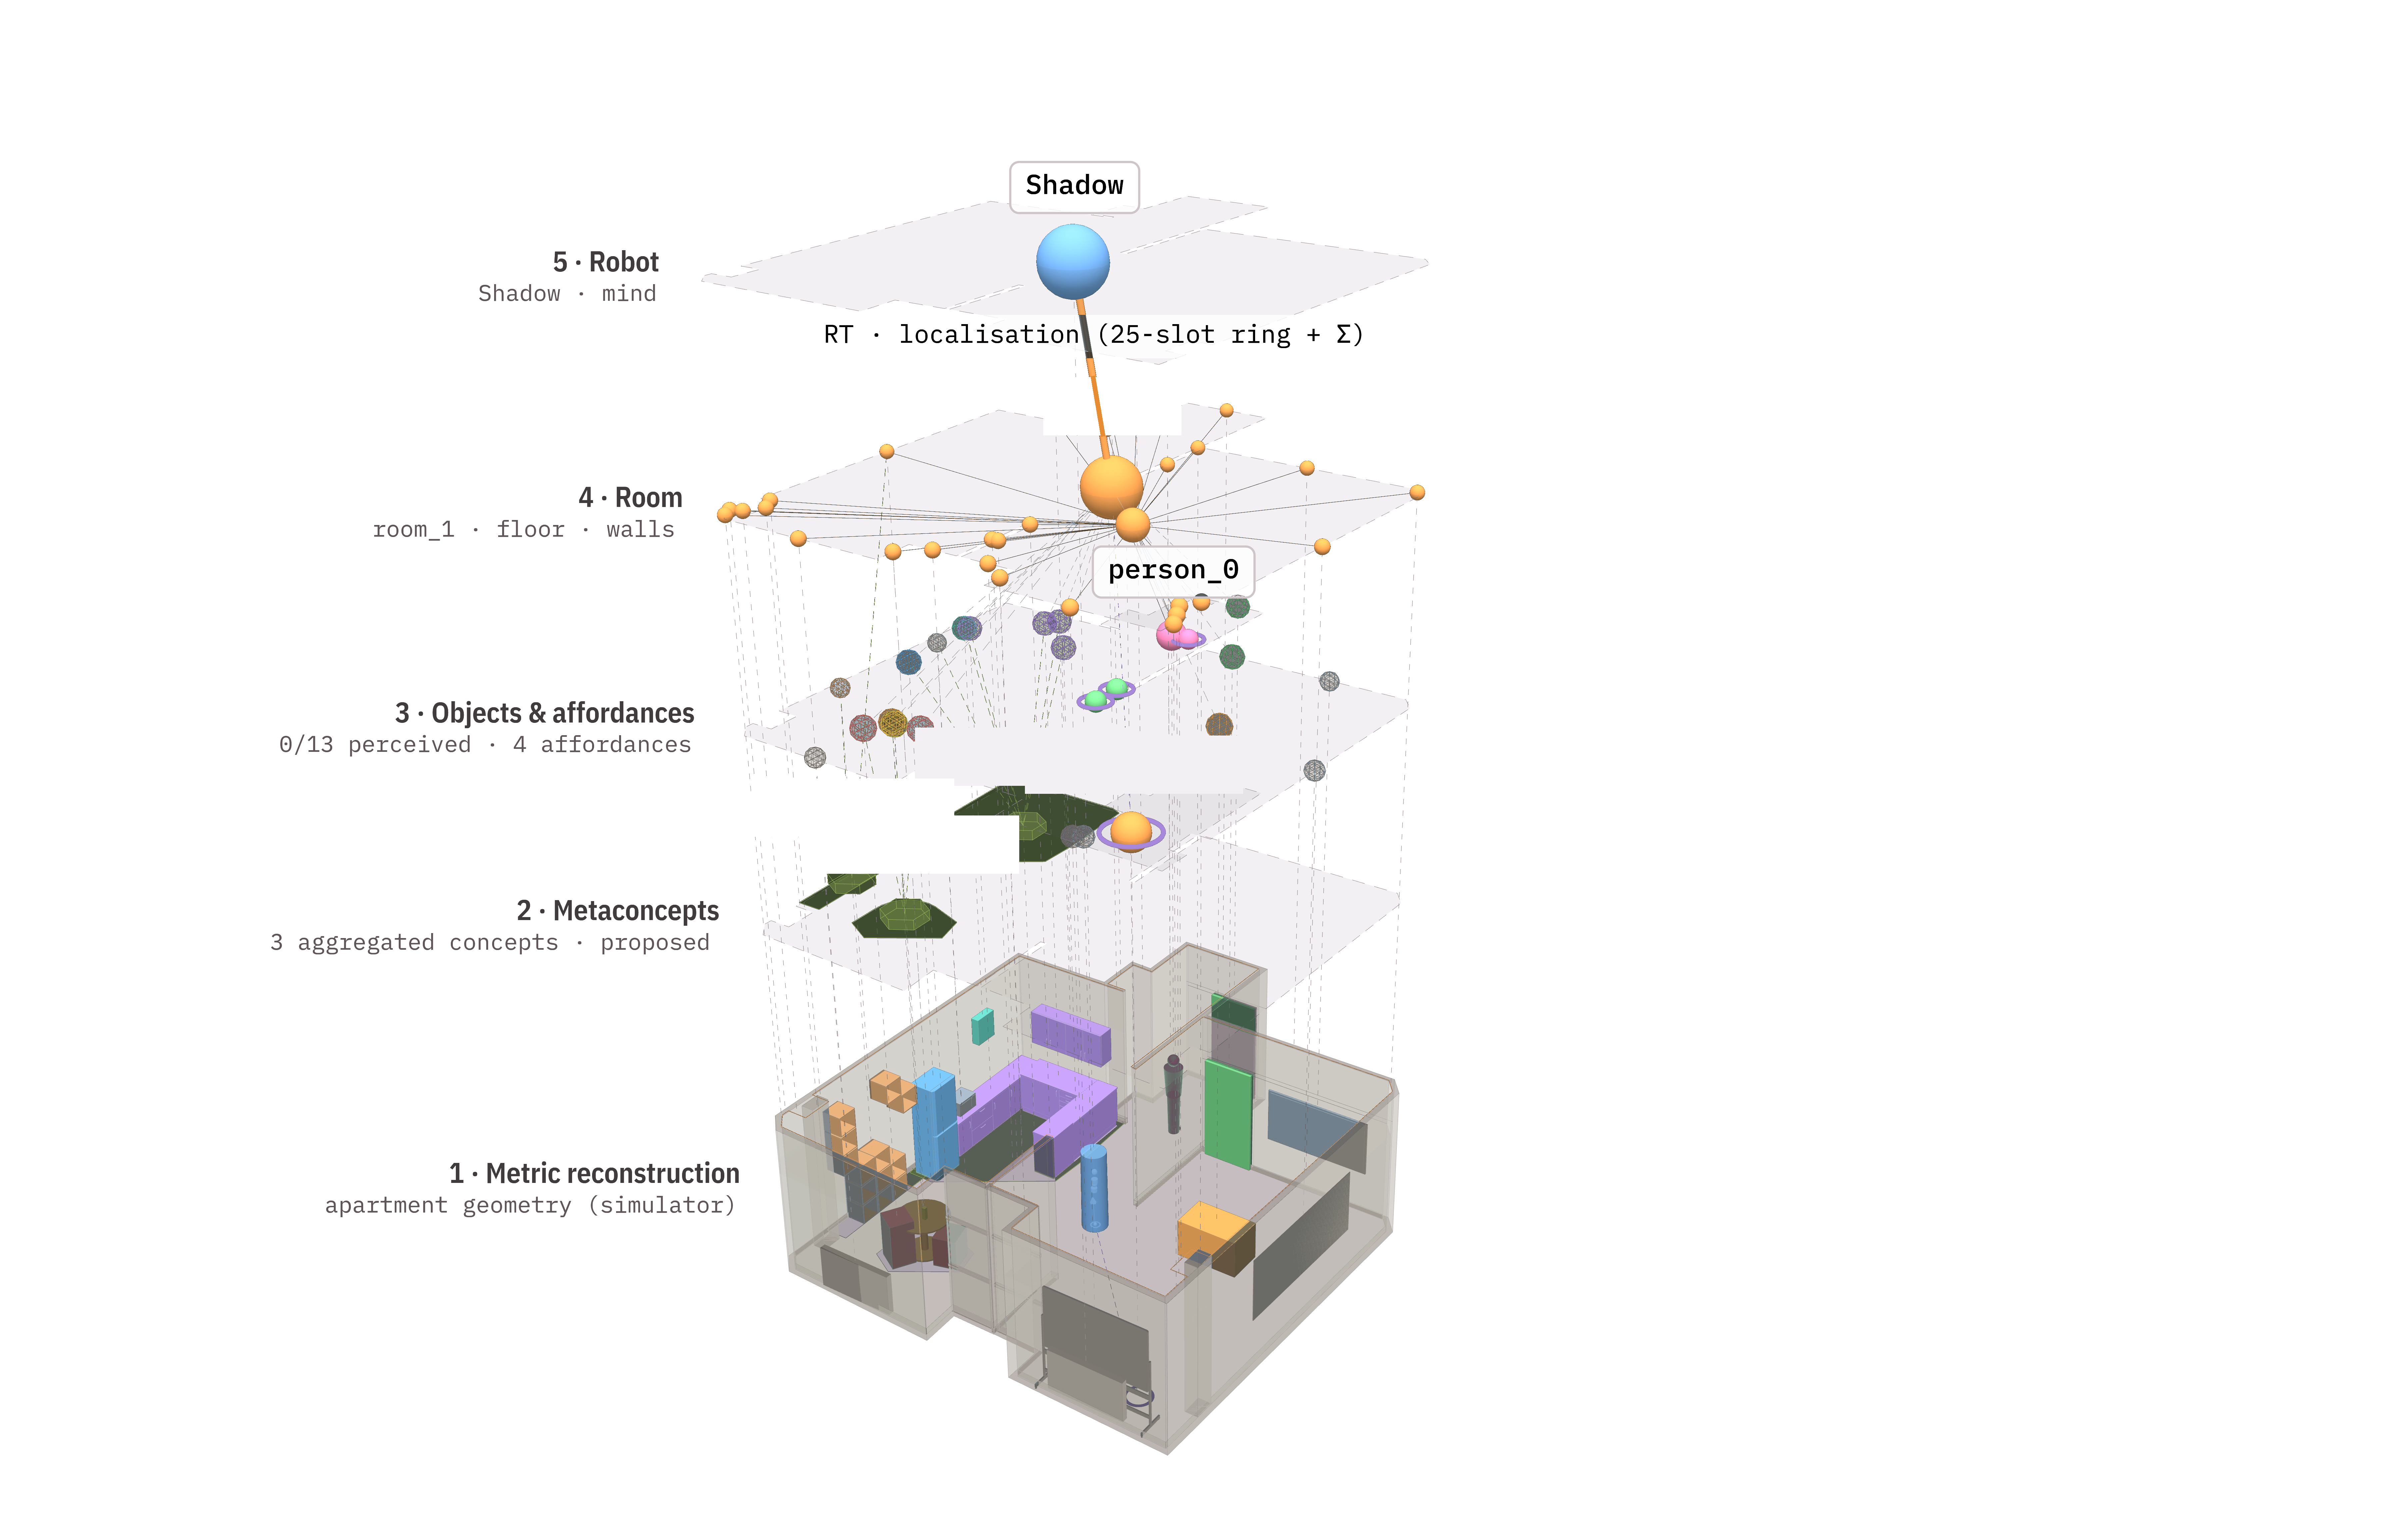
\includegraphics[width=\linewidth,trim=760 200 2850 420,clip]{figures/full_graph_white_clean.png}};
            \begin{scope}[x={(img.south east)}, y={(img.north west)}]
                % labels redrawn apart; the overlapping originals were removed from full_graph_white_clean.png
                \tikzset{lab/.style={draw=black!45, fill=white, rounded corners=1.5pt, inner sep=1.2pt,
                         font=\ttfamily\tiny}}
                \node[lab, anchor=east] at (0.690,0.800) {room\_1};
                \node[lab, anchor=west] at (0.425,0.505) {wall-shelf};
                \node[lab, anchor=west] at (0.470,0.462) {dinner-set};
                \node[lab, anchor=west] at (0.565,0.542) {kitchen-rig};
                \node[lab, anchor=west] at (0.775,0.515) {afford\_room};
                \fill[yellow!85!orange, draw=conceptc!80!black, thick] (0.80,0.585) circle (2.6pt);
                \node[draw=black!50, fill=white, rounded corners=1.5pt, inner sep=1.5pt,
                      font=\ttfamily\tiny, anchor=west] at (0.825,0.60) {chair\_34};
            \end{scope}
        \end{tikzpicture}
    \end{minipage}\hfill
    \begin{minipage}[c]{0.43\linewidth}
        \centering
        \resizebox{\linewidth}{!}{% belief-node.tex — schematic companion to Figure 2: one node of the graph as a belief.
% Uses the palette defined in vygotskian_machine_build.tex. Schematic, not data.
\begin{tikzpicture}[font=\scriptsize, >=Latex]
% ---------- the node card
\node[draw=conceptc, very thick, rounded corners=3pt, fill=conceptf, align=left, inner sep=4pt,
      text width=36mm, anchor=north west] (card) at (0,0) {%
  \tikz[baseline=-0.6ex]\fill[yellow!85!orange, draw=conceptc!80!black] (0,0) circle (2.4pt);\
  \textbf{\textcolor{conceptc!80!black}{chair\_34}}\\[1pt]
  owner: chair agent\\
  pose: mean $\mu$, covariance $\Sigma$\\
  existence: log-odds $\ell$\\
  parent: \texttt{room\_1}\\
  edge: transform $T$ and its $\Sigma$};
% ---------- floor sketch: pose belief seen from the robot
\begin{scope}[shift={(4.3,-2.15)}]
  \draw[black!55, thick] (0,0) -- (0,2.05) -- (3.0,2.05);
  \node[font=\tiny, text=black!55, anchor=south west] at (0,2.05) {room\_1 walls};
  % view cone
  \fill[wmc!25] (0.55,0.35) -- (2.75,1.65) -- (2.75,0.05) -- cycle;
  % robot
  \fill[bodyc!70] (0.55,0.35) circle (0.13);
  \draw[bodyc!80!black, thick, ->] (0.55,0.35) -- (0.9,0.55);
  \node[font=\tiny, text=bodyc!80!black, anchor=north] at (0.55,0.2) {robot};
  % chair belief: footprint at the mean, 2-sigma ellipse
  \draw[conceptc, thick, fill=conceptf, rotate around={25:(2.1,1.0)}] (2.1,1.0) ellipse (0.55 and 0.28);
  \draw[conceptc!80!black, fill=conceptc!45] (1.95,0.88) rectangle (2.25,1.12);
  \node[font=\tiny, text=conceptc!80!black, anchor=north] at (2.1,0.62) {$\mu$, $2\sigma$};
\end{scope}
% ---------- existence log-odds over time
\begin{scope}[shift={(0,-5.2)}]
  % segments
  \fill[wmc!18] (0.2,-0.75) rectangle (2.5,1.45);
  \fill[black!8] (2.5,-0.75) rectangle (4.6,1.45);
  \fill[bodyf] (4.6,-0.75) rectangle (7.0,1.45);
  \draw[->, black!60] (0,0) -- (7.35,0) node[anchor=west, font=\tiny, text=black!60] {time};
  \draw[->, black!60] (0,-0.75) -- (0,1.55) node[anchor=south, font=\tiny, text=black!60] {$\ell$};
  \draw[black!35, dashed] (0,0.0) -- (7.0,0.0);
  \draw[conceptc!85!black, very thick]
    (0.2,0.0) .. controls (0.9,0.7) and (1.6,1.05) .. (2.5,1.15)
    -- (4.6,1.15)
    .. controls (5.4,1.05) and (6.1,0.25) .. (6.9,-0.55);
  \node[font=\tiny, align=center, anchor=north] at (1.35,-0.78) {seen\\rises};
  \node[font=\tiny, align=center, anchor=north] at (3.55,-0.78) {occluded\\held};
  \node[font=\tiny, align=center, anchor=north] at (5.8,-0.78) {absent where\\detectable: falls};
\end{scope}
\end{tikzpicture}
}
    \end{minipage}
    \caption{Left: the output of \cortex{} in the simulated apartment, drawn by stratum: the robot (level~0),
    localised in \texttt{room\_1} (level~1); the objects and their affordances (level~2); and the aggregates fitted
    over them (level~3). The bottom stratum is the simulator's true geometry, shown for reference, and strata numbers
    give the drawing order, not the levels of Table~\ref{tab:lh_levels}. Right: a schematic of the node marked \texttt{chair\_34} on the left, as a belief
    owned by one agent, whose existence log-odds rises when the object is seen, is held while it is occluded, and
    falls only when it is absent where it could have been detected.}
    \label{fig:cortex_graph}
\end{figure}

\paragraph{Action and memory.}
A controller plans and follows paths. Its epistemic planner scores the actions that the concept agents offer, such as
looking at a door from a given place, by their expected free energy. An exploration drive turns this scoring into a
default behaviour. The robot explores the current room until further exploration yields too little information,
crosses the nearest uncrossed door, and returns in depth-first order. Three memory agents retain what the live graph
discards. The spatial memory stores each room the robot has left with the doors that connect it, and restores it as a
prior on return. The object memory keeps a persistent record of object instances. The episodic memory records the
robot's missions, their steps and how each ended. These memories provide the counts from which the priors and habits
of the Vygotskian machine will be learned.

\paragraph{The language agent.}
The language agent connects a person to all of these components through a vision-language model (VLM), Gemma 4
with 26 billion parameters, served by Ollama on an NVIDIA Jetson AGX Orin carried by the robot. Its design follows the principle
stated in the code as ``the model proposes, C++ decides''. The VLM sees a summary of the graph and the memories and can
act only by calling tools, and every call passes a deterministic gate that checks names against the graph and
arguments against the robot's capabilities. Extended behaviour is written in a small mission language (cross a door,
explore a room, approach an object, watch for a condition, if, repeat), and each mission is checked against the graph
and approved by the person before it runs. While a mission runs, robot events wake the model in restricted turns in
which it can look, query memory, stop and propose, but not act. Whether to ask the person or to make an assumption is
decided by a small rule over counts and costs. The agent also answers subjunctive questions with the robot's own
models, on an imagined copy of the room that can never write to the live graph. On that copy the controller answers
``would I fit?'', the perception models answer ``would I see it from there?'', and the episodic counts answer ``would
this route succeed?''. The imagination of Section~\ref{sec:lang_hierarchy:imagination} relies on these tools.

\paragraph{What is missing.}
\cortex{} can therefore perceive, hold beliefs, act, remember, talk and, when asked, imagine. Its VLM is used only when a
person speaks, nothing it knows becomes a prior, the robot never questions itself or imagines on its own initiative,
and the hundredth mission to the kitchen requires the same VLM calls as the first. The inner voice
(Section~\ref{sec:inner_speech}) and the cultural plane (Section~\ref{sec:lang_hierarchy}) address these gaps.

%     % =====================================================================================================
% vygotskian_internalisation.tex — The Vygotskian machine, part 2: internalisation (the inner voice)
%
% DRAFT (2026-11-19; first drafted 2026-11-18 as inner_speech_section.tex). A proposal section: it describes an
% architecture that is NOT yet implemented, grounded in the existing language_agent (robocomp/active_inference).
% Include from main.tex, in this order:
%     % =====================================================================================================
% vygotskian_machine.tex — The Vygotskian machine, part 1: the framing section
%
% DRAFT (2026-11-19). Opens the three-part proposal; a proposal, not a report of results.
% Include from main.tex, in this order:
%     % =====================================================================================================
% vygotskian_machine.tex — The Vygotskian machine, part 1: the framing section
%
% DRAFT (2026-11-19). Opens the three-part proposal; a proposal, not a report of results.
% Include from main.tex, in this order:
%     \input{vygotskian_machine}
%     \input{vygotskian_cortex}
%     \input{vygotskian_internalisation}
%     \input{vygotskian_cultural_plane}
%     \input{vygotskian_experiments}
% with \addbibresource{vygotskian_machine.bib} and \usepackage{array} in the preamble.
% =====================================================================================================

\section{The Vygotskian Machine}
\label{sec:vygotskian}

According to Vygotsky, higher mental functions develop in accordance with one central law: each function first
emerges in interactions between people, and then within the individual \cite{vygotsky1978mind}. A child plans aloud
together with an adult before planning aloud alone, plans aloud alone before planning silently, and plans silently
before the plan is carried out without any words at all. Language is what carries the child through this sequence. It
is the means by which knowledge held by other people becomes the learner's own, and it is also the tool with which the
learner regulates its own actions while that knowledge is still new.

We propose to build a robot that follows this law, and we call it a \emph{Vygotskian machine}. The robot's higher
functions, such as its goals, its plans, the meaning it gives to a scene and what it expects to find in a room, are
first provided from outside. They come from the person who lives with the robot and from a vision-language model (VLM),
a neural network trained on images and text that carries a large share of human culture. The robot then internalises
these functions, first as an inner voice that asks questions, makes plans and imagines outcomes
(Section~\ref{sec:inner_speech}), and eventually as prior beliefs, accumulated counts of experience and habits that
need no language at all. The robot's automatic level consists of the Active Inference agents that build its hierarchy
of beliefs and control its movement. This automatic level is what the internalised knowledge ultimately shapes, and
it is also the level that language is called upon to assist whenever the situation exceeds its competence.

\begin{table}[ht]
    \centering
    \small
    \begin{tabular}{|>{\raggedright\arraybackslash}p{0.4\linewidth}|>{\raggedright\arraybackslash}p{0.5\linewidth}|}
        \hline
        \textbf{Vygotsky} & \textbf{The machine} \\ \hline
        Every higher function emerges first between people, and then within the individual
            & goals, plans and scene meaning arrive as a person's words and the VLM's culture, then become priors,
              plans and habits (Sections~\ref{sec:lang_hierarchy:culture}--\ref{sec:lang_hierarchy:sequencing}) \\ \hline
        Outer speech $\to$ private speech $\to$ inner speech $\to$ no speech
            & the VLM writes a mission; the inner voice rehearses and monitors it; the compiled habit runs without
              language (Eq.~\ref{eq:lh_habit}) \\ \hline
        Private speech rises with task difficulty and fades with mastery \cite{berk1992children}
            & the demand signal recruits the voice on surprise and leaves it idle when the automatic level copes
              (Section~\ref{sec:inner_speech:modes}) \\ \hline
        Scaffolding by a more knowledgeable other, withdrawn as competence grows \cite{wood1976role}
            & the VLM's prior weight is overtaken by the robot's own counts (Eq.~\ref{eq:lh_beta_prior}); the person
              is asked less as experience accumulates \\ \hline
        The zone of proximal development: what the learner can do only with help
            & situations outside the automatic level's competence but within reach with the VLM or the person;
              learning moves them inside \\ \hline
        Mediation by signs: language as a psychological tool
            & the VLM's output is never accepted as belief; instead, it structures what the robot's own models do by
              proposing, sequencing and choosing what to imagine (Table~\ref{tab:lh_roles}) \\ \hline
    \end{tabular}
    \caption{Vygotsky's account and its counterpart in the proposed machine.}
    \label{tab:vygotskian_mapping}
\end{table}

\paragraph{Internalisation in Active Inference.}
Within the framework of this document, the passage from outer to inner speech can be given a precise
interpretation. Culture enters the generative model, the robot's probabilistic model of how its observations are
produced, in two places. It enters as prior beliefs and preferences, which describe what a room is for, which objects
tend to appear together and which outcomes are acceptable, and it enters as candidate policies, that is, sequences of
actions, which are scored by their expected free energy. Experience then internalises this culture in the two
corresponding places. The priors are progressively replaced by counts of what the robot itself has observed, and the
candidate policies that continue to succeed become part of the habit prior, a learned preference over policies. The
machine's dependence on language for routine matters should therefore decrease with experience, while remaining for
situations that are novel, social or structural.

\paragraph{Organisation.}
Section~\ref{sec:cortex} describes CORTEX, the architecture on which the machine is built. CORTEX already includes a
language agent, and the machine is defined by what it adds to that architecture. Section~\ref{sec:inner_speech}
develops internalisation. It treats the inner voice as an epistemic action, that is, an action taken to gain
information, and describes the attention modes that call on the voice and release it, as well as the learning that the
voice drives. Section~\ref{sec:lang_hierarchy} develops the cultural plane. It explains how the VLM is connected to the
belief hierarchy in three roles, namely culture, sequencing and imagination, under the rule that the language model
proposes and the generative models dispose.

\paragraph{The internalist contrast.}
According to the opposing, internalist view, language evolved first as an internal system for thought and was only
later used to communicate \cite{berwick2016why}. We use this view as a contrast rather than as a rival, because the
distinction it draws between the faculty of language and the content that language carries
(Section~\ref{sec:inner_speech:why_lm}) is what makes the Vygotskian claim testable. A machine that has a
compositional inner language but no culture serves as the \emph{non-Vygotskian control}. Its inner language is built
by library learning, the gradual collection of reusable sub-programmes, from the robot's own experience alone
(Section~\ref{sec:inner_speech:library}). If this control machine performs as well as the machine fed with culture in
situations far from anything the robot has seen, then culture is not doing the work that the name of the machine
claims for it.

\paragraph{Prior uses of the idea.}
Mirolli and Parisi argued for a Vygotskian cognitive robotics in which language serves as a cognitive tool as well as
a means of communication \cite{mirolli2011towards}, and Colas et al.\ proposed Vygotskian autotelic agents that
internalise language and culture to imagine and pursue their own goals \cite{colas2022language}. The present proposal
shares their premise but differs from them in three respects. First, internalisation is formalised within Active
Inference, as culture that enters priors and policies and gradually settles into counts and habits. Second, the
internalised knowledge acts on a probabilistic belief hierarchy whose evidence rules and cavity messages, which exclude
a belief's own contribution from the evidence it receives, prevent the hierarchy from confirming itself. Third, an
attention mechanism decides, from moment to moment, whether language is needed at all.

\paragraph{Two bitter lessons.}
Any proposal that builds knowledge into a robot has to respond to what Sutton called the bitter lesson. According to
Sutton, across seventy years of AI research, general methods that scale with computation, search and learning have
eventually outperformed methods that build in what their designers know \cite{sutton2019bitter}. Chess programs built
on human expertise were overtaken by search, and speech and vision systems built on expert-designed features were
overtaken by statistical learning. A robot whose levels 1 to 3 are generative models written by its designers, and
whose prior about kitchens is a table of log-odds written by hand, is open to the same criticism. A second lesson has
recently been drawn from the success of the first. Verbelen argues that ``the main idea behind modern AI is not
learning. It is amortisation'' \cite{verbelen2026newbitter}. In this view, training converts expensive inference into
reusable structure, so that a foundation model is a store of distilled past computation. Amortisation works when the
future resembles the past and fails when it does not. From this follows the new bitter lesson, that ``intelligence
cannot be fully amortised''. A system that must face a changing world needs, in addition to what it has precomputed,
three capabilities that amortisation does not supply, namely learning online during deployment, exploring actively to
reduce its own uncertainty, and forming new hypotheses when the old model no longer fits.

\paragraph{Where the Vygotskian machine stands.}
The two lessons pull in opposite directions. The first advises against handcrafting knowledge and in favour of using
what large-scale training has learned. The second warns that what large-scale training has learned is not enough, and
that a system must continue to perform inference. Neither lesson says how a system should combine the two, and such a
combination is what the Vygotskian machine proposes. Its novelty lies in four aspects.

\begin{enumerate}[(i)]
    \item \emph{Amortised culture as a proposal, never as a belief.} The VLM is the most amortised object
    available, since it contains human culture distilled by training at scale. The machine treats it as exactly
    that, the product of a general method, and uses it where Sutton's lesson says such methods should be used,
    namely to replace the hand-written parts of the system. The authored log-odds of the kitchen prior become priors
    elicited from the VLM, and the meaning of a room, which no designer has written down, also comes from the VLM.
    The machine never uses the VLM's output as its belief. Instead, the VLM's proposals are scored by ongoing
    inference against evidence, including evidence that something is absent, and they enter the generative model as
    pseudo-counts, imaginary prior observations that the robot's own experience gradually outweighs
    (Eq.~\eqref{eq:lh_beta_prior}).
    \item \emph{Internalisation is amortisation by the robot, with a way back.} The robot amortises its own
    ongoing inference, in the sense that what the inner voice works out in focused mode settles into priors, counts
    and habits that no longer need language. This process is the internalisation described by Vygotsky's law, and it
    is also the amortisation of the second lesson, carried out by the agent itself, on its own data, while it acts.
    Each compiled habit carries with it the assumptions under which it was learned
    (Section~\ref{sec:lang_hierarchy:sequencing}). When the probability of those assumptions falls, the habit is set
    aside and ongoing inference takes over again.
    \item \emph{A signal that decides when amortisation is enough.} The new bitter lesson states that
    amortisation fails when the situation is novel, but it does not say how an agent notices that this has happened.
    In the machine, this decision is made continuously by a demand signal, which is a prediction error weighted by
    its precision, that is, by the confidence placed in it (Section~\ref{sec:inner_speech:modes}). While the amortised
    levels predict well, the inner voice either remains silent or imagines, and a surprise calls on ongoing inference
    mediated by language. Private speech in children behaves in the same way, increasing with task difficulty and
    fading as the child gains mastery.
    \item \emph{The three missing properties, each with its own mechanism.} Online learning consists of the
    gradual replacement of the VLM's pseudo-counts by experience and the growth of the habit prior with experience.
    Active exploration takes the form of the inner question, treated as an epistemic action and scored by its
    expected information gain (Section~\ref{sec:inner_speech:questions}). New hypotheses arise from surprise at the
    level of the model itself. When the evidence for an arrangement of objects collapses, or when a class of objects
    repeatedly fails to fit where it is expected, the VLM proposes a new structure and the robot's own models test
    it. In every case, the VLM generates candidates and the robot's models evaluate them.
\end{enumerate}

The machine thus interprets the first lesson as a reason to take culture from a learned model instead of writing it
by hand, and the second as a reason to keep that culture outside the belief state, where ongoing inference can correct
it. Vygotsky's account supplies the developmental sequence that connects the two lessons, in which knowledge is first
borrowed from others, then used through speech, and finally internalised until it no longer needs speech.

\paragraph{What would demonstrate that the paper's goal has been achieved?}
The central claim rests on three predictions. First, the non-Vygotskian control falls behind the machine fed with
culture in proportion to the novelty of a situation (P7 in Section~\ref{sec:inner_speech:predictions}). Second, the
machine's use of language behaves as private speech does, increasing with difficulty and decreasing with mastery
(P8). Third, the scaffold provided by the VLM is withdrawn, so that as confirmed rooms and successful missions
accumulate, the number of calls to the VLM falls while task success is maintained (L6 in
Section~\ref{sec:lang_hierarchy:predictions}).

%     % =====================================================================================================
% vygotskian_cortex.tex — The Vygotskian machine, part 2: the CORTEX architecture it is built on
%
% DRAFT (2026-11-20, cut to budget). Describes what exists today, as a given resource. Descriptive, not a report
% of results: every component named here is in the robocomp/active_inference repository (ARCHITECTURE.md is the
% source). Include after vygotskian_machine.tex and before vygotskian_internalisation.tex.
% =====================================================================================================

\section{The Starting Point: the CORTEX Architecture}
\label{sec:cortex}

The Vygotskian machine is added to an existing and working robot architecture, \cortex{}, which runs on a mobile
robot called Shadow, both in a simulated apartment and in a real one. \cortex{} already builds a probabilistic model of
the robot's surroundings, acts on that model, remembers it, and talks about it with a person
through a language agent. We describe the architecture as it stands, because each proposal in the later sections is
defined by what it adds to these parts.

\input{figures/cortex-architecture-overview}

\paragraph{A shared graph of beliefs.}
At its core, \cortex{} is a shared, distributed and persistent scene graph, read and written concurrently by independent
processes called agents (Figure~\ref{fig:cortex_overview}, where the graph is drawn as the working memory). Agents
do not send messages to one another, and the graph
is the only interface through which they communicate. Each agent keeps a full replica, and the replicas are merged as
conflict-free replicated data types, whose copies converge to the same state without coordination. Geometric edges
hold a rigid transform with its covariance, and they form a tree from the world through the rooms to the objects, and
from the robot's base to its sensors. An agent is a process that maintains a probabilistic belief over one kind of
entity and publishes it with its mean and covariance. Other agents treat this posterior as evidence weighted by its
covariance, and never as ground truth. Effects that a conventional system would express as a threshold, such as
ignoring distant detections, are instead written into the generative model, usually as a covariance that grows with a
physical quantity. The thresholds that this paper does introduce are declared, with their justification, in
Section~\ref{sec:inner_speech:modes}.

\paragraph{A probabilistic hierarchy.}
The beliefs in the graph form a hierarchy of five levels (Table~\ref{tab:lh_levels}), namely the robot itself, its
rooms, the objects in those rooms, aggregates of objects, and cultural abstractions such as what a room is for. Each
level is expressed in the frame of the level below, its measurements are the posteriors published by that level, and
it can send back down an empirical prior, that is, a message stating what it expects its parts to be. The first four
levels constitute \cortex{} as it exists, and they are built automatically and without language. The fifth is the
addition made in this paper. Figure~\ref{fig:cortex_graph} shows the graph that \cortex{} builds in the simulated
apartment.

\begin{table}[ht]
    \centering
    \small
    \begin{tabular}{|>{\raggedright\arraybackslash}p{0.05\linewidth}|>{\raggedright\arraybackslash}p{0.16\linewidth}|>{\raggedright\arraybackslash}p{0.33\linewidth}|>{\raggedright\arraybackslash}p{0.17\linewidth}|>{\raggedright\arraybackslash}p{0.13\linewidth}|}
        \hline
        \textbf{Level} & \textbf{What} & \textbf{Latent} & \textbf{Source of its model} & \textbf{Status} \\ \hline
        0 & robot (self) & body, sensor mounts, pose & calibration, self-calibration & implemented \\ \hline
        1 & room(s) & layout of each room, the robot's place in it, the doors that join rooms & authored generative model, fitted online; spatial memory & implemented \\ \hline
        2 & objects & per instance: class, pose, extent, existence & authored generative models, fitted online & implemented \\ \hline
        3 & metaconcepts (aggregates) & arrangements: a ring of chairs around a table, the rectilinear frame of a kitchen & authored schemas & implemented (the kitchen's priors not yet sent down) \\ \hline
        4 & cultural abstraction & the function of a room (kitchen, dining, bedroom, \ldots) & \textbf{culture: the VLM}, weighted by measured reliability and replaced by counts & \textbf{added by this paper} (Section~\ref{sec:lang_hierarchy:culture}) \\ \hline
    \end{tabular}
    \caption{The probabilistic belief hierarchy. Levels 0--3 are \cortex{} as it exists, and level 4 is added here.}
    \label{tab:lh_levels}
\end{table}



\paragraph{Levels 0 to 3.}
At level 0, an agent dedicated to the body maintains the tree of frames from the base to each sensor, and a
self-calibration agent estimates where each sensor is mounted, so that these transforms are themselves beliefs. At
level 1, a room agent jointly estimates the layout of the current room and the robot's location in it, and decides
from evidence whether the robot has entered a new room or returned to a known one. Rooms are joined by doors, and the
robot's world is a graph of rooms of which only one is actively estimated at a time. At level 2, each class of object
has its own concept agent, for tables, chairs, cabinets, refrigerators, doors, beds, people and others. Each agent
tracks instances from segmentation masks and depth, updates a class-specific generative model with a shared recursive
variational Laplace engine, and publishes each instance in the frame of its room. A residual agent models the
occupancy that no other agent explains, and acts as the null hypothesis of the scene. Every instance carries an
existence log-odds, raised by evidence that was predicted and observed and lowered by evidence that was predicted but
absent, only where the object could have been detected, so that an occluded object is retained rather than refuted.
At level 3, two metaconcepts fit aggregates, a table with its ring of chairs and the frame shared by the units of a
kitchen. The existence of an aggregate is a log Bayes factor against an explicit null of independent objects, and
each aggregate sends empirical priors to its members, computed without that member's own contribution
(Eq.~\eqref{eq:lh_cavity}). Level 4, the purpose of a room and how the robot should behave there, is not represented
in \cortex{} and is the contribution of this paper (Section~\ref{sec:lang_hierarchy:culture}).



\begin{figure}[!h]
    \centering
    \begin{minipage}[c]{0.53\linewidth}
        \centering
        \begin{tikzpicture}
            \node[anchor=south west, inner sep=0] (img) at (0,0)
                {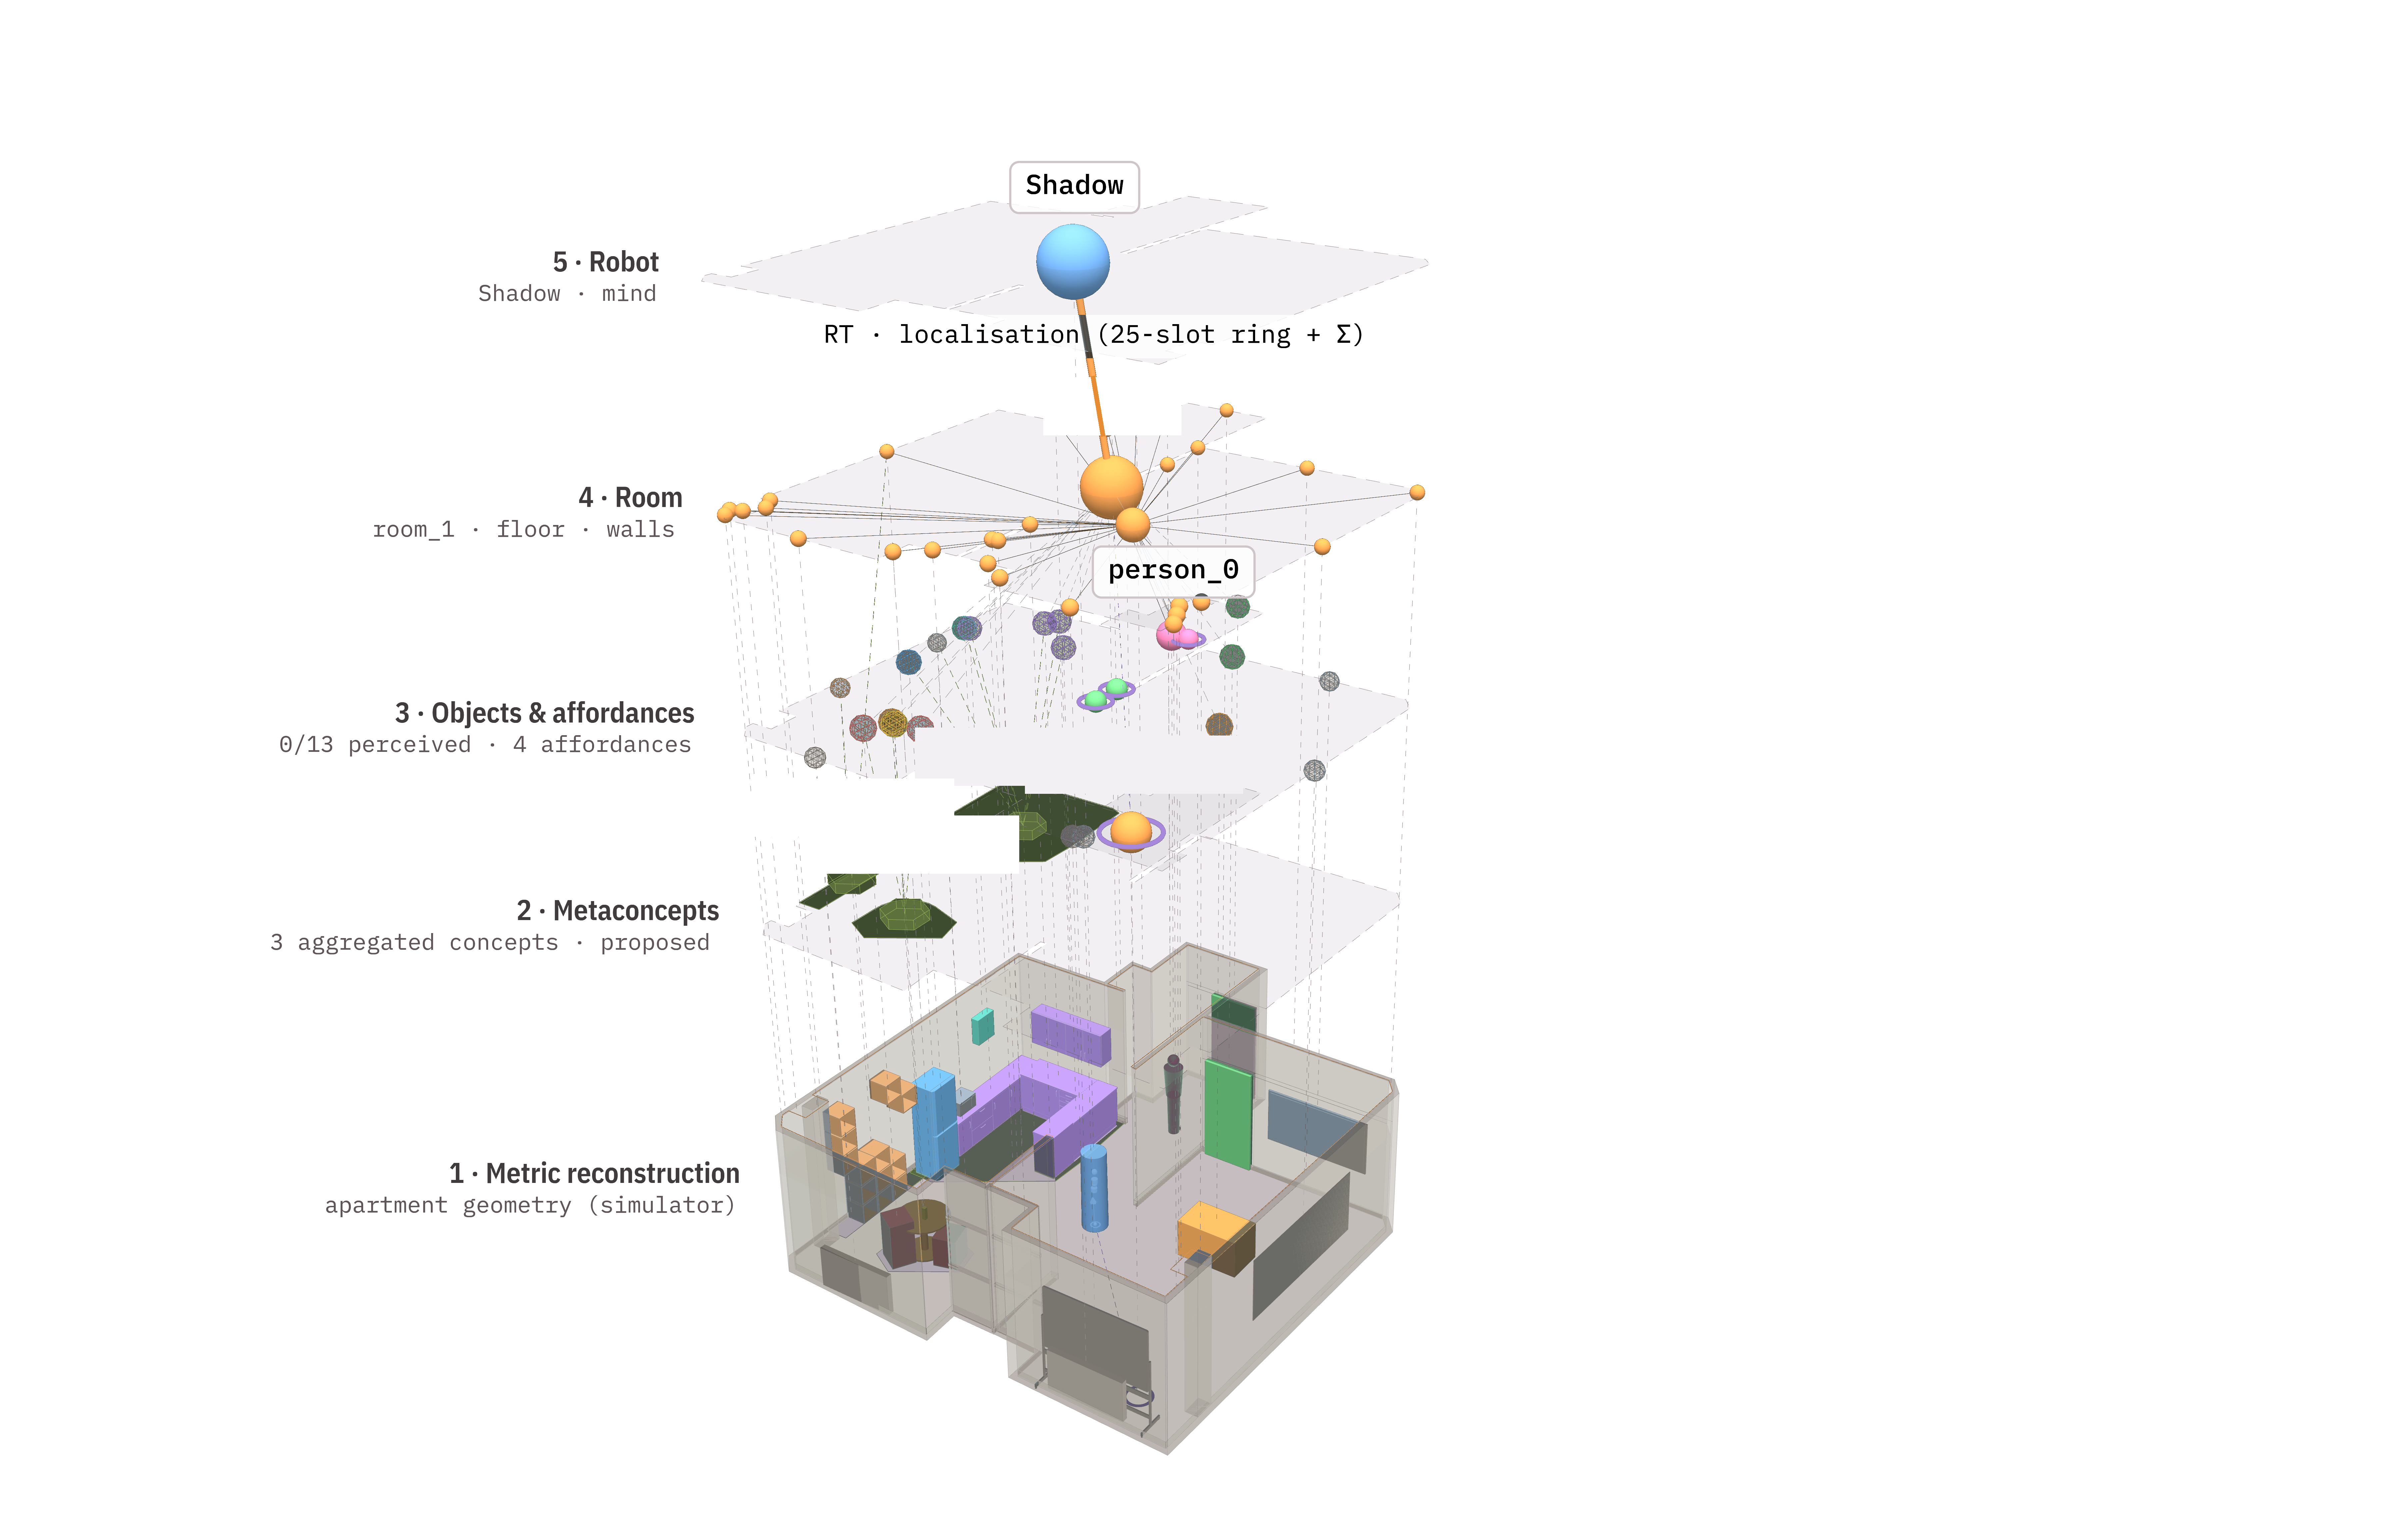
\includegraphics[width=\linewidth,trim=760 200 2850 420,clip]{figures/full_graph_white_clean.png}};
            \begin{scope}[x={(img.south east)}, y={(img.north west)}]
                % labels redrawn apart; the overlapping originals were removed from full_graph_white_clean.png
                \tikzset{lab/.style={draw=black!45, fill=white, rounded corners=1.5pt, inner sep=1.2pt,
                         font=\ttfamily\tiny}}
                \node[lab, anchor=east] at (0.690,0.800) {room\_1};
                \node[lab, anchor=west] at (0.425,0.505) {wall-shelf};
                \node[lab, anchor=west] at (0.470,0.462) {dinner-set};
                \node[lab, anchor=west] at (0.565,0.542) {kitchen-rig};
                \node[lab, anchor=west] at (0.775,0.515) {afford\_room};
                \fill[yellow!85!orange, draw=conceptc!80!black, thick] (0.80,0.585) circle (2.6pt);
                \node[draw=black!50, fill=white, rounded corners=1.5pt, inner sep=1.5pt,
                      font=\ttfamily\tiny, anchor=west] at (0.825,0.60) {chair\_34};
            \end{scope}
        \end{tikzpicture}
    \end{minipage}\hfill
    \begin{minipage}[c]{0.43\linewidth}
        \centering
        \resizebox{\linewidth}{!}{\input{figures/belief-node}}
    \end{minipage}
    \caption{Left: the output of \cortex{} in the simulated apartment, drawn by stratum: the robot (level~0),
    localised in \texttt{room\_1} (level~1); the objects and their affordances (level~2); and the aggregates fitted
    over them (level~3). The bottom stratum is the simulator's true geometry, shown for reference, and strata numbers
    give the drawing order, not the levels of Table~\ref{tab:lh_levels}. Right: a schematic of the node marked \texttt{chair\_34} on the left, as a belief
    owned by one agent, whose existence log-odds rises when the object is seen, is held while it is occluded, and
    falls only when it is absent where it could have been detected.}
    \label{fig:cortex_graph}
\end{figure}

\paragraph{Action and memory.}
A controller plans and follows paths. Its epistemic planner scores the actions that the concept agents offer, such as
looking at a door from a given place, by their expected free energy. An exploration drive turns this scoring into a
default behaviour. The robot explores the current room until further exploration yields too little information,
crosses the nearest uncrossed door, and returns in depth-first order. Three memory agents retain what the live graph
discards. The spatial memory stores each room the robot has left with the doors that connect it, and restores it as a
prior on return. The object memory keeps a persistent record of object instances. The episodic memory records the
robot's missions, their steps and how each ended. These memories provide the counts from which the priors and habits
of the Vygotskian machine will be learned.

\paragraph{The language agent.}
The language agent connects a person to all of these components through a vision-language model (VLM), Gemma 4
with 26 billion parameters, served by Ollama on an NVIDIA Jetson AGX Orin carried by the robot. Its design follows the principle
stated in the code as ``the model proposes, C++ decides''. The VLM sees a summary of the graph and the memories and can
act only by calling tools, and every call passes a deterministic gate that checks names against the graph and
arguments against the robot's capabilities. Extended behaviour is written in a small mission language (cross a door,
explore a room, approach an object, watch for a condition, if, repeat), and each mission is checked against the graph
and approved by the person before it runs. While a mission runs, robot events wake the model in restricted turns in
which it can look, query memory, stop and propose, but not act. Whether to ask the person or to make an assumption is
decided by a small rule over counts and costs. The agent also answers subjunctive questions with the robot's own
models, on an imagined copy of the room that can never write to the live graph. On that copy the controller answers
``would I fit?'', the perception models answer ``would I see it from there?'', and the episodic counts answer ``would
this route succeed?''. The imagination of Section~\ref{sec:lang_hierarchy:imagination} relies on these tools.

\paragraph{What is missing.}
\cortex{} can therefore perceive, hold beliefs, act, remember, talk and, when asked, imagine. Its VLM is used only when a
person speaks, nothing it knows becomes a prior, the robot never questions itself or imagines on its own initiative,
and the hundredth mission to the kitchen requires the same VLM calls as the first. The inner voice
(Section~\ref{sec:inner_speech}) and the cultural plane (Section~\ref{sec:lang_hierarchy}) address these gaps.

%     % =====================================================================================================
% vygotskian_internalisation.tex — The Vygotskian machine, part 2: internalisation (the inner voice)
%
% DRAFT (2026-11-19; first drafted 2026-11-18 as inner_speech_section.tex). A proposal section: it describes an
% architecture that is NOT yet implemented, grounded in the existing language_agent (robocomp/active_inference).
% Include from main.tex, in this order:
%     \input{vygotskian_machine}
%     \input{vygotskian_internalisation}
%     \input{vygotskian_cultural_plane}
% and add the shared bibliography:  \addbibresource{vygotskian_machine.bib}
% Packages used: amsmath, amssymb, enumitem (already loaded by main.tex) and array, which main.tex does not
% load yet: add \usepackage{array} to its preamble.
% Labels keep their original sec:inner_speech:* prefix so that existing cross-references do not break.
% =====================================================================================================

\section{Internalisation: the Inner Voice}
\label{sec:inner_speech}

The robot described so far uses language in one direction only: a person speaks, and a language agent turns
the request into commands for the controller, grounded in a textual digest of the belief graph. This section
proposes to turn that capability inward, which constitutes the internalisation step of the Vygotskian machine
(Section~\ref{sec:vygotskian}). We argue that a language model embedded in an Active Inference
architecture can play the role that inner speech plays in human cognition, namely that of a serial and
compositional medium in which the agent poses questions to itself, generates hypotheses, rehearses plans and
replays its past. We further argue that this role follows naturally from the epistemic component of expected free
energy. The proposal is presented together with the constraints that prevent such a voice from becoming a source
of confabulated beliefs, and with the experiments that would falsify it.

\subsection{Motivation: from talk to thought}
\label{sec:inner_speech:motivation}

Two theoretical traditions disagree about the origin of inner speech, but they agree about its function. According
to the developmental view that gives the machine its name, inner speech is social speech that the child gradually internalises, abbreviates and
turns into a tool for self-regulation \cite{vygotsky1986thought}. According to the internalist view, which we use
as the point of contrast throughout this section, human language evolved first as an internal system for structuring thought, and its use for
communication is a later externalisation \cite{berwick2016why}. Contemporary reviews treat inner speech as
functionally involved in planning, problem solving, self-monitoring and the maintenance of goals in working memory
\cite{aldersonday2015inner}, and language more generally as a cognitive technology that lets a learner manipulate
discrete, recombinable tokens rather than raw percepts \cite{clark1998magic}.

Large language models provide a striking example of the developmental route. They are trained exclusively on
communicative text, yet their performance improves measurably when they produce intermediate reasoning in that
same medium before answering, a technique known as chain-of-thought \cite{wei2022chain}. In this sense, a system
built for communication becomes better at reasoning when it addresses its speech to itself. Our language agent is
at a comparable point in its own development. It was built to converse with a person, and the question we ask is
what it contributes once its speech is addressed to the robot itself.
Section~\ref{sec:inner_speech:why_lm} returns to the internalist contrast, and Section~\ref{sec:inner_speech:library}
turns it into a control experiment.

\subsection{Inner questions as epistemic actions}
\label{sec:inner_speech:questions}

In Active Inference, policies are scored by expected free energy, whose epistemic term rewards the expected
reduction of uncertainty about hidden states \cite{friston2017process, parr2022active}. A question can be
regarded as the linguistic expression of exactly this quantity, since it names a hidden variable whose value is
uncertain and whose resolution is expected to matter. We therefore model an inner question as a persistent object
\begin{equation}
    \mathcal{Q} = \big\langle\, e,\; \mathcal{H},\; q(h),\; \mathcal{P},\; b,\; s \,\big\rangle ,
    \label{eq:inner_question}
\end{equation}
where $e$ is the triggering event (for example an obstacle no concept agent explains), $\mathcal{H}$ a finite set
of named hypotheses (``a chair'', ``a box'', ``unknown''), $q(h)$ the current posterior over them, $\mathcal{P}$
the set of pending predictions, $b$ a budget in time and motion, and $s \in \{\text{open},\text{resolved},
\text{abandoned}\}$ its status. Questions are organised as a stack, in the sense of a \emph{question under
discussion} \cite{roberts2012information}, so that ``is it a chair?'' is a sub-question whose answer partially
resolves the parent question ``what is this?''. It is the question object, and not the language model's context
window, that carries the state of the reasoning from one step to the next.

\paragraph{One step of the loop.}
Given $\mathcal{Q}$, the language model proposes a test, which consists of an epistemic action $a$ (turning
towards the anomaly, approaching it, looking with the front camera) together with the outcome that each hypothesis
predicts. The value of the test
is its expected information gain minus its cost,
\begin{equation}
    V(a) \;=\; \underbrace{H\!\left[q(h)\right] \;-\; \mathbb{E}_{p(o \mid a)}\!\left[ H\!\left[q(h \mid o, a)\right]
    \right]}_{I(h;\,o \mid a)} \;-\; c(a),
    \label{eq:inner_value}
\end{equation}
which is the negative of the epistemic part of expected free energy with an explicit action cost. The test is
executed only if $V(a) > 0$ and the action passes the same deterministic gate that already validates every
command the language agent issues. When the observation $o$ arrives, the posterior is updated by the concept
agents' own likelihoods,
\begin{equation}
    q(h \mid o, a) \;\propto\; p(o \mid h, a)\, q(h),
    \label{eq:inner_update}
\end{equation}
and the loop continues, spawns a sub-question, or terminates when
\begin{equation}
    H\!\left[q(h)\right] < \eta \quad\lor\quad \max_a V(a) \le 0 \quad\lor\quad b \text{ exhausted}.
    \label{eq:inner_stop}
\end{equation}
This stopping rule is what distinguishes reasoning from rumination. A loop with no expected information left to
gain is closed, possibly with the answer ``unknown'', and the event that triggered it is habituated, that is,
ignored for a refractory period.

\paragraph{The grounding constraint.}
The central design rule is that the language model may suggest hypotheses but only perception may decide between
them; in short, \emph{the language model proposes and perception disposes}. Text produced by the model may
introduce hypotheses, predictions and tests, but it may never change a posterior. Only the likelihood
$p(o \mid h, a)$ in \eqref{eq:inner_update}, computed by the perceptual agents from sensor data, can do so. This
rule is the counterpart, on the side of beliefs, of the rule that the language agent already enforces for actions,
under which every proposed command is validated in C++ against the belief graph before it reaches the controller.
Without it, a language loop addressed to itself would be a closed system in which text is conditioned only on
text, and it would converge on its own confabulations.

\paragraph{The proposer as a calibrated prior.}
The hypotheses the model names, and the probabilities it attaches to them, encode world knowledge the robot has
not acquired by itself (``chairs come with tables''). We treat this knowledge as a prior whose weight must be
earned through demonstrated accuracy. Let
$\pi_{\text{LM}}(h \mid x)$ be the proposer's distribution in context $x$ and $n_x(h)$ the robot's own counts of
resolved questions in that context. The prior entering \eqref{eq:inner_update} is
\begin{equation}
    q_0(h \mid x) \;\propto\; \pi_{\text{LM}}(h \mid x)^{\beta_x}\, \big(\alpha + n_x(h)\big),
    \label{eq:inner_prior}
\end{equation}
a tempered product of the proposer and a Dirichlet over experience, where $\beta_x \in [0,1]$ is set from the
proposer's measured calibration in that context (for instance from its Brier score on past questions). Early in
the robot's life the proposer dominates this prior, and as the counts accumulate, the robot's own experience
progressively replaces the knowledge borrowed from the language model. The same conjugate form already governs the language agent's decision to ask a person or to assume
that they moved an object, where a Beta posterior over the person's past answers is compared against the costs of
asking and of being wrong.

\subsection{Attention, automaticity and the wandering mind}
\label{sec:inner_speech:modes}

A human driver on an easy road can steer without attending to the road, which leaves the mind free to plan, imagine
or recall, and attention returns to the task as soon as something unexpected happens
\cite{smallwood2015science, christoff2016mind}. In Active Inference this phenomenon is described in terms of
precision. While prediction errors are small and the habitual policy is reliable, attention, understood as the
precision assigned to sensory prediction errors, can be withdrawn from the task, and a surprise raises it again
\cite{feldman2010attention}. The account in which habitual and deliberative control are arbitrated according to
their relative uncertainty \cite{daw2005uncertainty} has the same structure.

The architecture already separates the two systems. The controller and the concept agents form an automatic layer
that drives, avoids obstacles and executes missions without the language model, while the language agent provides
the deliberative voice. We propose to make the allocation of this voice explicit through a scalar \emph{demand}
signal, computed without the language model each time the textual digest of the belief graph is updated,
\begin{equation}
    D_t \;=\; \sum_{k} \pi_k\, \varepsilon_{k,t}^{2} \;+\; \lambda\, \mathbb{1}\!\left[\text{person active}_t\right],
    \label{eq:inner_demand}
\end{equation}
where $\varepsilon_{k,t}$ are normalised prediction errors reported by the agents (unexplained residual occupancy,
flips of existence or door beliefs, localisation uncertainty, stalled or failed mission steps, controller refusals)
and $\pi_k$ their precisions. Three operating modes then follow from two thresholds with asymmetric hysteresis:
\begin{equation}
    m_t =
    \begin{cases}
        \textsc{focused}    & D_t > \theta_{\text{hi}},\\[2pt]
        \textsc{wandering}  & D_\tau < \theta_{\text{lo}} \;\; \forall\, \tau \in [t - T, t],\\[2pt]
        \textsc{monitoring} & \text{otherwise.}
    \end{cases}
    \label{eq:inner_modes}
\end{equation}
Entering \textsc{wandering} requires demand to stay low for a dwell time $T$; leaving it requires a single sample
above $\theta_{\text{hi}}$. The robot is therefore slow to let its attention drift away from the task and
immediate in returning to it. Safety never depends on this arbitration, because the controller's reflexes act on
their own and the deliberative voice engages only after the reflex has acted, just as a driver becomes aware of a
hazard only after having braked.

\paragraph{Focused mode} runs the question loop of Section~\ref{sec:inner_speech:questions} on the triggering
event. \paragraph{Monitoring mode} makes no calls to the language model, so that the voice is ready to engage but
remains silent.

\paragraph{Wandering mode.}
When the voice is freed from the task, it is seeded with one recent experience chosen by salience, such as an
episode that ended unresolved, a failure, an object that changed, or an upcoming goal. The output of each step,
together with an associative retrieval from episodic memory, seeds the next step, so that the chain of thoughts
drifts in the way spontaneous thought does \cite{christoff2016mind}. The voice has access only to memory queries and to the architecture's imagination tools,
which simulate observations and outcomes on a copy of the belief graph; it can neither act nor write beliefs. Its
products are of three kinds: counterfactuals over past episodes (``had the door been open, the crossing would have
taken 40\,s less''), hypotheses to be tested later, and prospective plans (``if the door is shut on the way back,
the route through the next room is shorter''). Functionally, this corresponds to the role of the brain's default
network in simulating the past and the future \cite{buckner2008brain}, and to the offline replay and model reduction that Active Inference assigns
to rest and sleep \cite{friston2017curiosity, hobson2012waking}. Replay is prioritised by the expected gain of the
memory it revisits \cite{mattar2018prioritized}.

\paragraph{Source monitoring.}
Humans occasionally misremember imagined events as perceived ones \cite{johnson1993source}, and the robot must not
make this error.
Everything produced while wandering is stored with an \emph{imagined} provenance, separate from the factual
episodic record, and enters the learning loop only as a hypothesis to be tested, never as evidence.

\subsection{What the return to reality gives the automatic layer}
\label{sec:inner_speech:return}

The transition from \textsc{wandering} to \textsc{focused} cancels the chain of thought in progress (its state is
kept, so that it may resume if demand subsides) and devotes the voice entirely to the surprising event. This return
to reality serves the automatic layer on three timescales.
\begin{enumerate}
    \item \textbf{Decision.} A surprise indicates that the automatic layer has left its domain of competence, and
    outside that domain its only responses are to retry, to stop or to fail. The voice adds the re-interpretation of
    the scene, arbitration between goals, re-planning through the remembered topology, and recourse to a person.
    \item \textbf{Attention.} The voice can raise precision where it matters, by orienting sensors, increasing a
    detector's rate in a region, or passing a hypothesis to the concept agents as a spatial prior. Such a prior has
    bounded weight, so that it may accelerate the recognition of an object that is present but cannot create one
    that is absent, which preserves the grounding constraint.
    \item \textbf{Teaching.} Each resolved surprise is a labelled example that the automatic layer could not have
    produced alone. For instance, an unexplained residual later identified as a chair is a false negative of the
    chair detector, a door that is repeatedly shut in the evening becomes a prior, and a recovery that repeatedly
    succeeds becomes a branch of the controller's behaviour tree. In this way the domain of competence grows and the
    situations that require the voice become rarer, which is the classical progression from effortful to autonomous
    skill \cite{fitts1967human}.
\end{enumerate}
Plans prepared while wandering act as a store of precomputed solutions, so that when the anticipated situation
occurs, the focused voice verifies an existing plan instead of composing a new one. The return ends with an
explicit release, in which spatial priors are cleared, safety margins are restored and the automatic layer is
confirmed to be back within its competence. Without this release, every surprise would leave the robot permanently
vigilant.

\subsection{Relation to chain-of-thought reasoning}
\label{sec:inner_speech:cot}

Chain-of-thought reasoning is a form of inner speech in the functional sense, although of a specific kind, and
comparing the two clarifies the design (Table~\ref{tab:inner_cot}). Plain chain-of-thought is convergent and
ungrounded, in that each token is conditioned only on previous tokens until an answer is produced, after which the
trace is discarded. Reasoning becomes grounded when it is interleaved with action and observation
\cite{yao2023react}. Our focused loop is of this kind, with the additional property that the observation, through
\eqref{eq:inner_update}, rather than the next token, determines the direction the reasoning takes. The wandering
voice is closer to plain chain-of-thought in its isolation from perception, but it is divergent rather than
convergent, it can be interrupted, and its products persist.

\begin{table}[ht]
    \centering
    \small
    \begin{tabular}{|>{\raggedright\arraybackslash}p{0.19\linewidth}|>{\raggedright\arraybackslash}p{0.22\linewidth}|>{\raggedright\arraybackslash}p{0.24\linewidth}|>{\raggedright\arraybackslash}p{0.24\linewidth}|}
        \hline
                                & \textbf{Chain-of-thought} & \textbf{Focused voice} & \textbf{Wandering voice} \\ \hline
        Goal                    & answer a given question   & resolve a given surprise & none given; seeded by salience \\ \hline
        Dynamics                & convergent                & convergent             & divergent, associative \\ \hline
        Contact with the world  & none                      & thought--action--observation & none (imagination only) \\ \hline
        Persistence             & discarded                 & question objects, beliefs, lessons & imagined store, hypotheses \\ \hline
        Interruptible           & no                        & yes                    & yes, resumable \\ \hline
        Latency budget          & n/a                       & $\sim$1\,s, no extended thinking & unbounded, extended thinking \\ \hline
    \end{tabular}
    \caption{Chain-of-thought compared with the two modes of the proposed inner voice.}
    \label{tab:inner_cot}
\end{table}

Two practical consequences follow. First, extended reasoning should take place \emph{when there is time, not when
there is pressure}. In the deployed language agent the model's extended thinking is disabled, because a model
operating in thinking mode spent 3\,000--6\,000 tokens (40--80\,s) before each tool call. Such a delay is
incompatible with the focused mode but costs nothing in the wandering mode, where extended thinking can be enabled
with a large budget and pre-empted at any moment. In this way slow reasoning is carried out in advance, and fast
reasoning makes use of its results. Second, chain-of-thought traces are known not always to reflect the
computation that produced the answer \cite{turpin2023language}, as human verbal reports do not always reflect the
causes of behaviour \cite{nisbett1977telling}. The faithful record of the robot's reasoning is therefore the
structured record of hypotheses, predictions, observations and posterior updates, not the generated text. Finally,
wandering chains whose hypotheses were later confirmed by perception form a corpus of reasoning verified against the world,
which could be used to fine-tune the local model in the manner of self-taught reasoning \cite{zelikman2022star},
with perception, rather than a known answer, as the filter.

\subsection{Consequences for belief and learning}
\label{sec:inner_speech:learning}

The question loop changes the way beliefs evolve in two respects. Within an episode, uncertainty is reduced where surprise
occurred rather than where the sensors happened to point, which is efficient but leaves the rest of the map less
examined and makes the robot's own data a biased sample; a decaying novelty term \cite{schwartenbeck2019curiosity}
and importance weighting of learned statistics are required to correct this. Across episodes, every closed
question is a labelled example, and learning proceeds at four timescales (Table~\ref{tab:inner_learning}).

\begin{table}[ht]
    \centering
    \small
    \begin{tabular}{|>{\raggedright\arraybackslash}p{0.14\linewidth}|>{\raggedright\arraybackslash}p{0.37\linewidth}|>{\raggedright\arraybackslash}p{0.37\linewidth}|}
        \hline
        \textbf{Timescale} & \textbf{What changes} & \textbf{Where, in this architecture} \\ \hline
        Seconds   & posterior over the hypotheses of one question         & the question object \eqref{eq:inner_question} \\ \hline
        Days      & priors: where objects are, which doors are shut, what moves & long-term object and topological memory, as Dirichlet counts \\ \hline
        Weeks     & likelihoods: detector and concept models              & false negatives and positives labelled by resolved questions \\ \hline
        Slow      & structure: new categories                             & recurrent, mutually similar ``unknown'' resolutions named by the voice and proposed as a new concept \\ \hline
    \end{tabular}
    \caption{Learning driven by the inner-question loop.}
    \label{tab:inner_learning}
\end{table}

The last row of the table engages most directly the hypothesis that language serves as a medium for thought,
since a cluster of anomalies that no existing concept can explain becomes learnable once it has been named. The
loop also learns about its own operation. The salience weights $\pi_k$ in \eqref{eq:inner_demand} are adjusted
according to the information that each trigger actually yielded, the option of asking a person is weighed against
that of looking, and loops that repeatedly resolve the same way are compiled into
reflexive rules, so that the number of language-model calls per hour should \emph{decrease} as competence grows.

\subsection{Why a language model: generation versus evaluation}
\label{sec:inner_speech:why_lm}

Since none of the above requires a person, it is natural to ask what a language model contributes to an
architecture that already performs inference and action selection. Our answer rests on a division of labour. Expected
free energy evaluates policies and Bayesian updating weighs hypotheses, but both operate over a space that has
already been enumerated: each concept agent carries a fixed generative model, policies must be listed before they
can be scored, and Bayesian model reduction can prune structure but not invent it \cite{friston2017curiosity}.
Whatever falls outside the given models remains an unexplained residual. A language model is weak where this
machinery is strong, since its confidences are not calibrated posteriors and it has no access to the sensors, and
it is strong where this machinery is weak, since it is an inexpensive and broad generator of hypotheses,
explanations and plans. We therefore use it only as a \emph{proposal distribution}, that is, as a source of
candidates in a generate-and-test loop whose test is carried out by active inference:
\begin{itemize}
    \item \emph{Hypotheses outside the built-in models.} A residual blob can be proposed to be a bag, a toppled
    chair or a robot vacuum, none of which any concept agent represents; the question loop then tests them.
    \item \emph{Amortised policy search.} Instead of enumerating multi-step policies, the model writes a few
    candidate missions, which are small programs in the mission language; the gate validates them and expected
    free energy scores them.
    \item \emph{Relational binding across agents.} The agents' representations (signed distance fields, occupancy
    grids, existence log-odds, episodic records) are mutually incompatible, whereas a sentence such as ``the chair
    that was not next to the table in the room behind door~3 yesterday'' binds them in a single query that no
    individual agent could formulate.
    \item \emph{Explanation from few examples.} After a single surprise the model can propose which variable
    mattered (``the door is shut because it is evening''), turning one episode into a testable generalisation.
    \item \emph{Abstraction and naming.} Episodes are compressed into reusable lessons, and recurrent unknowns are
    named, which is what makes them candidates for a new concept (Table~\ref{tab:inner_learning}).
\end{itemize}
The use of language, rather than an arbitrary learned embedding, matters for three reasons. Language is discrete
and compositional, so that new hypotheses and plans can be assembled from known parts; it is inspectable, so that
deterministic gates can parse and check it and people can audit it; and, once the robot thinks in it,
communication with a person comes at no further cost.

\paragraph{Where the knowledge comes from.}
This argument raises a difficulty for the internalist thesis introduced in the motivation. If the inner voice
precedes the outer one, the common-sense knowledge on which the value of the proposer rests cannot have arrived
through communication, and yet a language model acquires all of that knowledge from human text, that is, from the
outer voices of other people. The difficulty disappears once the language \emph{faculty} is distinguished from its
\emph{content}. The internalist claim concerns the former, namely a computational system for building unbounded
hierarchical structures, which is available for thought before it is used for communication
\cite{hauser2002faculty, berwick2016why}. It makes no claim that what a person knows was acquired without
language. Human knowledge has three sources: core systems for objects, agents, number and space, present before
learning \cite{spelke2007core}; individual experience; and, once outer language exists, cumulative cultural
transmission, which supplies most of what an adult knows \cite{tomasello1999cultural}. Even on the internalist
view, the inner voice of a modern human is filled largely by the outer voices of others.

The architecture has the same three sources of knowledge, arranged differently. The hand-built generative models
of the concept agents play the role of \emph{core knowledge}, since they are given before experience and limited
to a few domains. The robot's own counts $n_x(h)$ in \eqref{eq:inner_prior} constitute \emph{individual
experience}. The language model plays the role of \emph{culture}, that is, of knowledge distilled from a
community's communication and inherited by this individual at birth. The robot therefore resembles a child born
into a culture more than an early hominin, and its inner voice is Vygotskian in origin, because both its format and
its content were learned from outer speech. Two consequences follow. First, the proposal does not demonstrate the
internalist thesis and should not be read as doing so. Its claim is functional, namely that an inner use of
language has epistemic value independently of communication, and this claim holds whatever the origin of the
language system. Second, the format and the content of the voice can in principle be separated, which turns the
question into an experiment. A compositional generator over the robot's own concepts and mission language, trained
only on the robot's experience, would supply the format without the culture. Section~\ref{sec:inner_speech:library}
describes such a generator.

\subsection{A control experiment: a language-like format without human culture}
\label{sec:inner_speech:library}

We claim that a Vygotskian machine needs culture and not merely a language-like format, and this claim can be
tested only against a machine that has the format without the culture. Library learning, a technique from the
field of program induction, offers a concrete candidate for such a machine. DreamCoder \cite{ellis2021dreamcoder} learns to
solve tasks by writing programs and, at the same time, learns the language in which it writes them. It maintains a
library $\mathcal{L}$, initially a small base language of typed primitives, and a prior $P(\rho \mid \mathcal{L})$
over programs $\rho$ given by a probabilistic grammar over that library, under which a program that reuses library
functions is short and therefore probable. Each task $x$ supplies a likelihood $P(x \mid \rho)$, in the original
work usually the indicator that $\rho$ solves $x$. The system seeks the library and the sets of solutions
$\mathcal{F}_x$ that jointly maximise
\begin{equation}
    P(\mathcal{L}) \prod_{x \in \mathcal{X}} \sum_{\rho \in \mathcal{F}_x} P(x \mid \rho)\, P(\rho \mid \mathcal{L}),
    \label{eq:dc_objective}
\end{equation}
together with a recognition model $Q(\rho \mid x)$, a neural network that predicts from a task which parts of the
library its solution is likely to use. Optimisation alternates three phases:
\begin{enumerate}
    \item \textbf{Wake.} For each task, programs are enumerated in decreasing probability under $Q$, within a time
    budget, and the best few that solve it are kept in $\mathcal{F}_x$.
    \item \textbf{Abstraction sleep.} The solutions found so far are refactored to expose shared sub-programs, and
    those whose addition to $\mathcal{L}$ most shortens the library plus the rewritten solutions become new library
    functions, following a minimum description length criterion. Refactoring by inverse $\beta$-reduction over
    version spaces finds abstractions that appear in no program literally.
    \item \textbf{Dream sleep.} $Q$ is trained to minimise $-\log Q(\rho \mid x)$ on two sources: \emph{replays}, the
    tasks solved in wake paired with their solutions, and \emph{fantasies}, programs sampled from the current
    library and executed to produce synthetic tasks, as in the Helmholtz machine \cite{dayan1995helmholtz}.
\end{enumerate}
The three phases reinforce one another, because a richer library makes complex solutions short, short solutions
are found sooner, more solved tasks provide more material to compress, and a better recognition model makes the
search faster. Concepts such as higher-order list functions or parametrised drawing routines appear in the library
without ever being defined by hand. Later work makes abstraction learning substantially faster
\cite{bowers2023stitch} and uses a language model to guide the search and to name the learned abstractions
\cite{grand2024lilo}, but this use of a language model reintroduces precisely the culture that the present
experiment excludes.

\paragraph{Relation to the inner voice and to free energy.}
The negative logarithm of \eqref{eq:dc_objective} is a description length: the complexity of the library and the
programs plus the inaccuracy of the programs on the tasks. Its minimisation is therefore a form of free-energy
minimisation over structure, and abstraction sleep is the constructive counterpart of the Bayesian model reduction
that Active Inference assigns to sleep \cite{friston2017curiosity}. Whereas reduction removes structure whose
complexity is not justified by the accuracy it provides, abstraction adds structure whose complexity is justified
in this way. The three phases also correspond to the modes of
Section~\ref{sec:inner_speech:modes}. Wake is the focused voice solving questions and carrying out missions;
abstraction sleep is consolidation while wandering, which compresses repeated solutions into reusable lessons; and
dream sleep is imagination while wandering, which trains the proposer on simulated outcomes. In this generator the
recognition model occupies the place that the language model occupies in Section~\ref{sec:inner_speech:why_lm},
since it is also a learned proposal distribution, but one trained only on what this robot has done and imagined.

\paragraph{Two ways to apply library learning to the robot.}
\begin{itemize}
    \item \emph{Over the mission language, for policies.} The base language is the mission language's operations
    (\texttt{cross}, \texttt{explore}, \texttt{approach}, \texttt{watch}, \texttt{if}, \texttt{repeat}) and its
    predicates. Tasks are the goals the robot has been given or has set itself through inner questions, and the
    likelihood is the probability that a mission achieves its goal, measured by the controller's outcome on the
    real robot or, cheaply and repeatably, in simulation. The learned library entries are macro-missions, such as
    ``look behind door~$D$ and return'' or ``approach $X$ from the side it was last seen from'', which are
    discovered by compressing the robot's own successful missions instead of being written by people.
    \item \emph{Over shape primitives, for new concepts.} The concept agents already describe object classes as
    compositions of primitives in signed distance fields; a table, for instance, is a smooth box top on four
    cylindrical legs. Taking these primitives and their composition operators (smooth union, placement, repetition,
    symmetry) as the base language, a recurrent cluster of residual observations that every concept agent leaves
    unexplained becomes a task, which consists of finding a program whose distance field explains the point clouds
    of the clusters. The
    likelihood is the concept agents' existing measurement model, a noise model on signed distance, and the
    continuous parameters of each candidate program are fitted with the same optimisers the concept agents use.
    Compression across clusters yields reusable parts and whole-object programs, and a program that recurs is a
    candidate for a new concept agent. This is structure learning whose candidates come from perception rather than
    from text.
\end{itemize}

\paragraph{How the robot setting differs from program induction.}
Applying library learning to the robot requires three departures from the original setting. First, likelihoods are graded and noisy rather than binary, which
the objective \eqref{eq:dc_objective} admits directly but which makes enumeration less decisive. Second, real tasks
are expensive, since a mission takes minutes and a cluster accumulates over days, so that dream sleep in simulation
carries more of the learning than it does in DreamCoder. Third, tasks are few, so the inner question loop also
serves as a curriculum, in which surprises select the tasks on which the library is trained.

The resulting library is a compositional language of thought whose vocabulary comes only from what the robot has
perceived and done. Its abstractions are unnamed, because naming them requires a language shared with others. It
is at this point that a language model, and with it culture, would enter the architecture, in order to externalise
concepts that already exist internally, which is the order that the internalist thesis proposes.

\subsection{Mapping onto the existing architecture}
\label{sec:inner_speech:mapping}

Several components already exist in the language agent (Section~\ref{sec:cortex}). Robot events (mission reports, failures, completions)
already activate the model through a queue, in turns during which the model may perceive, query memory, stop and
propose, but never act. Every action already passes a deterministic validation gate. The decision whether to ask a
person or to make an assumption is already taken on decision-theoretic grounds. Unexplained occupancy is already isolated by a residual agent that acts as the null
hypothesis of the scene, and the episodic and long-term object memories can already be queried jointly in
read-only mode. The components still missing are the persistent question objects \eqref{eq:inner_question}, a prediction evaluator implementing
\eqref{eq:inner_update} outside the language model, the demand signal and mode arbitration
\eqref{eq:inner_demand}--\eqref{eq:inner_modes}, the imagined store with its provenance, and the channel through
which bounded spatial priors reach the concept agents.

\subsection{Testable predictions}
\label{sec:inner_speech:predictions}

In keeping with the evaluation principle adopted throughout this paper, under which policies are compared against
each other inside one closed loop with the body, sensors and environment held fixed, the proposal makes eight
falsifiable predictions, each tested in simulation by moving known objects and introducing unfamiliar ones:
\begin{enumerate}[label=\textbf{P\arabic*}]
    \item The unexplained residual mass per room decreases faster with the focused loop than without it.
    \item The proposer's calibration on resolved questions improves, and $\beta_x$ in \eqref{eq:inner_prior}
    decreases, as the robot's own counts accumulate.
    \item Detector false-negative rates fall after retraining on question-labelled examples.
    \item Inner questions per hour decrease over repeated exposure to the same environment while answer accuracy
    is maintained.
    \item Plans prepared while wandering reduce the latency from surprise to a validated response, and the time to
    notice a deliberately moved object does not grow despite habituation.
    \item With the language-model proposer replaced by a fixed hypothesis set (the existing concept classes and
    ``unknown'') and template-based missions, the loop resolves fewer questions about objects and failures outside
    the built-in models, and acquires new categories more slowly.
    \item \emph{The non-Vygotskian control.} A library-learning generator trained only on the robot's own experience
    (Section~\ref{sec:inner_speech:library}), with no language model in the loop, supplies the format without the
    culture. The prediction has two parts.
    \begin{enumerate}[label=(\alph*)]
        \item \emph{Policies.} Over the mission language, the mean description length of the robot's successful
        missions decreases across wake--sleep cycles; the library-learning proposer approaches the language-model
        proposer on recurring goal types in a familiar environment, and falls further behind it the further a goal
        departs from those seen before.
        \item \emph{Concepts.} An object class absent from every concept agent and introduced in simulation (boxes,
        for instance) is recovered as a library program whose likelihood on held-out instances exceeds that of the
        ``unknown'' model, and whose adoption as a concept prior reduces the unexplained residual mass.
    \end{enumerate}
    \item \emph{Private speech.} The rate of language-model calls behaves as children's private speech does
    \cite{berk1992children}: within an environment it rises when tasks are made harder or novel (doors shut that are
    usually open, unfamiliar objects introduced) and falls with repeated exposure to the same tasks, while task
    success is maintained.
\end{enumerate}
A failure of P1 would indicate that the epistemic value of language-mediated questions does not exceed that of
the existing exploration; a failure of P4 would indicate that the loop does not transfer competence to the
automatic layer, which is its principal claim; and a failure of P6 would indicate that the language model adds
nothing a fixed hypothesis set does not, which would remove the case for including it. P7 is the control for the
central claim of the machine, because it separates the contribution of language as a format for thought from that
of the culture it carries. If the culture-free generator matches the culture-fed one on situations far from the robot's
experience, the machine need not be Vygotskian; if it falls behind there, culture is doing work that format alone
cannot. Success of P7(b) would in addition show that a compositional inner language grounded only in perception can
form a new concept before any word for it exists. P8 tests the dynamics implied by the name of the machine, in
which language is recruited when a task becomes difficult and withdrawn once the task has been mastered.

\subsection{Limitations}
\label{sec:inner_speech:limitations}

The demand signal \eqref{eq:inner_demand} sums heterogeneous prediction errors whose precisions must themselves be
calibrated, and a poorly scaled term will either suppress the voice or keep it permanently engaged. A single
language model serves the person, the focused loop and the wandering loop; pre-emption keeps the person first but
bounds how much offline reasoning a busy robot can do. The tempered prior \eqref{eq:inner_prior} is a heuristic
combination rather than a derived posterior. The generator of P7 is substantially harder to build than the
ablation of P6. Library learning is computationally expensive, and its search over program structure must here be
interleaved with continuous fitting of shape parameters. Its base languages, namely the mission operations and the
shape primitives, are designed by people, so the generator is free of the culture carried by text but not of the
designers' knowledge, which plays the role of core knowledge. A cheaper approximation, in which a small pre-trained
model is fine-tuned on the robot's logs, would reintroduce culture through its pre-training. Finally, the analogy
with human inner speech is functional rather than mechanistic. The proposal is that the same computational role,
namely serial and compositional self-questioning in the service of epistemic value, is useful for a robot, not
that the robot's voice resembles the human one in any further respect.

%     % =====================================================================================================
% vygotskian_cultural_plane.tex — The Vygotskian machine, part 3: the cultural plane
%                                  (language over the belief hierarchy: culture, sequencing and imagination)
%
% DRAFT (2026-11-19; first drafted as language_hierarchy_section.tex). A proposal section: the architecture it
% describes is NOT yet implemented beyond the parts stated as existing. Source design note:
% docs/LANGUAGE_OVER_BELIEF_HIERARCHY.md.
% Include AFTER vygotskian_machine.tex and vygotskian_internalisation.tex (it refers to their equations and modes).
% Bibliography: vygotskian_machine.bib (shared). Packages: amsmath, amssymb, enumitem, array.
% friston2017deeptemporal duplicates main.tex's friston2017deep under a new key on purpose, so that this file builds
% with vygotskian_machine.bib alone; merge the two keys when the bibliographies are merged.
% Labels keep their original sec:lang_hierarchy:* prefix so that existing cross-references do not break.
% =====================================================================================================

\section{The Cultural Plane: Language over the Belief Hierarchy}
\label{sec:lang_hierarchy}

Section~\ref{sec:inner_speech} treated the language model as an inner voice and asked what language contributes to
thought. In this section we turn to the plane on which, according to Vygotsky, every higher function first appears,
namely the social and cultural plane (Section~\ref{sec:vygotskian}). The vision-language model (VLM) comes to the
robot already containing a large share of human common sense. For the robot, the VLM therefore plays the role of
\emph{culture}: it is an external store of knowledge that extends the robot's mind in the sense of
\cite{clark1998extended}, and the robot inherits this knowledge rather than acquiring it through its own experience
(Section~\ref{sec:inner_speech:why_lm}). The question we address is how such a store can be coupled to a belief state
that is built by probabilistic inference, in such a way that the robot benefits from the knowledge without also
inheriting the fact that the store is neither grounded in the robot's perception nor calibrated.

We propose to connect the VLM to the robot's \emph{belief hierarchy} in three roles, which we call culture,
sequencing and imagination. All three are governed by the same rule, which we state as \textbf{the language model
proposes, the generative models dispose}. The roles are arbitrated by the attention modes of
Section~\ref{sec:inner_speech:modes}, so that the VLM imagines while the automatic level runs well, and monitors and
replans when it does not.

\subsection{The automatic belief hierarchy}
\label{sec:lang_hierarchy:automatic}

The robot builds its belief state without language, using the probabilistic hierarchy of levels 0 to 3 described
in Section~\ref{sec:cortex} (Table~\ref{tab:lh_levels}). One property of that hierarchy is used repeatedly below. A
level-3 metaconcept sends each of its members an empirical prior computed from the arrangement fitted without that
member, which is the cavity distribution of expectation propagation \cite{minka2001expectation},
\begin{equation}
    q_{\setminus i}(\theta) \;\propto\; \frac{q(\theta)}{m_i(\theta)}.
    \label{eq:lh_cavity}
\end{equation}
Here $\theta$ are the parameters of the arrangement (for a kitchen, its axis, worktop height and carcass depth),
$q(\theta)$ is their posterior given all members, and $m_i(\theta)$ is the factor contributed by the posterior of
member $i$. This means that a member is never asked to agree with its own evidence. The hierarchy has three limits,
and the rest of the section addresses them. It cannot say what a room is \emph{for}, because the purpose of a room
is not a geometric fact. It cannot pursue a goal that it was not built to pursue. And it does not look ahead, because
its predictions concern the present scene rather than the outcome of what the robot is about to do.

\subsection{Three roles of the language model}
\label{sec:lang_hierarchy:roles}

\begin{table}[ht]
    \centering
    \small
    \begin{tabular}{|>{\raggedright\arraybackslash}p{0.14\linewidth}|>{\raggedright\arraybackslash}p{0.43\linewidth}|>{\raggedright\arraybackslash}p{0.33\linewidth}|}
        \hline
        \textbf{Role} & \textbf{What the VLM supplies} & \textbf{What decides} \\ \hline
        Culture     & priors and structure that the hierarchy cannot produce itself: room function, class co-occurrence, arrangement schemas, norms & evidence against a null hypothesis (the rules shared by all metaconcepts) \\ \hline
        Sequencing  & goals decomposed into missions over the hierarchy's beliefs, under contextual constraints, with the belief change each step should produce & a mission checker and command gate, the controller, then the belief dynamics \\ \hline
        Imagination & \emph{which} subjunctive questions to put to the robot's own models while the automatic level runs well & the models, run on an imagined copy of the world \\ \hline
    \end{tabular}
    \caption{The three roles. In each, the language model proposes and a generative model disposes.}
    \label{tab:lh_roles}
\end{table}

The three roles rest on the same asymmetry, which was already discussed in Section~\ref{sec:inner_speech:why_lm}.
Probabilistic inference evaluates hypotheses and policies well but cannot generate new ones, whereas a language model
generates them cheaply but cannot evaluate them. Each role therefore combines the two in a generate-and-test loop, in
which the language model generates candidates and the test is carried out by the robot's generative model.

\paragraph{The person is part of the scaffold.}
According to Vygotsky, the knowledge that is internalised comes from a more knowledgeable other, and the support this
other provides, known as scaffolding \cite{wood1976role}, is withdrawn as the learner's competence grows. The VLM is
one such other, since it makes culture available on demand. The person living with the robot is the second one, and
already plays this role in the deployed system. The person sets goals, answers the questions that the robot cannot
settle by looking, confirms a claim before it is stored, and approves a mission before it starts. In the cultural
plane, these answers are the most valuable evidence the robot receives. A room function confirmed by the person
contributes to the counts $n_f$ in \eqref{eq:lh_beta_prior}, and a plan that the person approved and that succeeded
contributes to the habit term $E$ in \eqref{eq:lh_habit}. The decision to ask the person rather than to look is
itself assigned a cost, as the language agent already does for objects that may have moved. Both forms of scaffolding
are designed to be withdrawn. The weight of the VLM decreases as the pseudo-count $\kappa\beta_f$ is outweighed by
experience, and the person is asked less often as the robot's own counts grow.

\subsection{Culture: a level-4 function hypothesis}
\label{sec:lang_hierarchy:culture}

\paragraph{Latent and evidence.}
For each room $r$ and function $f$ we maintain an independent hypothesis ``$r$ serves $f$'', which is compared with
the null hypothesis ``$r$ is a generic space''. The hypotheses are independent rather than mutually exclusive
categories, because open-plan rooms serve several functions, and because this is how the shared metaconcept
machinery already treats its instances. The evidence for a hypothesis comes from one observation model. For each
class $c$, the observation is a binary variable $z_c$ that equals one if $c$ has been detected in $r$, so that ten
chairs do not count as ten separate pieces of evidence. Under $f$, the class is present with probability
$\pi_{cf}$ and, if present, is detected with probability $d_c$, so that $P(z_c = 1 \mid f) = \pi_{cf} d_c$. Under
the null hypothesis the same holds with $\pi_{c0}$ in place of $\pi_{cf}$. The log-likelihood ratio of one class is
therefore $\log(\pi_{cf}/\pi_{c0})$ when it has been detected, and $\log\big((1 - \pi_{cf} d_c)/(1 - \pi_{c0}
d_c)\big)$ when it has not, and the detectability cancels from the first case. A detection may itself be false, so
we take the expectation of the log-ratio under the probability $p_c$ that the class has truly been detected,
\begin{equation}
    \Lambda_f(r) \;=\; \log\frac{P(f)}{P(0)} \;+\; \sum_c \Big[\, p_c \log\frac{\pi_{cf}}{\pi_{c0}}
    \;+\; (1 - p_c)\log\frac{1 - \pi_{cf}\, d_c}{1 - \pi_{c0}\, d_c} \Big],
    \qquad p_c = 1 - \prod_{i \in c} (1 - p_i).
    \label{eq:lh_function_evidence}
\end{equation}
Here $p_i$ is the existence probability of instance $i$ of class $c$ in $r$, the product runs over the instances
that have been observed at least once, and $p_c = 0$ for a class with no instance. The first term is the prior
log-odds of the function, which is elicited from the VLM together with $\pi_{cf}$. The probabilities $\pi_{c0}$ of
the null hypothesis are elicited in the same way, by asking the VLM about a generic room, and they are replaced by
the robot's counts over all the rooms it has confirmed. Put simply, a class that was found speaks for the functions
that expect it, and a class that was looked for and not found speaks against them in proportion to how thoroughly it
was looked for. When the presence of every class is certain, the sum is the exact log-likelihood ratio. When it is
not, the expectation of the log-ratio is an approximation to the log of the marginal likelihood, which we accept
because it keeps the contribution of each class separate.

Two dependences must be handled. First, the existence probability $p_i$ of an instance already depends on whether the
instance was seen again where it should have been, but it does not depend on the search for other instances of the
class. The detectability $d_c$ therefore enters the evidence once, through the second term. Second, several classes
are not independent given the function. A counter, a countertop, a hood and the cabinets of a kitchen occur together.
Classes that are members of a level-3 aggregate therefore contribute through the aggregate, as a single observation,
and not one by one. The dependence that remains between classes outside any aggregate makes $\Lambda_f$ somewhat
overconfident, and we list it among the limitations. At present $d_c$ is the room's exploration completeness
multiplied by a per-class detection rate. This scalar cannot register a search directed at a particular class, and
it must be replaced by a detectability model computed from the viewpoints the robot has actually occupied before the
second stage described below is enabled. The quantity $\Lambda_f(r)$ is the existence log-odds of the hypothesis,
and the birth and death of hypotheses follow the rules of the metaconcept machinery.

\paragraph{Priors from culture, replaced by experience.}
The conditional probabilities $\pi_{cf}$ cannot be supplied by any geometric model. We elicit them from the VLM over
a closed vocabulary, consisting of the class names already used in the graph and a fixed set of functions, and give
each of them a Beta prior whose strength must be earned through measured calibration,
\begin{equation}
    \pi_{cf} \sim \mathrm{Beta}\big(\alpha + \kappa\beta_f\,\pi^{\text{VLM}}_{cf},\;
    \alpha + \kappa\beta_f\,(1-\pi^{\text{VLM}}_{cf})\big),
    \qquad
    \hat\pi_{cf} = \frac{\alpha + \kappa\beta_f\,\pi^{\text{VLM}}_{cf} + n_{cf}}{2\alpha + \kappa\beta_f + n_f}.
    \label{eq:lh_beta_prior}
\end{equation}
Here $\alpha > 0$ is a small base count that keeps the prior defined when $\beta_f = 0$ and $n_f = 0$, and $\kappa$
is a small pseudo-count, chosen so that the VLM carries the weight of a few observed rooms rather than a hundred.
The factor $\beta_f \in [0,1]$ is the robot's estimate of the VLM's reliability for $f$, defined as in
\eqref{eq:inner_prior}. It is the posterior mean of a $\mathrm{Beta}(1,1)$ distribution over the probability that,
in a room whose function a person has stated, the hypothesis seeded by the VLM agrees with the person, and it is
updated only on such rooms, so that the VLM is never calibrated against labels that its own priors produced. The
count $n_f$ is the number of distinct rooms confirmed as serving $f$, and $n_{cf}$ is the number of those rooms that
contained $c$. A room counts once, however often it is visited. This is the same Dirichlet form as
\eqref{eq:inner_prior}, restricted to two outcomes. The effective weight of the VLM, $\kappa\beta_f/(\kappa\beta_f +
n_f)$, is large while few rooms have been confirmed and decreases as experience accumulates.

The counts must not be allowed to confirm the prior that produced them. If a room were counted because a posterior
computed with $\hat\pi_{cf}$ had become confident, and the classes it contained then increased $n_{cf}$, the VLM's
prior would confirm itself through the counts, without any new information entering. We therefore admit a room into
$n_f$ in one of two ways only. Either a person has stated its function, or the evidence \eqref{eq:lh_function_evidence}
for $f$ remains positive when it is recomputed with the VLM's pseudo-counts removed and with the room's own
contribution removed from the counts, that is, with a prior built only from the other rooms the robot has
confirmed. The second route is closed until a few rooms have been confirmed by a person. The same elicitation will
replace priors that are currently written by hand. For example, the class-membership
log-odds of the kitchen metaconcept are documented in its configuration as ``elicited, not measured'' and are still
awaiting a corpus from which to measure them.

\paragraph{How a function hypothesis influences lower levels without confirming itself.}
In the first stage, a function hypothesis sends nothing into the beliefs of its members. In the second stage it sends
only exploration targets, namely classes that are expected but not yet seen, each with a coarse placement. The
exploration drive and the next-best-view planners use these targets to value candidate viewpoints, and never treat
them as evidence that an object exists. This introduces a selection bias in where the robot looks, but it does not
contaminate the evidence, provided that the detectability in \eqref{eq:lh_function_evidence} is computed from the
viewpoints that the robot actually occupied, because absence is then counted only in the places that were searched. Only at a later stage, and only if its record justifies it, would a function seed
level-3 births, and in that case the down-date \eqref{eq:lh_cavity} would apply to the members it seeded, so that
an object born because ``kitchen'' predicted it is not counted as evidence for ``kitchen''. The cavity rule covers
only this route. It does not prevent self-confirmation through the counts of \eqref{eq:lh_beta_prior}, which is
prevented instead by the admission rule stated with that equation, and it does not protect against a VLM that is
wrong in the same way about every room, which only rooms confirmed by a person can reveal.

\paragraph{Norms.}
Each function also carries the contextual norms that the VLM supplies for it, such as moving quietly and slowly in a
bedroom at night, keeping clear of the work area in a kitchen that is in use, and never blocking a doorway. These
norms are not evidence. They are preferences of the generative model, and
Section~\ref{sec:lang_hierarchy:sequencing} uses them as planning constraints.

\paragraph{Model-level surprise.}
Levels 2--3 already produce signals indicating that their \emph{model} is wrong, as opposed to merely uncertain.
Such signals include an arrangement whose Bayes factor collapses, a member with a large cavity residual, a class that
persistently receives a membership score near zero, and two competing schemas that are both weak. These signals
trigger diagnosis in focused mode. An example from the live system illustrates this. A refrigerator received a
kitchen membership of $0.00$ because only base and wall units were modelled, so that its top, at $1.85$\,m, was
compared with a worktop plane at $0.90$\,m. A person diagnosed the structural defect, and adding a third, tall tier
to the model corrected it. In focused mode, the task of the VLM is to propose revisions of this kind, which change
the model itself rather than its parameters. For now, accepting such revisions remains the task of a person.

\subsection{Sequencing over the hierarchy}
\label{sec:lang_hierarchy:sequencing}

\paragraph{Goals at their own level.}
In the deployed system, mission predicates already refer to beliefs, for example a room explored with probability
$\geq 0.9$, a door open with probability $< 0.5$, or an object class that has been seen. The hierarchy extends the
vocabulary in which goals are stated and decomposed. This corresponds to the deep temporal structure of Active
Inference \cite{friston2017deeptemporal}, in which a goal is planned at its own level and then refined downward
(Table~\ref{tab:lh_goals}).

\begin{table}[ht]
    \centering
    \small
    \begin{tabular}{|>{\raggedright\arraybackslash}p{0.2\linewidth}|>{\raggedright\arraybackslash}p{0.27\linewidth}|>{\raggedright\arraybackslash}p{0.43\linewidth}|}
        \hline
        \textbf{Goal stated at} & \textbf{Example} & \textbf{Decomposition} \\ \hline
        Level 4, function    & ``go where people eat''           & room with the highest $\Lambda_{\text{dining}}$ $\to$ its dining set $\to$ a standpoint \\ \hline
        Level 3, aggregate   & ``check every chair at the table'' & the ring's members \emph{and its empty slots}, predicted but not yet seen \\ \hline
        Level 2, object      & ``approach the fridge''           & an approach to the object \\ \hline
        Level 1, room        & ``go to room 2''                   & the doors to cross, from the spatial memory of the rooms already visited \\ \hline
        Level 0, self        & ``turn 90 degrees''               & a relative motion \\ \hline
    \end{tabular}
    \caption{Goals are planned at their own level of the hierarchy and refined downward.}
    \label{tab:lh_goals}
\end{table}

\paragraph{Epistemic sequences.}
The exploration drive is the robot's compiled epistemic plan, that is, a fixed routine for gathering information, and
it is the right default for building the map. When the robot has a specific goal, however, the drive becomes
inefficient. To find a mug in a partly known house, the VLM writes a sequence that the drive cannot produce. The
robot goes to the room with the highest kitchen evidence (level 4), looks along the worktop plane where mugs are
usually placed (level 3), and approaches a mug once one is seen. The hierarchy indicates where the information is,
and the VLM determines the order in which to gather it and when to stop.

\paragraph{Every step predicts its belief outcome.}
At present, a mission step reports only completion or failure. We require each step also to declare the change in
belief that it should produce. A door crossing predicts that the robot's current room changes and that the new room
is recognised. An exploration step predicts that completeness rises and that some $\Lambda_f$ moves away from zero.
An approach predicts that the existence probability of the target stays high as the distance to it decreases. Let
$\phi_k$ be the predicate over beliefs that step $k$ predicts, which must hold by the end of the step, and let
$\psi_j$ be the assumptions on which the running plan relies (``door 3 is open'', ``room 2 is still the
kitchen''). Both enter the demand signal \eqref{eq:inner_demand} as surprisal terms,
\begin{equation}
    s^{\text{plan}}_t \;=\; -\log P_t(\phi_k) \;\;\text{at the step's deadline},
    \qquad
    s^{\text{assume}}_{j,t} \;=\; -\log P_t(\psi_j) \;\;\text{continuously},
    \label{eq:lh_plan_surprise}
\end{equation}
where $P_t$ is the current belief. The first term detects a step whose outcome diverged from its prediction even
though the step reported success. The second term raises attention when an assumption weakens, before any step has
failed, in the same way as a driver slows down on seeing a school sign rather than braking only when a child appears.
In either case, the focused voice replans from the belief state that the robot actually has. A plan thereby becomes
the same kind of object as an inner question (Section~\ref{sec:inner_speech:questions}), namely a proposal whose
predictions are confirmed or refuted by the belief dynamics.

\paragraph{Constraints from context.}
The norms attached to the active function hypotheses become invariants that apply to the whole mission, such as
avoiding a region, limiting the speed or keeping a distance. They are monitored for violation throughout the mission
rather than checked only once at its start.

\paragraph{Habits.}
Sequences that recur and succeed are compiled into habits. In Active Inference, the prior over policies combines a
habit term $E$ with the expected free energy $G$, weighted by a precision $\gamma$
\cite{friston2017process, parr2022active},
\begin{equation}
    p(\pi \mid g, x) \;=\; \sigma\big(\ln E(\pi \mid g, x) - \gamma\, G(\pi)\big),
    \qquad
    G(\pi) \;=\; -\sum_k \mathbb{E}\big[\text{information gain of } \phi_k\big]
    \;-\; \mathbb{E}\big[\ln P(\text{goal } g \text{ holds})\big].
    \label{eq:lh_habit}
\end{equation}
Here $g$ is the goal type, $x$ the context given by the function and arrangement hypotheses of the current room, and
$\sigma$ the softmax over the candidate missions. The habit term $E$ is a Dirichlet count of the missions that
succeeded for that goal type in that context. The expected free energy of a mission is computed from its own declared
step outcomes $\phi_k$, as the information that the steps are expected to gain plus the expected log-preference for
the goal, and it is evaluated with the imagination tools of Section~\ref{sec:lang_hierarchy:imagination}. Put
simply, a mission is preferred when it has worked before in situations of the same kind and when it is expected to
reach the goal while learning what the robot needs to know.

The VLM does not enter $G$ directly. It defines the set of candidate missions over which the softmax is taken, and
the norms it supplies enter the preferences. A habit can run without the VLM because of the way it is stored. When a
mission succeeds, its references to particular objects and rooms are replaced by the roles that the hierarchy
assigned to them, so that ``go to chair 34 beside table 2'' is stored as ``go to a chair of the dining set in the
current room''. The stored mission is then retrieved by goal type and context, and its roles are bound to the
objects of the new situation by the arrangement agents, without any call to the language model. The VLM is still
needed to understand what a person asks for, but not to plan a mission of a familiar type. In this sense compiled
habits form plan schemas defined over arrangement schemas. Each habit also carries the assumptions $\psi_j$ under
which it succeeded, so that the robot can detect when the habit no longer applies. Storing a validated mission and
retrieving it is a form of caching, and we do not claim more for it. What distinguishes it from a plain cache is that
retrieval is weighed against expected free energy and that the stored assumptions are monitored.

\subsection{Imagination while the automatic level runs well}
\label{sec:lang_hierarchy:imagination}

\paragraph{Principle.}
In this framework, imagining means running the robot's own generative models offline on an imagined copy of the
world. Both of these components already exist in the deployed language agent, as tools that a person can query. They
comprise a copy of the room's facts, which interventions can edit but which cannot write to the live graph; the
controller's own model of whether the robot fits through a gap (``would I fit through door 1 if it were half
open?''); the perception models (``would I see the fridge from there?''); concept priors that are sampled and
rendered through the camera and LiDAR models with a Monte-Carlo estimate of the probability of detection (``how do
you imagine a chair?''); and the odds of success for a route, estimated from the crossings recorded that day. In
wandering mode the robot puts these questions to itself. The VLM chooses what to imagine, that is, the seed, the
intervention and the question, and the models compute the answer. If the VLM answered a subjunctive question by
itself, it would be confabulating rather than imagining.

\paragraph{Five kinds of imagining.}
Table~\ref{tab:lh_imagination} lists the five kinds according to what they prepare. The first two serve the near
future, the next two the recent past, and the last one the model itself.

\begin{table}[ht]
    \centering
    \small
    \begin{tabular}{|>{\raggedright\arraybackslash}p{0.16\linewidth}|>{\raggedright\arraybackslash}p{0.21\linewidth}|>{\raggedright\arraybackslash}p{0.27\linewidth}|>{\raggedright\arraybackslash}p{0.25\linewidth}|}
        \hline
        \textbf{Kind} & \textbf{Seed} & \textbf{Question to the models} & \textbf{Product} \\ \hline
        Rehearsal & next steps of the running mission & success odds per leg; visibility from the next standpoint; fit through a partly open door & a contingency cache keyed by the assumptions that would trigger each alternative \\ \hline
        Scene completion & empty slots; expected but unseen classes & sample the class at its predicted place; probability of detection from candidate viewpoints & viewpoints with their detection probability \\ \hline
        Counterfactual replay & a failed or slow episode & the same episode through another door, or with another opening & lessons as testable hypotheses; assumptions for habits \\ \hline
        Anomaly pre-analysis & an unexplained residual; a question closed as ``unknown'' & candidate classes rendered at that place against the detection record & ranked hypotheses for the next focused episode \\ \hline
        Structural replay & logged metaconcept inputs & refit under an alternative schema or tier & structural proposals for review \\ \hline
    \end{tabular}
    \caption{Imagination in wandering mode. The VLM chooses the seed and the question; the robot's models answer.}
    \label{tab:lh_imagination}
\end{table}

Structural replay is the kind of process that could have found the tall tier, by refitting the logged kitchen
memberships with one additional tier and observing that the evidence rises.

\paragraph{What to imagine first.}
Imagination competes for a bounded computational budget and can be pre-empted at any moment, so seeds are ranked by
the value of their product for upcoming decisions. Following the account of prioritised replay in
\cite{mattar2018prioritized}, the value of a seed $s$ is
\begin{equation}
    V(s) \;=\; \mathrm{need}(s)\,\cdot\,\mathrm{gain}(s),
    \label{eq:lh_priority}
\end{equation}
where the need measures how soon the situation that $s$ prepares for will occur, and the gain measures how much the
product could change the decision taken in that situation. Need is highest for the next legs of the running mission,
followed by the rooms the drive will enter next, then open questions, and finally old failures. Gain is highest for
legs with uncertain odds of success, expectations whose detection probability is near one half, and hypotheses that
are currently tied.

\paragraph{Where the results of imagination go, and how much they are trusted.}
A contingency cache is attached to the running mission, so that when the robot returns abruptly to focused mode, the
focused voice verifies an alternative that has already been prepared instead of composing a new one. Viewpoints are
passed to the exploration drive with bounded weight, through the same channel as the targets of the function
hypotheses. Ranked hypotheses become priors for the next focused episode. Lessons become candidate habits, which are
trusted only after later executions confirm them. Every imagined episode is stored with a provenance that marks it as
imagined, and is never written to the live graph or to factual episodic memory
(Section~\ref{sec:inner_speech:modes}). Every product that makes a prediction is scored once the corresponding
observations arrive, so that each kind of imagination earns trust in exactly the same way as the priors of the VLM
do, and a kind whose predictions keep failing loses weight.

\paragraph{Gating.}
Imagination runs only in wandering mode. It is cancelled as soon as the demand signal crosses $\theta_{\text{hi}}$,
and it resumes if its seed is still relevant once demand has subsided. Extended reasoning by the VLM is permitted in
this mode and in no other (Section~\ref{sec:inner_speech:cot}).

\subsection{The three roles in the three modes}
\label{sec:lang_hierarchy:modes}

\begin{table}[ht]
    \centering
    \small
    \begin{tabular}{|>{\raggedright\arraybackslash}p{0.13\linewidth}|>{\raggedright\arraybackslash}p{0.23\linewidth}|>{\raggedright\arraybackslash}p{0.16\linewidth}|>{\raggedright\arraybackslash}p{0.2\linewidth}|>{\raggedright\arraybackslash}p{0.16\linewidth}|}
        \hline
        \textbf{Mode} & \textbf{Entered when} & \textbf{Culture} & \textbf{Sequencing} & \textbf{Imagination} \\ \hline
        Focused    & model-level surprise; step divergence or weakened assumption \eqref{eq:lh_plan_surprise}; the person speaks & diagnose the model; propose a revision & replan from the actual belief state, contingency cache first & --- \\ \hline
        Monitoring & between thresholds & --- & expected outcomes and assumptions checked; no VLM calls & --- \\ \hline
        Wandering  & demand low for a dwell time & offline elicitation; schema proposals & drafts for goals ahead & the five kinds, ranked by \eqref{eq:lh_priority} \\ \hline
    \end{tabular}
    \caption{Arbitration of the three roles by the attention modes of Section~\ref{sec:inner_speech:modes}.}
    \label{tab:lh_modes}
\end{table}

The cultural plane therefore adds two kinds of input to those of the demand signal listed in
Section~\ref{sec:inner_speech:modes}, namely model-level surprise from levels 2--3 and the plan surprisals
\eqref{eq:lh_plan_surprise}. The three roles form a closed loop.
Imagination prepares what focused mode will need, focused mode produces the episodes that imagination later replays,
and both supply the counts with which the robot's experience replaces the culture of the VLM in
\eqref{eq:lh_beta_prior} and with which the robot's habits replace the plans of the VLM in \eqref{eq:lh_habit}. The
share of the robot's competence that depends on the VLM should therefore shrink with experience for routine matters,
and remain for situations that are novel, social or structural.

\subsection{Relation to prior work}
\label{sec:lang_hierarchy:related}

\paragraph{Language models as robot planners.}
Language models have been used to sequence robot skills, with each candidate skill scored by a learned estimate of
whether it can succeed in the current state \cite{ahn2022saycan}; to re-plan from textual feedback about success, the
scene and human input \cite{huang2022inner}; to plan over large three-dimensional scene graphs by searching a collapsed
version of the graph and verifying the plan in a simulator \cite{rana2023sayplan}; and to bias object search with soft
common-sense constraints \cite{zhou2023esc}. Other work has asked the language model to write the robot's program
directly, either as code that calls perception and control functions \cite{liang2023code} or as a situated program
whose prompt lists the actions and objects available in the current environment \cite{singh2023progprompt}. In all of
these systems the language model produces the plan, and the robot's role is to execute it and to report success or
failure. In the Vygotskian machine the language model also writes plans, but each step must state the change in belief
it is expected to produce, and the plan is checked against the belief state while it runs.

\paragraph{Scene graphs.}
Three-dimensional scene graphs organise a building into layers for the building, its rooms, its objects and the
cameras that observed them \cite{armeni2019scene}. Later work added a layer of places and built such graphs in real
time from a moving robot \cite{hughes2022hydra}, and with
open-vocabulary labels obtained from vision-language models \cite{gu2024conceptgraphs}. These graphs are the closest
relative of the belief hierarchy of Section~\ref{sec:cortex}. The difference lies in what a node is. In these systems
a node is an estimate that a mapping pipeline has committed to, whereas in \cortex{} every node is a posterior, with a
covariance and an existence probability, maintained by an agent that keeps testing it against new evidence. This is
what allows a level to send priors back down to the level below it, and what allows the cultural level to be
introduced as one more hypothesis that has to earn its place by evidence.

\paragraph{Semantic mapping and room categories.}
Inferring the category of a room from the objects it contains is an established problem in semantic mapping. Pronobis
and Jensfelt combined object observations, room appearance and default knowledge about which objects occur in which
kinds of room in a single probabilistic model \cite{pronobis2012large}. The function hypothesis of
Section~\ref{sec:lang_hierarchy:culture} belongs to this line of work, and it differs in three respects: its default
knowledge is elicited from a vision-language model rather than collected by hand, its prior is gradually replaced by
counts from rooms whose function has been confirmed, and an expected object that has not been found counts as evidence
only in proportion to how thoroughly the robot has searched for it.

\paragraph{Inner speech in robots.}
Mirolli and Parisi \cite{mirolli2011towards} and Colas et al.\ \cite{colas2022language} have argued for robots and
artificial agents that use language as a tool for thought (Section~\ref{sec:vygotskian}). Pipitone and Chella built a
robot that speaks its reasoning aloud while it cooperates with a person, and found that hearing this inner voice made
the robot's decisions more transparent to its partner \cite{pipitone2021robots}. In their work inner speech is a
running commentary on deliberation. In the Vygotskian machine it is an epistemic action, recruited only when the
automatic level is surprised, and its conclusions are accepted only when perception confirms them.

\paragraph{Active Inference, language and amortisation.}
Active Inference has been applied to robot perception, estimation and control \cite{lanillos2021active}. Pezzulo et
al.\ have used it to distinguish generative models that are acquired by acting in the world from those that are
trained passively on its records, and have argued that large language models are of the second kind and therefore lack
the grounding that action provides \cite{pezzulo2024generating}. The Vygotskian machine takes this distinction as a
design principle: it couples a passively trained model to an agent that acts, and lets only the acting agent decide
what is believed. Developmental robotics has long studied how a robot can acquire competence in stages, as children do
\cite{cangelosi2015developmental}, and cognitive science describes how a learner can replace expensive inference with
fast learned mappings that approximate it, a process known as amortised inference \cite{gershman2014amortized}.
Internalisation, as defined here, joins the two. Knowledge first borrowed from the language model is used through
explicit inference and language, and only what has been confirmed by the robot's own experience is compiled into
priors and habits that work without language.

\paragraph{Summary of the differences.}
The present proposal differs from this body of work in three respects. First, the language model is coupled to a
\emph{probabilistic} hierarchy rather than to a symbolic or deterministic representation, and its contributions enter
this hierarchy as priors with measured calibration that are admitted only through evidence against a null hypothesis.
Second, its plans are predictions over beliefs, and a divergence from these predictions acts as a surprise signal,
whereas in earlier work plans are scripts that are checked only for success. Third, its three roles are arbitrated by
an attention mechanism that leaves the language model free to imagine when the automatic level is sufficient.

\subsection{Testable predictions}
\label{sec:lang_hierarchy:predictions}

Each prediction is tested by comparing one policy against another inside the same closed loop, with the body, the
sensors and the environment held fixed. Section~\ref{sec:experiments} assigns each prediction to an experiment.
\begin{enumerate}[label=\textbf{L\arabic*}, start=0]
    \item VLM-elicited class priors are rank-correlated with the hand-authored kitchen membership priors and are
    better calibrated than a prior that always answers ``likely'' against class frequencies measured in a labelled
    corpus of real homes, and substituting them changes no correct live membership decision.
    \item A read-only function hypothesis recovers room functions on a labelled corpus of real homes better than
    uniform, hand-written and co-occurrence priors; in the simulated apartment, each $\Lambda_f$ leaves its prior
    log-odds only as exploration proceeds; removing the refrigerator weakens the kitchen hypothesis without
    destroying it; and a deliberately wrong elicited prior is overridden by the robot's counts.
    \item With predicates and goals at levels 3--4, goal-directed search (``find a mug'') takes less time and distance
    than the exploration drive alone, and fewer objects remain unseen in rooms counted as explored.
    \item With per-step expected outcomes and assumptions in the demand signal, a larger fraction of the seeded
    divergences (a door shut mid-mission, an object moved) is caught before any step fails, and it is caught earlier,
    than when the demand signal sees only step completion and failure.
    \item Rehearsal and scene completion reduce the latency from surprise to a validated new plan, and the number of
    views needed to confirm an expected object.
    \item Counterfactual and structural replay propose the missing tall tier when the two-tier kitchen model is
    re-created.
    \item As confirmed rooms and successful missions accumulate, the estimate $\beta_f$ converges, the effective weight
    of the VLM in \eqref{eq:lh_beta_prior} falls, seeded and unseeded posteriors agree
    on held-out evidence, and VLM calls per hour fall while task success holds.
\end{enumerate}
If L1 fails, the cultural layer is abandoned before any coupling is attempted. If L4 fails, imagination does not
justify its computational cost, and the robot should simply remain idle when the automatic level is sufficient.

\subsection{Limitations}
\label{sec:lang_hierarchy:limitations}

The function evidence \eqref{eq:lh_function_evidence} takes the expectation of the log-likelihood ratio rather than
the log of the marginal likelihood, and it treats classes outside any aggregate as independent given the function,
which makes it somewhat overconfident. The pseudo-count $\kappa$ and the reliability estimate $\beta_f$ trade early usefulness against overconfidence.
Moreover, the VLM's notion of a typical home carries a cultural bias that only the robot's own counts can correct,
although the log-odds formulation down-weights unexpected classes without ever excluding them. Per-step expected
outcomes require each mission operation to know its own postcondition over beliefs, which is straightforward for door
crossing and approach but less so for open-ended exploration. A single VLM serves the person, focused replanning and
imagination, so strict pre-emption limits how much a busy robot can imagine. Finally, structural revisions are
proposed by the VLM but applied by a person, and allowing the robot to modify its own generative models is outside
the scope of this proposal.

%     % =====================================================================================================
% vygotskian_experiments.tex — The Vygotskian machine, part 5: experimental evidence
%
% DRAFT (2026-11-20). STRUCTURE ONLY: no experiment of the Vygotskian machine has been run yet. Every number is a
% red \result{} placeholder; the prose says what each experiment measures and which prediction it tests, so that the
% values can be swapped in without rewriting. Order = the build order of the design note (Part E): each experiment
% gates the next. Include after vygotskian_cultural_plane.tex.
% =====================================================================================================

\section{Experimental Evidence}
\label{sec:experiments}

The experiments are presented in the order in which the machine is built, and each experiment must succeed before
the next one begins. Each new piece of the machine is first run in a read-only mode, in which it logs what it would
have done and is scored against what actually happened; only when that score is good is the piece allowed to
influence the robot. The existing metaconcepts were introduced by the same rule (Section~\ref{sec:cortex}), and as a
consequence every experiment below also checks that the previous step changed nothing it should have left untouched.
Table~\ref{tab:exp_overview} lists the experiments together with the predictions that each one tests.

\begin{table}[ht]
    \centering
    \small
    \begin{tabular}{|>{\raggedright\arraybackslash}p{0.06\linewidth}|>{\raggedright\arraybackslash}p{0.36\linewidth}|>{\raggedright\arraybackslash}p{0.14\linewidth}|>{\raggedright\arraybackslash}p{0.32\linewidth}|}
        \hline
        & \textbf{Question} & \textbf{Predictions} & \textbf{Mode} \\ \hline
        E1 & Does culture, elicited from the VLM, agree with the priors we wrote by hand? & L0 & offline \\ \hline
        E2 & Does the function evidence recover what each room is for? & L1 & offline, on recorded tours \\ \hline
        E3 & Does the level-4 function agent work live, and survive a missing object? & L1 & live, read-only \\ \hline
        E4 & Does every mission step predict its belief outcome, and is a divergence caught early? & L3 & live, display only \\ \hline
        E5 & Does the inner voice resolve what the automatic level cannot? & P1, P4, P6 & live \\ \hline
        E6 & Does imagination prepare the robot for what comes next? & L4, P5 & live \\ \hline
        E7 & Is the scaffold withdrawn, and is culture what does the work? & L6, P7, P8 & live, repeated sessions \\ \hline
    \end{tabular}
    \caption{The experiments, in build order. Each gates the next.}
    \label{tab:exp_overview}
\end{table}

\subsection{Setting}
\label{sec:experiments:setting}

All experiments run on \cortex{}, as described in Section~\ref{sec:cortex}, with every agent of
Figure~\ref{fig:cortex_overview} active. The robot operates in a simulated apartment of three rooms connected in a
ring by three doors: an open-plan room containing a kitchen run, a dining table with chairs and a desk; a bedroom; and
a bathroom. Because the simulation fixes the body, the sensors and the world, two versions of the machine can be
compared in the same closed loop on identical tours, and the simulator provides the true function of every room and
the true position of every object. The language agent uses the deployed open-weights model (Section~\ref{sec:cortex}).
The same VLM is used in every condition, so that any differences between conditions arise from how the model is used
rather than from which model is used. During every run, a passive recorder logs the history of the shared graph, so
that the offline experiments can replay real tours. Experiments E5--E7 are repeated on the physical robot, Shadow, in a
real apartment, in order to check that the results obtained in simulation carry over.

\subsection{E1 --- Culture elicited from the VLM}
\label{sec:experiments:e1}

In the current system, the kitchen metaconcept weighs each candidate member of a kitchen unit by its log-odds of
membership, $\log P(c \mid \text{kitchen unit}) / P(c \mid \text{not})$, a value that was written by hand for each of
seven object classes. In this experiment, we elicit the same quantity from the VLM. The model is asked one question per
class and per hypothesis, chooses its answer from a closed vocabulary and runs at temperature zero; each question is
posed in three paraphrases, of which we keep the median answer and record the spread. Table~\ref{tab:exp_e1} compares
the elicited values with the authored ones. Prediction L0 holds if the elicited values agree in sign with the authored
ones, and if replaying the logged kitchen fits with the elicited values changes no correct membership decision.

\begin{table}[ht]
    \centering
    \small
    \begin{tabular}{|l|r|r|r|}
        \hline
        \textbf{Class} & \textbf{Authored} & \textbf{Elicited (median)} & \textbf{Spread} \\ \hline
        cabinet          & $0.2$  & \result{--} & \result{--} \\ \hline
        refrigerator     & $2.0$  & \result{--} & \result{--} \\ \hline
        counter          & $2.5$  & \result{--} & \result{--} \\ \hline
        countertop       & $2.5$  & \result{--} & \result{--} \\ \hline
        hood             & $3.0$  & \result{--} & \result{--} \\ \hline
        microwave        & $1.5$  & \result{--} & \result{--} \\ \hline
        chest of drawers & $-0.5$ & \result{--} & \result{--} \\ \hline
    \end{tabular}
    \caption{Kitchen membership log-odds written by hand, compared with those elicited from the VLM (E1). Number of
    membership decisions changed on replay: \result{--} of \result{--}.}
    \label{tab:exp_e1}
\end{table}

When the same procedure is extended to every class known to the concept agents and to the seven room functions, it
produces the pseudo-counts of Eq.~\eqref{eq:lh_beta_prior}. Their spread across paraphrases is reported for each
entry, because a prior that the VLM cannot state consistently should carry less weight.

\subsection{E2 --- Function evidence on recorded tours}
\label{sec:experiments:e2}

In this experiment, the function evidence $\Lambda_f(r)$ of Section~\ref{sec:lang_hierarchy:culture}, that is, the
evidence that room $r$ serves function $f$, is computed offline over recorded tours from the objects present in each
room and from the places where the robot searched. Each room is labelled with its true function from the simulator,
using the robot's true position at the moment the room was first instantiated, since the robot names rooms in the
order in which it enters them. Two results are reported. The first is the set of functions whose evidence rises above
the null value in each room, compared with the true functions: \result{--} of \result{--} rooms are correct, with
\result{--} false functions. The second is the evolution of $\Lambda_f$ as the exploration of the room becomes more
complete. If the term for objects that are expected but absent works as intended, every $\Lambda_f$ starts at zero and
moves away from zero only as the room is explored (Figure~\result{--}).

\subsection{E3 --- The function agent, live and read-only}
\label{sec:experiments:e3}

In this experiment, the level-4 function agent runs live on the metaconcept chassis while the robot explores the
apartment from scratch. The agent publishes nothing and only logs $\Lambda_f$ for every room. It is scored as in E2,
but now on the posteriors as they evolve during exploration. In a second condition, the refrigerator is removed from
the simulated kitchen. Prediction L1 holds if the kitchen hypothesis becomes weaker without disappearing; we report the
final value of $\Lambda_{\text{kitchen}}$ with the refrigerator (\result{--}), without it (\result{--}), and the null
value (\result{0}). If a function hypothesis collapses when a single diagnostic object is missing, it has been given
too strong a prior, and in that case the priors obtained in E1 are revised before the next experiment begins.

\subsection{E4 --- Plans that predict their belief outcome}
\label{sec:experiments:e4}

Each mission step declares the change of belief that it is expected to produce
(Section~\ref{sec:lang_hierarchy:sequencing}), and the interpreter checks this expectation against the graph. In this
experiment, the demand signal, which decides when the robot switches into focused mode, is computed and displayed but
does not drive anything. Divergences between the plan and the world are seeded deliberately during missions: a door on
which the plan relies is closed, an object is moved, or a room is left unexplored. For each seeded divergence, we
measure whether it is detected, how much earlier it is detected than the moment at which a step would have failed, and
whether the demand signal crossed into focused mode. Prediction L3 states that, when expected outcomes and assumptions are included in the
demand signal, \result{--}\% of the seeded divergences are caught before any step fails, compared with \result{--}\%
when they are not included.

\subsection{E5 --- The inner voice}
\label{sec:experiments:e5}

In this experiment, the inner voice is enabled. Detectors raise questions that the robot addresses to itself about
unexplained occupancy and about unfamiliar objects, the VLM proposes tests that could answer them, and only perception
is allowed to change the answer (Section~\ref{sec:inner_speech:questions}). The machine is compared with \cortex{}
alone on the same tours, in which known objects are moved and unfamiliar ones are introduced. Three measures
correspond to the predictions. The first is the unexplained residual mass per room over time, that is, the part of the
observed occupancy that no current model accounts for (P1: \result{--} with the voice, \result{--} without). The second
is the number of inner questions per hour over repeated visits to the same rooms, while answer accuracy is maintained
(P4: from \result{--} to \result{--}). The third repeats the same loop with the VLM replaced by a fixed set of
hypotheses, namely the existing classes and ``unknown'', in order to measure what the VLM contributes (P6: questions
resolved outside the built-in models, \result{--} versus \result{--}).

\subsection{E6 --- Imagination}
\label{sec:experiments:e6}

While demand remains low, the machine engages in imagination. It rehearses the next legs of the running mission and
completes scenes that it expects but has not yet seen, applying the robot's own models to an imagined copy of the world
(Section~\ref{sec:lang_hierarchy:imagination}). Every imagined prediction is logged and is scored once the
corresponding observation arrives, which measures how well calibrated imagination is for each kind of prediction
(\result{--}). A surprise is then seeded in the middle of a mission, and we measure the latency until a validated new
plan is available, with and without the contingency plans prepared during the periods of low demand (L4, P5:
\result{--}~s versus \result{--}~s), together with the number of views needed to confirm an expected object
(\result{--} versus \result{--}).

\subsection{E7 --- The scaffold withdrawn}
\label{sec:experiments:e7}

The last experiment tests the claim expressed in the name of the machine. The robot lives in the same apartment over
repeated sessions and is given a mix of recurring and novel tasks. If the machine internalises what it receives, three
effects should appear together. First, the weight of the VLM's priors is overtaken by the robot's own counts, and the
calibration $\beta_f$ improves. Second, the number of VLM calls per hour falls while task success is maintained (L6:
from \result{--} to \result{--} calls per hour, success \result{--}). Third, VLM use rises again when tasks are made
harder or new, in the same way as children's private speech does (P8, Figure~\result{--}). Finally, a non-Vygotskian
control condition replaces the culture supplied by the VLM with a library learned only from the robot's own experience
(Section~\ref{sec:inner_speech:library}). Prediction P7 holds if the control matches the machine supplied with culture
on recurring tasks and falls behind it in proportion to how far a task departs from what the robot has seen
(Figure~\result{--}). If such a gap appears, it measures the contribution of culture.

\subsection{What would count against the machine}
\label{sec:experiments:against}

Each experiment can fail in a way that would change the design. If E2 or E3 fails, culture does not belong at level 4
in its present form, and none of the later components is coupled to it. If E4 finds no divergence earlier than a
failed step, the demand signal has no early input, and the inner voice is recruited only after a failure has occurred.
If E6 shows no gain in latency or in the number of views, imagination does not justify its computational cost, and the
robot should simply remain idle when the automatic level suffices. Finally, if in E7 the control without culture keeps
up with the machine supplied with culture on novel tasks, the machine works but is not Vygotskian, because its gains
would then come from having a language rather than from having a culture.

% with \addbibresource{vygotskian_machine.bib} and \usepackage{array} in the preamble.
% =====================================================================================================

\section{The Vygotskian Machine}
\label{sec:vygotskian}

According to Vygotsky, higher mental functions develop in accordance with one central law: each function first
emerges in interactions between people, and then within the individual \cite{vygotsky1978mind}. A child plans aloud
together with an adult before planning aloud alone, plans aloud alone before planning silently, and plans silently
before the plan is carried out without any words at all. Language is what carries the child through this sequence. It
is the means by which knowledge held by other people becomes the learner's own, and it is also the tool with which the
learner regulates its own actions while that knowledge is still new.

We propose to build a robot that follows this law, and we call it a \emph{Vygotskian machine}. The robot's higher
functions, such as its goals, its plans, the meaning it gives to a scene and what it expects to find in a room, are
first provided from outside. They come from the person who lives with the robot and from a vision-language model (VLM),
a neural network trained on images and text that carries a large share of human culture. The robot then internalises
these functions, first as an inner voice that asks questions, makes plans and imagines outcomes
(Section~\ref{sec:inner_speech}), and eventually as prior beliefs, accumulated counts of experience and habits that
need no language at all. The robot's automatic level consists of the Active Inference agents that build its hierarchy
of beliefs and control its movement. This automatic level is what the internalised knowledge ultimately shapes, and
it is also the level that language is called upon to assist whenever the situation exceeds its competence.

\begin{table}[ht]
    \centering
    \small
    \begin{tabular}{|>{\raggedright\arraybackslash}p{0.4\linewidth}|>{\raggedright\arraybackslash}p{0.5\linewidth}|}
        \hline
        \textbf{Vygotsky} & \textbf{The machine} \\ \hline
        Every higher function emerges first between people, and then within the individual
            & goals, plans and scene meaning arrive as a person's words and the VLM's culture, then become priors,
              plans and habits (Sections~\ref{sec:lang_hierarchy:culture}--\ref{sec:lang_hierarchy:sequencing}) \\ \hline
        Outer speech $\to$ private speech $\to$ inner speech $\to$ no speech
            & the VLM writes a mission; the inner voice rehearses and monitors it; the compiled habit runs without
              language (Eq.~\ref{eq:lh_habit}) \\ \hline
        Private speech rises with task difficulty and fades with mastery \cite{berk1992children}
            & the demand signal recruits the voice on surprise and leaves it idle when the automatic level copes
              (Section~\ref{sec:inner_speech:modes}) \\ \hline
        Scaffolding by a more knowledgeable other, withdrawn as competence grows \cite{wood1976role}
            & the VLM's prior weight is overtaken by the robot's own counts (Eq.~\ref{eq:lh_beta_prior}); the person
              is asked less as experience accumulates \\ \hline
        The zone of proximal development: what the learner can do only with help
            & situations outside the automatic level's competence but within reach with the VLM or the person;
              learning moves them inside \\ \hline
        Mediation by signs: language as a psychological tool
            & the VLM's output is never accepted as belief; instead, it structures what the robot's own models do by
              proposing, sequencing and choosing what to imagine (Table~\ref{tab:lh_roles}) \\ \hline
    \end{tabular}
    \caption{Vygotsky's account and its counterpart in the proposed machine.}
    \label{tab:vygotskian_mapping}
\end{table}

\paragraph{Internalisation in Active Inference.}
Within the framework of this document, the passage from outer to inner speech can be given a precise
interpretation. Culture enters the generative model, the robot's probabilistic model of how its observations are
produced, in two places. It enters as prior beliefs and preferences, which describe what a room is for, which objects
tend to appear together and which outcomes are acceptable, and it enters as candidate policies, that is, sequences of
actions, which are scored by their expected free energy. Experience then internalises this culture in the two
corresponding places. The priors are progressively replaced by counts of what the robot itself has observed, and the
candidate policies that continue to succeed become part of the habit prior, a learned preference over policies. The
machine's dependence on language for routine matters should therefore decrease with experience, while remaining for
situations that are novel, social or structural.

\paragraph{Organisation.}
Section~\ref{sec:cortex} describes CORTEX, the architecture on which the machine is built. CORTEX already includes a
language agent, and the machine is defined by what it adds to that architecture. Section~\ref{sec:inner_speech}
develops internalisation. It treats the inner voice as an epistemic action, that is, an action taken to gain
information, and describes the attention modes that call on the voice and release it, as well as the learning that the
voice drives. Section~\ref{sec:lang_hierarchy} develops the cultural plane. It explains how the VLM is connected to the
belief hierarchy in three roles, namely culture, sequencing and imagination, under the rule that the language model
proposes and the generative models dispose.

\paragraph{The internalist contrast.}
According to the opposing, internalist view, language evolved first as an internal system for thought and was only
later used to communicate \cite{berwick2016why}. We use this view as a contrast rather than as a rival, because the
distinction it draws between the faculty of language and the content that language carries
(Section~\ref{sec:inner_speech:why_lm}) is what makes the Vygotskian claim testable. A machine that has a
compositional inner language but no culture serves as the \emph{non-Vygotskian control}. Its inner language is built
by library learning, the gradual collection of reusable sub-programmes, from the robot's own experience alone
(Section~\ref{sec:inner_speech:library}). If this control machine performs as well as the machine fed with culture in
situations far from anything the robot has seen, then culture is not doing the work that the name of the machine
claims for it.

\paragraph{Prior uses of the idea.}
Mirolli and Parisi argued for a Vygotskian cognitive robotics in which language serves as a cognitive tool as well as
a means of communication \cite{mirolli2011towards}, and Colas et al.\ proposed Vygotskian autotelic agents that
internalise language and culture to imagine and pursue their own goals \cite{colas2022language}. The present proposal
shares their premise but differs from them in three respects. First, internalisation is formalised within Active
Inference, as culture that enters priors and policies and gradually settles into counts and habits. Second, the
internalised knowledge acts on a probabilistic belief hierarchy whose evidence rules and cavity messages, which exclude
a belief's own contribution from the evidence it receives, prevent the hierarchy from confirming itself. Third, an
attention mechanism decides, from moment to moment, whether language is needed at all.

\paragraph{Two bitter lessons.}
Any proposal that builds knowledge into a robot has to respond to what Sutton called the bitter lesson. According to
Sutton, across seventy years of AI research, general methods that scale with computation, search and learning have
eventually outperformed methods that build in what their designers know \cite{sutton2019bitter}. Chess programs built
on human expertise were overtaken by search, and speech and vision systems built on expert-designed features were
overtaken by statistical learning. A robot whose levels 1 to 3 are generative models written by its designers, and
whose prior about kitchens is a table of log-odds written by hand, is open to the same criticism. A second lesson has
recently been drawn from the success of the first. Verbelen argues that ``the main idea behind modern AI is not
learning. It is amortisation'' \cite{verbelen2026newbitter}. In this view, training converts expensive inference into
reusable structure, so that a foundation model is a store of distilled past computation. Amortisation works when the
future resembles the past and fails when it does not. From this follows the new bitter lesson, that ``intelligence
cannot be fully amortised''. A system that must face a changing world needs, in addition to what it has precomputed,
three capabilities that amortisation does not supply, namely learning online during deployment, exploring actively to
reduce its own uncertainty, and forming new hypotheses when the old model no longer fits.

\paragraph{Where the Vygotskian machine stands.}
The two lessons pull in opposite directions. The first advises against handcrafting knowledge and in favour of using
what large-scale training has learned. The second warns that what large-scale training has learned is not enough, and
that a system must continue to perform inference. Neither lesson says how a system should combine the two, and such a
combination is what the Vygotskian machine proposes. Its novelty lies in four aspects.

\begin{enumerate}[(i)]
    \item \emph{Amortised culture as a proposal, never as a belief.} The VLM is the most amortised object
    available, since it contains human culture distilled by training at scale. The machine treats it as exactly
    that, the product of a general method, and uses it where Sutton's lesson says such methods should be used,
    namely to replace the hand-written parts of the system. The authored log-odds of the kitchen prior become priors
    elicited from the VLM, and the meaning of a room, which no designer has written down, also comes from the VLM.
    The machine never uses the VLM's output as its belief. Instead, the VLM's proposals are scored by ongoing
    inference against evidence, including evidence that something is absent, and they enter the generative model as
    pseudo-counts, imaginary prior observations that the robot's own experience gradually outweighs
    (Eq.~\eqref{eq:lh_beta_prior}).
    \item \emph{Internalisation is amortisation by the robot, with a way back.} The robot amortises its own
    ongoing inference, in the sense that what the inner voice works out in focused mode settles into priors, counts
    and habits that no longer need language. This process is the internalisation described by Vygotsky's law, and it
    is also the amortisation of the second lesson, carried out by the agent itself, on its own data, while it acts.
    Each compiled habit carries with it the assumptions under which it was learned
    (Section~\ref{sec:lang_hierarchy:sequencing}). When the probability of those assumptions falls, the habit is set
    aside and ongoing inference takes over again.
    \item \emph{A signal that decides when amortisation is enough.} The new bitter lesson states that
    amortisation fails when the situation is novel, but it does not say how an agent notices that this has happened.
    In the machine, this decision is made continuously by a demand signal, which is a prediction error weighted by
    its precision, that is, by the confidence placed in it (Section~\ref{sec:inner_speech:modes}). While the amortised
    levels predict well, the inner voice either remains silent or imagines, and a surprise calls on ongoing inference
    mediated by language. Private speech in children behaves in the same way, increasing with task difficulty and
    fading as the child gains mastery.
    \item \emph{The three missing properties, each with its own mechanism.} Online learning consists of the
    gradual replacement of the VLM's pseudo-counts by experience and the growth of the habit prior with experience.
    Active exploration takes the form of the inner question, treated as an epistemic action and scored by its
    expected information gain (Section~\ref{sec:inner_speech:questions}). New hypotheses arise from surprise at the
    level of the model itself. When the evidence for an arrangement of objects collapses, or when a class of objects
    repeatedly fails to fit where it is expected, the VLM proposes a new structure and the robot's own models test
    it. In every case, the VLM generates candidates and the robot's models evaluate them.
\end{enumerate}

The machine thus interprets the first lesson as a reason to take culture from a learned model instead of writing it
by hand, and the second as a reason to keep that culture outside the belief state, where ongoing inference can correct
it. Vygotsky's account supplies the developmental sequence that connects the two lessons, in which knowledge is first
borrowed from others, then used through speech, and finally internalised until it no longer needs speech.

\paragraph{What would demonstrate that the paper's goal has been achieved?}
The central claim rests on three predictions. First, the non-Vygotskian control falls behind the machine fed with
culture in proportion to the novelty of a situation (P7 in Section~\ref{sec:inner_speech:predictions}). Second, the
machine's use of language behaves as private speech does, increasing with difficulty and decreasing with mastery
(P8). Third, the scaffold provided by the VLM is withdrawn, so that as confirmed rooms and successful missions
accumulate, the number of calls to the VLM falls while task success is maintained (L6 in
Section~\ref{sec:lang_hierarchy:predictions}).

%     % =====================================================================================================
% vygotskian_internalisation.tex — The Vygotskian machine, part 2: internalisation (the inner voice)
%
% DRAFT (2026-11-19; first drafted 2026-11-18 as inner_speech_section.tex). A proposal section: it describes an
% architecture that is NOT yet implemented, grounded in the existing language_agent (robocomp/active_inference).
% Include from main.tex, in this order:
%     % =====================================================================================================
% vygotskian_machine.tex — The Vygotskian machine, part 1: the framing section
%
% DRAFT (2026-11-19). Opens the three-part proposal; a proposal, not a report of results.
% Include from main.tex, in this order:
%     \input{vygotskian_machine}
%     \input{vygotskian_cortex}
%     \input{vygotskian_internalisation}
%     \input{vygotskian_cultural_plane}
%     \input{vygotskian_experiments}
% with \addbibresource{vygotskian_machine.bib} and \usepackage{array} in the preamble.
% =====================================================================================================

\section{The Vygotskian Machine}
\label{sec:vygotskian}

According to Vygotsky, higher mental functions develop in accordance with one central law: each function first
emerges in interactions between people, and then within the individual \cite{vygotsky1978mind}. A child plans aloud
together with an adult before planning aloud alone, plans aloud alone before planning silently, and plans silently
before the plan is carried out without any words at all. Language is what carries the child through this sequence. It
is the means by which knowledge held by other people becomes the learner's own, and it is also the tool with which the
learner regulates its own actions while that knowledge is still new.

We propose to build a robot that follows this law, and we call it a \emph{Vygotskian machine}. The robot's higher
functions, such as its goals, its plans, the meaning it gives to a scene and what it expects to find in a room, are
first provided from outside. They come from the person who lives with the robot and from a vision-language model (VLM),
a neural network trained on images and text that carries a large share of human culture. The robot then internalises
these functions, first as an inner voice that asks questions, makes plans and imagines outcomes
(Section~\ref{sec:inner_speech}), and eventually as prior beliefs, accumulated counts of experience and habits that
need no language at all. The robot's automatic level consists of the Active Inference agents that build its hierarchy
of beliefs and control its movement. This automatic level is what the internalised knowledge ultimately shapes, and
it is also the level that language is called upon to assist whenever the situation exceeds its competence.

\begin{table}[ht]
    \centering
    \small
    \begin{tabular}{|>{\raggedright\arraybackslash}p{0.4\linewidth}|>{\raggedright\arraybackslash}p{0.5\linewidth}|}
        \hline
        \textbf{Vygotsky} & \textbf{The machine} \\ \hline
        Every higher function emerges first between people, and then within the individual
            & goals, plans and scene meaning arrive as a person's words and the VLM's culture, then become priors,
              plans and habits (Sections~\ref{sec:lang_hierarchy:culture}--\ref{sec:lang_hierarchy:sequencing}) \\ \hline
        Outer speech $\to$ private speech $\to$ inner speech $\to$ no speech
            & the VLM writes a mission; the inner voice rehearses and monitors it; the compiled habit runs without
              language (Eq.~\ref{eq:lh_habit}) \\ \hline
        Private speech rises with task difficulty and fades with mastery \cite{berk1992children}
            & the demand signal recruits the voice on surprise and leaves it idle when the automatic level copes
              (Section~\ref{sec:inner_speech:modes}) \\ \hline
        Scaffolding by a more knowledgeable other, withdrawn as competence grows \cite{wood1976role}
            & the VLM's prior weight is overtaken by the robot's own counts (Eq.~\ref{eq:lh_beta_prior}); the person
              is asked less as experience accumulates \\ \hline
        The zone of proximal development: what the learner can do only with help
            & situations outside the automatic level's competence but within reach with the VLM or the person;
              learning moves them inside \\ \hline
        Mediation by signs: language as a psychological tool
            & the VLM's output is never accepted as belief; instead, it structures what the robot's own models do by
              proposing, sequencing and choosing what to imagine (Table~\ref{tab:lh_roles}) \\ \hline
    \end{tabular}
    \caption{Vygotsky's account and its counterpart in the proposed machine.}
    \label{tab:vygotskian_mapping}
\end{table}

\paragraph{Internalisation in Active Inference.}
Within the framework of this document, the passage from outer to inner speech can be given a precise
interpretation. Culture enters the generative model, the robot's probabilistic model of how its observations are
produced, in two places. It enters as prior beliefs and preferences, which describe what a room is for, which objects
tend to appear together and which outcomes are acceptable, and it enters as candidate policies, that is, sequences of
actions, which are scored by their expected free energy. Experience then internalises this culture in the two
corresponding places. The priors are progressively replaced by counts of what the robot itself has observed, and the
candidate policies that continue to succeed become part of the habit prior, a learned preference over policies. The
machine's dependence on language for routine matters should therefore decrease with experience, while remaining for
situations that are novel, social or structural.

\paragraph{Organisation.}
Section~\ref{sec:cortex} describes CORTEX, the architecture on which the machine is built. CORTEX already includes a
language agent, and the machine is defined by what it adds to that architecture. Section~\ref{sec:inner_speech}
develops internalisation. It treats the inner voice as an epistemic action, that is, an action taken to gain
information, and describes the attention modes that call on the voice and release it, as well as the learning that the
voice drives. Section~\ref{sec:lang_hierarchy} develops the cultural plane. It explains how the VLM is connected to the
belief hierarchy in three roles, namely culture, sequencing and imagination, under the rule that the language model
proposes and the generative models dispose.

\paragraph{The internalist contrast.}
According to the opposing, internalist view, language evolved first as an internal system for thought and was only
later used to communicate \cite{berwick2016why}. We use this view as a contrast rather than as a rival, because the
distinction it draws between the faculty of language and the content that language carries
(Section~\ref{sec:inner_speech:why_lm}) is what makes the Vygotskian claim testable. A machine that has a
compositional inner language but no culture serves as the \emph{non-Vygotskian control}. Its inner language is built
by library learning, the gradual collection of reusable sub-programmes, from the robot's own experience alone
(Section~\ref{sec:inner_speech:library}). If this control machine performs as well as the machine fed with culture in
situations far from anything the robot has seen, then culture is not doing the work that the name of the machine
claims for it.

\paragraph{Prior uses of the idea.}
Mirolli and Parisi argued for a Vygotskian cognitive robotics in which language serves as a cognitive tool as well as
a means of communication \cite{mirolli2011towards}, and Colas et al.\ proposed Vygotskian autotelic agents that
internalise language and culture to imagine and pursue their own goals \cite{colas2022language}. The present proposal
shares their premise but differs from them in three respects. First, internalisation is formalised within Active
Inference, as culture that enters priors and policies and gradually settles into counts and habits. Second, the
internalised knowledge acts on a probabilistic belief hierarchy whose evidence rules and cavity messages, which exclude
a belief's own contribution from the evidence it receives, prevent the hierarchy from confirming itself. Third, an
attention mechanism decides, from moment to moment, whether language is needed at all.

\paragraph{Two bitter lessons.}
Any proposal that builds knowledge into a robot has to respond to what Sutton called the bitter lesson. According to
Sutton, across seventy years of AI research, general methods that scale with computation, search and learning have
eventually outperformed methods that build in what their designers know \cite{sutton2019bitter}. Chess programs built
on human expertise were overtaken by search, and speech and vision systems built on expert-designed features were
overtaken by statistical learning. A robot whose levels 1 to 3 are generative models written by its designers, and
whose prior about kitchens is a table of log-odds written by hand, is open to the same criticism. A second lesson has
recently been drawn from the success of the first. Verbelen argues that ``the main idea behind modern AI is not
learning. It is amortisation'' \cite{verbelen2026newbitter}. In this view, training converts expensive inference into
reusable structure, so that a foundation model is a store of distilled past computation. Amortisation works when the
future resembles the past and fails when it does not. From this follows the new bitter lesson, that ``intelligence
cannot be fully amortised''. A system that must face a changing world needs, in addition to what it has precomputed,
three capabilities that amortisation does not supply, namely learning online during deployment, exploring actively to
reduce its own uncertainty, and forming new hypotheses when the old model no longer fits.

\paragraph{Where the Vygotskian machine stands.}
The two lessons pull in opposite directions. The first advises against handcrafting knowledge and in favour of using
what large-scale training has learned. The second warns that what large-scale training has learned is not enough, and
that a system must continue to perform inference. Neither lesson says how a system should combine the two, and such a
combination is what the Vygotskian machine proposes. Its novelty lies in four aspects.

\begin{enumerate}[(i)]
    \item \emph{Amortised culture as a proposal, never as a belief.} The VLM is the most amortised object
    available, since it contains human culture distilled by training at scale. The machine treats it as exactly
    that, the product of a general method, and uses it where Sutton's lesson says such methods should be used,
    namely to replace the hand-written parts of the system. The authored log-odds of the kitchen prior become priors
    elicited from the VLM, and the meaning of a room, which no designer has written down, also comes from the VLM.
    The machine never uses the VLM's output as its belief. Instead, the VLM's proposals are scored by ongoing
    inference against evidence, including evidence that something is absent, and they enter the generative model as
    pseudo-counts, imaginary prior observations that the robot's own experience gradually outweighs
    (Eq.~\eqref{eq:lh_beta_prior}).
    \item \emph{Internalisation is amortisation by the robot, with a way back.} The robot amortises its own
    ongoing inference, in the sense that what the inner voice works out in focused mode settles into priors, counts
    and habits that no longer need language. This process is the internalisation described by Vygotsky's law, and it
    is also the amortisation of the second lesson, carried out by the agent itself, on its own data, while it acts.
    Each compiled habit carries with it the assumptions under which it was learned
    (Section~\ref{sec:lang_hierarchy:sequencing}). When the probability of those assumptions falls, the habit is set
    aside and ongoing inference takes over again.
    \item \emph{A signal that decides when amortisation is enough.} The new bitter lesson states that
    amortisation fails when the situation is novel, but it does not say how an agent notices that this has happened.
    In the machine, this decision is made continuously by a demand signal, which is a prediction error weighted by
    its precision, that is, by the confidence placed in it (Section~\ref{sec:inner_speech:modes}). While the amortised
    levels predict well, the inner voice either remains silent or imagines, and a surprise calls on ongoing inference
    mediated by language. Private speech in children behaves in the same way, increasing with task difficulty and
    fading as the child gains mastery.
    \item \emph{The three missing properties, each with its own mechanism.} Online learning consists of the
    gradual replacement of the VLM's pseudo-counts by experience and the growth of the habit prior with experience.
    Active exploration takes the form of the inner question, treated as an epistemic action and scored by its
    expected information gain (Section~\ref{sec:inner_speech:questions}). New hypotheses arise from surprise at the
    level of the model itself. When the evidence for an arrangement of objects collapses, or when a class of objects
    repeatedly fails to fit where it is expected, the VLM proposes a new structure and the robot's own models test
    it. In every case, the VLM generates candidates and the robot's models evaluate them.
\end{enumerate}

The machine thus interprets the first lesson as a reason to take culture from a learned model instead of writing it
by hand, and the second as a reason to keep that culture outside the belief state, where ongoing inference can correct
it. Vygotsky's account supplies the developmental sequence that connects the two lessons, in which knowledge is first
borrowed from others, then used through speech, and finally internalised until it no longer needs speech.

\paragraph{What would demonstrate that the paper's goal has been achieved?}
The central claim rests on three predictions. First, the non-Vygotskian control falls behind the machine fed with
culture in proportion to the novelty of a situation (P7 in Section~\ref{sec:inner_speech:predictions}). Second, the
machine's use of language behaves as private speech does, increasing with difficulty and decreasing with mastery
(P8). Third, the scaffold provided by the VLM is withdrawn, so that as confirmed rooms and successful missions
accumulate, the number of calls to the VLM falls while task success is maintained (L6 in
Section~\ref{sec:lang_hierarchy:predictions}).

%     % =====================================================================================================
% vygotskian_internalisation.tex — The Vygotskian machine, part 2: internalisation (the inner voice)
%
% DRAFT (2026-11-19; first drafted 2026-11-18 as inner_speech_section.tex). A proposal section: it describes an
% architecture that is NOT yet implemented, grounded in the existing language_agent (robocomp/active_inference).
% Include from main.tex, in this order:
%     \input{vygotskian_machine}
%     \input{vygotskian_internalisation}
%     \input{vygotskian_cultural_plane}
% and add the shared bibliography:  \addbibresource{vygotskian_machine.bib}
% Packages used: amsmath, amssymb, enumitem (already loaded by main.tex) and array, which main.tex does not
% load yet: add \usepackage{array} to its preamble.
% Labels keep their original sec:inner_speech:* prefix so that existing cross-references do not break.
% =====================================================================================================

\section{Internalisation: the Inner Voice}
\label{sec:inner_speech}

The robot described so far uses language in one direction only: a person speaks, and a language agent turns
the request into commands for the controller, grounded in a textual digest of the belief graph. This section
proposes to turn that capability inward, which constitutes the internalisation step of the Vygotskian machine
(Section~\ref{sec:vygotskian}). We argue that a language model embedded in an Active Inference
architecture can play the role that inner speech plays in human cognition, namely that of a serial and
compositional medium in which the agent poses questions to itself, generates hypotheses, rehearses plans and
replays its past. We further argue that this role follows naturally from the epistemic component of expected free
energy. The proposal is presented together with the constraints that prevent such a voice from becoming a source
of confabulated beliefs, and with the experiments that would falsify it.

\subsection{Motivation: from talk to thought}
\label{sec:inner_speech:motivation}

Two theoretical traditions disagree about the origin of inner speech, but they agree about its function. According
to the developmental view that gives the machine its name, inner speech is social speech that the child gradually internalises, abbreviates and
turns into a tool for self-regulation \cite{vygotsky1986thought}. According to the internalist view, which we use
as the point of contrast throughout this section, human language evolved first as an internal system for structuring thought, and its use for
communication is a later externalisation \cite{berwick2016why}. Contemporary reviews treat inner speech as
functionally involved in planning, problem solving, self-monitoring and the maintenance of goals in working memory
\cite{aldersonday2015inner}, and language more generally as a cognitive technology that lets a learner manipulate
discrete, recombinable tokens rather than raw percepts \cite{clark1998magic}.

Large language models provide a striking example of the developmental route. They are trained exclusively on
communicative text, yet their performance improves measurably when they produce intermediate reasoning in that
same medium before answering, a technique known as chain-of-thought \cite{wei2022chain}. In this sense, a system
built for communication becomes better at reasoning when it addresses its speech to itself. Our language agent is
at a comparable point in its own development. It was built to converse with a person, and the question we ask is
what it contributes once its speech is addressed to the robot itself.
Section~\ref{sec:inner_speech:why_lm} returns to the internalist contrast, and Section~\ref{sec:inner_speech:library}
turns it into a control experiment.

\subsection{Inner questions as epistemic actions}
\label{sec:inner_speech:questions}

In Active Inference, policies are scored by expected free energy, whose epistemic term rewards the expected
reduction of uncertainty about hidden states \cite{friston2017process, parr2022active}. A question can be
regarded as the linguistic expression of exactly this quantity, since it names a hidden variable whose value is
uncertain and whose resolution is expected to matter. We therefore model an inner question as a persistent object
\begin{equation}
    \mathcal{Q} = \big\langle\, e,\; \mathcal{H},\; q(h),\; \mathcal{P},\; b,\; s \,\big\rangle ,
    \label{eq:inner_question}
\end{equation}
where $e$ is the triggering event (for example an obstacle no concept agent explains), $\mathcal{H}$ a finite set
of named hypotheses (``a chair'', ``a box'', ``unknown''), $q(h)$ the current posterior over them, $\mathcal{P}$
the set of pending predictions, $b$ a budget in time and motion, and $s \in \{\text{open},\text{resolved},
\text{abandoned}\}$ its status. Questions are organised as a stack, in the sense of a \emph{question under
discussion} \cite{roberts2012information}, so that ``is it a chair?'' is a sub-question whose answer partially
resolves the parent question ``what is this?''. It is the question object, and not the language model's context
window, that carries the state of the reasoning from one step to the next.

\paragraph{One step of the loop.}
Given $\mathcal{Q}$, the language model proposes a test, which consists of an epistemic action $a$ (turning
towards the anomaly, approaching it, looking with the front camera) together with the outcome that each hypothesis
predicts. The value of the test
is its expected information gain minus its cost,
\begin{equation}
    V(a) \;=\; \underbrace{H\!\left[q(h)\right] \;-\; \mathbb{E}_{p(o \mid a)}\!\left[ H\!\left[q(h \mid o, a)\right]
    \right]}_{I(h;\,o \mid a)} \;-\; c(a),
    \label{eq:inner_value}
\end{equation}
which is the negative of the epistemic part of expected free energy with an explicit action cost. The test is
executed only if $V(a) > 0$ and the action passes the same deterministic gate that already validates every
command the language agent issues. When the observation $o$ arrives, the posterior is updated by the concept
agents' own likelihoods,
\begin{equation}
    q(h \mid o, a) \;\propto\; p(o \mid h, a)\, q(h),
    \label{eq:inner_update}
\end{equation}
and the loop continues, spawns a sub-question, or terminates when
\begin{equation}
    H\!\left[q(h)\right] < \eta \quad\lor\quad \max_a V(a) \le 0 \quad\lor\quad b \text{ exhausted}.
    \label{eq:inner_stop}
\end{equation}
This stopping rule is what distinguishes reasoning from rumination. A loop with no expected information left to
gain is closed, possibly with the answer ``unknown'', and the event that triggered it is habituated, that is,
ignored for a refractory period.

\paragraph{The grounding constraint.}
The central design rule is that the language model may suggest hypotheses but only perception may decide between
them; in short, \emph{the language model proposes and perception disposes}. Text produced by the model may
introduce hypotheses, predictions and tests, but it may never change a posterior. Only the likelihood
$p(o \mid h, a)$ in \eqref{eq:inner_update}, computed by the perceptual agents from sensor data, can do so. This
rule is the counterpart, on the side of beliefs, of the rule that the language agent already enforces for actions,
under which every proposed command is validated in C++ against the belief graph before it reaches the controller.
Without it, a language loop addressed to itself would be a closed system in which text is conditioned only on
text, and it would converge on its own confabulations.

\paragraph{The proposer as a calibrated prior.}
The hypotheses the model names, and the probabilities it attaches to them, encode world knowledge the robot has
not acquired by itself (``chairs come with tables''). We treat this knowledge as a prior whose weight must be
earned through demonstrated accuracy. Let
$\pi_{\text{LM}}(h \mid x)$ be the proposer's distribution in context $x$ and $n_x(h)$ the robot's own counts of
resolved questions in that context. The prior entering \eqref{eq:inner_update} is
\begin{equation}
    q_0(h \mid x) \;\propto\; \pi_{\text{LM}}(h \mid x)^{\beta_x}\, \big(\alpha + n_x(h)\big),
    \label{eq:inner_prior}
\end{equation}
a tempered product of the proposer and a Dirichlet over experience, where $\beta_x \in [0,1]$ is set from the
proposer's measured calibration in that context (for instance from its Brier score on past questions). Early in
the robot's life the proposer dominates this prior, and as the counts accumulate, the robot's own experience
progressively replaces the knowledge borrowed from the language model. The same conjugate form already governs the language agent's decision to ask a person or to assume
that they moved an object, where a Beta posterior over the person's past answers is compared against the costs of
asking and of being wrong.

\subsection{Attention, automaticity and the wandering mind}
\label{sec:inner_speech:modes}

A human driver on an easy road can steer without attending to the road, which leaves the mind free to plan, imagine
or recall, and attention returns to the task as soon as something unexpected happens
\cite{smallwood2015science, christoff2016mind}. In Active Inference this phenomenon is described in terms of
precision. While prediction errors are small and the habitual policy is reliable, attention, understood as the
precision assigned to sensory prediction errors, can be withdrawn from the task, and a surprise raises it again
\cite{feldman2010attention}. The account in which habitual and deliberative control are arbitrated according to
their relative uncertainty \cite{daw2005uncertainty} has the same structure.

The architecture already separates the two systems. The controller and the concept agents form an automatic layer
that drives, avoids obstacles and executes missions without the language model, while the language agent provides
the deliberative voice. We propose to make the allocation of this voice explicit through a scalar \emph{demand}
signal, computed without the language model each time the textual digest of the belief graph is updated,
\begin{equation}
    D_t \;=\; \sum_{k} \pi_k\, \varepsilon_{k,t}^{2} \;+\; \lambda\, \mathbb{1}\!\left[\text{person active}_t\right],
    \label{eq:inner_demand}
\end{equation}
where $\varepsilon_{k,t}$ are normalised prediction errors reported by the agents (unexplained residual occupancy,
flips of existence or door beliefs, localisation uncertainty, stalled or failed mission steps, controller refusals)
and $\pi_k$ their precisions. Three operating modes then follow from two thresholds with asymmetric hysteresis:
\begin{equation}
    m_t =
    \begin{cases}
        \textsc{focused}    & D_t > \theta_{\text{hi}},\\[2pt]
        \textsc{wandering}  & D_\tau < \theta_{\text{lo}} \;\; \forall\, \tau \in [t - T, t],\\[2pt]
        \textsc{monitoring} & \text{otherwise.}
    \end{cases}
    \label{eq:inner_modes}
\end{equation}
Entering \textsc{wandering} requires demand to stay low for a dwell time $T$; leaving it requires a single sample
above $\theta_{\text{hi}}$. The robot is therefore slow to let its attention drift away from the task and
immediate in returning to it. Safety never depends on this arbitration, because the controller's reflexes act on
their own and the deliberative voice engages only after the reflex has acted, just as a driver becomes aware of a
hazard only after having braked.

\paragraph{Focused mode} runs the question loop of Section~\ref{sec:inner_speech:questions} on the triggering
event. \paragraph{Monitoring mode} makes no calls to the language model, so that the voice is ready to engage but
remains silent.

\paragraph{Wandering mode.}
When the voice is freed from the task, it is seeded with one recent experience chosen by salience, such as an
episode that ended unresolved, a failure, an object that changed, or an upcoming goal. The output of each step,
together with an associative retrieval from episodic memory, seeds the next step, so that the chain of thoughts
drifts in the way spontaneous thought does \cite{christoff2016mind}. The voice has access only to memory queries and to the architecture's imagination tools,
which simulate observations and outcomes on a copy of the belief graph; it can neither act nor write beliefs. Its
products are of three kinds: counterfactuals over past episodes (``had the door been open, the crossing would have
taken 40\,s less''), hypotheses to be tested later, and prospective plans (``if the door is shut on the way back,
the route through the next room is shorter''). Functionally, this corresponds to the role of the brain's default
network in simulating the past and the future \cite{buckner2008brain}, and to the offline replay and model reduction that Active Inference assigns
to rest and sleep \cite{friston2017curiosity, hobson2012waking}. Replay is prioritised by the expected gain of the
memory it revisits \cite{mattar2018prioritized}.

\paragraph{Source monitoring.}
Humans occasionally misremember imagined events as perceived ones \cite{johnson1993source}, and the robot must not
make this error.
Everything produced while wandering is stored with an \emph{imagined} provenance, separate from the factual
episodic record, and enters the learning loop only as a hypothesis to be tested, never as evidence.

\subsection{What the return to reality gives the automatic layer}
\label{sec:inner_speech:return}

The transition from \textsc{wandering} to \textsc{focused} cancels the chain of thought in progress (its state is
kept, so that it may resume if demand subsides) and devotes the voice entirely to the surprising event. This return
to reality serves the automatic layer on three timescales.
\begin{enumerate}
    \item \textbf{Decision.} A surprise indicates that the automatic layer has left its domain of competence, and
    outside that domain its only responses are to retry, to stop or to fail. The voice adds the re-interpretation of
    the scene, arbitration between goals, re-planning through the remembered topology, and recourse to a person.
    \item \textbf{Attention.} The voice can raise precision where it matters, by orienting sensors, increasing a
    detector's rate in a region, or passing a hypothesis to the concept agents as a spatial prior. Such a prior has
    bounded weight, so that it may accelerate the recognition of an object that is present but cannot create one
    that is absent, which preserves the grounding constraint.
    \item \textbf{Teaching.} Each resolved surprise is a labelled example that the automatic layer could not have
    produced alone. For instance, an unexplained residual later identified as a chair is a false negative of the
    chair detector, a door that is repeatedly shut in the evening becomes a prior, and a recovery that repeatedly
    succeeds becomes a branch of the controller's behaviour tree. In this way the domain of competence grows and the
    situations that require the voice become rarer, which is the classical progression from effortful to autonomous
    skill \cite{fitts1967human}.
\end{enumerate}
Plans prepared while wandering act as a store of precomputed solutions, so that when the anticipated situation
occurs, the focused voice verifies an existing plan instead of composing a new one. The return ends with an
explicit release, in which spatial priors are cleared, safety margins are restored and the automatic layer is
confirmed to be back within its competence. Without this release, every surprise would leave the robot permanently
vigilant.

\subsection{Relation to chain-of-thought reasoning}
\label{sec:inner_speech:cot}

Chain-of-thought reasoning is a form of inner speech in the functional sense, although of a specific kind, and
comparing the two clarifies the design (Table~\ref{tab:inner_cot}). Plain chain-of-thought is convergent and
ungrounded, in that each token is conditioned only on previous tokens until an answer is produced, after which the
trace is discarded. Reasoning becomes grounded when it is interleaved with action and observation
\cite{yao2023react}. Our focused loop is of this kind, with the additional property that the observation, through
\eqref{eq:inner_update}, rather than the next token, determines the direction the reasoning takes. The wandering
voice is closer to plain chain-of-thought in its isolation from perception, but it is divergent rather than
convergent, it can be interrupted, and its products persist.

\begin{table}[ht]
    \centering
    \small
    \begin{tabular}{|>{\raggedright\arraybackslash}p{0.19\linewidth}|>{\raggedright\arraybackslash}p{0.22\linewidth}|>{\raggedright\arraybackslash}p{0.24\linewidth}|>{\raggedright\arraybackslash}p{0.24\linewidth}|}
        \hline
                                & \textbf{Chain-of-thought} & \textbf{Focused voice} & \textbf{Wandering voice} \\ \hline
        Goal                    & answer a given question   & resolve a given surprise & none given; seeded by salience \\ \hline
        Dynamics                & convergent                & convergent             & divergent, associative \\ \hline
        Contact with the world  & none                      & thought--action--observation & none (imagination only) \\ \hline
        Persistence             & discarded                 & question objects, beliefs, lessons & imagined store, hypotheses \\ \hline
        Interruptible           & no                        & yes                    & yes, resumable \\ \hline
        Latency budget          & n/a                       & $\sim$1\,s, no extended thinking & unbounded, extended thinking \\ \hline
    \end{tabular}
    \caption{Chain-of-thought compared with the two modes of the proposed inner voice.}
    \label{tab:inner_cot}
\end{table}

Two practical consequences follow. First, extended reasoning should take place \emph{when there is time, not when
there is pressure}. In the deployed language agent the model's extended thinking is disabled, because a model
operating in thinking mode spent 3\,000--6\,000 tokens (40--80\,s) before each tool call. Such a delay is
incompatible with the focused mode but costs nothing in the wandering mode, where extended thinking can be enabled
with a large budget and pre-empted at any moment. In this way slow reasoning is carried out in advance, and fast
reasoning makes use of its results. Second, chain-of-thought traces are known not always to reflect the
computation that produced the answer \cite{turpin2023language}, as human verbal reports do not always reflect the
causes of behaviour \cite{nisbett1977telling}. The faithful record of the robot's reasoning is therefore the
structured record of hypotheses, predictions, observations and posterior updates, not the generated text. Finally,
wandering chains whose hypotheses were later confirmed by perception form a corpus of reasoning verified against the world,
which could be used to fine-tune the local model in the manner of self-taught reasoning \cite{zelikman2022star},
with perception, rather than a known answer, as the filter.

\subsection{Consequences for belief and learning}
\label{sec:inner_speech:learning}

The question loop changes the way beliefs evolve in two respects. Within an episode, uncertainty is reduced where surprise
occurred rather than where the sensors happened to point, which is efficient but leaves the rest of the map less
examined and makes the robot's own data a biased sample; a decaying novelty term \cite{schwartenbeck2019curiosity}
and importance weighting of learned statistics are required to correct this. Across episodes, every closed
question is a labelled example, and learning proceeds at four timescales (Table~\ref{tab:inner_learning}).

\begin{table}[ht]
    \centering
    \small
    \begin{tabular}{|>{\raggedright\arraybackslash}p{0.14\linewidth}|>{\raggedright\arraybackslash}p{0.37\linewidth}|>{\raggedright\arraybackslash}p{0.37\linewidth}|}
        \hline
        \textbf{Timescale} & \textbf{What changes} & \textbf{Where, in this architecture} \\ \hline
        Seconds   & posterior over the hypotheses of one question         & the question object \eqref{eq:inner_question} \\ \hline
        Days      & priors: where objects are, which doors are shut, what moves & long-term object and topological memory, as Dirichlet counts \\ \hline
        Weeks     & likelihoods: detector and concept models              & false negatives and positives labelled by resolved questions \\ \hline
        Slow      & structure: new categories                             & recurrent, mutually similar ``unknown'' resolutions named by the voice and proposed as a new concept \\ \hline
    \end{tabular}
    \caption{Learning driven by the inner-question loop.}
    \label{tab:inner_learning}
\end{table}

The last row of the table engages most directly the hypothesis that language serves as a medium for thought,
since a cluster of anomalies that no existing concept can explain becomes learnable once it has been named. The
loop also learns about its own operation. The salience weights $\pi_k$ in \eqref{eq:inner_demand} are adjusted
according to the information that each trigger actually yielded, the option of asking a person is weighed against
that of looking, and loops that repeatedly resolve the same way are compiled into
reflexive rules, so that the number of language-model calls per hour should \emph{decrease} as competence grows.

\subsection{Why a language model: generation versus evaluation}
\label{sec:inner_speech:why_lm}

Since none of the above requires a person, it is natural to ask what a language model contributes to an
architecture that already performs inference and action selection. Our answer rests on a division of labour. Expected
free energy evaluates policies and Bayesian updating weighs hypotheses, but both operate over a space that has
already been enumerated: each concept agent carries a fixed generative model, policies must be listed before they
can be scored, and Bayesian model reduction can prune structure but not invent it \cite{friston2017curiosity}.
Whatever falls outside the given models remains an unexplained residual. A language model is weak where this
machinery is strong, since its confidences are not calibrated posteriors and it has no access to the sensors, and
it is strong where this machinery is weak, since it is an inexpensive and broad generator of hypotheses,
explanations and plans. We therefore use it only as a \emph{proposal distribution}, that is, as a source of
candidates in a generate-and-test loop whose test is carried out by active inference:
\begin{itemize}
    \item \emph{Hypotheses outside the built-in models.} A residual blob can be proposed to be a bag, a toppled
    chair or a robot vacuum, none of which any concept agent represents; the question loop then tests them.
    \item \emph{Amortised policy search.} Instead of enumerating multi-step policies, the model writes a few
    candidate missions, which are small programs in the mission language; the gate validates them and expected
    free energy scores them.
    \item \emph{Relational binding across agents.} The agents' representations (signed distance fields, occupancy
    grids, existence log-odds, episodic records) are mutually incompatible, whereas a sentence such as ``the chair
    that was not next to the table in the room behind door~3 yesterday'' binds them in a single query that no
    individual agent could formulate.
    \item \emph{Explanation from few examples.} After a single surprise the model can propose which variable
    mattered (``the door is shut because it is evening''), turning one episode into a testable generalisation.
    \item \emph{Abstraction and naming.} Episodes are compressed into reusable lessons, and recurrent unknowns are
    named, which is what makes them candidates for a new concept (Table~\ref{tab:inner_learning}).
\end{itemize}
The use of language, rather than an arbitrary learned embedding, matters for three reasons. Language is discrete
and compositional, so that new hypotheses and plans can be assembled from known parts; it is inspectable, so that
deterministic gates can parse and check it and people can audit it; and, once the robot thinks in it,
communication with a person comes at no further cost.

\paragraph{Where the knowledge comes from.}
This argument raises a difficulty for the internalist thesis introduced in the motivation. If the inner voice
precedes the outer one, the common-sense knowledge on which the value of the proposer rests cannot have arrived
through communication, and yet a language model acquires all of that knowledge from human text, that is, from the
outer voices of other people. The difficulty disappears once the language \emph{faculty} is distinguished from its
\emph{content}. The internalist claim concerns the former, namely a computational system for building unbounded
hierarchical structures, which is available for thought before it is used for communication
\cite{hauser2002faculty, berwick2016why}. It makes no claim that what a person knows was acquired without
language. Human knowledge has three sources: core systems for objects, agents, number and space, present before
learning \cite{spelke2007core}; individual experience; and, once outer language exists, cumulative cultural
transmission, which supplies most of what an adult knows \cite{tomasello1999cultural}. Even on the internalist
view, the inner voice of a modern human is filled largely by the outer voices of others.

The architecture has the same three sources of knowledge, arranged differently. The hand-built generative models
of the concept agents play the role of \emph{core knowledge}, since they are given before experience and limited
to a few domains. The robot's own counts $n_x(h)$ in \eqref{eq:inner_prior} constitute \emph{individual
experience}. The language model plays the role of \emph{culture}, that is, of knowledge distilled from a
community's communication and inherited by this individual at birth. The robot therefore resembles a child born
into a culture more than an early hominin, and its inner voice is Vygotskian in origin, because both its format and
its content were learned from outer speech. Two consequences follow. First, the proposal does not demonstrate the
internalist thesis and should not be read as doing so. Its claim is functional, namely that an inner use of
language has epistemic value independently of communication, and this claim holds whatever the origin of the
language system. Second, the format and the content of the voice can in principle be separated, which turns the
question into an experiment. A compositional generator over the robot's own concepts and mission language, trained
only on the robot's experience, would supply the format without the culture. Section~\ref{sec:inner_speech:library}
describes such a generator.

\subsection{A control experiment: a language-like format without human culture}
\label{sec:inner_speech:library}

We claim that a Vygotskian machine needs culture and not merely a language-like format, and this claim can be
tested only against a machine that has the format without the culture. Library learning, a technique from the
field of program induction, offers a concrete candidate for such a machine. DreamCoder \cite{ellis2021dreamcoder} learns to
solve tasks by writing programs and, at the same time, learns the language in which it writes them. It maintains a
library $\mathcal{L}$, initially a small base language of typed primitives, and a prior $P(\rho \mid \mathcal{L})$
over programs $\rho$ given by a probabilistic grammar over that library, under which a program that reuses library
functions is short and therefore probable. Each task $x$ supplies a likelihood $P(x \mid \rho)$, in the original
work usually the indicator that $\rho$ solves $x$. The system seeks the library and the sets of solutions
$\mathcal{F}_x$ that jointly maximise
\begin{equation}
    P(\mathcal{L}) \prod_{x \in \mathcal{X}} \sum_{\rho \in \mathcal{F}_x} P(x \mid \rho)\, P(\rho \mid \mathcal{L}),
    \label{eq:dc_objective}
\end{equation}
together with a recognition model $Q(\rho \mid x)$, a neural network that predicts from a task which parts of the
library its solution is likely to use. Optimisation alternates three phases:
\begin{enumerate}
    \item \textbf{Wake.} For each task, programs are enumerated in decreasing probability under $Q$, within a time
    budget, and the best few that solve it are kept in $\mathcal{F}_x$.
    \item \textbf{Abstraction sleep.} The solutions found so far are refactored to expose shared sub-programs, and
    those whose addition to $\mathcal{L}$ most shortens the library plus the rewritten solutions become new library
    functions, following a minimum description length criterion. Refactoring by inverse $\beta$-reduction over
    version spaces finds abstractions that appear in no program literally.
    \item \textbf{Dream sleep.} $Q$ is trained to minimise $-\log Q(\rho \mid x)$ on two sources: \emph{replays}, the
    tasks solved in wake paired with their solutions, and \emph{fantasies}, programs sampled from the current
    library and executed to produce synthetic tasks, as in the Helmholtz machine \cite{dayan1995helmholtz}.
\end{enumerate}
The three phases reinforce one another, because a richer library makes complex solutions short, short solutions
are found sooner, more solved tasks provide more material to compress, and a better recognition model makes the
search faster. Concepts such as higher-order list functions or parametrised drawing routines appear in the library
without ever being defined by hand. Later work makes abstraction learning substantially faster
\cite{bowers2023stitch} and uses a language model to guide the search and to name the learned abstractions
\cite{grand2024lilo}, but this use of a language model reintroduces precisely the culture that the present
experiment excludes.

\paragraph{Relation to the inner voice and to free energy.}
The negative logarithm of \eqref{eq:dc_objective} is a description length: the complexity of the library and the
programs plus the inaccuracy of the programs on the tasks. Its minimisation is therefore a form of free-energy
minimisation over structure, and abstraction sleep is the constructive counterpart of the Bayesian model reduction
that Active Inference assigns to sleep \cite{friston2017curiosity}. Whereas reduction removes structure whose
complexity is not justified by the accuracy it provides, abstraction adds structure whose complexity is justified
in this way. The three phases also correspond to the modes of
Section~\ref{sec:inner_speech:modes}. Wake is the focused voice solving questions and carrying out missions;
abstraction sleep is consolidation while wandering, which compresses repeated solutions into reusable lessons; and
dream sleep is imagination while wandering, which trains the proposer on simulated outcomes. In this generator the
recognition model occupies the place that the language model occupies in Section~\ref{sec:inner_speech:why_lm},
since it is also a learned proposal distribution, but one trained only on what this robot has done and imagined.

\paragraph{Two ways to apply library learning to the robot.}
\begin{itemize}
    \item \emph{Over the mission language, for policies.} The base language is the mission language's operations
    (\texttt{cross}, \texttt{explore}, \texttt{approach}, \texttt{watch}, \texttt{if}, \texttt{repeat}) and its
    predicates. Tasks are the goals the robot has been given or has set itself through inner questions, and the
    likelihood is the probability that a mission achieves its goal, measured by the controller's outcome on the
    real robot or, cheaply and repeatably, in simulation. The learned library entries are macro-missions, such as
    ``look behind door~$D$ and return'' or ``approach $X$ from the side it was last seen from'', which are
    discovered by compressing the robot's own successful missions instead of being written by people.
    \item \emph{Over shape primitives, for new concepts.} The concept agents already describe object classes as
    compositions of primitives in signed distance fields; a table, for instance, is a smooth box top on four
    cylindrical legs. Taking these primitives and their composition operators (smooth union, placement, repetition,
    symmetry) as the base language, a recurrent cluster of residual observations that every concept agent leaves
    unexplained becomes a task, which consists of finding a program whose distance field explains the point clouds
    of the clusters. The
    likelihood is the concept agents' existing measurement model, a noise model on signed distance, and the
    continuous parameters of each candidate program are fitted with the same optimisers the concept agents use.
    Compression across clusters yields reusable parts and whole-object programs, and a program that recurs is a
    candidate for a new concept agent. This is structure learning whose candidates come from perception rather than
    from text.
\end{itemize}

\paragraph{How the robot setting differs from program induction.}
Applying library learning to the robot requires three departures from the original setting. First, likelihoods are graded and noisy rather than binary, which
the objective \eqref{eq:dc_objective} admits directly but which makes enumeration less decisive. Second, real tasks
are expensive, since a mission takes minutes and a cluster accumulates over days, so that dream sleep in simulation
carries more of the learning than it does in DreamCoder. Third, tasks are few, so the inner question loop also
serves as a curriculum, in which surprises select the tasks on which the library is trained.

The resulting library is a compositional language of thought whose vocabulary comes only from what the robot has
perceived and done. Its abstractions are unnamed, because naming them requires a language shared with others. It
is at this point that a language model, and with it culture, would enter the architecture, in order to externalise
concepts that already exist internally, which is the order that the internalist thesis proposes.

\subsection{Mapping onto the existing architecture}
\label{sec:inner_speech:mapping}

Several components already exist in the language agent (Section~\ref{sec:cortex}). Robot events (mission reports, failures, completions)
already activate the model through a queue, in turns during which the model may perceive, query memory, stop and
propose, but never act. Every action already passes a deterministic validation gate. The decision whether to ask a
person or to make an assumption is already taken on decision-theoretic grounds. Unexplained occupancy is already isolated by a residual agent that acts as the null
hypothesis of the scene, and the episodic and long-term object memories can already be queried jointly in
read-only mode. The components still missing are the persistent question objects \eqref{eq:inner_question}, a prediction evaluator implementing
\eqref{eq:inner_update} outside the language model, the demand signal and mode arbitration
\eqref{eq:inner_demand}--\eqref{eq:inner_modes}, the imagined store with its provenance, and the channel through
which bounded spatial priors reach the concept agents.

\subsection{Testable predictions}
\label{sec:inner_speech:predictions}

In keeping with the evaluation principle adopted throughout this paper, under which policies are compared against
each other inside one closed loop with the body, sensors and environment held fixed, the proposal makes eight
falsifiable predictions, each tested in simulation by moving known objects and introducing unfamiliar ones:
\begin{enumerate}[label=\textbf{P\arabic*}]
    \item The unexplained residual mass per room decreases faster with the focused loop than without it.
    \item The proposer's calibration on resolved questions improves, and $\beta_x$ in \eqref{eq:inner_prior}
    decreases, as the robot's own counts accumulate.
    \item Detector false-negative rates fall after retraining on question-labelled examples.
    \item Inner questions per hour decrease over repeated exposure to the same environment while answer accuracy
    is maintained.
    \item Plans prepared while wandering reduce the latency from surprise to a validated response, and the time to
    notice a deliberately moved object does not grow despite habituation.
    \item With the language-model proposer replaced by a fixed hypothesis set (the existing concept classes and
    ``unknown'') and template-based missions, the loop resolves fewer questions about objects and failures outside
    the built-in models, and acquires new categories more slowly.
    \item \emph{The non-Vygotskian control.} A library-learning generator trained only on the robot's own experience
    (Section~\ref{sec:inner_speech:library}), with no language model in the loop, supplies the format without the
    culture. The prediction has two parts.
    \begin{enumerate}[label=(\alph*)]
        \item \emph{Policies.} Over the mission language, the mean description length of the robot's successful
        missions decreases across wake--sleep cycles; the library-learning proposer approaches the language-model
        proposer on recurring goal types in a familiar environment, and falls further behind it the further a goal
        departs from those seen before.
        \item \emph{Concepts.} An object class absent from every concept agent and introduced in simulation (boxes,
        for instance) is recovered as a library program whose likelihood on held-out instances exceeds that of the
        ``unknown'' model, and whose adoption as a concept prior reduces the unexplained residual mass.
    \end{enumerate}
    \item \emph{Private speech.} The rate of language-model calls behaves as children's private speech does
    \cite{berk1992children}: within an environment it rises when tasks are made harder or novel (doors shut that are
    usually open, unfamiliar objects introduced) and falls with repeated exposure to the same tasks, while task
    success is maintained.
\end{enumerate}
A failure of P1 would indicate that the epistemic value of language-mediated questions does not exceed that of
the existing exploration; a failure of P4 would indicate that the loop does not transfer competence to the
automatic layer, which is its principal claim; and a failure of P6 would indicate that the language model adds
nothing a fixed hypothesis set does not, which would remove the case for including it. P7 is the control for the
central claim of the machine, because it separates the contribution of language as a format for thought from that
of the culture it carries. If the culture-free generator matches the culture-fed one on situations far from the robot's
experience, the machine need not be Vygotskian; if it falls behind there, culture is doing work that format alone
cannot. Success of P7(b) would in addition show that a compositional inner language grounded only in perception can
form a new concept before any word for it exists. P8 tests the dynamics implied by the name of the machine, in
which language is recruited when a task becomes difficult and withdrawn once the task has been mastered.

\subsection{Limitations}
\label{sec:inner_speech:limitations}

The demand signal \eqref{eq:inner_demand} sums heterogeneous prediction errors whose precisions must themselves be
calibrated, and a poorly scaled term will either suppress the voice or keep it permanently engaged. A single
language model serves the person, the focused loop and the wandering loop; pre-emption keeps the person first but
bounds how much offline reasoning a busy robot can do. The tempered prior \eqref{eq:inner_prior} is a heuristic
combination rather than a derived posterior. The generator of P7 is substantially harder to build than the
ablation of P6. Library learning is computationally expensive, and its search over program structure must here be
interleaved with continuous fitting of shape parameters. Its base languages, namely the mission operations and the
shape primitives, are designed by people, so the generator is free of the culture carried by text but not of the
designers' knowledge, which plays the role of core knowledge. A cheaper approximation, in which a small pre-trained
model is fine-tuned on the robot's logs, would reintroduce culture through its pre-training. Finally, the analogy
with human inner speech is functional rather than mechanistic. The proposal is that the same computational role,
namely serial and compositional self-questioning in the service of epistemic value, is useful for a robot, not
that the robot's voice resembles the human one in any further respect.

%     % =====================================================================================================
% vygotskian_cultural_plane.tex — The Vygotskian machine, part 3: the cultural plane
%                                  (language over the belief hierarchy: culture, sequencing and imagination)
%
% DRAFT (2026-11-19; first drafted as language_hierarchy_section.tex). A proposal section: the architecture it
% describes is NOT yet implemented beyond the parts stated as existing. Source design note:
% docs/LANGUAGE_OVER_BELIEF_HIERARCHY.md.
% Include AFTER vygotskian_machine.tex and vygotskian_internalisation.tex (it refers to their equations and modes).
% Bibliography: vygotskian_machine.bib (shared). Packages: amsmath, amssymb, enumitem, array.
% friston2017deeptemporal duplicates main.tex's friston2017deep under a new key on purpose, so that this file builds
% with vygotskian_machine.bib alone; merge the two keys when the bibliographies are merged.
% Labels keep their original sec:lang_hierarchy:* prefix so that existing cross-references do not break.
% =====================================================================================================

\section{The Cultural Plane: Language over the Belief Hierarchy}
\label{sec:lang_hierarchy}

Section~\ref{sec:inner_speech} treated the language model as an inner voice and asked what language contributes to
thought. In this section we turn to the plane on which, according to Vygotsky, every higher function first appears,
namely the social and cultural plane (Section~\ref{sec:vygotskian}). The vision-language model (VLM) comes to the
robot already containing a large share of human common sense. For the robot, the VLM therefore plays the role of
\emph{culture}: it is an external store of knowledge that extends the robot's mind in the sense of
\cite{clark1998extended}, and the robot inherits this knowledge rather than acquiring it through its own experience
(Section~\ref{sec:inner_speech:why_lm}). The question we address is how such a store can be coupled to a belief state
that is built by probabilistic inference, in such a way that the robot benefits from the knowledge without also
inheriting the fact that the store is neither grounded in the robot's perception nor calibrated.

We propose to connect the VLM to the robot's \emph{belief hierarchy} in three roles, which we call culture,
sequencing and imagination. All three are governed by the same rule, which we state as \textbf{the language model
proposes, the generative models dispose}. The roles are arbitrated by the attention modes of
Section~\ref{sec:inner_speech:modes}, so that the VLM imagines while the automatic level runs well, and monitors and
replans when it does not.

\subsection{The automatic belief hierarchy}
\label{sec:lang_hierarchy:automatic}

The robot builds its belief state without language, using the probabilistic hierarchy of levels 0 to 3 described
in Section~\ref{sec:cortex} (Table~\ref{tab:lh_levels}). One property of that hierarchy is used repeatedly below. A
level-3 metaconcept sends each of its members an empirical prior computed from the arrangement fitted without that
member, which is the cavity distribution of expectation propagation \cite{minka2001expectation},
\begin{equation}
    q_{\setminus i}(\theta) \;\propto\; \frac{q(\theta)}{m_i(\theta)}.
    \label{eq:lh_cavity}
\end{equation}
Here $\theta$ are the parameters of the arrangement (for a kitchen, its axis, worktop height and carcass depth),
$q(\theta)$ is their posterior given all members, and $m_i(\theta)$ is the factor contributed by the posterior of
member $i$. This means that a member is never asked to agree with its own evidence. The hierarchy has three limits,
and the rest of the section addresses them. It cannot say what a room is \emph{for}, because the purpose of a room
is not a geometric fact. It cannot pursue a goal that it was not built to pursue. And it does not look ahead, because
its predictions concern the present scene rather than the outcome of what the robot is about to do.

\subsection{Three roles of the language model}
\label{sec:lang_hierarchy:roles}

\begin{table}[ht]
    \centering
    \small
    \begin{tabular}{|>{\raggedright\arraybackslash}p{0.14\linewidth}|>{\raggedright\arraybackslash}p{0.43\linewidth}|>{\raggedright\arraybackslash}p{0.33\linewidth}|}
        \hline
        \textbf{Role} & \textbf{What the VLM supplies} & \textbf{What decides} \\ \hline
        Culture     & priors and structure that the hierarchy cannot produce itself: room function, class co-occurrence, arrangement schemas, norms & evidence against a null hypothesis (the rules shared by all metaconcepts) \\ \hline
        Sequencing  & goals decomposed into missions over the hierarchy's beliefs, under contextual constraints, with the belief change each step should produce & a mission checker and command gate, the controller, then the belief dynamics \\ \hline
        Imagination & \emph{which} subjunctive questions to put to the robot's own models while the automatic level runs well & the models, run on an imagined copy of the world \\ \hline
    \end{tabular}
    \caption{The three roles. In each, the language model proposes and a generative model disposes.}
    \label{tab:lh_roles}
\end{table}

The three roles rest on the same asymmetry, which was already discussed in Section~\ref{sec:inner_speech:why_lm}.
Probabilistic inference evaluates hypotheses and policies well but cannot generate new ones, whereas a language model
generates them cheaply but cannot evaluate them. Each role therefore combines the two in a generate-and-test loop, in
which the language model generates candidates and the test is carried out by the robot's generative model.

\paragraph{The person is part of the scaffold.}
According to Vygotsky, the knowledge that is internalised comes from a more knowledgeable other, and the support this
other provides, known as scaffolding \cite{wood1976role}, is withdrawn as the learner's competence grows. The VLM is
one such other, since it makes culture available on demand. The person living with the robot is the second one, and
already plays this role in the deployed system. The person sets goals, answers the questions that the robot cannot
settle by looking, confirms a claim before it is stored, and approves a mission before it starts. In the cultural
plane, these answers are the most valuable evidence the robot receives. A room function confirmed by the person
contributes to the counts $n_f$ in \eqref{eq:lh_beta_prior}, and a plan that the person approved and that succeeded
contributes to the habit term $E$ in \eqref{eq:lh_habit}. The decision to ask the person rather than to look is
itself assigned a cost, as the language agent already does for objects that may have moved. Both forms of scaffolding
are designed to be withdrawn. The weight of the VLM decreases as the pseudo-count $\kappa\beta_f$ is outweighed by
experience, and the person is asked less often as the robot's own counts grow.

\subsection{Culture: a level-4 function hypothesis}
\label{sec:lang_hierarchy:culture}

\paragraph{Latent and evidence.}
For each room $r$ and function $f$ we maintain an independent hypothesis ``$r$ serves $f$'', which is compared with
the null hypothesis ``$r$ is a generic space''. The hypotheses are independent rather than mutually exclusive
categories, because open-plan rooms serve several functions, and because this is how the shared metaconcept
machinery already treats its instances. The evidence for a hypothesis comes from one observation model. For each
class $c$, the observation is a binary variable $z_c$ that equals one if $c$ has been detected in $r$, so that ten
chairs do not count as ten separate pieces of evidence. Under $f$, the class is present with probability
$\pi_{cf}$ and, if present, is detected with probability $d_c$, so that $P(z_c = 1 \mid f) = \pi_{cf} d_c$. Under
the null hypothesis the same holds with $\pi_{c0}$ in place of $\pi_{cf}$. The log-likelihood ratio of one class is
therefore $\log(\pi_{cf}/\pi_{c0})$ when it has been detected, and $\log\big((1 - \pi_{cf} d_c)/(1 - \pi_{c0}
d_c)\big)$ when it has not, and the detectability cancels from the first case. A detection may itself be false, so
we take the expectation of the log-ratio under the probability $p_c$ that the class has truly been detected,
\begin{equation}
    \Lambda_f(r) \;=\; \log\frac{P(f)}{P(0)} \;+\; \sum_c \Big[\, p_c \log\frac{\pi_{cf}}{\pi_{c0}}
    \;+\; (1 - p_c)\log\frac{1 - \pi_{cf}\, d_c}{1 - \pi_{c0}\, d_c} \Big],
    \qquad p_c = 1 - \prod_{i \in c} (1 - p_i).
    \label{eq:lh_function_evidence}
\end{equation}
Here $p_i$ is the existence probability of instance $i$ of class $c$ in $r$, the product runs over the instances
that have been observed at least once, and $p_c = 0$ for a class with no instance. The first term is the prior
log-odds of the function, which is elicited from the VLM together with $\pi_{cf}$. The probabilities $\pi_{c0}$ of
the null hypothesis are elicited in the same way, by asking the VLM about a generic room, and they are replaced by
the robot's counts over all the rooms it has confirmed. Put simply, a class that was found speaks for the functions
that expect it, and a class that was looked for and not found speaks against them in proportion to how thoroughly it
was looked for. When the presence of every class is certain, the sum is the exact log-likelihood ratio. When it is
not, the expectation of the log-ratio is an approximation to the log of the marginal likelihood, which we accept
because it keeps the contribution of each class separate.

Two dependences must be handled. First, the existence probability $p_i$ of an instance already depends on whether the
instance was seen again where it should have been, but it does not depend on the search for other instances of the
class. The detectability $d_c$ therefore enters the evidence once, through the second term. Second, several classes
are not independent given the function. A counter, a countertop, a hood and the cabinets of a kitchen occur together.
Classes that are members of a level-3 aggregate therefore contribute through the aggregate, as a single observation,
and not one by one. The dependence that remains between classes outside any aggregate makes $\Lambda_f$ somewhat
overconfident, and we list it among the limitations. At present $d_c$ is the room's exploration completeness
multiplied by a per-class detection rate. This scalar cannot register a search directed at a particular class, and
it must be replaced by a detectability model computed from the viewpoints the robot has actually occupied before the
second stage described below is enabled. The quantity $\Lambda_f(r)$ is the existence log-odds of the hypothesis,
and the birth and death of hypotheses follow the rules of the metaconcept machinery.

\paragraph{Priors from culture, replaced by experience.}
The conditional probabilities $\pi_{cf}$ cannot be supplied by any geometric model. We elicit them from the VLM over
a closed vocabulary, consisting of the class names already used in the graph and a fixed set of functions, and give
each of them a Beta prior whose strength must be earned through measured calibration,
\begin{equation}
    \pi_{cf} \sim \mathrm{Beta}\big(\alpha + \kappa\beta_f\,\pi^{\text{VLM}}_{cf},\;
    \alpha + \kappa\beta_f\,(1-\pi^{\text{VLM}}_{cf})\big),
    \qquad
    \hat\pi_{cf} = \frac{\alpha + \kappa\beta_f\,\pi^{\text{VLM}}_{cf} + n_{cf}}{2\alpha + \kappa\beta_f + n_f}.
    \label{eq:lh_beta_prior}
\end{equation}
Here $\alpha > 0$ is a small base count that keeps the prior defined when $\beta_f = 0$ and $n_f = 0$, and $\kappa$
is a small pseudo-count, chosen so that the VLM carries the weight of a few observed rooms rather than a hundred.
The factor $\beta_f \in [0,1]$ is the robot's estimate of the VLM's reliability for $f$, defined as in
\eqref{eq:inner_prior}. It is the posterior mean of a $\mathrm{Beta}(1,1)$ distribution over the probability that,
in a room whose function a person has stated, the hypothesis seeded by the VLM agrees with the person, and it is
updated only on such rooms, so that the VLM is never calibrated against labels that its own priors produced. The
count $n_f$ is the number of distinct rooms confirmed as serving $f$, and $n_{cf}$ is the number of those rooms that
contained $c$. A room counts once, however often it is visited. This is the same Dirichlet form as
\eqref{eq:inner_prior}, restricted to two outcomes. The effective weight of the VLM, $\kappa\beta_f/(\kappa\beta_f +
n_f)$, is large while few rooms have been confirmed and decreases as experience accumulates.

The counts must not be allowed to confirm the prior that produced them. If a room were counted because a posterior
computed with $\hat\pi_{cf}$ had become confident, and the classes it contained then increased $n_{cf}$, the VLM's
prior would confirm itself through the counts, without any new information entering. We therefore admit a room into
$n_f$ in one of two ways only. Either a person has stated its function, or the evidence \eqref{eq:lh_function_evidence}
for $f$ remains positive when it is recomputed with the VLM's pseudo-counts removed and with the room's own
contribution removed from the counts, that is, with a prior built only from the other rooms the robot has
confirmed. The second route is closed until a few rooms have been confirmed by a person. The same elicitation will
replace priors that are currently written by hand. For example, the class-membership
log-odds of the kitchen metaconcept are documented in its configuration as ``elicited, not measured'' and are still
awaiting a corpus from which to measure them.

\paragraph{How a function hypothesis influences lower levels without confirming itself.}
In the first stage, a function hypothesis sends nothing into the beliefs of its members. In the second stage it sends
only exploration targets, namely classes that are expected but not yet seen, each with a coarse placement. The
exploration drive and the next-best-view planners use these targets to value candidate viewpoints, and never treat
them as evidence that an object exists. This introduces a selection bias in where the robot looks, but it does not
contaminate the evidence, provided that the detectability in \eqref{eq:lh_function_evidence} is computed from the
viewpoints that the robot actually occupied, because absence is then counted only in the places that were searched. Only at a later stage, and only if its record justifies it, would a function seed
level-3 births, and in that case the down-date \eqref{eq:lh_cavity} would apply to the members it seeded, so that
an object born because ``kitchen'' predicted it is not counted as evidence for ``kitchen''. The cavity rule covers
only this route. It does not prevent self-confirmation through the counts of \eqref{eq:lh_beta_prior}, which is
prevented instead by the admission rule stated with that equation, and it does not protect against a VLM that is
wrong in the same way about every room, which only rooms confirmed by a person can reveal.

\paragraph{Norms.}
Each function also carries the contextual norms that the VLM supplies for it, such as moving quietly and slowly in a
bedroom at night, keeping clear of the work area in a kitchen that is in use, and never blocking a doorway. These
norms are not evidence. They are preferences of the generative model, and
Section~\ref{sec:lang_hierarchy:sequencing} uses them as planning constraints.

\paragraph{Model-level surprise.}
Levels 2--3 already produce signals indicating that their \emph{model} is wrong, as opposed to merely uncertain.
Such signals include an arrangement whose Bayes factor collapses, a member with a large cavity residual, a class that
persistently receives a membership score near zero, and two competing schemas that are both weak. These signals
trigger diagnosis in focused mode. An example from the live system illustrates this. A refrigerator received a
kitchen membership of $0.00$ because only base and wall units were modelled, so that its top, at $1.85$\,m, was
compared with a worktop plane at $0.90$\,m. A person diagnosed the structural defect, and adding a third, tall tier
to the model corrected it. In focused mode, the task of the VLM is to propose revisions of this kind, which change
the model itself rather than its parameters. For now, accepting such revisions remains the task of a person.

\subsection{Sequencing over the hierarchy}
\label{sec:lang_hierarchy:sequencing}

\paragraph{Goals at their own level.}
In the deployed system, mission predicates already refer to beliefs, for example a room explored with probability
$\geq 0.9$, a door open with probability $< 0.5$, or an object class that has been seen. The hierarchy extends the
vocabulary in which goals are stated and decomposed. This corresponds to the deep temporal structure of Active
Inference \cite{friston2017deeptemporal}, in which a goal is planned at its own level and then refined downward
(Table~\ref{tab:lh_goals}).

\begin{table}[ht]
    \centering
    \small
    \begin{tabular}{|>{\raggedright\arraybackslash}p{0.2\linewidth}|>{\raggedright\arraybackslash}p{0.27\linewidth}|>{\raggedright\arraybackslash}p{0.43\linewidth}|}
        \hline
        \textbf{Goal stated at} & \textbf{Example} & \textbf{Decomposition} \\ \hline
        Level 4, function    & ``go where people eat''           & room with the highest $\Lambda_{\text{dining}}$ $\to$ its dining set $\to$ a standpoint \\ \hline
        Level 3, aggregate   & ``check every chair at the table'' & the ring's members \emph{and its empty slots}, predicted but not yet seen \\ \hline
        Level 2, object      & ``approach the fridge''           & an approach to the object \\ \hline
        Level 1, room        & ``go to room 2''                   & the doors to cross, from the spatial memory of the rooms already visited \\ \hline
        Level 0, self        & ``turn 90 degrees''               & a relative motion \\ \hline
    \end{tabular}
    \caption{Goals are planned at their own level of the hierarchy and refined downward.}
    \label{tab:lh_goals}
\end{table}

\paragraph{Epistemic sequences.}
The exploration drive is the robot's compiled epistemic plan, that is, a fixed routine for gathering information, and
it is the right default for building the map. When the robot has a specific goal, however, the drive becomes
inefficient. To find a mug in a partly known house, the VLM writes a sequence that the drive cannot produce. The
robot goes to the room with the highest kitchen evidence (level 4), looks along the worktop plane where mugs are
usually placed (level 3), and approaches a mug once one is seen. The hierarchy indicates where the information is,
and the VLM determines the order in which to gather it and when to stop.

\paragraph{Every step predicts its belief outcome.}
At present, a mission step reports only completion or failure. We require each step also to declare the change in
belief that it should produce. A door crossing predicts that the robot's current room changes and that the new room
is recognised. An exploration step predicts that completeness rises and that some $\Lambda_f$ moves away from zero.
An approach predicts that the existence probability of the target stays high as the distance to it decreases. Let
$\phi_k$ be the predicate over beliefs that step $k$ predicts, which must hold by the end of the step, and let
$\psi_j$ be the assumptions on which the running plan relies (``door 3 is open'', ``room 2 is still the
kitchen''). Both enter the demand signal \eqref{eq:inner_demand} as surprisal terms,
\begin{equation}
    s^{\text{plan}}_t \;=\; -\log P_t(\phi_k) \;\;\text{at the step's deadline},
    \qquad
    s^{\text{assume}}_{j,t} \;=\; -\log P_t(\psi_j) \;\;\text{continuously},
    \label{eq:lh_plan_surprise}
\end{equation}
where $P_t$ is the current belief. The first term detects a step whose outcome diverged from its prediction even
though the step reported success. The second term raises attention when an assumption weakens, before any step has
failed, in the same way as a driver slows down on seeing a school sign rather than braking only when a child appears.
In either case, the focused voice replans from the belief state that the robot actually has. A plan thereby becomes
the same kind of object as an inner question (Section~\ref{sec:inner_speech:questions}), namely a proposal whose
predictions are confirmed or refuted by the belief dynamics.

\paragraph{Constraints from context.}
The norms attached to the active function hypotheses become invariants that apply to the whole mission, such as
avoiding a region, limiting the speed or keeping a distance. They are monitored for violation throughout the mission
rather than checked only once at its start.

\paragraph{Habits.}
Sequences that recur and succeed are compiled into habits. In Active Inference, the prior over policies combines a
habit term $E$ with the expected free energy $G$, weighted by a precision $\gamma$
\cite{friston2017process, parr2022active},
\begin{equation}
    p(\pi \mid g, x) \;=\; \sigma\big(\ln E(\pi \mid g, x) - \gamma\, G(\pi)\big),
    \qquad
    G(\pi) \;=\; -\sum_k \mathbb{E}\big[\text{information gain of } \phi_k\big]
    \;-\; \mathbb{E}\big[\ln P(\text{goal } g \text{ holds})\big].
    \label{eq:lh_habit}
\end{equation}
Here $g$ is the goal type, $x$ the context given by the function and arrangement hypotheses of the current room, and
$\sigma$ the softmax over the candidate missions. The habit term $E$ is a Dirichlet count of the missions that
succeeded for that goal type in that context. The expected free energy of a mission is computed from its own declared
step outcomes $\phi_k$, as the information that the steps are expected to gain plus the expected log-preference for
the goal, and it is evaluated with the imagination tools of Section~\ref{sec:lang_hierarchy:imagination}. Put
simply, a mission is preferred when it has worked before in situations of the same kind and when it is expected to
reach the goal while learning what the robot needs to know.

The VLM does not enter $G$ directly. It defines the set of candidate missions over which the softmax is taken, and
the norms it supplies enter the preferences. A habit can run without the VLM because of the way it is stored. When a
mission succeeds, its references to particular objects and rooms are replaced by the roles that the hierarchy
assigned to them, so that ``go to chair 34 beside table 2'' is stored as ``go to a chair of the dining set in the
current room''. The stored mission is then retrieved by goal type and context, and its roles are bound to the
objects of the new situation by the arrangement agents, without any call to the language model. The VLM is still
needed to understand what a person asks for, but not to plan a mission of a familiar type. In this sense compiled
habits form plan schemas defined over arrangement schemas. Each habit also carries the assumptions $\psi_j$ under
which it succeeded, so that the robot can detect when the habit no longer applies. Storing a validated mission and
retrieving it is a form of caching, and we do not claim more for it. What distinguishes it from a plain cache is that
retrieval is weighed against expected free energy and that the stored assumptions are monitored.

\subsection{Imagination while the automatic level runs well}
\label{sec:lang_hierarchy:imagination}

\paragraph{Principle.}
In this framework, imagining means running the robot's own generative models offline on an imagined copy of the
world. Both of these components already exist in the deployed language agent, as tools that a person can query. They
comprise a copy of the room's facts, which interventions can edit but which cannot write to the live graph; the
controller's own model of whether the robot fits through a gap (``would I fit through door 1 if it were half
open?''); the perception models (``would I see the fridge from there?''); concept priors that are sampled and
rendered through the camera and LiDAR models with a Monte-Carlo estimate of the probability of detection (``how do
you imagine a chair?''); and the odds of success for a route, estimated from the crossings recorded that day. In
wandering mode the robot puts these questions to itself. The VLM chooses what to imagine, that is, the seed, the
intervention and the question, and the models compute the answer. If the VLM answered a subjunctive question by
itself, it would be confabulating rather than imagining.

\paragraph{Five kinds of imagining.}
Table~\ref{tab:lh_imagination} lists the five kinds according to what they prepare. The first two serve the near
future, the next two the recent past, and the last one the model itself.

\begin{table}[ht]
    \centering
    \small
    \begin{tabular}{|>{\raggedright\arraybackslash}p{0.16\linewidth}|>{\raggedright\arraybackslash}p{0.21\linewidth}|>{\raggedright\arraybackslash}p{0.27\linewidth}|>{\raggedright\arraybackslash}p{0.25\linewidth}|}
        \hline
        \textbf{Kind} & \textbf{Seed} & \textbf{Question to the models} & \textbf{Product} \\ \hline
        Rehearsal & next steps of the running mission & success odds per leg; visibility from the next standpoint; fit through a partly open door & a contingency cache keyed by the assumptions that would trigger each alternative \\ \hline
        Scene completion & empty slots; expected but unseen classes & sample the class at its predicted place; probability of detection from candidate viewpoints & viewpoints with their detection probability \\ \hline
        Counterfactual replay & a failed or slow episode & the same episode through another door, or with another opening & lessons as testable hypotheses; assumptions for habits \\ \hline
        Anomaly pre-analysis & an unexplained residual; a question closed as ``unknown'' & candidate classes rendered at that place against the detection record & ranked hypotheses for the next focused episode \\ \hline
        Structural replay & logged metaconcept inputs & refit under an alternative schema or tier & structural proposals for review \\ \hline
    \end{tabular}
    \caption{Imagination in wandering mode. The VLM chooses the seed and the question; the robot's models answer.}
    \label{tab:lh_imagination}
\end{table}

Structural replay is the kind of process that could have found the tall tier, by refitting the logged kitchen
memberships with one additional tier and observing that the evidence rises.

\paragraph{What to imagine first.}
Imagination competes for a bounded computational budget and can be pre-empted at any moment, so seeds are ranked by
the value of their product for upcoming decisions. Following the account of prioritised replay in
\cite{mattar2018prioritized}, the value of a seed $s$ is
\begin{equation}
    V(s) \;=\; \mathrm{need}(s)\,\cdot\,\mathrm{gain}(s),
    \label{eq:lh_priority}
\end{equation}
where the need measures how soon the situation that $s$ prepares for will occur, and the gain measures how much the
product could change the decision taken in that situation. Need is highest for the next legs of the running mission,
followed by the rooms the drive will enter next, then open questions, and finally old failures. Gain is highest for
legs with uncertain odds of success, expectations whose detection probability is near one half, and hypotheses that
are currently tied.

\paragraph{Where the results of imagination go, and how much they are trusted.}
A contingency cache is attached to the running mission, so that when the robot returns abruptly to focused mode, the
focused voice verifies an alternative that has already been prepared instead of composing a new one. Viewpoints are
passed to the exploration drive with bounded weight, through the same channel as the targets of the function
hypotheses. Ranked hypotheses become priors for the next focused episode. Lessons become candidate habits, which are
trusted only after later executions confirm them. Every imagined episode is stored with a provenance that marks it as
imagined, and is never written to the live graph or to factual episodic memory
(Section~\ref{sec:inner_speech:modes}). Every product that makes a prediction is scored once the corresponding
observations arrive, so that each kind of imagination earns trust in exactly the same way as the priors of the VLM
do, and a kind whose predictions keep failing loses weight.

\paragraph{Gating.}
Imagination runs only in wandering mode. It is cancelled as soon as the demand signal crosses $\theta_{\text{hi}}$,
and it resumes if its seed is still relevant once demand has subsided. Extended reasoning by the VLM is permitted in
this mode and in no other (Section~\ref{sec:inner_speech:cot}).

\subsection{The three roles in the three modes}
\label{sec:lang_hierarchy:modes}

\begin{table}[ht]
    \centering
    \small
    \begin{tabular}{|>{\raggedright\arraybackslash}p{0.13\linewidth}|>{\raggedright\arraybackslash}p{0.23\linewidth}|>{\raggedright\arraybackslash}p{0.16\linewidth}|>{\raggedright\arraybackslash}p{0.2\linewidth}|>{\raggedright\arraybackslash}p{0.16\linewidth}|}
        \hline
        \textbf{Mode} & \textbf{Entered when} & \textbf{Culture} & \textbf{Sequencing} & \textbf{Imagination} \\ \hline
        Focused    & model-level surprise; step divergence or weakened assumption \eqref{eq:lh_plan_surprise}; the person speaks & diagnose the model; propose a revision & replan from the actual belief state, contingency cache first & --- \\ \hline
        Monitoring & between thresholds & --- & expected outcomes and assumptions checked; no VLM calls & --- \\ \hline
        Wandering  & demand low for a dwell time & offline elicitation; schema proposals & drafts for goals ahead & the five kinds, ranked by \eqref{eq:lh_priority} \\ \hline
    \end{tabular}
    \caption{Arbitration of the three roles by the attention modes of Section~\ref{sec:inner_speech:modes}.}
    \label{tab:lh_modes}
\end{table}

The cultural plane therefore adds two kinds of input to those of the demand signal listed in
Section~\ref{sec:inner_speech:modes}, namely model-level surprise from levels 2--3 and the plan surprisals
\eqref{eq:lh_plan_surprise}. The three roles form a closed loop.
Imagination prepares what focused mode will need, focused mode produces the episodes that imagination later replays,
and both supply the counts with which the robot's experience replaces the culture of the VLM in
\eqref{eq:lh_beta_prior} and with which the robot's habits replace the plans of the VLM in \eqref{eq:lh_habit}. The
share of the robot's competence that depends on the VLM should therefore shrink with experience for routine matters,
and remain for situations that are novel, social or structural.

\subsection{Relation to prior work}
\label{sec:lang_hierarchy:related}

\paragraph{Language models as robot planners.}
Language models have been used to sequence robot skills, with each candidate skill scored by a learned estimate of
whether it can succeed in the current state \cite{ahn2022saycan}; to re-plan from textual feedback about success, the
scene and human input \cite{huang2022inner}; to plan over large three-dimensional scene graphs by searching a collapsed
version of the graph and verifying the plan in a simulator \cite{rana2023sayplan}; and to bias object search with soft
common-sense constraints \cite{zhou2023esc}. Other work has asked the language model to write the robot's program
directly, either as code that calls perception and control functions \cite{liang2023code} or as a situated program
whose prompt lists the actions and objects available in the current environment \cite{singh2023progprompt}. In all of
these systems the language model produces the plan, and the robot's role is to execute it and to report success or
failure. In the Vygotskian machine the language model also writes plans, but each step must state the change in belief
it is expected to produce, and the plan is checked against the belief state while it runs.

\paragraph{Scene graphs.}
Three-dimensional scene graphs organise a building into layers for the building, its rooms, its objects and the
cameras that observed them \cite{armeni2019scene}. Later work added a layer of places and built such graphs in real
time from a moving robot \cite{hughes2022hydra}, and with
open-vocabulary labels obtained from vision-language models \cite{gu2024conceptgraphs}. These graphs are the closest
relative of the belief hierarchy of Section~\ref{sec:cortex}. The difference lies in what a node is. In these systems
a node is an estimate that a mapping pipeline has committed to, whereas in \cortex{} every node is a posterior, with a
covariance and an existence probability, maintained by an agent that keeps testing it against new evidence. This is
what allows a level to send priors back down to the level below it, and what allows the cultural level to be
introduced as one more hypothesis that has to earn its place by evidence.

\paragraph{Semantic mapping and room categories.}
Inferring the category of a room from the objects it contains is an established problem in semantic mapping. Pronobis
and Jensfelt combined object observations, room appearance and default knowledge about which objects occur in which
kinds of room in a single probabilistic model \cite{pronobis2012large}. The function hypothesis of
Section~\ref{sec:lang_hierarchy:culture} belongs to this line of work, and it differs in three respects: its default
knowledge is elicited from a vision-language model rather than collected by hand, its prior is gradually replaced by
counts from rooms whose function has been confirmed, and an expected object that has not been found counts as evidence
only in proportion to how thoroughly the robot has searched for it.

\paragraph{Inner speech in robots.}
Mirolli and Parisi \cite{mirolli2011towards} and Colas et al.\ \cite{colas2022language} have argued for robots and
artificial agents that use language as a tool for thought (Section~\ref{sec:vygotskian}). Pipitone and Chella built a
robot that speaks its reasoning aloud while it cooperates with a person, and found that hearing this inner voice made
the robot's decisions more transparent to its partner \cite{pipitone2021robots}. In their work inner speech is a
running commentary on deliberation. In the Vygotskian machine it is an epistemic action, recruited only when the
automatic level is surprised, and its conclusions are accepted only when perception confirms them.

\paragraph{Active Inference, language and amortisation.}
Active Inference has been applied to robot perception, estimation and control \cite{lanillos2021active}. Pezzulo et
al.\ have used it to distinguish generative models that are acquired by acting in the world from those that are
trained passively on its records, and have argued that large language models are of the second kind and therefore lack
the grounding that action provides \cite{pezzulo2024generating}. The Vygotskian machine takes this distinction as a
design principle: it couples a passively trained model to an agent that acts, and lets only the acting agent decide
what is believed. Developmental robotics has long studied how a robot can acquire competence in stages, as children do
\cite{cangelosi2015developmental}, and cognitive science describes how a learner can replace expensive inference with
fast learned mappings that approximate it, a process known as amortised inference \cite{gershman2014amortized}.
Internalisation, as defined here, joins the two. Knowledge first borrowed from the language model is used through
explicit inference and language, and only what has been confirmed by the robot's own experience is compiled into
priors and habits that work without language.

\paragraph{Summary of the differences.}
The present proposal differs from this body of work in three respects. First, the language model is coupled to a
\emph{probabilistic} hierarchy rather than to a symbolic or deterministic representation, and its contributions enter
this hierarchy as priors with measured calibration that are admitted only through evidence against a null hypothesis.
Second, its plans are predictions over beliefs, and a divergence from these predictions acts as a surprise signal,
whereas in earlier work plans are scripts that are checked only for success. Third, its three roles are arbitrated by
an attention mechanism that leaves the language model free to imagine when the automatic level is sufficient.

\subsection{Testable predictions}
\label{sec:lang_hierarchy:predictions}

Each prediction is tested by comparing one policy against another inside the same closed loop, with the body, the
sensors and the environment held fixed. Section~\ref{sec:experiments} assigns each prediction to an experiment.
\begin{enumerate}[label=\textbf{L\arabic*}, start=0]
    \item VLM-elicited class priors are rank-correlated with the hand-authored kitchen membership priors and are
    better calibrated than a prior that always answers ``likely'' against class frequencies measured in a labelled
    corpus of real homes, and substituting them changes no correct live membership decision.
    \item A read-only function hypothesis recovers room functions on a labelled corpus of real homes better than
    uniform, hand-written and co-occurrence priors; in the simulated apartment, each $\Lambda_f$ leaves its prior
    log-odds only as exploration proceeds; removing the refrigerator weakens the kitchen hypothesis without
    destroying it; and a deliberately wrong elicited prior is overridden by the robot's counts.
    \item With predicates and goals at levels 3--4, goal-directed search (``find a mug'') takes less time and distance
    than the exploration drive alone, and fewer objects remain unseen in rooms counted as explored.
    \item With per-step expected outcomes and assumptions in the demand signal, a larger fraction of the seeded
    divergences (a door shut mid-mission, an object moved) is caught before any step fails, and it is caught earlier,
    than when the demand signal sees only step completion and failure.
    \item Rehearsal and scene completion reduce the latency from surprise to a validated new plan, and the number of
    views needed to confirm an expected object.
    \item Counterfactual and structural replay propose the missing tall tier when the two-tier kitchen model is
    re-created.
    \item As confirmed rooms and successful missions accumulate, the estimate $\beta_f$ converges, the effective weight
    of the VLM in \eqref{eq:lh_beta_prior} falls, seeded and unseeded posteriors agree
    on held-out evidence, and VLM calls per hour fall while task success holds.
\end{enumerate}
If L1 fails, the cultural layer is abandoned before any coupling is attempted. If L4 fails, imagination does not
justify its computational cost, and the robot should simply remain idle when the automatic level is sufficient.

\subsection{Limitations}
\label{sec:lang_hierarchy:limitations}

The function evidence \eqref{eq:lh_function_evidence} takes the expectation of the log-likelihood ratio rather than
the log of the marginal likelihood, and it treats classes outside any aggregate as independent given the function,
which makes it somewhat overconfident. The pseudo-count $\kappa$ and the reliability estimate $\beta_f$ trade early usefulness against overconfidence.
Moreover, the VLM's notion of a typical home carries a cultural bias that only the robot's own counts can correct,
although the log-odds formulation down-weights unexpected classes without ever excluding them. Per-step expected
outcomes require each mission operation to know its own postcondition over beliefs, which is straightforward for door
crossing and approach but less so for open-ended exploration. A single VLM serves the person, focused replanning and
imagination, so strict pre-emption limits how much a busy robot can imagine. Finally, structural revisions are
proposed by the VLM but applied by a person, and allowing the robot to modify its own generative models is outside
the scope of this proposal.

% and add the shared bibliography:  \addbibresource{vygotskian_machine.bib}
% Packages used: amsmath, amssymb, enumitem (already loaded by main.tex) and array, which main.tex does not
% load yet: add \usepackage{array} to its preamble.
% Labels keep their original sec:inner_speech:* prefix so that existing cross-references do not break.
% =====================================================================================================

\section{Internalisation: the Inner Voice}
\label{sec:inner_speech}

The robot described so far uses language in one direction only: a person speaks, and a language agent turns
the request into commands for the controller, grounded in a textual digest of the belief graph. This section
proposes to turn that capability inward, which constitutes the internalisation step of the Vygotskian machine
(Section~\ref{sec:vygotskian}). We argue that a language model embedded in an Active Inference
architecture can play the role that inner speech plays in human cognition, namely that of a serial and
compositional medium in which the agent poses questions to itself, generates hypotheses, rehearses plans and
replays its past. We further argue that this role follows naturally from the epistemic component of expected free
energy. The proposal is presented together with the constraints that prevent such a voice from becoming a source
of confabulated beliefs, and with the experiments that would falsify it.

\subsection{Motivation: from talk to thought}
\label{sec:inner_speech:motivation}

Two theoretical traditions disagree about the origin of inner speech, but they agree about its function. According
to the developmental view that gives the machine its name, inner speech is social speech that the child gradually internalises, abbreviates and
turns into a tool for self-regulation \cite{vygotsky1986thought}. According to the internalist view, which we use
as the point of contrast throughout this section, human language evolved first as an internal system for structuring thought, and its use for
communication is a later externalisation \cite{berwick2016why}. Contemporary reviews treat inner speech as
functionally involved in planning, problem solving, self-monitoring and the maintenance of goals in working memory
\cite{aldersonday2015inner}, and language more generally as a cognitive technology that lets a learner manipulate
discrete, recombinable tokens rather than raw percepts \cite{clark1998magic}.

Large language models provide a striking example of the developmental route. They are trained exclusively on
communicative text, yet their performance improves measurably when they produce intermediate reasoning in that
same medium before answering, a technique known as chain-of-thought \cite{wei2022chain}. In this sense, a system
built for communication becomes better at reasoning when it addresses its speech to itself. Our language agent is
at a comparable point in its own development. It was built to converse with a person, and the question we ask is
what it contributes once its speech is addressed to the robot itself.
Section~\ref{sec:inner_speech:why_lm} returns to the internalist contrast, and Section~\ref{sec:inner_speech:library}
turns it into a control experiment.

\subsection{Inner questions as epistemic actions}
\label{sec:inner_speech:questions}

In Active Inference, policies are scored by expected free energy, whose epistemic term rewards the expected
reduction of uncertainty about hidden states \cite{friston2017process, parr2022active}. A question can be
regarded as the linguistic expression of exactly this quantity, since it names a hidden variable whose value is
uncertain and whose resolution is expected to matter. We therefore model an inner question as a persistent object
\begin{equation}
    \mathcal{Q} = \big\langle\, e,\; \mathcal{H},\; q(h),\; \mathcal{P},\; b,\; s \,\big\rangle ,
    \label{eq:inner_question}
\end{equation}
where $e$ is the triggering event (for example an obstacle no concept agent explains), $\mathcal{H}$ a finite set
of named hypotheses (``a chair'', ``a box'', ``unknown''), $q(h)$ the current posterior over them, $\mathcal{P}$
the set of pending predictions, $b$ a budget in time and motion, and $s \in \{\text{open},\text{resolved},
\text{abandoned}\}$ its status. Questions are organised as a stack, in the sense of a \emph{question under
discussion} \cite{roberts2012information}, so that ``is it a chair?'' is a sub-question whose answer partially
resolves the parent question ``what is this?''. It is the question object, and not the language model's context
window, that carries the state of the reasoning from one step to the next.

\paragraph{One step of the loop.}
Given $\mathcal{Q}$, the language model proposes a test, which consists of an epistemic action $a$ (turning
towards the anomaly, approaching it, looking with the front camera) together with the outcome that each hypothesis
predicts. The value of the test
is its expected information gain minus its cost,
\begin{equation}
    V(a) \;=\; \underbrace{H\!\left[q(h)\right] \;-\; \mathbb{E}_{p(o \mid a)}\!\left[ H\!\left[q(h \mid o, a)\right]
    \right]}_{I(h;\,o \mid a)} \;-\; c(a),
    \label{eq:inner_value}
\end{equation}
which is the negative of the epistemic part of expected free energy with an explicit action cost. The test is
executed only if $V(a) > 0$ and the action passes the same deterministic gate that already validates every
command the language agent issues. When the observation $o$ arrives, the posterior is updated by the concept
agents' own likelihoods,
\begin{equation}
    q(h \mid o, a) \;\propto\; p(o \mid h, a)\, q(h),
    \label{eq:inner_update}
\end{equation}
and the loop continues, spawns a sub-question, or terminates when
\begin{equation}
    H\!\left[q(h)\right] < \eta \quad\lor\quad \max_a V(a) \le 0 \quad\lor\quad b \text{ exhausted}.
    \label{eq:inner_stop}
\end{equation}
This stopping rule is what distinguishes reasoning from rumination. A loop with no expected information left to
gain is closed, possibly with the answer ``unknown'', and the event that triggered it is habituated, that is,
ignored for a refractory period.

\paragraph{The grounding constraint.}
The central design rule is that the language model may suggest hypotheses but only perception may decide between
them; in short, \emph{the language model proposes and perception disposes}. Text produced by the model may
introduce hypotheses, predictions and tests, but it may never change a posterior. Only the likelihood
$p(o \mid h, a)$ in \eqref{eq:inner_update}, computed by the perceptual agents from sensor data, can do so. This
rule is the counterpart, on the side of beliefs, of the rule that the language agent already enforces for actions,
under which every proposed command is validated in C++ against the belief graph before it reaches the controller.
Without it, a language loop addressed to itself would be a closed system in which text is conditioned only on
text, and it would converge on its own confabulations.

\paragraph{The proposer as a calibrated prior.}
The hypotheses the model names, and the probabilities it attaches to them, encode world knowledge the robot has
not acquired by itself (``chairs come with tables''). We treat this knowledge as a prior whose weight must be
earned through demonstrated accuracy. Let
$\pi_{\text{LM}}(h \mid x)$ be the proposer's distribution in context $x$ and $n_x(h)$ the robot's own counts of
resolved questions in that context. The prior entering \eqref{eq:inner_update} is
\begin{equation}
    q_0(h \mid x) \;\propto\; \pi_{\text{LM}}(h \mid x)^{\beta_x}\, \big(\alpha + n_x(h)\big),
    \label{eq:inner_prior}
\end{equation}
a tempered product of the proposer and a Dirichlet over experience, where $\beta_x \in [0,1]$ is set from the
proposer's measured calibration in that context (for instance from its Brier score on past questions). Early in
the robot's life the proposer dominates this prior, and as the counts accumulate, the robot's own experience
progressively replaces the knowledge borrowed from the language model. The same conjugate form already governs the language agent's decision to ask a person or to assume
that they moved an object, where a Beta posterior over the person's past answers is compared against the costs of
asking and of being wrong.

\subsection{Attention, automaticity and the wandering mind}
\label{sec:inner_speech:modes}

A human driver on an easy road can steer without attending to the road, which leaves the mind free to plan, imagine
or recall, and attention returns to the task as soon as something unexpected happens
\cite{smallwood2015science, christoff2016mind}. In Active Inference this phenomenon is described in terms of
precision. While prediction errors are small and the habitual policy is reliable, attention, understood as the
precision assigned to sensory prediction errors, can be withdrawn from the task, and a surprise raises it again
\cite{feldman2010attention}. The account in which habitual and deliberative control are arbitrated according to
their relative uncertainty \cite{daw2005uncertainty} has the same structure.

The architecture already separates the two systems. The controller and the concept agents form an automatic layer
that drives, avoids obstacles and executes missions without the language model, while the language agent provides
the deliberative voice. We propose to make the allocation of this voice explicit through a scalar \emph{demand}
signal, computed without the language model each time the textual digest of the belief graph is updated,
\begin{equation}
    D_t \;=\; \sum_{k} \pi_k\, \varepsilon_{k,t}^{2} \;+\; \lambda\, \mathbb{1}\!\left[\text{person active}_t\right],
    \label{eq:inner_demand}
\end{equation}
where $\varepsilon_{k,t}$ are normalised prediction errors reported by the agents (unexplained residual occupancy,
flips of existence or door beliefs, localisation uncertainty, stalled or failed mission steps, controller refusals)
and $\pi_k$ their precisions. Three operating modes then follow from two thresholds with asymmetric hysteresis:
\begin{equation}
    m_t =
    \begin{cases}
        \textsc{focused}    & D_t > \theta_{\text{hi}},\\[2pt]
        \textsc{wandering}  & D_\tau < \theta_{\text{lo}} \;\; \forall\, \tau \in [t - T, t],\\[2pt]
        \textsc{monitoring} & \text{otherwise.}
    \end{cases}
    \label{eq:inner_modes}
\end{equation}
Entering \textsc{wandering} requires demand to stay low for a dwell time $T$; leaving it requires a single sample
above $\theta_{\text{hi}}$. The robot is therefore slow to let its attention drift away from the task and
immediate in returning to it. Safety never depends on this arbitration, because the controller's reflexes act on
their own and the deliberative voice engages only after the reflex has acted, just as a driver becomes aware of a
hazard only after having braked.

\paragraph{Focused mode} runs the question loop of Section~\ref{sec:inner_speech:questions} on the triggering
event. \paragraph{Monitoring mode} makes no calls to the language model, so that the voice is ready to engage but
remains silent.

\paragraph{Wandering mode.}
When the voice is freed from the task, it is seeded with one recent experience chosen by salience, such as an
episode that ended unresolved, a failure, an object that changed, or an upcoming goal. The output of each step,
together with an associative retrieval from episodic memory, seeds the next step, so that the chain of thoughts
drifts in the way spontaneous thought does \cite{christoff2016mind}. The voice has access only to memory queries and to the architecture's imagination tools,
which simulate observations and outcomes on a copy of the belief graph; it can neither act nor write beliefs. Its
products are of three kinds: counterfactuals over past episodes (``had the door been open, the crossing would have
taken 40\,s less''), hypotheses to be tested later, and prospective plans (``if the door is shut on the way back,
the route through the next room is shorter''). Functionally, this corresponds to the role of the brain's default
network in simulating the past and the future \cite{buckner2008brain}, and to the offline replay and model reduction that Active Inference assigns
to rest and sleep \cite{friston2017curiosity, hobson2012waking}. Replay is prioritised by the expected gain of the
memory it revisits \cite{mattar2018prioritized}.

\paragraph{Source monitoring.}
Humans occasionally misremember imagined events as perceived ones \cite{johnson1993source}, and the robot must not
make this error.
Everything produced while wandering is stored with an \emph{imagined} provenance, separate from the factual
episodic record, and enters the learning loop only as a hypothesis to be tested, never as evidence.

\subsection{What the return to reality gives the automatic layer}
\label{sec:inner_speech:return}

The transition from \textsc{wandering} to \textsc{focused} cancels the chain of thought in progress (its state is
kept, so that it may resume if demand subsides) and devotes the voice entirely to the surprising event. This return
to reality serves the automatic layer on three timescales.
\begin{enumerate}
    \item \textbf{Decision.} A surprise indicates that the automatic layer has left its domain of competence, and
    outside that domain its only responses are to retry, to stop or to fail. The voice adds the re-interpretation of
    the scene, arbitration between goals, re-planning through the remembered topology, and recourse to a person.
    \item \textbf{Attention.} The voice can raise precision where it matters, by orienting sensors, increasing a
    detector's rate in a region, or passing a hypothesis to the concept agents as a spatial prior. Such a prior has
    bounded weight, so that it may accelerate the recognition of an object that is present but cannot create one
    that is absent, which preserves the grounding constraint.
    \item \textbf{Teaching.} Each resolved surprise is a labelled example that the automatic layer could not have
    produced alone. For instance, an unexplained residual later identified as a chair is a false negative of the
    chair detector, a door that is repeatedly shut in the evening becomes a prior, and a recovery that repeatedly
    succeeds becomes a branch of the controller's behaviour tree. In this way the domain of competence grows and the
    situations that require the voice become rarer, which is the classical progression from effortful to autonomous
    skill \cite{fitts1967human}.
\end{enumerate}
Plans prepared while wandering act as a store of precomputed solutions, so that when the anticipated situation
occurs, the focused voice verifies an existing plan instead of composing a new one. The return ends with an
explicit release, in which spatial priors are cleared, safety margins are restored and the automatic layer is
confirmed to be back within its competence. Without this release, every surprise would leave the robot permanently
vigilant.

\subsection{Relation to chain-of-thought reasoning}
\label{sec:inner_speech:cot}

Chain-of-thought reasoning is a form of inner speech in the functional sense, although of a specific kind, and
comparing the two clarifies the design (Table~\ref{tab:inner_cot}). Plain chain-of-thought is convergent and
ungrounded, in that each token is conditioned only on previous tokens until an answer is produced, after which the
trace is discarded. Reasoning becomes grounded when it is interleaved with action and observation
\cite{yao2023react}. Our focused loop is of this kind, with the additional property that the observation, through
\eqref{eq:inner_update}, rather than the next token, determines the direction the reasoning takes. The wandering
voice is closer to plain chain-of-thought in its isolation from perception, but it is divergent rather than
convergent, it can be interrupted, and its products persist.

\begin{table}[ht]
    \centering
    \small
    \begin{tabular}{|>{\raggedright\arraybackslash}p{0.19\linewidth}|>{\raggedright\arraybackslash}p{0.22\linewidth}|>{\raggedright\arraybackslash}p{0.24\linewidth}|>{\raggedright\arraybackslash}p{0.24\linewidth}|}
        \hline
                                & \textbf{Chain-of-thought} & \textbf{Focused voice} & \textbf{Wandering voice} \\ \hline
        Goal                    & answer a given question   & resolve a given surprise & none given; seeded by salience \\ \hline
        Dynamics                & convergent                & convergent             & divergent, associative \\ \hline
        Contact with the world  & none                      & thought--action--observation & none (imagination only) \\ \hline
        Persistence             & discarded                 & question objects, beliefs, lessons & imagined store, hypotheses \\ \hline
        Interruptible           & no                        & yes                    & yes, resumable \\ \hline
        Latency budget          & n/a                       & $\sim$1\,s, no extended thinking & unbounded, extended thinking \\ \hline
    \end{tabular}
    \caption{Chain-of-thought compared with the two modes of the proposed inner voice.}
    \label{tab:inner_cot}
\end{table}

Two practical consequences follow. First, extended reasoning should take place \emph{when there is time, not when
there is pressure}. In the deployed language agent the model's extended thinking is disabled, because a model
operating in thinking mode spent 3\,000--6\,000 tokens (40--80\,s) before each tool call. Such a delay is
incompatible with the focused mode but costs nothing in the wandering mode, where extended thinking can be enabled
with a large budget and pre-empted at any moment. In this way slow reasoning is carried out in advance, and fast
reasoning makes use of its results. Second, chain-of-thought traces are known not always to reflect the
computation that produced the answer \cite{turpin2023language}, as human verbal reports do not always reflect the
causes of behaviour \cite{nisbett1977telling}. The faithful record of the robot's reasoning is therefore the
structured record of hypotheses, predictions, observations and posterior updates, not the generated text. Finally,
wandering chains whose hypotheses were later confirmed by perception form a corpus of reasoning verified against the world,
which could be used to fine-tune the local model in the manner of self-taught reasoning \cite{zelikman2022star},
with perception, rather than a known answer, as the filter.

\subsection{Consequences for belief and learning}
\label{sec:inner_speech:learning}

The question loop changes the way beliefs evolve in two respects. Within an episode, uncertainty is reduced where surprise
occurred rather than where the sensors happened to point, which is efficient but leaves the rest of the map less
examined and makes the robot's own data a biased sample; a decaying novelty term \cite{schwartenbeck2019curiosity}
and importance weighting of learned statistics are required to correct this. Across episodes, every closed
question is a labelled example, and learning proceeds at four timescales (Table~\ref{tab:inner_learning}).

\begin{table}[ht]
    \centering
    \small
    \begin{tabular}{|>{\raggedright\arraybackslash}p{0.14\linewidth}|>{\raggedright\arraybackslash}p{0.37\linewidth}|>{\raggedright\arraybackslash}p{0.37\linewidth}|}
        \hline
        \textbf{Timescale} & \textbf{What changes} & \textbf{Where, in this architecture} \\ \hline
        Seconds   & posterior over the hypotheses of one question         & the question object \eqref{eq:inner_question} \\ \hline
        Days      & priors: where objects are, which doors are shut, what moves & long-term object and topological memory, as Dirichlet counts \\ \hline
        Weeks     & likelihoods: detector and concept models              & false negatives and positives labelled by resolved questions \\ \hline
        Slow      & structure: new categories                             & recurrent, mutually similar ``unknown'' resolutions named by the voice and proposed as a new concept \\ \hline
    \end{tabular}
    \caption{Learning driven by the inner-question loop.}
    \label{tab:inner_learning}
\end{table}

The last row of the table engages most directly the hypothesis that language serves as a medium for thought,
since a cluster of anomalies that no existing concept can explain becomes learnable once it has been named. The
loop also learns about its own operation. The salience weights $\pi_k$ in \eqref{eq:inner_demand} are adjusted
according to the information that each trigger actually yielded, the option of asking a person is weighed against
that of looking, and loops that repeatedly resolve the same way are compiled into
reflexive rules, so that the number of language-model calls per hour should \emph{decrease} as competence grows.

\subsection{Why a language model: generation versus evaluation}
\label{sec:inner_speech:why_lm}

Since none of the above requires a person, it is natural to ask what a language model contributes to an
architecture that already performs inference and action selection. Our answer rests on a division of labour. Expected
free energy evaluates policies and Bayesian updating weighs hypotheses, but both operate over a space that has
already been enumerated: each concept agent carries a fixed generative model, policies must be listed before they
can be scored, and Bayesian model reduction can prune structure but not invent it \cite{friston2017curiosity}.
Whatever falls outside the given models remains an unexplained residual. A language model is weak where this
machinery is strong, since its confidences are not calibrated posteriors and it has no access to the sensors, and
it is strong where this machinery is weak, since it is an inexpensive and broad generator of hypotheses,
explanations and plans. We therefore use it only as a \emph{proposal distribution}, that is, as a source of
candidates in a generate-and-test loop whose test is carried out by active inference:
\begin{itemize}
    \item \emph{Hypotheses outside the built-in models.} A residual blob can be proposed to be a bag, a toppled
    chair or a robot vacuum, none of which any concept agent represents; the question loop then tests them.
    \item \emph{Amortised policy search.} Instead of enumerating multi-step policies, the model writes a few
    candidate missions, which are small programs in the mission language; the gate validates them and expected
    free energy scores them.
    \item \emph{Relational binding across agents.} The agents' representations (signed distance fields, occupancy
    grids, existence log-odds, episodic records) are mutually incompatible, whereas a sentence such as ``the chair
    that was not next to the table in the room behind door~3 yesterday'' binds them in a single query that no
    individual agent could formulate.
    \item \emph{Explanation from few examples.} After a single surprise the model can propose which variable
    mattered (``the door is shut because it is evening''), turning one episode into a testable generalisation.
    \item \emph{Abstraction and naming.} Episodes are compressed into reusable lessons, and recurrent unknowns are
    named, which is what makes them candidates for a new concept (Table~\ref{tab:inner_learning}).
\end{itemize}
The use of language, rather than an arbitrary learned embedding, matters for three reasons. Language is discrete
and compositional, so that new hypotheses and plans can be assembled from known parts; it is inspectable, so that
deterministic gates can parse and check it and people can audit it; and, once the robot thinks in it,
communication with a person comes at no further cost.

\paragraph{Where the knowledge comes from.}
This argument raises a difficulty for the internalist thesis introduced in the motivation. If the inner voice
precedes the outer one, the common-sense knowledge on which the value of the proposer rests cannot have arrived
through communication, and yet a language model acquires all of that knowledge from human text, that is, from the
outer voices of other people. The difficulty disappears once the language \emph{faculty} is distinguished from its
\emph{content}. The internalist claim concerns the former, namely a computational system for building unbounded
hierarchical structures, which is available for thought before it is used for communication
\cite{hauser2002faculty, berwick2016why}. It makes no claim that what a person knows was acquired without
language. Human knowledge has three sources: core systems for objects, agents, number and space, present before
learning \cite{spelke2007core}; individual experience; and, once outer language exists, cumulative cultural
transmission, which supplies most of what an adult knows \cite{tomasello1999cultural}. Even on the internalist
view, the inner voice of a modern human is filled largely by the outer voices of others.

The architecture has the same three sources of knowledge, arranged differently. The hand-built generative models
of the concept agents play the role of \emph{core knowledge}, since they are given before experience and limited
to a few domains. The robot's own counts $n_x(h)$ in \eqref{eq:inner_prior} constitute \emph{individual
experience}. The language model plays the role of \emph{culture}, that is, of knowledge distilled from a
community's communication and inherited by this individual at birth. The robot therefore resembles a child born
into a culture more than an early hominin, and its inner voice is Vygotskian in origin, because both its format and
its content were learned from outer speech. Two consequences follow. First, the proposal does not demonstrate the
internalist thesis and should not be read as doing so. Its claim is functional, namely that an inner use of
language has epistemic value independently of communication, and this claim holds whatever the origin of the
language system. Second, the format and the content of the voice can in principle be separated, which turns the
question into an experiment. A compositional generator over the robot's own concepts and mission language, trained
only on the robot's experience, would supply the format without the culture. Section~\ref{sec:inner_speech:library}
describes such a generator.

\subsection{A control experiment: a language-like format without human culture}
\label{sec:inner_speech:library}

We claim that a Vygotskian machine needs culture and not merely a language-like format, and this claim can be
tested only against a machine that has the format without the culture. Library learning, a technique from the
field of program induction, offers a concrete candidate for such a machine. DreamCoder \cite{ellis2021dreamcoder} learns to
solve tasks by writing programs and, at the same time, learns the language in which it writes them. It maintains a
library $\mathcal{L}$, initially a small base language of typed primitives, and a prior $P(\rho \mid \mathcal{L})$
over programs $\rho$ given by a probabilistic grammar over that library, under which a program that reuses library
functions is short and therefore probable. Each task $x$ supplies a likelihood $P(x \mid \rho)$, in the original
work usually the indicator that $\rho$ solves $x$. The system seeks the library and the sets of solutions
$\mathcal{F}_x$ that jointly maximise
\begin{equation}
    P(\mathcal{L}) \prod_{x \in \mathcal{X}} \sum_{\rho \in \mathcal{F}_x} P(x \mid \rho)\, P(\rho \mid \mathcal{L}),
    \label{eq:dc_objective}
\end{equation}
together with a recognition model $Q(\rho \mid x)$, a neural network that predicts from a task which parts of the
library its solution is likely to use. Optimisation alternates three phases:
\begin{enumerate}
    \item \textbf{Wake.} For each task, programs are enumerated in decreasing probability under $Q$, within a time
    budget, and the best few that solve it are kept in $\mathcal{F}_x$.
    \item \textbf{Abstraction sleep.} The solutions found so far are refactored to expose shared sub-programs, and
    those whose addition to $\mathcal{L}$ most shortens the library plus the rewritten solutions become new library
    functions, following a minimum description length criterion. Refactoring by inverse $\beta$-reduction over
    version spaces finds abstractions that appear in no program literally.
    \item \textbf{Dream sleep.} $Q$ is trained to minimise $-\log Q(\rho \mid x)$ on two sources: \emph{replays}, the
    tasks solved in wake paired with their solutions, and \emph{fantasies}, programs sampled from the current
    library and executed to produce synthetic tasks, as in the Helmholtz machine \cite{dayan1995helmholtz}.
\end{enumerate}
The three phases reinforce one another, because a richer library makes complex solutions short, short solutions
are found sooner, more solved tasks provide more material to compress, and a better recognition model makes the
search faster. Concepts such as higher-order list functions or parametrised drawing routines appear in the library
without ever being defined by hand. Later work makes abstraction learning substantially faster
\cite{bowers2023stitch} and uses a language model to guide the search and to name the learned abstractions
\cite{grand2024lilo}, but this use of a language model reintroduces precisely the culture that the present
experiment excludes.

\paragraph{Relation to the inner voice and to free energy.}
The negative logarithm of \eqref{eq:dc_objective} is a description length: the complexity of the library and the
programs plus the inaccuracy of the programs on the tasks. Its minimisation is therefore a form of free-energy
minimisation over structure, and abstraction sleep is the constructive counterpart of the Bayesian model reduction
that Active Inference assigns to sleep \cite{friston2017curiosity}. Whereas reduction removes structure whose
complexity is not justified by the accuracy it provides, abstraction adds structure whose complexity is justified
in this way. The three phases also correspond to the modes of
Section~\ref{sec:inner_speech:modes}. Wake is the focused voice solving questions and carrying out missions;
abstraction sleep is consolidation while wandering, which compresses repeated solutions into reusable lessons; and
dream sleep is imagination while wandering, which trains the proposer on simulated outcomes. In this generator the
recognition model occupies the place that the language model occupies in Section~\ref{sec:inner_speech:why_lm},
since it is also a learned proposal distribution, but one trained only on what this robot has done and imagined.

\paragraph{Two ways to apply library learning to the robot.}
\begin{itemize}
    \item \emph{Over the mission language, for policies.} The base language is the mission language's operations
    (\texttt{cross}, \texttt{explore}, \texttt{approach}, \texttt{watch}, \texttt{if}, \texttt{repeat}) and its
    predicates. Tasks are the goals the robot has been given or has set itself through inner questions, and the
    likelihood is the probability that a mission achieves its goal, measured by the controller's outcome on the
    real robot or, cheaply and repeatably, in simulation. The learned library entries are macro-missions, such as
    ``look behind door~$D$ and return'' or ``approach $X$ from the side it was last seen from'', which are
    discovered by compressing the robot's own successful missions instead of being written by people.
    \item \emph{Over shape primitives, for new concepts.} The concept agents already describe object classes as
    compositions of primitives in signed distance fields; a table, for instance, is a smooth box top on four
    cylindrical legs. Taking these primitives and their composition operators (smooth union, placement, repetition,
    symmetry) as the base language, a recurrent cluster of residual observations that every concept agent leaves
    unexplained becomes a task, which consists of finding a program whose distance field explains the point clouds
    of the clusters. The
    likelihood is the concept agents' existing measurement model, a noise model on signed distance, and the
    continuous parameters of each candidate program are fitted with the same optimisers the concept agents use.
    Compression across clusters yields reusable parts and whole-object programs, and a program that recurs is a
    candidate for a new concept agent. This is structure learning whose candidates come from perception rather than
    from text.
\end{itemize}

\paragraph{How the robot setting differs from program induction.}
Applying library learning to the robot requires three departures from the original setting. First, likelihoods are graded and noisy rather than binary, which
the objective \eqref{eq:dc_objective} admits directly but which makes enumeration less decisive. Second, real tasks
are expensive, since a mission takes minutes and a cluster accumulates over days, so that dream sleep in simulation
carries more of the learning than it does in DreamCoder. Third, tasks are few, so the inner question loop also
serves as a curriculum, in which surprises select the tasks on which the library is trained.

The resulting library is a compositional language of thought whose vocabulary comes only from what the robot has
perceived and done. Its abstractions are unnamed, because naming them requires a language shared with others. It
is at this point that a language model, and with it culture, would enter the architecture, in order to externalise
concepts that already exist internally, which is the order that the internalist thesis proposes.

\subsection{Mapping onto the existing architecture}
\label{sec:inner_speech:mapping}

Several components already exist in the language agent (Section~\ref{sec:cortex}). Robot events (mission reports, failures, completions)
already activate the model through a queue, in turns during which the model may perceive, query memory, stop and
propose, but never act. Every action already passes a deterministic validation gate. The decision whether to ask a
person or to make an assumption is already taken on decision-theoretic grounds. Unexplained occupancy is already isolated by a residual agent that acts as the null
hypothesis of the scene, and the episodic and long-term object memories can already be queried jointly in
read-only mode. The components still missing are the persistent question objects \eqref{eq:inner_question}, a prediction evaluator implementing
\eqref{eq:inner_update} outside the language model, the demand signal and mode arbitration
\eqref{eq:inner_demand}--\eqref{eq:inner_modes}, the imagined store with its provenance, and the channel through
which bounded spatial priors reach the concept agents.

\subsection{Testable predictions}
\label{sec:inner_speech:predictions}

In keeping with the evaluation principle adopted throughout this paper, under which policies are compared against
each other inside one closed loop with the body, sensors and environment held fixed, the proposal makes eight
falsifiable predictions, each tested in simulation by moving known objects and introducing unfamiliar ones:
\begin{enumerate}[label=\textbf{P\arabic*}]
    \item The unexplained residual mass per room decreases faster with the focused loop than without it.
    \item The proposer's calibration on resolved questions improves, and $\beta_x$ in \eqref{eq:inner_prior}
    decreases, as the robot's own counts accumulate.
    \item Detector false-negative rates fall after retraining on question-labelled examples.
    \item Inner questions per hour decrease over repeated exposure to the same environment while answer accuracy
    is maintained.
    \item Plans prepared while wandering reduce the latency from surprise to a validated response, and the time to
    notice a deliberately moved object does not grow despite habituation.
    \item With the language-model proposer replaced by a fixed hypothesis set (the existing concept classes and
    ``unknown'') and template-based missions, the loop resolves fewer questions about objects and failures outside
    the built-in models, and acquires new categories more slowly.
    \item \emph{The non-Vygotskian control.} A library-learning generator trained only on the robot's own experience
    (Section~\ref{sec:inner_speech:library}), with no language model in the loop, supplies the format without the
    culture. The prediction has two parts.
    \begin{enumerate}[label=(\alph*)]
        \item \emph{Policies.} Over the mission language, the mean description length of the robot's successful
        missions decreases across wake--sleep cycles; the library-learning proposer approaches the language-model
        proposer on recurring goal types in a familiar environment, and falls further behind it the further a goal
        departs from those seen before.
        \item \emph{Concepts.} An object class absent from every concept agent and introduced in simulation (boxes,
        for instance) is recovered as a library program whose likelihood on held-out instances exceeds that of the
        ``unknown'' model, and whose adoption as a concept prior reduces the unexplained residual mass.
    \end{enumerate}
    \item \emph{Private speech.} The rate of language-model calls behaves as children's private speech does
    \cite{berk1992children}: within an environment it rises when tasks are made harder or novel (doors shut that are
    usually open, unfamiliar objects introduced) and falls with repeated exposure to the same tasks, while task
    success is maintained.
\end{enumerate}
A failure of P1 would indicate that the epistemic value of language-mediated questions does not exceed that of
the existing exploration; a failure of P4 would indicate that the loop does not transfer competence to the
automatic layer, which is its principal claim; and a failure of P6 would indicate that the language model adds
nothing a fixed hypothesis set does not, which would remove the case for including it. P7 is the control for the
central claim of the machine, because it separates the contribution of language as a format for thought from that
of the culture it carries. If the culture-free generator matches the culture-fed one on situations far from the robot's
experience, the machine need not be Vygotskian; if it falls behind there, culture is doing work that format alone
cannot. Success of P7(b) would in addition show that a compositional inner language grounded only in perception can
form a new concept before any word for it exists. P8 tests the dynamics implied by the name of the machine, in
which language is recruited when a task becomes difficult and withdrawn once the task has been mastered.

\subsection{Limitations}
\label{sec:inner_speech:limitations}

The demand signal \eqref{eq:inner_demand} sums heterogeneous prediction errors whose precisions must themselves be
calibrated, and a poorly scaled term will either suppress the voice or keep it permanently engaged. A single
language model serves the person, the focused loop and the wandering loop; pre-emption keeps the person first but
bounds how much offline reasoning a busy robot can do. The tempered prior \eqref{eq:inner_prior} is a heuristic
combination rather than a derived posterior. The generator of P7 is substantially harder to build than the
ablation of P6. Library learning is computationally expensive, and its search over program structure must here be
interleaved with continuous fitting of shape parameters. Its base languages, namely the mission operations and the
shape primitives, are designed by people, so the generator is free of the culture carried by text but not of the
designers' knowledge, which plays the role of core knowledge. A cheaper approximation, in which a small pre-trained
model is fine-tuned on the robot's logs, would reintroduce culture through its pre-training. Finally, the analogy
with human inner speech is functional rather than mechanistic. The proposal is that the same computational role,
namely serial and compositional self-questioning in the service of epistemic value, is useful for a robot, not
that the robot's voice resembles the human one in any further respect.

%     % =====================================================================================================
% vygotskian_cultural_plane.tex — The Vygotskian machine, part 3: the cultural plane
%                                  (language over the belief hierarchy: culture, sequencing and imagination)
%
% DRAFT (2026-11-19; first drafted as language_hierarchy_section.tex). A proposal section: the architecture it
% describes is NOT yet implemented beyond the parts stated as existing. Source design note:
% docs/LANGUAGE_OVER_BELIEF_HIERARCHY.md.
% Include AFTER vygotskian_machine.tex and vygotskian_internalisation.tex (it refers to their equations and modes).
% Bibliography: vygotskian_machine.bib (shared). Packages: amsmath, amssymb, enumitem, array.
% friston2017deeptemporal duplicates main.tex's friston2017deep under a new key on purpose, so that this file builds
% with vygotskian_machine.bib alone; merge the two keys when the bibliographies are merged.
% Labels keep their original sec:lang_hierarchy:* prefix so that existing cross-references do not break.
% =====================================================================================================

\section{The Cultural Plane: Language over the Belief Hierarchy}
\label{sec:lang_hierarchy}

Section~\ref{sec:inner_speech} treated the language model as an inner voice and asked what language contributes to
thought. In this section we turn to the plane on which, according to Vygotsky, every higher function first appears,
namely the social and cultural plane (Section~\ref{sec:vygotskian}). The vision-language model (VLM) comes to the
robot already containing a large share of human common sense. For the robot, the VLM therefore plays the role of
\emph{culture}: it is an external store of knowledge that extends the robot's mind in the sense of
\cite{clark1998extended}, and the robot inherits this knowledge rather than acquiring it through its own experience
(Section~\ref{sec:inner_speech:why_lm}). The question we address is how such a store can be coupled to a belief state
that is built by probabilistic inference, in such a way that the robot benefits from the knowledge without also
inheriting the fact that the store is neither grounded in the robot's perception nor calibrated.

We propose to connect the VLM to the robot's \emph{belief hierarchy} in three roles, which we call culture,
sequencing and imagination. All three are governed by the same rule, which we state as \textbf{the language model
proposes, the generative models dispose}. The roles are arbitrated by the attention modes of
Section~\ref{sec:inner_speech:modes}, so that the VLM imagines while the automatic level runs well, and monitors and
replans when it does not.

\subsection{The automatic belief hierarchy}
\label{sec:lang_hierarchy:automatic}

The robot builds its belief state without language, using the probabilistic hierarchy of levels 0 to 3 described
in Section~\ref{sec:cortex} (Table~\ref{tab:lh_levels}). One property of that hierarchy is used repeatedly below. A
level-3 metaconcept sends each of its members an empirical prior computed from the arrangement fitted without that
member, which is the cavity distribution of expectation propagation \cite{minka2001expectation},
\begin{equation}
    q_{\setminus i}(\theta) \;\propto\; \frac{q(\theta)}{m_i(\theta)}.
    \label{eq:lh_cavity}
\end{equation}
Here $\theta$ are the parameters of the arrangement (for a kitchen, its axis, worktop height and carcass depth),
$q(\theta)$ is their posterior given all members, and $m_i(\theta)$ is the factor contributed by the posterior of
member $i$. This means that a member is never asked to agree with its own evidence. The hierarchy has three limits,
and the rest of the section addresses them. It cannot say what a room is \emph{for}, because the purpose of a room
is not a geometric fact. It cannot pursue a goal that it was not built to pursue. And it does not look ahead, because
its predictions concern the present scene rather than the outcome of what the robot is about to do.

\subsection{Three roles of the language model}
\label{sec:lang_hierarchy:roles}

\begin{table}[ht]
    \centering
    \small
    \begin{tabular}{|>{\raggedright\arraybackslash}p{0.14\linewidth}|>{\raggedright\arraybackslash}p{0.43\linewidth}|>{\raggedright\arraybackslash}p{0.33\linewidth}|}
        \hline
        \textbf{Role} & \textbf{What the VLM supplies} & \textbf{What decides} \\ \hline
        Culture     & priors and structure that the hierarchy cannot produce itself: room function, class co-occurrence, arrangement schemas, norms & evidence against a null hypothesis (the rules shared by all metaconcepts) \\ \hline
        Sequencing  & goals decomposed into missions over the hierarchy's beliefs, under contextual constraints, with the belief change each step should produce & a mission checker and command gate, the controller, then the belief dynamics \\ \hline
        Imagination & \emph{which} subjunctive questions to put to the robot's own models while the automatic level runs well & the models, run on an imagined copy of the world \\ \hline
    \end{tabular}
    \caption{The three roles. In each, the language model proposes and a generative model disposes.}
    \label{tab:lh_roles}
\end{table}

The three roles rest on the same asymmetry, which was already discussed in Section~\ref{sec:inner_speech:why_lm}.
Probabilistic inference evaluates hypotheses and policies well but cannot generate new ones, whereas a language model
generates them cheaply but cannot evaluate them. Each role therefore combines the two in a generate-and-test loop, in
which the language model generates candidates and the test is carried out by the robot's generative model.

\paragraph{The person is part of the scaffold.}
According to Vygotsky, the knowledge that is internalised comes from a more knowledgeable other, and the support this
other provides, known as scaffolding \cite{wood1976role}, is withdrawn as the learner's competence grows. The VLM is
one such other, since it makes culture available on demand. The person living with the robot is the second one, and
already plays this role in the deployed system. The person sets goals, answers the questions that the robot cannot
settle by looking, confirms a claim before it is stored, and approves a mission before it starts. In the cultural
plane, these answers are the most valuable evidence the robot receives. A room function confirmed by the person
contributes to the counts $n_f$ in \eqref{eq:lh_beta_prior}, and a plan that the person approved and that succeeded
contributes to the habit term $E$ in \eqref{eq:lh_habit}. The decision to ask the person rather than to look is
itself assigned a cost, as the language agent already does for objects that may have moved. Both forms of scaffolding
are designed to be withdrawn. The weight of the VLM decreases as the pseudo-count $\kappa\beta_f$ is outweighed by
experience, and the person is asked less often as the robot's own counts grow.

\subsection{Culture: a level-4 function hypothesis}
\label{sec:lang_hierarchy:culture}

\paragraph{Latent and evidence.}
For each room $r$ and function $f$ we maintain an independent hypothesis ``$r$ serves $f$'', which is compared with
the null hypothesis ``$r$ is a generic space''. The hypotheses are independent rather than mutually exclusive
categories, because open-plan rooms serve several functions, and because this is how the shared metaconcept
machinery already treats its instances. The evidence for a hypothesis comes from one observation model. For each
class $c$, the observation is a binary variable $z_c$ that equals one if $c$ has been detected in $r$, so that ten
chairs do not count as ten separate pieces of evidence. Under $f$, the class is present with probability
$\pi_{cf}$ and, if present, is detected with probability $d_c$, so that $P(z_c = 1 \mid f) = \pi_{cf} d_c$. Under
the null hypothesis the same holds with $\pi_{c0}$ in place of $\pi_{cf}$. The log-likelihood ratio of one class is
therefore $\log(\pi_{cf}/\pi_{c0})$ when it has been detected, and $\log\big((1 - \pi_{cf} d_c)/(1 - \pi_{c0}
d_c)\big)$ when it has not, and the detectability cancels from the first case. A detection may itself be false, so
we take the expectation of the log-ratio under the probability $p_c$ that the class has truly been detected,
\begin{equation}
    \Lambda_f(r) \;=\; \log\frac{P(f)}{P(0)} \;+\; \sum_c \Big[\, p_c \log\frac{\pi_{cf}}{\pi_{c0}}
    \;+\; (1 - p_c)\log\frac{1 - \pi_{cf}\, d_c}{1 - \pi_{c0}\, d_c} \Big],
    \qquad p_c = 1 - \prod_{i \in c} (1 - p_i).
    \label{eq:lh_function_evidence}
\end{equation}
Here $p_i$ is the existence probability of instance $i$ of class $c$ in $r$, the product runs over the instances
that have been observed at least once, and $p_c = 0$ for a class with no instance. The first term is the prior
log-odds of the function, which is elicited from the VLM together with $\pi_{cf}$. The probabilities $\pi_{c0}$ of
the null hypothesis are elicited in the same way, by asking the VLM about a generic room, and they are replaced by
the robot's counts over all the rooms it has confirmed. Put simply, a class that was found speaks for the functions
that expect it, and a class that was looked for and not found speaks against them in proportion to how thoroughly it
was looked for. When the presence of every class is certain, the sum is the exact log-likelihood ratio. When it is
not, the expectation of the log-ratio is an approximation to the log of the marginal likelihood, which we accept
because it keeps the contribution of each class separate.

Two dependences must be handled. First, the existence probability $p_i$ of an instance already depends on whether the
instance was seen again where it should have been, but it does not depend on the search for other instances of the
class. The detectability $d_c$ therefore enters the evidence once, through the second term. Second, several classes
are not independent given the function. A counter, a countertop, a hood and the cabinets of a kitchen occur together.
Classes that are members of a level-3 aggregate therefore contribute through the aggregate, as a single observation,
and not one by one. The dependence that remains between classes outside any aggregate makes $\Lambda_f$ somewhat
overconfident, and we list it among the limitations. At present $d_c$ is the room's exploration completeness
multiplied by a per-class detection rate. This scalar cannot register a search directed at a particular class, and
it must be replaced by a detectability model computed from the viewpoints the robot has actually occupied before the
second stage described below is enabled. The quantity $\Lambda_f(r)$ is the existence log-odds of the hypothesis,
and the birth and death of hypotheses follow the rules of the metaconcept machinery.

\paragraph{Priors from culture, replaced by experience.}
The conditional probabilities $\pi_{cf}$ cannot be supplied by any geometric model. We elicit them from the VLM over
a closed vocabulary, consisting of the class names already used in the graph and a fixed set of functions, and give
each of them a Beta prior whose strength must be earned through measured calibration,
\begin{equation}
    \pi_{cf} \sim \mathrm{Beta}\big(\alpha + \kappa\beta_f\,\pi^{\text{VLM}}_{cf},\;
    \alpha + \kappa\beta_f\,(1-\pi^{\text{VLM}}_{cf})\big),
    \qquad
    \hat\pi_{cf} = \frac{\alpha + \kappa\beta_f\,\pi^{\text{VLM}}_{cf} + n_{cf}}{2\alpha + \kappa\beta_f + n_f}.
    \label{eq:lh_beta_prior}
\end{equation}
Here $\alpha > 0$ is a small base count that keeps the prior defined when $\beta_f = 0$ and $n_f = 0$, and $\kappa$
is a small pseudo-count, chosen so that the VLM carries the weight of a few observed rooms rather than a hundred.
The factor $\beta_f \in [0,1]$ is the robot's estimate of the VLM's reliability for $f$, defined as in
\eqref{eq:inner_prior}. It is the posterior mean of a $\mathrm{Beta}(1,1)$ distribution over the probability that,
in a room whose function a person has stated, the hypothesis seeded by the VLM agrees with the person, and it is
updated only on such rooms, so that the VLM is never calibrated against labels that its own priors produced. The
count $n_f$ is the number of distinct rooms confirmed as serving $f$, and $n_{cf}$ is the number of those rooms that
contained $c$. A room counts once, however often it is visited. This is the same Dirichlet form as
\eqref{eq:inner_prior}, restricted to two outcomes. The effective weight of the VLM, $\kappa\beta_f/(\kappa\beta_f +
n_f)$, is large while few rooms have been confirmed and decreases as experience accumulates.

The counts must not be allowed to confirm the prior that produced them. If a room were counted because a posterior
computed with $\hat\pi_{cf}$ had become confident, and the classes it contained then increased $n_{cf}$, the VLM's
prior would confirm itself through the counts, without any new information entering. We therefore admit a room into
$n_f$ in one of two ways only. Either a person has stated its function, or the evidence \eqref{eq:lh_function_evidence}
for $f$ remains positive when it is recomputed with the VLM's pseudo-counts removed and with the room's own
contribution removed from the counts, that is, with a prior built only from the other rooms the robot has
confirmed. The second route is closed until a few rooms have been confirmed by a person. The same elicitation will
replace priors that are currently written by hand. For example, the class-membership
log-odds of the kitchen metaconcept are documented in its configuration as ``elicited, not measured'' and are still
awaiting a corpus from which to measure them.

\paragraph{How a function hypothesis influences lower levels without confirming itself.}
In the first stage, a function hypothesis sends nothing into the beliefs of its members. In the second stage it sends
only exploration targets, namely classes that are expected but not yet seen, each with a coarse placement. The
exploration drive and the next-best-view planners use these targets to value candidate viewpoints, and never treat
them as evidence that an object exists. This introduces a selection bias in where the robot looks, but it does not
contaminate the evidence, provided that the detectability in \eqref{eq:lh_function_evidence} is computed from the
viewpoints that the robot actually occupied, because absence is then counted only in the places that were searched. Only at a later stage, and only if its record justifies it, would a function seed
level-3 births, and in that case the down-date \eqref{eq:lh_cavity} would apply to the members it seeded, so that
an object born because ``kitchen'' predicted it is not counted as evidence for ``kitchen''. The cavity rule covers
only this route. It does not prevent self-confirmation through the counts of \eqref{eq:lh_beta_prior}, which is
prevented instead by the admission rule stated with that equation, and it does not protect against a VLM that is
wrong in the same way about every room, which only rooms confirmed by a person can reveal.

\paragraph{Norms.}
Each function also carries the contextual norms that the VLM supplies for it, such as moving quietly and slowly in a
bedroom at night, keeping clear of the work area in a kitchen that is in use, and never blocking a doorway. These
norms are not evidence. They are preferences of the generative model, and
Section~\ref{sec:lang_hierarchy:sequencing} uses them as planning constraints.

\paragraph{Model-level surprise.}
Levels 2--3 already produce signals indicating that their \emph{model} is wrong, as opposed to merely uncertain.
Such signals include an arrangement whose Bayes factor collapses, a member with a large cavity residual, a class that
persistently receives a membership score near zero, and two competing schemas that are both weak. These signals
trigger diagnosis in focused mode. An example from the live system illustrates this. A refrigerator received a
kitchen membership of $0.00$ because only base and wall units were modelled, so that its top, at $1.85$\,m, was
compared with a worktop plane at $0.90$\,m. A person diagnosed the structural defect, and adding a third, tall tier
to the model corrected it. In focused mode, the task of the VLM is to propose revisions of this kind, which change
the model itself rather than its parameters. For now, accepting such revisions remains the task of a person.

\subsection{Sequencing over the hierarchy}
\label{sec:lang_hierarchy:sequencing}

\paragraph{Goals at their own level.}
In the deployed system, mission predicates already refer to beliefs, for example a room explored with probability
$\geq 0.9$, a door open with probability $< 0.5$, or an object class that has been seen. The hierarchy extends the
vocabulary in which goals are stated and decomposed. This corresponds to the deep temporal structure of Active
Inference \cite{friston2017deeptemporal}, in which a goal is planned at its own level and then refined downward
(Table~\ref{tab:lh_goals}).

\begin{table}[ht]
    \centering
    \small
    \begin{tabular}{|>{\raggedright\arraybackslash}p{0.2\linewidth}|>{\raggedright\arraybackslash}p{0.27\linewidth}|>{\raggedright\arraybackslash}p{0.43\linewidth}|}
        \hline
        \textbf{Goal stated at} & \textbf{Example} & \textbf{Decomposition} \\ \hline
        Level 4, function    & ``go where people eat''           & room with the highest $\Lambda_{\text{dining}}$ $\to$ its dining set $\to$ a standpoint \\ \hline
        Level 3, aggregate   & ``check every chair at the table'' & the ring's members \emph{and its empty slots}, predicted but not yet seen \\ \hline
        Level 2, object      & ``approach the fridge''           & an approach to the object \\ \hline
        Level 1, room        & ``go to room 2''                   & the doors to cross, from the spatial memory of the rooms already visited \\ \hline
        Level 0, self        & ``turn 90 degrees''               & a relative motion \\ \hline
    \end{tabular}
    \caption{Goals are planned at their own level of the hierarchy and refined downward.}
    \label{tab:lh_goals}
\end{table}

\paragraph{Epistemic sequences.}
The exploration drive is the robot's compiled epistemic plan, that is, a fixed routine for gathering information, and
it is the right default for building the map. When the robot has a specific goal, however, the drive becomes
inefficient. To find a mug in a partly known house, the VLM writes a sequence that the drive cannot produce. The
robot goes to the room with the highest kitchen evidence (level 4), looks along the worktop plane where mugs are
usually placed (level 3), and approaches a mug once one is seen. The hierarchy indicates where the information is,
and the VLM determines the order in which to gather it and when to stop.

\paragraph{Every step predicts its belief outcome.}
At present, a mission step reports only completion or failure. We require each step also to declare the change in
belief that it should produce. A door crossing predicts that the robot's current room changes and that the new room
is recognised. An exploration step predicts that completeness rises and that some $\Lambda_f$ moves away from zero.
An approach predicts that the existence probability of the target stays high as the distance to it decreases. Let
$\phi_k$ be the predicate over beliefs that step $k$ predicts, which must hold by the end of the step, and let
$\psi_j$ be the assumptions on which the running plan relies (``door 3 is open'', ``room 2 is still the
kitchen''). Both enter the demand signal \eqref{eq:inner_demand} as surprisal terms,
\begin{equation}
    s^{\text{plan}}_t \;=\; -\log P_t(\phi_k) \;\;\text{at the step's deadline},
    \qquad
    s^{\text{assume}}_{j,t} \;=\; -\log P_t(\psi_j) \;\;\text{continuously},
    \label{eq:lh_plan_surprise}
\end{equation}
where $P_t$ is the current belief. The first term detects a step whose outcome diverged from its prediction even
though the step reported success. The second term raises attention when an assumption weakens, before any step has
failed, in the same way as a driver slows down on seeing a school sign rather than braking only when a child appears.
In either case, the focused voice replans from the belief state that the robot actually has. A plan thereby becomes
the same kind of object as an inner question (Section~\ref{sec:inner_speech:questions}), namely a proposal whose
predictions are confirmed or refuted by the belief dynamics.

\paragraph{Constraints from context.}
The norms attached to the active function hypotheses become invariants that apply to the whole mission, such as
avoiding a region, limiting the speed or keeping a distance. They are monitored for violation throughout the mission
rather than checked only once at its start.

\paragraph{Habits.}
Sequences that recur and succeed are compiled into habits. In Active Inference, the prior over policies combines a
habit term $E$ with the expected free energy $G$, weighted by a precision $\gamma$
\cite{friston2017process, parr2022active},
\begin{equation}
    p(\pi \mid g, x) \;=\; \sigma\big(\ln E(\pi \mid g, x) - \gamma\, G(\pi)\big),
    \qquad
    G(\pi) \;=\; -\sum_k \mathbb{E}\big[\text{information gain of } \phi_k\big]
    \;-\; \mathbb{E}\big[\ln P(\text{goal } g \text{ holds})\big].
    \label{eq:lh_habit}
\end{equation}
Here $g$ is the goal type, $x$ the context given by the function and arrangement hypotheses of the current room, and
$\sigma$ the softmax over the candidate missions. The habit term $E$ is a Dirichlet count of the missions that
succeeded for that goal type in that context. The expected free energy of a mission is computed from its own declared
step outcomes $\phi_k$, as the information that the steps are expected to gain plus the expected log-preference for
the goal, and it is evaluated with the imagination tools of Section~\ref{sec:lang_hierarchy:imagination}. Put
simply, a mission is preferred when it has worked before in situations of the same kind and when it is expected to
reach the goal while learning what the robot needs to know.

The VLM does not enter $G$ directly. It defines the set of candidate missions over which the softmax is taken, and
the norms it supplies enter the preferences. A habit can run without the VLM because of the way it is stored. When a
mission succeeds, its references to particular objects and rooms are replaced by the roles that the hierarchy
assigned to them, so that ``go to chair 34 beside table 2'' is stored as ``go to a chair of the dining set in the
current room''. The stored mission is then retrieved by goal type and context, and its roles are bound to the
objects of the new situation by the arrangement agents, without any call to the language model. The VLM is still
needed to understand what a person asks for, but not to plan a mission of a familiar type. In this sense compiled
habits form plan schemas defined over arrangement schemas. Each habit also carries the assumptions $\psi_j$ under
which it succeeded, so that the robot can detect when the habit no longer applies. Storing a validated mission and
retrieving it is a form of caching, and we do not claim more for it. What distinguishes it from a plain cache is that
retrieval is weighed against expected free energy and that the stored assumptions are monitored.

\subsection{Imagination while the automatic level runs well}
\label{sec:lang_hierarchy:imagination}

\paragraph{Principle.}
In this framework, imagining means running the robot's own generative models offline on an imagined copy of the
world. Both of these components already exist in the deployed language agent, as tools that a person can query. They
comprise a copy of the room's facts, which interventions can edit but which cannot write to the live graph; the
controller's own model of whether the robot fits through a gap (``would I fit through door 1 if it were half
open?''); the perception models (``would I see the fridge from there?''); concept priors that are sampled and
rendered through the camera and LiDAR models with a Monte-Carlo estimate of the probability of detection (``how do
you imagine a chair?''); and the odds of success for a route, estimated from the crossings recorded that day. In
wandering mode the robot puts these questions to itself. The VLM chooses what to imagine, that is, the seed, the
intervention and the question, and the models compute the answer. If the VLM answered a subjunctive question by
itself, it would be confabulating rather than imagining.

\paragraph{Five kinds of imagining.}
Table~\ref{tab:lh_imagination} lists the five kinds according to what they prepare. The first two serve the near
future, the next two the recent past, and the last one the model itself.

\begin{table}[ht]
    \centering
    \small
    \begin{tabular}{|>{\raggedright\arraybackslash}p{0.16\linewidth}|>{\raggedright\arraybackslash}p{0.21\linewidth}|>{\raggedright\arraybackslash}p{0.27\linewidth}|>{\raggedright\arraybackslash}p{0.25\linewidth}|}
        \hline
        \textbf{Kind} & \textbf{Seed} & \textbf{Question to the models} & \textbf{Product} \\ \hline
        Rehearsal & next steps of the running mission & success odds per leg; visibility from the next standpoint; fit through a partly open door & a contingency cache keyed by the assumptions that would trigger each alternative \\ \hline
        Scene completion & empty slots; expected but unseen classes & sample the class at its predicted place; probability of detection from candidate viewpoints & viewpoints with their detection probability \\ \hline
        Counterfactual replay & a failed or slow episode & the same episode through another door, or with another opening & lessons as testable hypotheses; assumptions for habits \\ \hline
        Anomaly pre-analysis & an unexplained residual; a question closed as ``unknown'' & candidate classes rendered at that place against the detection record & ranked hypotheses for the next focused episode \\ \hline
        Structural replay & logged metaconcept inputs & refit under an alternative schema or tier & structural proposals for review \\ \hline
    \end{tabular}
    \caption{Imagination in wandering mode. The VLM chooses the seed and the question; the robot's models answer.}
    \label{tab:lh_imagination}
\end{table}

Structural replay is the kind of process that could have found the tall tier, by refitting the logged kitchen
memberships with one additional tier and observing that the evidence rises.

\paragraph{What to imagine first.}
Imagination competes for a bounded computational budget and can be pre-empted at any moment, so seeds are ranked by
the value of their product for upcoming decisions. Following the account of prioritised replay in
\cite{mattar2018prioritized}, the value of a seed $s$ is
\begin{equation}
    V(s) \;=\; \mathrm{need}(s)\,\cdot\,\mathrm{gain}(s),
    \label{eq:lh_priority}
\end{equation}
where the need measures how soon the situation that $s$ prepares for will occur, and the gain measures how much the
product could change the decision taken in that situation. Need is highest for the next legs of the running mission,
followed by the rooms the drive will enter next, then open questions, and finally old failures. Gain is highest for
legs with uncertain odds of success, expectations whose detection probability is near one half, and hypotheses that
are currently tied.

\paragraph{Where the results of imagination go, and how much they are trusted.}
A contingency cache is attached to the running mission, so that when the robot returns abruptly to focused mode, the
focused voice verifies an alternative that has already been prepared instead of composing a new one. Viewpoints are
passed to the exploration drive with bounded weight, through the same channel as the targets of the function
hypotheses. Ranked hypotheses become priors for the next focused episode. Lessons become candidate habits, which are
trusted only after later executions confirm them. Every imagined episode is stored with a provenance that marks it as
imagined, and is never written to the live graph or to factual episodic memory
(Section~\ref{sec:inner_speech:modes}). Every product that makes a prediction is scored once the corresponding
observations arrive, so that each kind of imagination earns trust in exactly the same way as the priors of the VLM
do, and a kind whose predictions keep failing loses weight.

\paragraph{Gating.}
Imagination runs only in wandering mode. It is cancelled as soon as the demand signal crosses $\theta_{\text{hi}}$,
and it resumes if its seed is still relevant once demand has subsided. Extended reasoning by the VLM is permitted in
this mode and in no other (Section~\ref{sec:inner_speech:cot}).

\subsection{The three roles in the three modes}
\label{sec:lang_hierarchy:modes}

\begin{table}[ht]
    \centering
    \small
    \begin{tabular}{|>{\raggedright\arraybackslash}p{0.13\linewidth}|>{\raggedright\arraybackslash}p{0.23\linewidth}|>{\raggedright\arraybackslash}p{0.16\linewidth}|>{\raggedright\arraybackslash}p{0.2\linewidth}|>{\raggedright\arraybackslash}p{0.16\linewidth}|}
        \hline
        \textbf{Mode} & \textbf{Entered when} & \textbf{Culture} & \textbf{Sequencing} & \textbf{Imagination} \\ \hline
        Focused    & model-level surprise; step divergence or weakened assumption \eqref{eq:lh_plan_surprise}; the person speaks & diagnose the model; propose a revision & replan from the actual belief state, contingency cache first & --- \\ \hline
        Monitoring & between thresholds & --- & expected outcomes and assumptions checked; no VLM calls & --- \\ \hline
        Wandering  & demand low for a dwell time & offline elicitation; schema proposals & drafts for goals ahead & the five kinds, ranked by \eqref{eq:lh_priority} \\ \hline
    \end{tabular}
    \caption{Arbitration of the three roles by the attention modes of Section~\ref{sec:inner_speech:modes}.}
    \label{tab:lh_modes}
\end{table}

The cultural plane therefore adds two kinds of input to those of the demand signal listed in
Section~\ref{sec:inner_speech:modes}, namely model-level surprise from levels 2--3 and the plan surprisals
\eqref{eq:lh_plan_surprise}. The three roles form a closed loop.
Imagination prepares what focused mode will need, focused mode produces the episodes that imagination later replays,
and both supply the counts with which the robot's experience replaces the culture of the VLM in
\eqref{eq:lh_beta_prior} and with which the robot's habits replace the plans of the VLM in \eqref{eq:lh_habit}. The
share of the robot's competence that depends on the VLM should therefore shrink with experience for routine matters,
and remain for situations that are novel, social or structural.

\subsection{Relation to prior work}
\label{sec:lang_hierarchy:related}

\paragraph{Language models as robot planners.}
Language models have been used to sequence robot skills, with each candidate skill scored by a learned estimate of
whether it can succeed in the current state \cite{ahn2022saycan}; to re-plan from textual feedback about success, the
scene and human input \cite{huang2022inner}; to plan over large three-dimensional scene graphs by searching a collapsed
version of the graph and verifying the plan in a simulator \cite{rana2023sayplan}; and to bias object search with soft
common-sense constraints \cite{zhou2023esc}. Other work has asked the language model to write the robot's program
directly, either as code that calls perception and control functions \cite{liang2023code} or as a situated program
whose prompt lists the actions and objects available in the current environment \cite{singh2023progprompt}. In all of
these systems the language model produces the plan, and the robot's role is to execute it and to report success or
failure. In the Vygotskian machine the language model also writes plans, but each step must state the change in belief
it is expected to produce, and the plan is checked against the belief state while it runs.

\paragraph{Scene graphs.}
Three-dimensional scene graphs organise a building into layers for the building, its rooms, its objects and the
cameras that observed them \cite{armeni2019scene}. Later work added a layer of places and built such graphs in real
time from a moving robot \cite{hughes2022hydra}, and with
open-vocabulary labels obtained from vision-language models \cite{gu2024conceptgraphs}. These graphs are the closest
relative of the belief hierarchy of Section~\ref{sec:cortex}. The difference lies in what a node is. In these systems
a node is an estimate that a mapping pipeline has committed to, whereas in \cortex{} every node is a posterior, with a
covariance and an existence probability, maintained by an agent that keeps testing it against new evidence. This is
what allows a level to send priors back down to the level below it, and what allows the cultural level to be
introduced as one more hypothesis that has to earn its place by evidence.

\paragraph{Semantic mapping and room categories.}
Inferring the category of a room from the objects it contains is an established problem in semantic mapping. Pronobis
and Jensfelt combined object observations, room appearance and default knowledge about which objects occur in which
kinds of room in a single probabilistic model \cite{pronobis2012large}. The function hypothesis of
Section~\ref{sec:lang_hierarchy:culture} belongs to this line of work, and it differs in three respects: its default
knowledge is elicited from a vision-language model rather than collected by hand, its prior is gradually replaced by
counts from rooms whose function has been confirmed, and an expected object that has not been found counts as evidence
only in proportion to how thoroughly the robot has searched for it.

\paragraph{Inner speech in robots.}
Mirolli and Parisi \cite{mirolli2011towards} and Colas et al.\ \cite{colas2022language} have argued for robots and
artificial agents that use language as a tool for thought (Section~\ref{sec:vygotskian}). Pipitone and Chella built a
robot that speaks its reasoning aloud while it cooperates with a person, and found that hearing this inner voice made
the robot's decisions more transparent to its partner \cite{pipitone2021robots}. In their work inner speech is a
running commentary on deliberation. In the Vygotskian machine it is an epistemic action, recruited only when the
automatic level is surprised, and its conclusions are accepted only when perception confirms them.

\paragraph{Active Inference, language and amortisation.}
Active Inference has been applied to robot perception, estimation and control \cite{lanillos2021active}. Pezzulo et
al.\ have used it to distinguish generative models that are acquired by acting in the world from those that are
trained passively on its records, and have argued that large language models are of the second kind and therefore lack
the grounding that action provides \cite{pezzulo2024generating}. The Vygotskian machine takes this distinction as a
design principle: it couples a passively trained model to an agent that acts, and lets only the acting agent decide
what is believed. Developmental robotics has long studied how a robot can acquire competence in stages, as children do
\cite{cangelosi2015developmental}, and cognitive science describes how a learner can replace expensive inference with
fast learned mappings that approximate it, a process known as amortised inference \cite{gershman2014amortized}.
Internalisation, as defined here, joins the two. Knowledge first borrowed from the language model is used through
explicit inference and language, and only what has been confirmed by the robot's own experience is compiled into
priors and habits that work without language.

\paragraph{Summary of the differences.}
The present proposal differs from this body of work in three respects. First, the language model is coupled to a
\emph{probabilistic} hierarchy rather than to a symbolic or deterministic representation, and its contributions enter
this hierarchy as priors with measured calibration that are admitted only through evidence against a null hypothesis.
Second, its plans are predictions over beliefs, and a divergence from these predictions acts as a surprise signal,
whereas in earlier work plans are scripts that are checked only for success. Third, its three roles are arbitrated by
an attention mechanism that leaves the language model free to imagine when the automatic level is sufficient.

\subsection{Testable predictions}
\label{sec:lang_hierarchy:predictions}

Each prediction is tested by comparing one policy against another inside the same closed loop, with the body, the
sensors and the environment held fixed. Section~\ref{sec:experiments} assigns each prediction to an experiment.
\begin{enumerate}[label=\textbf{L\arabic*}, start=0]
    \item VLM-elicited class priors are rank-correlated with the hand-authored kitchen membership priors and are
    better calibrated than a prior that always answers ``likely'' against class frequencies measured in a labelled
    corpus of real homes, and substituting them changes no correct live membership decision.
    \item A read-only function hypothesis recovers room functions on a labelled corpus of real homes better than
    uniform, hand-written and co-occurrence priors; in the simulated apartment, each $\Lambda_f$ leaves its prior
    log-odds only as exploration proceeds; removing the refrigerator weakens the kitchen hypothesis without
    destroying it; and a deliberately wrong elicited prior is overridden by the robot's counts.
    \item With predicates and goals at levels 3--4, goal-directed search (``find a mug'') takes less time and distance
    than the exploration drive alone, and fewer objects remain unseen in rooms counted as explored.
    \item With per-step expected outcomes and assumptions in the demand signal, a larger fraction of the seeded
    divergences (a door shut mid-mission, an object moved) is caught before any step fails, and it is caught earlier,
    than when the demand signal sees only step completion and failure.
    \item Rehearsal and scene completion reduce the latency from surprise to a validated new plan, and the number of
    views needed to confirm an expected object.
    \item Counterfactual and structural replay propose the missing tall tier when the two-tier kitchen model is
    re-created.
    \item As confirmed rooms and successful missions accumulate, the estimate $\beta_f$ converges, the effective weight
    of the VLM in \eqref{eq:lh_beta_prior} falls, seeded and unseeded posteriors agree
    on held-out evidence, and VLM calls per hour fall while task success holds.
\end{enumerate}
If L1 fails, the cultural layer is abandoned before any coupling is attempted. If L4 fails, imagination does not
justify its computational cost, and the robot should simply remain idle when the automatic level is sufficient.

\subsection{Limitations}
\label{sec:lang_hierarchy:limitations}

The function evidence \eqref{eq:lh_function_evidence} takes the expectation of the log-likelihood ratio rather than
the log of the marginal likelihood, and it treats classes outside any aggregate as independent given the function,
which makes it somewhat overconfident. The pseudo-count $\kappa$ and the reliability estimate $\beta_f$ trade early usefulness against overconfidence.
Moreover, the VLM's notion of a typical home carries a cultural bias that only the robot's own counts can correct,
although the log-odds formulation down-weights unexpected classes without ever excluding them. Per-step expected
outcomes require each mission operation to know its own postcondition over beliefs, which is straightforward for door
crossing and approach but less so for open-ended exploration. A single VLM serves the person, focused replanning and
imagination, so strict pre-emption limits how much a busy robot can imagine. Finally, structural revisions are
proposed by the VLM but applied by a person, and allowing the robot to modify its own generative models is outside
the scope of this proposal.

% and add the shared bibliography:  \addbibresource{vygotskian_machine.bib}
% Packages used: amsmath, amssymb, enumitem (already loaded by main.tex) and array, which main.tex does not
% load yet: add \usepackage{array} to its preamble.
% Labels keep their original sec:inner_speech:* prefix so that existing cross-references do not break.
% =====================================================================================================

\section{Internalisation: the Inner Voice}
\label{sec:inner_speech}

The robot described so far uses language in one direction only: a person speaks, and a language agent turns
the request into commands for the controller, grounded in a textual digest of the belief graph. This section
proposes to turn that capability inward, which constitutes the internalisation step of the Vygotskian machine
(Section~\ref{sec:vygotskian}). We argue that a language model embedded in an Active Inference
architecture can play the role that inner speech plays in human cognition, namely that of a serial and
compositional medium in which the agent poses questions to itself, generates hypotheses, rehearses plans and
replays its past. We further argue that this role follows naturally from the epistemic component of expected free
energy. The proposal is presented together with the constraints that prevent such a voice from becoming a source
of confabulated beliefs, and with the experiments that would falsify it.

\subsection{Motivation: from talk to thought}
\label{sec:inner_speech:motivation}

Two theoretical traditions disagree about the origin of inner speech, but they agree about its function. According
to the developmental view that gives the machine its name, inner speech is social speech that the child gradually internalises, abbreviates and
turns into a tool for self-regulation \cite{vygotsky1986thought}. According to the internalist view, which we use
as the point of contrast throughout this section, human language evolved first as an internal system for structuring thought, and its use for
communication is a later externalisation \cite{berwick2016why}. Contemporary reviews treat inner speech as
functionally involved in planning, problem solving, self-monitoring and the maintenance of goals in working memory
\cite{aldersonday2015inner}, and language more generally as a cognitive technology that lets a learner manipulate
discrete, recombinable tokens rather than raw percepts \cite{clark1998magic}.

Large language models provide a striking example of the developmental route. They are trained exclusively on
communicative text, yet their performance improves measurably when they produce intermediate reasoning in that
same medium before answering, a technique known as chain-of-thought \cite{wei2022chain}. In this sense, a system
built for communication becomes better at reasoning when it addresses its speech to itself. Our language agent is
at a comparable point in its own development. It was built to converse with a person, and the question we ask is
what it contributes once its speech is addressed to the robot itself.
Section~\ref{sec:inner_speech:why_lm} returns to the internalist contrast, and Section~\ref{sec:inner_speech:library}
turns it into a control experiment.

\subsection{Inner questions as epistemic actions}
\label{sec:inner_speech:questions}

In Active Inference, policies are scored by expected free energy, whose epistemic term rewards the expected
reduction of uncertainty about hidden states \cite{friston2017process, parr2022active}. A question can be
regarded as the linguistic expression of exactly this quantity, since it names a hidden variable whose value is
uncertain and whose resolution is expected to matter. We therefore model an inner question as a persistent object
\begin{equation}
    \mathcal{Q} = \big\langle\, e,\; \mathcal{H},\; q(h),\; \mathcal{P},\; b,\; s \,\big\rangle ,
    \label{eq:inner_question}
\end{equation}
where $e$ is the triggering event (for example an obstacle no concept agent explains), $\mathcal{H}$ a finite set
of named hypotheses (``a chair'', ``a box'', ``unknown''), $q(h)$ the current posterior over them, $\mathcal{P}$
the set of pending predictions, $b$ a budget in time and motion, and $s \in \{\text{open},\text{resolved},
\text{abandoned}\}$ its status. Questions are organised as a stack, in the sense of a \emph{question under
discussion} \cite{roberts2012information}, so that ``is it a chair?'' is a sub-question whose answer partially
resolves the parent question ``what is this?''. It is the question object, and not the language model's context
window, that carries the state of the reasoning from one step to the next.

\paragraph{One step of the loop.}
Given $\mathcal{Q}$, the language model proposes a test, which consists of an epistemic action $a$ (turning
towards the anomaly, approaching it, looking with the front camera) together with the outcome that each hypothesis
predicts. The value of the test
is its expected information gain minus its cost,
\begin{equation}
    V(a) \;=\; \underbrace{H\!\left[q(h)\right] \;-\; \mathbb{E}_{p(o \mid a)}\!\left[ H\!\left[q(h \mid o, a)\right]
    \right]}_{I(h;\,o \mid a)} \;-\; c(a),
    \label{eq:inner_value}
\end{equation}
which is the negative of the epistemic part of expected free energy with an explicit action cost. The test is
executed only if $V(a) > 0$ and the action passes the same deterministic gate that already validates every
command the language agent issues. When the observation $o$ arrives, the posterior is updated by the concept
agents' own likelihoods,
\begin{equation}
    q(h \mid o, a) \;\propto\; p(o \mid h, a)\, q(h),
    \label{eq:inner_update}
\end{equation}
and the loop continues, spawns a sub-question, or terminates when
\begin{equation}
    H\!\left[q(h)\right] < \eta \quad\lor\quad \max_a V(a) \le 0 \quad\lor\quad b \text{ exhausted}.
    \label{eq:inner_stop}
\end{equation}
This stopping rule is what distinguishes reasoning from rumination. A loop with no expected information left to
gain is closed, possibly with the answer ``unknown'', and the event that triggered it is habituated, that is,
ignored for a refractory period.

\paragraph{The grounding constraint.}
The central design rule is that the language model may suggest hypotheses but only perception may decide between
them; in short, \emph{the language model proposes and perception disposes}. Text produced by the model may
introduce hypotheses, predictions and tests, but it may never change a posterior. Only the likelihood
$p(o \mid h, a)$ in \eqref{eq:inner_update}, computed by the perceptual agents from sensor data, can do so. This
rule is the counterpart, on the side of beliefs, of the rule that the language agent already enforces for actions,
under which every proposed command is validated in C++ against the belief graph before it reaches the controller.
Without it, a language loop addressed to itself would be a closed system in which text is conditioned only on
text, and it would converge on its own confabulations.

\paragraph{The proposer as a calibrated prior.}
The hypotheses the model names, and the probabilities it attaches to them, encode world knowledge the robot has
not acquired by itself (``chairs come with tables''). We treat this knowledge as a prior whose weight must be
earned through demonstrated accuracy. Let
$\pi_{\text{LM}}(h \mid x)$ be the proposer's distribution in context $x$ and $n_x(h)$ the robot's own counts of
resolved questions in that context. The prior entering \eqref{eq:inner_update} is
\begin{equation}
    q_0(h \mid x) \;\propto\; \pi_{\text{LM}}(h \mid x)^{\beta_x}\, \big(\alpha + n_x(h)\big),
    \label{eq:inner_prior}
\end{equation}
a tempered product of the proposer and a Dirichlet over experience, where $\beta_x \in [0,1]$ is set from the
proposer's measured calibration in that context (for instance from its Brier score on past questions). Early in
the robot's life the proposer dominates this prior, and as the counts accumulate, the robot's own experience
progressively replaces the knowledge borrowed from the language model. The same conjugate form already governs the language agent's decision to ask a person or to assume
that they moved an object, where a Beta posterior over the person's past answers is compared against the costs of
asking and of being wrong.

\subsection{Attention, automaticity and the wandering mind}
\label{sec:inner_speech:modes}

A human driver on an easy road can steer without attending to the road, which leaves the mind free to plan, imagine
or recall, and attention returns to the task as soon as something unexpected happens
\cite{smallwood2015science, christoff2016mind}. In Active Inference this phenomenon is described in terms of
precision. While prediction errors are small and the habitual policy is reliable, attention, understood as the
precision assigned to sensory prediction errors, can be withdrawn from the task, and a surprise raises it again
\cite{feldman2010attention}. The account in which habitual and deliberative control are arbitrated according to
their relative uncertainty \cite{daw2005uncertainty} has the same structure.

The architecture already separates the two systems. The controller and the concept agents form an automatic layer
that drives, avoids obstacles and executes missions without the language model, while the language agent provides
the deliberative voice. We propose to make the allocation of this voice explicit through a scalar \emph{demand}
signal, computed without the language model each time the textual digest of the belief graph is updated,
\begin{equation}
    D_t \;=\; \sum_{k} \pi_k\, \varepsilon_{k,t}^{2} \;+\; \lambda\, \mathbb{1}\!\left[\text{person active}_t\right],
    \label{eq:inner_demand}
\end{equation}
where $\varepsilon_{k,t}$ are normalised prediction errors reported by the agents (unexplained residual occupancy,
flips of existence or door beliefs, localisation uncertainty, stalled or failed mission steps, controller refusals)
and $\pi_k$ their precisions. Three operating modes then follow from two thresholds with asymmetric hysteresis:
\begin{equation}
    m_t =
    \begin{cases}
        \textsc{focused}    & D_t > \theta_{\text{hi}},\\[2pt]
        \textsc{wandering}  & D_\tau < \theta_{\text{lo}} \;\; \forall\, \tau \in [t - T, t],\\[2pt]
        \textsc{monitoring} & \text{otherwise.}
    \end{cases}
    \label{eq:inner_modes}
\end{equation}
Entering \textsc{wandering} requires demand to stay low for a dwell time $T$; leaving it requires a single sample
above $\theta_{\text{hi}}$. The robot is therefore slow to let its attention drift away from the task and
immediate in returning to it. Safety never depends on this arbitration, because the controller's reflexes act on
their own and the deliberative voice engages only after the reflex has acted, just as a driver becomes aware of a
hazard only after having braked.

\paragraph{Focused mode} runs the question loop of Section~\ref{sec:inner_speech:questions} on the triggering
event. \paragraph{Monitoring mode} makes no calls to the language model, so that the voice is ready to engage but
remains silent.

\paragraph{Wandering mode.}
When the voice is freed from the task, it is seeded with one recent experience chosen by salience, such as an
episode that ended unresolved, a failure, an object that changed, or an upcoming goal. The output of each step,
together with an associative retrieval from episodic memory, seeds the next step, so that the chain of thoughts
drifts in the way spontaneous thought does \cite{christoff2016mind}. The voice has access only to memory queries and to the architecture's imagination tools,
which simulate observations and outcomes on a copy of the belief graph; it can neither act nor write beliefs. Its
products are of three kinds: counterfactuals over past episodes (``had the door been open, the crossing would have
taken 40\,s less''), hypotheses to be tested later, and prospective plans (``if the door is shut on the way back,
the route through the next room is shorter''). Functionally, this corresponds to the role of the brain's default
network in simulating the past and the future \cite{buckner2008brain}, and to the offline replay and model reduction that Active Inference assigns
to rest and sleep \cite{friston2017curiosity, hobson2012waking}. Replay is prioritised by the expected gain of the
memory it revisits \cite{mattar2018prioritized}.

\paragraph{Source monitoring.}
Humans occasionally misremember imagined events as perceived ones \cite{johnson1993source}, and the robot must not
make this error.
Everything produced while wandering is stored with an \emph{imagined} provenance, separate from the factual
episodic record, and enters the learning loop only as a hypothesis to be tested, never as evidence.

\subsection{What the return to reality gives the automatic layer}
\label{sec:inner_speech:return}

The transition from \textsc{wandering} to \textsc{focused} cancels the chain of thought in progress (its state is
kept, so that it may resume if demand subsides) and devotes the voice entirely to the surprising event. This return
to reality serves the automatic layer on three timescales.
\begin{enumerate}
    \item \textbf{Decision.} A surprise indicates that the automatic layer has left its domain of competence, and
    outside that domain its only responses are to retry, to stop or to fail. The voice adds the re-interpretation of
    the scene, arbitration between goals, re-planning through the remembered topology, and recourse to a person.
    \item \textbf{Attention.} The voice can raise precision where it matters, by orienting sensors, increasing a
    detector's rate in a region, or passing a hypothesis to the concept agents as a spatial prior. Such a prior has
    bounded weight, so that it may accelerate the recognition of an object that is present but cannot create one
    that is absent, which preserves the grounding constraint.
    \item \textbf{Teaching.} Each resolved surprise is a labelled example that the automatic layer could not have
    produced alone. For instance, an unexplained residual later identified as a chair is a false negative of the
    chair detector, a door that is repeatedly shut in the evening becomes a prior, and a recovery that repeatedly
    succeeds becomes a branch of the controller's behaviour tree. In this way the domain of competence grows and the
    situations that require the voice become rarer, which is the classical progression from effortful to autonomous
    skill \cite{fitts1967human}.
\end{enumerate}
Plans prepared while wandering act as a store of precomputed solutions, so that when the anticipated situation
occurs, the focused voice verifies an existing plan instead of composing a new one. The return ends with an
explicit release, in which spatial priors are cleared, safety margins are restored and the automatic layer is
confirmed to be back within its competence. Without this release, every surprise would leave the robot permanently
vigilant.

\subsection{Relation to chain-of-thought reasoning}
\label{sec:inner_speech:cot}

Chain-of-thought reasoning is a form of inner speech in the functional sense, although of a specific kind, and
comparing the two clarifies the design (Table~\ref{tab:inner_cot}). Plain chain-of-thought is convergent and
ungrounded, in that each token is conditioned only on previous tokens until an answer is produced, after which the
trace is discarded. Reasoning becomes grounded when it is interleaved with action and observation
\cite{yao2023react}. Our focused loop is of this kind, with the additional property that the observation, through
\eqref{eq:inner_update}, rather than the next token, determines the direction the reasoning takes. The wandering
voice is closer to plain chain-of-thought in its isolation from perception, but it is divergent rather than
convergent, it can be interrupted, and its products persist.

\begin{table}[ht]
    \centering
    \small
    \begin{tabular}{|>{\raggedright\arraybackslash}p{0.19\linewidth}|>{\raggedright\arraybackslash}p{0.22\linewidth}|>{\raggedright\arraybackslash}p{0.24\linewidth}|>{\raggedright\arraybackslash}p{0.24\linewidth}|}
        \hline
                                & \textbf{Chain-of-thought} & \textbf{Focused voice} & \textbf{Wandering voice} \\ \hline
        Goal                    & answer a given question   & resolve a given surprise & none given; seeded by salience \\ \hline
        Dynamics                & convergent                & convergent             & divergent, associative \\ \hline
        Contact with the world  & none                      & thought--action--observation & none (imagination only) \\ \hline
        Persistence             & discarded                 & question objects, beliefs, lessons & imagined store, hypotheses \\ \hline
        Interruptible           & no                        & yes                    & yes, resumable \\ \hline
        Latency budget          & n/a                       & $\sim$1\,s, no extended thinking & unbounded, extended thinking \\ \hline
    \end{tabular}
    \caption{Chain-of-thought compared with the two modes of the proposed inner voice.}
    \label{tab:inner_cot}
\end{table}

Two practical consequences follow. First, extended reasoning should take place \emph{when there is time, not when
there is pressure}. In the deployed language agent the model's extended thinking is disabled, because a model
operating in thinking mode spent 3\,000--6\,000 tokens (40--80\,s) before each tool call. Such a delay is
incompatible with the focused mode but costs nothing in the wandering mode, where extended thinking can be enabled
with a large budget and pre-empted at any moment. In this way slow reasoning is carried out in advance, and fast
reasoning makes use of its results. Second, chain-of-thought traces are known not always to reflect the
computation that produced the answer \cite{turpin2023language}, as human verbal reports do not always reflect the
causes of behaviour \cite{nisbett1977telling}. The faithful record of the robot's reasoning is therefore the
structured record of hypotheses, predictions, observations and posterior updates, not the generated text. Finally,
wandering chains whose hypotheses were later confirmed by perception form a corpus of reasoning verified against the world,
which could be used to fine-tune the local model in the manner of self-taught reasoning \cite{zelikman2022star},
with perception, rather than a known answer, as the filter.

\subsection{Consequences for belief and learning}
\label{sec:inner_speech:learning}

The question loop changes the way beliefs evolve in two respects. Within an episode, uncertainty is reduced where surprise
occurred rather than where the sensors happened to point, which is efficient but leaves the rest of the map less
examined and makes the robot's own data a biased sample; a decaying novelty term \cite{schwartenbeck2019curiosity}
and importance weighting of learned statistics are required to correct this. Across episodes, every closed
question is a labelled example, and learning proceeds at four timescales (Table~\ref{tab:inner_learning}).

\begin{table}[ht]
    \centering
    \small
    \begin{tabular}{|>{\raggedright\arraybackslash}p{0.14\linewidth}|>{\raggedright\arraybackslash}p{0.37\linewidth}|>{\raggedright\arraybackslash}p{0.37\linewidth}|}
        \hline
        \textbf{Timescale} & \textbf{What changes} & \textbf{Where, in this architecture} \\ \hline
        Seconds   & posterior over the hypotheses of one question         & the question object \eqref{eq:inner_question} \\ \hline
        Days      & priors: where objects are, which doors are shut, what moves & long-term object and topological memory, as Dirichlet counts \\ \hline
        Weeks     & likelihoods: detector and concept models              & false negatives and positives labelled by resolved questions \\ \hline
        Slow      & structure: new categories                             & recurrent, mutually similar ``unknown'' resolutions named by the voice and proposed as a new concept \\ \hline
    \end{tabular}
    \caption{Learning driven by the inner-question loop.}
    \label{tab:inner_learning}
\end{table}

The last row of the table engages most directly the hypothesis that language serves as a medium for thought,
since a cluster of anomalies that no existing concept can explain becomes learnable once it has been named. The
loop also learns about its own operation. The salience weights $\pi_k$ in \eqref{eq:inner_demand} are adjusted
according to the information that each trigger actually yielded, the option of asking a person is weighed against
that of looking, and loops that repeatedly resolve the same way are compiled into
reflexive rules, so that the number of language-model calls per hour should \emph{decrease} as competence grows.

\subsection{Why a language model: generation versus evaluation}
\label{sec:inner_speech:why_lm}

Since none of the above requires a person, it is natural to ask what a language model contributes to an
architecture that already performs inference and action selection. Our answer rests on a division of labour. Expected
free energy evaluates policies and Bayesian updating weighs hypotheses, but both operate over a space that has
already been enumerated: each concept agent carries a fixed generative model, policies must be listed before they
can be scored, and Bayesian model reduction can prune structure but not invent it \cite{friston2017curiosity}.
Whatever falls outside the given models remains an unexplained residual. A language model is weak where this
machinery is strong, since its confidences are not calibrated posteriors and it has no access to the sensors, and
it is strong where this machinery is weak, since it is an inexpensive and broad generator of hypotheses,
explanations and plans. We therefore use it only as a \emph{proposal distribution}, that is, as a source of
candidates in a generate-and-test loop whose test is carried out by active inference:
\begin{itemize}
    \item \emph{Hypotheses outside the built-in models.} A residual blob can be proposed to be a bag, a toppled
    chair or a robot vacuum, none of which any concept agent represents; the question loop then tests them.
    \item \emph{Amortised policy search.} Instead of enumerating multi-step policies, the model writes a few
    candidate missions, which are small programs in the mission language; the gate validates them and expected
    free energy scores them.
    \item \emph{Relational binding across agents.} The agents' representations (signed distance fields, occupancy
    grids, existence log-odds, episodic records) are mutually incompatible, whereas a sentence such as ``the chair
    that was not next to the table in the room behind door~3 yesterday'' binds them in a single query that no
    individual agent could formulate.
    \item \emph{Explanation from few examples.} After a single surprise the model can propose which variable
    mattered (``the door is shut because it is evening''), turning one episode into a testable generalisation.
    \item \emph{Abstraction and naming.} Episodes are compressed into reusable lessons, and recurrent unknowns are
    named, which is what makes them candidates for a new concept (Table~\ref{tab:inner_learning}).
\end{itemize}
The use of language, rather than an arbitrary learned embedding, matters for three reasons. Language is discrete
and compositional, so that new hypotheses and plans can be assembled from known parts; it is inspectable, so that
deterministic gates can parse and check it and people can audit it; and, once the robot thinks in it,
communication with a person comes at no further cost.

\paragraph{Where the knowledge comes from.}
This argument raises a difficulty for the internalist thesis introduced in the motivation. If the inner voice
precedes the outer one, the common-sense knowledge on which the value of the proposer rests cannot have arrived
through communication, and yet a language model acquires all of that knowledge from human text, that is, from the
outer voices of other people. The difficulty disappears once the language \emph{faculty} is distinguished from its
\emph{content}. The internalist claim concerns the former, namely a computational system for building unbounded
hierarchical structures, which is available for thought before it is used for communication
\cite{hauser2002faculty, berwick2016why}. It makes no claim that what a person knows was acquired without
language. Human knowledge has three sources: core systems for objects, agents, number and space, present before
learning \cite{spelke2007core}; individual experience; and, once outer language exists, cumulative cultural
transmission, which supplies most of what an adult knows \cite{tomasello1999cultural}. Even on the internalist
view, the inner voice of a modern human is filled largely by the outer voices of others.

The architecture has the same three sources of knowledge, arranged differently. The hand-built generative models
of the concept agents play the role of \emph{core knowledge}, since they are given before experience and limited
to a few domains. The robot's own counts $n_x(h)$ in \eqref{eq:inner_prior} constitute \emph{individual
experience}. The language model plays the role of \emph{culture}, that is, of knowledge distilled from a
community's communication and inherited by this individual at birth. The robot therefore resembles a child born
into a culture more than an early hominin, and its inner voice is Vygotskian in origin, because both its format and
its content were learned from outer speech. Two consequences follow. First, the proposal does not demonstrate the
internalist thesis and should not be read as doing so. Its claim is functional, namely that an inner use of
language has epistemic value independently of communication, and this claim holds whatever the origin of the
language system. Second, the format and the content of the voice can in principle be separated, which turns the
question into an experiment. A compositional generator over the robot's own concepts and mission language, trained
only on the robot's experience, would supply the format without the culture. Section~\ref{sec:inner_speech:library}
describes such a generator.

\subsection{A control experiment: a language-like format without human culture}
\label{sec:inner_speech:library}

We claim that a Vygotskian machine needs culture and not merely a language-like format, and this claim can be
tested only against a machine that has the format without the culture. Library learning, a technique from the
field of program induction, offers a concrete candidate for such a machine. DreamCoder \cite{ellis2021dreamcoder} learns to
solve tasks by writing programs and, at the same time, learns the language in which it writes them. It maintains a
library $\mathcal{L}$, initially a small base language of typed primitives, and a prior $P(\rho \mid \mathcal{L})$
over programs $\rho$ given by a probabilistic grammar over that library, under which a program that reuses library
functions is short and therefore probable. Each task $x$ supplies a likelihood $P(x \mid \rho)$, in the original
work usually the indicator that $\rho$ solves $x$. The system seeks the library and the sets of solutions
$\mathcal{F}_x$ that jointly maximise
\begin{equation}
    P(\mathcal{L}) \prod_{x \in \mathcal{X}} \sum_{\rho \in \mathcal{F}_x} P(x \mid \rho)\, P(\rho \mid \mathcal{L}),
    \label{eq:dc_objective}
\end{equation}
together with a recognition model $Q(\rho \mid x)$, a neural network that predicts from a task which parts of the
library its solution is likely to use. Optimisation alternates three phases:
\begin{enumerate}
    \item \textbf{Wake.} For each task, programs are enumerated in decreasing probability under $Q$, within a time
    budget, and the best few that solve it are kept in $\mathcal{F}_x$.
    \item \textbf{Abstraction sleep.} The solutions found so far are refactored to expose shared sub-programs, and
    those whose addition to $\mathcal{L}$ most shortens the library plus the rewritten solutions become new library
    functions, following a minimum description length criterion. Refactoring by inverse $\beta$-reduction over
    version spaces finds abstractions that appear in no program literally.
    \item \textbf{Dream sleep.} $Q$ is trained to minimise $-\log Q(\rho \mid x)$ on two sources: \emph{replays}, the
    tasks solved in wake paired with their solutions, and \emph{fantasies}, programs sampled from the current
    library and executed to produce synthetic tasks, as in the Helmholtz machine \cite{dayan1995helmholtz}.
\end{enumerate}
The three phases reinforce one another, because a richer library makes complex solutions short, short solutions
are found sooner, more solved tasks provide more material to compress, and a better recognition model makes the
search faster. Concepts such as higher-order list functions or parametrised drawing routines appear in the library
without ever being defined by hand. Later work makes abstraction learning substantially faster
\cite{bowers2023stitch} and uses a language model to guide the search and to name the learned abstractions
\cite{grand2024lilo}, but this use of a language model reintroduces precisely the culture that the present
experiment excludes.

\paragraph{Relation to the inner voice and to free energy.}
The negative logarithm of \eqref{eq:dc_objective} is a description length: the complexity of the library and the
programs plus the inaccuracy of the programs on the tasks. Its minimisation is therefore a form of free-energy
minimisation over structure, and abstraction sleep is the constructive counterpart of the Bayesian model reduction
that Active Inference assigns to sleep \cite{friston2017curiosity}. Whereas reduction removes structure whose
complexity is not justified by the accuracy it provides, abstraction adds structure whose complexity is justified
in this way. The three phases also correspond to the modes of
Section~\ref{sec:inner_speech:modes}. Wake is the focused voice solving questions and carrying out missions;
abstraction sleep is consolidation while wandering, which compresses repeated solutions into reusable lessons; and
dream sleep is imagination while wandering, which trains the proposer on simulated outcomes. In this generator the
recognition model occupies the place that the language model occupies in Section~\ref{sec:inner_speech:why_lm},
since it is also a learned proposal distribution, but one trained only on what this robot has done and imagined.

\paragraph{Two ways to apply library learning to the robot.}
\begin{itemize}
    \item \emph{Over the mission language, for policies.} The base language is the mission language's operations
    (\texttt{cross}, \texttt{explore}, \texttt{approach}, \texttt{watch}, \texttt{if}, \texttt{repeat}) and its
    predicates. Tasks are the goals the robot has been given or has set itself through inner questions, and the
    likelihood is the probability that a mission achieves its goal, measured by the controller's outcome on the
    real robot or, cheaply and repeatably, in simulation. The learned library entries are macro-missions, such as
    ``look behind door~$D$ and return'' or ``approach $X$ from the side it was last seen from'', which are
    discovered by compressing the robot's own successful missions instead of being written by people.
    \item \emph{Over shape primitives, for new concepts.} The concept agents already describe object classes as
    compositions of primitives in signed distance fields; a table, for instance, is a smooth box top on four
    cylindrical legs. Taking these primitives and their composition operators (smooth union, placement, repetition,
    symmetry) as the base language, a recurrent cluster of residual observations that every concept agent leaves
    unexplained becomes a task, which consists of finding a program whose distance field explains the point clouds
    of the clusters. The
    likelihood is the concept agents' existing measurement model, a noise model on signed distance, and the
    continuous parameters of each candidate program are fitted with the same optimisers the concept agents use.
    Compression across clusters yields reusable parts and whole-object programs, and a program that recurs is a
    candidate for a new concept agent. This is structure learning whose candidates come from perception rather than
    from text.
\end{itemize}

\paragraph{How the robot setting differs from program induction.}
Applying library learning to the robot requires three departures from the original setting. First, likelihoods are graded and noisy rather than binary, which
the objective \eqref{eq:dc_objective} admits directly but which makes enumeration less decisive. Second, real tasks
are expensive, since a mission takes minutes and a cluster accumulates over days, so that dream sleep in simulation
carries more of the learning than it does in DreamCoder. Third, tasks are few, so the inner question loop also
serves as a curriculum, in which surprises select the tasks on which the library is trained.

The resulting library is a compositional language of thought whose vocabulary comes only from what the robot has
perceived and done. Its abstractions are unnamed, because naming them requires a language shared with others. It
is at this point that a language model, and with it culture, would enter the architecture, in order to externalise
concepts that already exist internally, which is the order that the internalist thesis proposes.

\subsection{Mapping onto the existing architecture}
\label{sec:inner_speech:mapping}

Several components already exist in the language agent (Section~\ref{sec:cortex}). Robot events (mission reports, failures, completions)
already activate the model through a queue, in turns during which the model may perceive, query memory, stop and
propose, but never act. Every action already passes a deterministic validation gate. The decision whether to ask a
person or to make an assumption is already taken on decision-theoretic grounds. Unexplained occupancy is already isolated by a residual agent that acts as the null
hypothesis of the scene, and the episodic and long-term object memories can already be queried jointly in
read-only mode. The components still missing are the persistent question objects \eqref{eq:inner_question}, a prediction evaluator implementing
\eqref{eq:inner_update} outside the language model, the demand signal and mode arbitration
\eqref{eq:inner_demand}--\eqref{eq:inner_modes}, the imagined store with its provenance, and the channel through
which bounded spatial priors reach the concept agents.

\subsection{Testable predictions}
\label{sec:inner_speech:predictions}

In keeping with the evaluation principle adopted throughout this paper, under which policies are compared against
each other inside one closed loop with the body, sensors and environment held fixed, the proposal makes eight
falsifiable predictions, each tested in simulation by moving known objects and introducing unfamiliar ones:
\begin{enumerate}[label=\textbf{P\arabic*}]
    \item The unexplained residual mass per room decreases faster with the focused loop than without it.
    \item The proposer's calibration on resolved questions improves, and $\beta_x$ in \eqref{eq:inner_prior}
    decreases, as the robot's own counts accumulate.
    \item Detector false-negative rates fall after retraining on question-labelled examples.
    \item Inner questions per hour decrease over repeated exposure to the same environment while answer accuracy
    is maintained.
    \item Plans prepared while wandering reduce the latency from surprise to a validated response, and the time to
    notice a deliberately moved object does not grow despite habituation.
    \item With the language-model proposer replaced by a fixed hypothesis set (the existing concept classes and
    ``unknown'') and template-based missions, the loop resolves fewer questions about objects and failures outside
    the built-in models, and acquires new categories more slowly.
    \item \emph{The non-Vygotskian control.} A library-learning generator trained only on the robot's own experience
    (Section~\ref{sec:inner_speech:library}), with no language model in the loop, supplies the format without the
    culture. The prediction has two parts.
    \begin{enumerate}[label=(\alph*)]
        \item \emph{Policies.} Over the mission language, the mean description length of the robot's successful
        missions decreases across wake--sleep cycles; the library-learning proposer approaches the language-model
        proposer on recurring goal types in a familiar environment, and falls further behind it the further a goal
        departs from those seen before.
        \item \emph{Concepts.} An object class absent from every concept agent and introduced in simulation (boxes,
        for instance) is recovered as a library program whose likelihood on held-out instances exceeds that of the
        ``unknown'' model, and whose adoption as a concept prior reduces the unexplained residual mass.
    \end{enumerate}
    \item \emph{Private speech.} The rate of language-model calls behaves as children's private speech does
    \cite{berk1992children}: within an environment it rises when tasks are made harder or novel (doors shut that are
    usually open, unfamiliar objects introduced) and falls with repeated exposure to the same tasks, while task
    success is maintained.
\end{enumerate}
A failure of P1 would indicate that the epistemic value of language-mediated questions does not exceed that of
the existing exploration; a failure of P4 would indicate that the loop does not transfer competence to the
automatic layer, which is its principal claim; and a failure of P6 would indicate that the language model adds
nothing a fixed hypothesis set does not, which would remove the case for including it. P7 is the control for the
central claim of the machine, because it separates the contribution of language as a format for thought from that
of the culture it carries. If the culture-free generator matches the culture-fed one on situations far from the robot's
experience, the machine need not be Vygotskian; if it falls behind there, culture is doing work that format alone
cannot. Success of P7(b) would in addition show that a compositional inner language grounded only in perception can
form a new concept before any word for it exists. P8 tests the dynamics implied by the name of the machine, in
which language is recruited when a task becomes difficult and withdrawn once the task has been mastered.

\subsection{Limitations}
\label{sec:inner_speech:limitations}

The demand signal \eqref{eq:inner_demand} sums heterogeneous prediction errors whose precisions must themselves be
calibrated, and a poorly scaled term will either suppress the voice or keep it permanently engaged. A single
language model serves the person, the focused loop and the wandering loop; pre-emption keeps the person first but
bounds how much offline reasoning a busy robot can do. The tempered prior \eqref{eq:inner_prior} is a heuristic
combination rather than a derived posterior. The generator of P7 is substantially harder to build than the
ablation of P6. Library learning is computationally expensive, and its search over program structure must here be
interleaved with continuous fitting of shape parameters. Its base languages, namely the mission operations and the
shape primitives, are designed by people, so the generator is free of the culture carried by text but not of the
designers' knowledge, which plays the role of core knowledge. A cheaper approximation, in which a small pre-trained
model is fine-tuned on the robot's logs, would reintroduce culture through its pre-training. Finally, the analogy
with human inner speech is functional rather than mechanistic. The proposal is that the same computational role,
namely serial and compositional self-questioning in the service of epistemic value, is useful for a robot, not
that the robot's voice resembles the human one in any further respect.

%     % =====================================================================================================
% vygotskian_cultural_plane.tex — The Vygotskian machine, part 3: the cultural plane
%                                  (language over the belief hierarchy: culture, sequencing and imagination)
%
% DRAFT (2026-11-19; first drafted as language_hierarchy_section.tex). A proposal section: the architecture it
% describes is NOT yet implemented beyond the parts stated as existing. Source design note:
% docs/LANGUAGE_OVER_BELIEF_HIERARCHY.md.
% Include AFTER vygotskian_machine.tex and vygotskian_internalisation.tex (it refers to their equations and modes).
% Bibliography: vygotskian_machine.bib (shared). Packages: amsmath, amssymb, enumitem, array.
% friston2017deeptemporal duplicates main.tex's friston2017deep under a new key on purpose, so that this file builds
% with vygotskian_machine.bib alone; merge the two keys when the bibliographies are merged.
% Labels keep their original sec:lang_hierarchy:* prefix so that existing cross-references do not break.
% =====================================================================================================

\section{The Cultural Plane: Language over the Belief Hierarchy}
\label{sec:lang_hierarchy}

Section~\ref{sec:inner_speech} treated the language model as an inner voice and asked what language contributes to
thought. In this section we turn to the plane on which, according to Vygotsky, every higher function first appears,
namely the social and cultural plane (Section~\ref{sec:vygotskian}). The vision-language model (VLM) comes to the
robot already containing a large share of human common sense. For the robot, the VLM therefore plays the role of
\emph{culture}: it is an external store of knowledge that extends the robot's mind in the sense of
\cite{clark1998extended}, and the robot inherits this knowledge rather than acquiring it through its own experience
(Section~\ref{sec:inner_speech:why_lm}). The question we address is how such a store can be coupled to a belief state
that is built by probabilistic inference, in such a way that the robot benefits from the knowledge without also
inheriting the fact that the store is neither grounded in the robot's perception nor calibrated.

We propose to connect the VLM to the robot's \emph{belief hierarchy} in three roles, which we call culture,
sequencing and imagination. All three are governed by the same rule, which we state as \textbf{the language model
proposes, the generative models dispose}. The roles are arbitrated by the attention modes of
Section~\ref{sec:inner_speech:modes}, so that the VLM imagines while the automatic level runs well, and monitors and
replans when it does not.

\subsection{The automatic belief hierarchy}
\label{sec:lang_hierarchy:automatic}

The robot builds its belief state without language, using the probabilistic hierarchy of levels 0 to 3 described
in Section~\ref{sec:cortex} (Table~\ref{tab:lh_levels}). One property of that hierarchy is used repeatedly below. A
level-3 metaconcept sends each of its members an empirical prior computed from the arrangement fitted without that
member, which is the cavity distribution of expectation propagation \cite{minka2001expectation},
\begin{equation}
    q_{\setminus i}(\theta) \;\propto\; \frac{q(\theta)}{m_i(\theta)}.
    \label{eq:lh_cavity}
\end{equation}
Here $\theta$ are the parameters of the arrangement (for a kitchen, its axis, worktop height and carcass depth),
$q(\theta)$ is their posterior given all members, and $m_i(\theta)$ is the factor contributed by the posterior of
member $i$. This means that a member is never asked to agree with its own evidence. The hierarchy has three limits,
and the rest of the section addresses them. It cannot say what a room is \emph{for}, because the purpose of a room
is not a geometric fact. It cannot pursue a goal that it was not built to pursue. And it does not look ahead, because
its predictions concern the present scene rather than the outcome of what the robot is about to do.

\subsection{Three roles of the language model}
\label{sec:lang_hierarchy:roles}

\begin{table}[ht]
    \centering
    \small
    \begin{tabular}{|>{\raggedright\arraybackslash}p{0.14\linewidth}|>{\raggedright\arraybackslash}p{0.43\linewidth}|>{\raggedright\arraybackslash}p{0.33\linewidth}|}
        \hline
        \textbf{Role} & \textbf{What the VLM supplies} & \textbf{What decides} \\ \hline
        Culture     & priors and structure that the hierarchy cannot produce itself: room function, class co-occurrence, arrangement schemas, norms & evidence against a null hypothesis (the rules shared by all metaconcepts) \\ \hline
        Sequencing  & goals decomposed into missions over the hierarchy's beliefs, under contextual constraints, with the belief change each step should produce & a mission checker and command gate, the controller, then the belief dynamics \\ \hline
        Imagination & \emph{which} subjunctive questions to put to the robot's own models while the automatic level runs well & the models, run on an imagined copy of the world \\ \hline
    \end{tabular}
    \caption{The three roles. In each, the language model proposes and a generative model disposes.}
    \label{tab:lh_roles}
\end{table}

The three roles rest on the same asymmetry, which was already discussed in Section~\ref{sec:inner_speech:why_lm}.
Probabilistic inference evaluates hypotheses and policies well but cannot generate new ones, whereas a language model
generates them cheaply but cannot evaluate them. Each role therefore combines the two in a generate-and-test loop, in
which the language model generates candidates and the test is carried out by the robot's generative model.

\paragraph{The person is part of the scaffold.}
According to Vygotsky, the knowledge that is internalised comes from a more knowledgeable other, and the support this
other provides, known as scaffolding \cite{wood1976role}, is withdrawn as the learner's competence grows. The VLM is
one such other, since it makes culture available on demand. The person living with the robot is the second one, and
already plays this role in the deployed system. The person sets goals, answers the questions that the robot cannot
settle by looking, confirms a claim before it is stored, and approves a mission before it starts. In the cultural
plane, these answers are the most valuable evidence the robot receives. A room function confirmed by the person
contributes to the counts $n_f$ in \eqref{eq:lh_beta_prior}, and a plan that the person approved and that succeeded
contributes to the habit term $E$ in \eqref{eq:lh_habit}. The decision to ask the person rather than to look is
itself assigned a cost, as the language agent already does for objects that may have moved. Both forms of scaffolding
are designed to be withdrawn. The weight of the VLM decreases as the pseudo-count $\kappa\beta_f$ is outweighed by
experience, and the person is asked less often as the robot's own counts grow.

\subsection{Culture: a level-4 function hypothesis}
\label{sec:lang_hierarchy:culture}

\paragraph{Latent and evidence.}
For each room $r$ and function $f$ we maintain an independent hypothesis ``$r$ serves $f$'', which is compared with
the null hypothesis ``$r$ is a generic space''. The hypotheses are independent rather than mutually exclusive
categories, because open-plan rooms serve several functions, and because this is how the shared metaconcept
machinery already treats its instances. The evidence for a hypothesis comes from one observation model. For each
class $c$, the observation is a binary variable $z_c$ that equals one if $c$ has been detected in $r$, so that ten
chairs do not count as ten separate pieces of evidence. Under $f$, the class is present with probability
$\pi_{cf}$ and, if present, is detected with probability $d_c$, so that $P(z_c = 1 \mid f) = \pi_{cf} d_c$. Under
the null hypothesis the same holds with $\pi_{c0}$ in place of $\pi_{cf}$. The log-likelihood ratio of one class is
therefore $\log(\pi_{cf}/\pi_{c0})$ when it has been detected, and $\log\big((1 - \pi_{cf} d_c)/(1 - \pi_{c0}
d_c)\big)$ when it has not, and the detectability cancels from the first case. A detection may itself be false, so
we take the expectation of the log-ratio under the probability $p_c$ that the class has truly been detected,
\begin{equation}
    \Lambda_f(r) \;=\; \log\frac{P(f)}{P(0)} \;+\; \sum_c \Big[\, p_c \log\frac{\pi_{cf}}{\pi_{c0}}
    \;+\; (1 - p_c)\log\frac{1 - \pi_{cf}\, d_c}{1 - \pi_{c0}\, d_c} \Big],
    \qquad p_c = 1 - \prod_{i \in c} (1 - p_i).
    \label{eq:lh_function_evidence}
\end{equation}
Here $p_i$ is the existence probability of instance $i$ of class $c$ in $r$, the product runs over the instances
that have been observed at least once, and $p_c = 0$ for a class with no instance. The first term is the prior
log-odds of the function, which is elicited from the VLM together with $\pi_{cf}$. The probabilities $\pi_{c0}$ of
the null hypothesis are elicited in the same way, by asking the VLM about a generic room, and they are replaced by
the robot's counts over all the rooms it has confirmed. Put simply, a class that was found speaks for the functions
that expect it, and a class that was looked for and not found speaks against them in proportion to how thoroughly it
was looked for. When the presence of every class is certain, the sum is the exact log-likelihood ratio. When it is
not, the expectation of the log-ratio is an approximation to the log of the marginal likelihood, which we accept
because it keeps the contribution of each class separate.

Two dependences must be handled. First, the existence probability $p_i$ of an instance already depends on whether the
instance was seen again where it should have been, but it does not depend on the search for other instances of the
class. The detectability $d_c$ therefore enters the evidence once, through the second term. Second, several classes
are not independent given the function. A counter, a countertop, a hood and the cabinets of a kitchen occur together.
Classes that are members of a level-3 aggregate therefore contribute through the aggregate, as a single observation,
and not one by one. The dependence that remains between classes outside any aggregate makes $\Lambda_f$ somewhat
overconfident, and we list it among the limitations. At present $d_c$ is the room's exploration completeness
multiplied by a per-class detection rate. This scalar cannot register a search directed at a particular class, and
it must be replaced by a detectability model computed from the viewpoints the robot has actually occupied before the
second stage described below is enabled. The quantity $\Lambda_f(r)$ is the existence log-odds of the hypothesis,
and the birth and death of hypotheses follow the rules of the metaconcept machinery.

\paragraph{Priors from culture, replaced by experience.}
The conditional probabilities $\pi_{cf}$ cannot be supplied by any geometric model. We elicit them from the VLM over
a closed vocabulary, consisting of the class names already used in the graph and a fixed set of functions, and give
each of them a Beta prior whose strength must be earned through measured calibration,
\begin{equation}
    \pi_{cf} \sim \mathrm{Beta}\big(\alpha + \kappa\beta_f\,\pi^{\text{VLM}}_{cf},\;
    \alpha + \kappa\beta_f\,(1-\pi^{\text{VLM}}_{cf})\big),
    \qquad
    \hat\pi_{cf} = \frac{\alpha + \kappa\beta_f\,\pi^{\text{VLM}}_{cf} + n_{cf}}{2\alpha + \kappa\beta_f + n_f}.
    \label{eq:lh_beta_prior}
\end{equation}
Here $\alpha > 0$ is a small base count that keeps the prior defined when $\beta_f = 0$ and $n_f = 0$, and $\kappa$
is a small pseudo-count, chosen so that the VLM carries the weight of a few observed rooms rather than a hundred.
The factor $\beta_f \in [0,1]$ is the robot's estimate of the VLM's reliability for $f$, defined as in
\eqref{eq:inner_prior}. It is the posterior mean of a $\mathrm{Beta}(1,1)$ distribution over the probability that,
in a room whose function a person has stated, the hypothesis seeded by the VLM agrees with the person, and it is
updated only on such rooms, so that the VLM is never calibrated against labels that its own priors produced. The
count $n_f$ is the number of distinct rooms confirmed as serving $f$, and $n_{cf}$ is the number of those rooms that
contained $c$. A room counts once, however often it is visited. This is the same Dirichlet form as
\eqref{eq:inner_prior}, restricted to two outcomes. The effective weight of the VLM, $\kappa\beta_f/(\kappa\beta_f +
n_f)$, is large while few rooms have been confirmed and decreases as experience accumulates.

The counts must not be allowed to confirm the prior that produced them. If a room were counted because a posterior
computed with $\hat\pi_{cf}$ had become confident, and the classes it contained then increased $n_{cf}$, the VLM's
prior would confirm itself through the counts, without any new information entering. We therefore admit a room into
$n_f$ in one of two ways only. Either a person has stated its function, or the evidence \eqref{eq:lh_function_evidence}
for $f$ remains positive when it is recomputed with the VLM's pseudo-counts removed and with the room's own
contribution removed from the counts, that is, with a prior built only from the other rooms the robot has
confirmed. The second route is closed until a few rooms have been confirmed by a person. The same elicitation will
replace priors that are currently written by hand. For example, the class-membership
log-odds of the kitchen metaconcept are documented in its configuration as ``elicited, not measured'' and are still
awaiting a corpus from which to measure them.

\paragraph{How a function hypothesis influences lower levels without confirming itself.}
In the first stage, a function hypothesis sends nothing into the beliefs of its members. In the second stage it sends
only exploration targets, namely classes that are expected but not yet seen, each with a coarse placement. The
exploration drive and the next-best-view planners use these targets to value candidate viewpoints, and never treat
them as evidence that an object exists. This introduces a selection bias in where the robot looks, but it does not
contaminate the evidence, provided that the detectability in \eqref{eq:lh_function_evidence} is computed from the
viewpoints that the robot actually occupied, because absence is then counted only in the places that were searched. Only at a later stage, and only if its record justifies it, would a function seed
level-3 births, and in that case the down-date \eqref{eq:lh_cavity} would apply to the members it seeded, so that
an object born because ``kitchen'' predicted it is not counted as evidence for ``kitchen''. The cavity rule covers
only this route. It does not prevent self-confirmation through the counts of \eqref{eq:lh_beta_prior}, which is
prevented instead by the admission rule stated with that equation, and it does not protect against a VLM that is
wrong in the same way about every room, which only rooms confirmed by a person can reveal.

\paragraph{Norms.}
Each function also carries the contextual norms that the VLM supplies for it, such as moving quietly and slowly in a
bedroom at night, keeping clear of the work area in a kitchen that is in use, and never blocking a doorway. These
norms are not evidence. They are preferences of the generative model, and
Section~\ref{sec:lang_hierarchy:sequencing} uses them as planning constraints.

\paragraph{Model-level surprise.}
Levels 2--3 already produce signals indicating that their \emph{model} is wrong, as opposed to merely uncertain.
Such signals include an arrangement whose Bayes factor collapses, a member with a large cavity residual, a class that
persistently receives a membership score near zero, and two competing schemas that are both weak. These signals
trigger diagnosis in focused mode. An example from the live system illustrates this. A refrigerator received a
kitchen membership of $0.00$ because only base and wall units were modelled, so that its top, at $1.85$\,m, was
compared with a worktop plane at $0.90$\,m. A person diagnosed the structural defect, and adding a third, tall tier
to the model corrected it. In focused mode, the task of the VLM is to propose revisions of this kind, which change
the model itself rather than its parameters. For now, accepting such revisions remains the task of a person.

\subsection{Sequencing over the hierarchy}
\label{sec:lang_hierarchy:sequencing}

\paragraph{Goals at their own level.}
In the deployed system, mission predicates already refer to beliefs, for example a room explored with probability
$\geq 0.9$, a door open with probability $< 0.5$, or an object class that has been seen. The hierarchy extends the
vocabulary in which goals are stated and decomposed. This corresponds to the deep temporal structure of Active
Inference \cite{friston2017deeptemporal}, in which a goal is planned at its own level and then refined downward
(Table~\ref{tab:lh_goals}).

\begin{table}[ht]
    \centering
    \small
    \begin{tabular}{|>{\raggedright\arraybackslash}p{0.2\linewidth}|>{\raggedright\arraybackslash}p{0.27\linewidth}|>{\raggedright\arraybackslash}p{0.43\linewidth}|}
        \hline
        \textbf{Goal stated at} & \textbf{Example} & \textbf{Decomposition} \\ \hline
        Level 4, function    & ``go where people eat''           & room with the highest $\Lambda_{\text{dining}}$ $\to$ its dining set $\to$ a standpoint \\ \hline
        Level 3, aggregate   & ``check every chair at the table'' & the ring's members \emph{and its empty slots}, predicted but not yet seen \\ \hline
        Level 2, object      & ``approach the fridge''           & an approach to the object \\ \hline
        Level 1, room        & ``go to room 2''                   & the doors to cross, from the spatial memory of the rooms already visited \\ \hline
        Level 0, self        & ``turn 90 degrees''               & a relative motion \\ \hline
    \end{tabular}
    \caption{Goals are planned at their own level of the hierarchy and refined downward.}
    \label{tab:lh_goals}
\end{table}

\paragraph{Epistemic sequences.}
The exploration drive is the robot's compiled epistemic plan, that is, a fixed routine for gathering information, and
it is the right default for building the map. When the robot has a specific goal, however, the drive becomes
inefficient. To find a mug in a partly known house, the VLM writes a sequence that the drive cannot produce. The
robot goes to the room with the highest kitchen evidence (level 4), looks along the worktop plane where mugs are
usually placed (level 3), and approaches a mug once one is seen. The hierarchy indicates where the information is,
and the VLM determines the order in which to gather it and when to stop.

\paragraph{Every step predicts its belief outcome.}
At present, a mission step reports only completion or failure. We require each step also to declare the change in
belief that it should produce. A door crossing predicts that the robot's current room changes and that the new room
is recognised. An exploration step predicts that completeness rises and that some $\Lambda_f$ moves away from zero.
An approach predicts that the existence probability of the target stays high as the distance to it decreases. Let
$\phi_k$ be the predicate over beliefs that step $k$ predicts, which must hold by the end of the step, and let
$\psi_j$ be the assumptions on which the running plan relies (``door 3 is open'', ``room 2 is still the
kitchen''). Both enter the demand signal \eqref{eq:inner_demand} as surprisal terms,
\begin{equation}
    s^{\text{plan}}_t \;=\; -\log P_t(\phi_k) \;\;\text{at the step's deadline},
    \qquad
    s^{\text{assume}}_{j,t} \;=\; -\log P_t(\psi_j) \;\;\text{continuously},
    \label{eq:lh_plan_surprise}
\end{equation}
where $P_t$ is the current belief. The first term detects a step whose outcome diverged from its prediction even
though the step reported success. The second term raises attention when an assumption weakens, before any step has
failed, in the same way as a driver slows down on seeing a school sign rather than braking only when a child appears.
In either case, the focused voice replans from the belief state that the robot actually has. A plan thereby becomes
the same kind of object as an inner question (Section~\ref{sec:inner_speech:questions}), namely a proposal whose
predictions are confirmed or refuted by the belief dynamics.

\paragraph{Constraints from context.}
The norms attached to the active function hypotheses become invariants that apply to the whole mission, such as
avoiding a region, limiting the speed or keeping a distance. They are monitored for violation throughout the mission
rather than checked only once at its start.

\paragraph{Habits.}
Sequences that recur and succeed are compiled into habits. In Active Inference, the prior over policies combines a
habit term $E$ with the expected free energy $G$, weighted by a precision $\gamma$
\cite{friston2017process, parr2022active},
\begin{equation}
    p(\pi \mid g, x) \;=\; \sigma\big(\ln E(\pi \mid g, x) - \gamma\, G(\pi)\big),
    \qquad
    G(\pi) \;=\; -\sum_k \mathbb{E}\big[\text{information gain of } \phi_k\big]
    \;-\; \mathbb{E}\big[\ln P(\text{goal } g \text{ holds})\big].
    \label{eq:lh_habit}
\end{equation}
Here $g$ is the goal type, $x$ the context given by the function and arrangement hypotheses of the current room, and
$\sigma$ the softmax over the candidate missions. The habit term $E$ is a Dirichlet count of the missions that
succeeded for that goal type in that context. The expected free energy of a mission is computed from its own declared
step outcomes $\phi_k$, as the information that the steps are expected to gain plus the expected log-preference for
the goal, and it is evaluated with the imagination tools of Section~\ref{sec:lang_hierarchy:imagination}. Put
simply, a mission is preferred when it has worked before in situations of the same kind and when it is expected to
reach the goal while learning what the robot needs to know.

The VLM does not enter $G$ directly. It defines the set of candidate missions over which the softmax is taken, and
the norms it supplies enter the preferences. A habit can run without the VLM because of the way it is stored. When a
mission succeeds, its references to particular objects and rooms are replaced by the roles that the hierarchy
assigned to them, so that ``go to chair 34 beside table 2'' is stored as ``go to a chair of the dining set in the
current room''. The stored mission is then retrieved by goal type and context, and its roles are bound to the
objects of the new situation by the arrangement agents, without any call to the language model. The VLM is still
needed to understand what a person asks for, but not to plan a mission of a familiar type. In this sense compiled
habits form plan schemas defined over arrangement schemas. Each habit also carries the assumptions $\psi_j$ under
which it succeeded, so that the robot can detect when the habit no longer applies. Storing a validated mission and
retrieving it is a form of caching, and we do not claim more for it. What distinguishes it from a plain cache is that
retrieval is weighed against expected free energy and that the stored assumptions are monitored.

\subsection{Imagination while the automatic level runs well}
\label{sec:lang_hierarchy:imagination}

\paragraph{Principle.}
In this framework, imagining means running the robot's own generative models offline on an imagined copy of the
world. Both of these components already exist in the deployed language agent, as tools that a person can query. They
comprise a copy of the room's facts, which interventions can edit but which cannot write to the live graph; the
controller's own model of whether the robot fits through a gap (``would I fit through door 1 if it were half
open?''); the perception models (``would I see the fridge from there?''); concept priors that are sampled and
rendered through the camera and LiDAR models with a Monte-Carlo estimate of the probability of detection (``how do
you imagine a chair?''); and the odds of success for a route, estimated from the crossings recorded that day. In
wandering mode the robot puts these questions to itself. The VLM chooses what to imagine, that is, the seed, the
intervention and the question, and the models compute the answer. If the VLM answered a subjunctive question by
itself, it would be confabulating rather than imagining.

\paragraph{Five kinds of imagining.}
Table~\ref{tab:lh_imagination} lists the five kinds according to what they prepare. The first two serve the near
future, the next two the recent past, and the last one the model itself.

\begin{table}[ht]
    \centering
    \small
    \begin{tabular}{|>{\raggedright\arraybackslash}p{0.16\linewidth}|>{\raggedright\arraybackslash}p{0.21\linewidth}|>{\raggedright\arraybackslash}p{0.27\linewidth}|>{\raggedright\arraybackslash}p{0.25\linewidth}|}
        \hline
        \textbf{Kind} & \textbf{Seed} & \textbf{Question to the models} & \textbf{Product} \\ \hline
        Rehearsal & next steps of the running mission & success odds per leg; visibility from the next standpoint; fit through a partly open door & a contingency cache keyed by the assumptions that would trigger each alternative \\ \hline
        Scene completion & empty slots; expected but unseen classes & sample the class at its predicted place; probability of detection from candidate viewpoints & viewpoints with their detection probability \\ \hline
        Counterfactual replay & a failed or slow episode & the same episode through another door, or with another opening & lessons as testable hypotheses; assumptions for habits \\ \hline
        Anomaly pre-analysis & an unexplained residual; a question closed as ``unknown'' & candidate classes rendered at that place against the detection record & ranked hypotheses for the next focused episode \\ \hline
        Structural replay & logged metaconcept inputs & refit under an alternative schema or tier & structural proposals for review \\ \hline
    \end{tabular}
    \caption{Imagination in wandering mode. The VLM chooses the seed and the question; the robot's models answer.}
    \label{tab:lh_imagination}
\end{table}

Structural replay is the kind of process that could have found the tall tier, by refitting the logged kitchen
memberships with one additional tier and observing that the evidence rises.

\paragraph{What to imagine first.}
Imagination competes for a bounded computational budget and can be pre-empted at any moment, so seeds are ranked by
the value of their product for upcoming decisions. Following the account of prioritised replay in
\cite{mattar2018prioritized}, the value of a seed $s$ is
\begin{equation}
    V(s) \;=\; \mathrm{need}(s)\,\cdot\,\mathrm{gain}(s),
    \label{eq:lh_priority}
\end{equation}
where the need measures how soon the situation that $s$ prepares for will occur, and the gain measures how much the
product could change the decision taken in that situation. Need is highest for the next legs of the running mission,
followed by the rooms the drive will enter next, then open questions, and finally old failures. Gain is highest for
legs with uncertain odds of success, expectations whose detection probability is near one half, and hypotheses that
are currently tied.

\paragraph{Where the results of imagination go, and how much they are trusted.}
A contingency cache is attached to the running mission, so that when the robot returns abruptly to focused mode, the
focused voice verifies an alternative that has already been prepared instead of composing a new one. Viewpoints are
passed to the exploration drive with bounded weight, through the same channel as the targets of the function
hypotheses. Ranked hypotheses become priors for the next focused episode. Lessons become candidate habits, which are
trusted only after later executions confirm them. Every imagined episode is stored with a provenance that marks it as
imagined, and is never written to the live graph or to factual episodic memory
(Section~\ref{sec:inner_speech:modes}). Every product that makes a prediction is scored once the corresponding
observations arrive, so that each kind of imagination earns trust in exactly the same way as the priors of the VLM
do, and a kind whose predictions keep failing loses weight.

\paragraph{Gating.}
Imagination runs only in wandering mode. It is cancelled as soon as the demand signal crosses $\theta_{\text{hi}}$,
and it resumes if its seed is still relevant once demand has subsided. Extended reasoning by the VLM is permitted in
this mode and in no other (Section~\ref{sec:inner_speech:cot}).

\subsection{The three roles in the three modes}
\label{sec:lang_hierarchy:modes}

\begin{table}[ht]
    \centering
    \small
    \begin{tabular}{|>{\raggedright\arraybackslash}p{0.13\linewidth}|>{\raggedright\arraybackslash}p{0.23\linewidth}|>{\raggedright\arraybackslash}p{0.16\linewidth}|>{\raggedright\arraybackslash}p{0.2\linewidth}|>{\raggedright\arraybackslash}p{0.16\linewidth}|}
        \hline
        \textbf{Mode} & \textbf{Entered when} & \textbf{Culture} & \textbf{Sequencing} & \textbf{Imagination} \\ \hline
        Focused    & model-level surprise; step divergence or weakened assumption \eqref{eq:lh_plan_surprise}; the person speaks & diagnose the model; propose a revision & replan from the actual belief state, contingency cache first & --- \\ \hline
        Monitoring & between thresholds & --- & expected outcomes and assumptions checked; no VLM calls & --- \\ \hline
        Wandering  & demand low for a dwell time & offline elicitation; schema proposals & drafts for goals ahead & the five kinds, ranked by \eqref{eq:lh_priority} \\ \hline
    \end{tabular}
    \caption{Arbitration of the three roles by the attention modes of Section~\ref{sec:inner_speech:modes}.}
    \label{tab:lh_modes}
\end{table}

The cultural plane therefore adds two kinds of input to those of the demand signal listed in
Section~\ref{sec:inner_speech:modes}, namely model-level surprise from levels 2--3 and the plan surprisals
\eqref{eq:lh_plan_surprise}. The three roles form a closed loop.
Imagination prepares what focused mode will need, focused mode produces the episodes that imagination later replays,
and both supply the counts with which the robot's experience replaces the culture of the VLM in
\eqref{eq:lh_beta_prior} and with which the robot's habits replace the plans of the VLM in \eqref{eq:lh_habit}. The
share of the robot's competence that depends on the VLM should therefore shrink with experience for routine matters,
and remain for situations that are novel, social or structural.

\subsection{Relation to prior work}
\label{sec:lang_hierarchy:related}

\paragraph{Language models as robot planners.}
Language models have been used to sequence robot skills, with each candidate skill scored by a learned estimate of
whether it can succeed in the current state \cite{ahn2022saycan}; to re-plan from textual feedback about success, the
scene and human input \cite{huang2022inner}; to plan over large three-dimensional scene graphs by searching a collapsed
version of the graph and verifying the plan in a simulator \cite{rana2023sayplan}; and to bias object search with soft
common-sense constraints \cite{zhou2023esc}. Other work has asked the language model to write the robot's program
directly, either as code that calls perception and control functions \cite{liang2023code} or as a situated program
whose prompt lists the actions and objects available in the current environment \cite{singh2023progprompt}. In all of
these systems the language model produces the plan, and the robot's role is to execute it and to report success or
failure. In the Vygotskian machine the language model also writes plans, but each step must state the change in belief
it is expected to produce, and the plan is checked against the belief state while it runs.

\paragraph{Scene graphs.}
Three-dimensional scene graphs organise a building into layers for the building, its rooms, its objects and the
cameras that observed them \cite{armeni2019scene}. Later work added a layer of places and built such graphs in real
time from a moving robot \cite{hughes2022hydra}, and with
open-vocabulary labels obtained from vision-language models \cite{gu2024conceptgraphs}. These graphs are the closest
relative of the belief hierarchy of Section~\ref{sec:cortex}. The difference lies in what a node is. In these systems
a node is an estimate that a mapping pipeline has committed to, whereas in \cortex{} every node is a posterior, with a
covariance and an existence probability, maintained by an agent that keeps testing it against new evidence. This is
what allows a level to send priors back down to the level below it, and what allows the cultural level to be
introduced as one more hypothesis that has to earn its place by evidence.

\paragraph{Semantic mapping and room categories.}
Inferring the category of a room from the objects it contains is an established problem in semantic mapping. Pronobis
and Jensfelt combined object observations, room appearance and default knowledge about which objects occur in which
kinds of room in a single probabilistic model \cite{pronobis2012large}. The function hypothesis of
Section~\ref{sec:lang_hierarchy:culture} belongs to this line of work, and it differs in three respects: its default
knowledge is elicited from a vision-language model rather than collected by hand, its prior is gradually replaced by
counts from rooms whose function has been confirmed, and an expected object that has not been found counts as evidence
only in proportion to how thoroughly the robot has searched for it.

\paragraph{Inner speech in robots.}
Mirolli and Parisi \cite{mirolli2011towards} and Colas et al.\ \cite{colas2022language} have argued for robots and
artificial agents that use language as a tool for thought (Section~\ref{sec:vygotskian}). Pipitone and Chella built a
robot that speaks its reasoning aloud while it cooperates with a person, and found that hearing this inner voice made
the robot's decisions more transparent to its partner \cite{pipitone2021robots}. In their work inner speech is a
running commentary on deliberation. In the Vygotskian machine it is an epistemic action, recruited only when the
automatic level is surprised, and its conclusions are accepted only when perception confirms them.

\paragraph{Active Inference, language and amortisation.}
Active Inference has been applied to robot perception, estimation and control \cite{lanillos2021active}. Pezzulo et
al.\ have used it to distinguish generative models that are acquired by acting in the world from those that are
trained passively on its records, and have argued that large language models are of the second kind and therefore lack
the grounding that action provides \cite{pezzulo2024generating}. The Vygotskian machine takes this distinction as a
design principle: it couples a passively trained model to an agent that acts, and lets only the acting agent decide
what is believed. Developmental robotics has long studied how a robot can acquire competence in stages, as children do
\cite{cangelosi2015developmental}, and cognitive science describes how a learner can replace expensive inference with
fast learned mappings that approximate it, a process known as amortised inference \cite{gershman2014amortized}.
Internalisation, as defined here, joins the two. Knowledge first borrowed from the language model is used through
explicit inference and language, and only what has been confirmed by the robot's own experience is compiled into
priors and habits that work without language.

\paragraph{Summary of the differences.}
The present proposal differs from this body of work in three respects. First, the language model is coupled to a
\emph{probabilistic} hierarchy rather than to a symbolic or deterministic representation, and its contributions enter
this hierarchy as priors with measured calibration that are admitted only through evidence against a null hypothesis.
Second, its plans are predictions over beliefs, and a divergence from these predictions acts as a surprise signal,
whereas in earlier work plans are scripts that are checked only for success. Third, its three roles are arbitrated by
an attention mechanism that leaves the language model free to imagine when the automatic level is sufficient.

\subsection{Testable predictions}
\label{sec:lang_hierarchy:predictions}

Each prediction is tested by comparing one policy against another inside the same closed loop, with the body, the
sensors and the environment held fixed. Section~\ref{sec:experiments} assigns each prediction to an experiment.
\begin{enumerate}[label=\textbf{L\arabic*}, start=0]
    \item VLM-elicited class priors are rank-correlated with the hand-authored kitchen membership priors and are
    better calibrated than a prior that always answers ``likely'' against class frequencies measured in a labelled
    corpus of real homes, and substituting them changes no correct live membership decision.
    \item A read-only function hypothesis recovers room functions on a labelled corpus of real homes better than
    uniform, hand-written and co-occurrence priors; in the simulated apartment, each $\Lambda_f$ leaves its prior
    log-odds only as exploration proceeds; removing the refrigerator weakens the kitchen hypothesis without
    destroying it; and a deliberately wrong elicited prior is overridden by the robot's counts.
    \item With predicates and goals at levels 3--4, goal-directed search (``find a mug'') takes less time and distance
    than the exploration drive alone, and fewer objects remain unseen in rooms counted as explored.
    \item With per-step expected outcomes and assumptions in the demand signal, a larger fraction of the seeded
    divergences (a door shut mid-mission, an object moved) is caught before any step fails, and it is caught earlier,
    than when the demand signal sees only step completion and failure.
    \item Rehearsal and scene completion reduce the latency from surprise to a validated new plan, and the number of
    views needed to confirm an expected object.
    \item Counterfactual and structural replay propose the missing tall tier when the two-tier kitchen model is
    re-created.
    \item As confirmed rooms and successful missions accumulate, the estimate $\beta_f$ converges, the effective weight
    of the VLM in \eqref{eq:lh_beta_prior} falls, seeded and unseeded posteriors agree
    on held-out evidence, and VLM calls per hour fall while task success holds.
\end{enumerate}
If L1 fails, the cultural layer is abandoned before any coupling is attempted. If L4 fails, imagination does not
justify its computational cost, and the robot should simply remain idle when the automatic level is sufficient.

\subsection{Limitations}
\label{sec:lang_hierarchy:limitations}

The function evidence \eqref{eq:lh_function_evidence} takes the expectation of the log-likelihood ratio rather than
the log of the marginal likelihood, and it treats classes outside any aggregate as independent given the function,
which makes it somewhat overconfident. The pseudo-count $\kappa$ and the reliability estimate $\beta_f$ trade early usefulness against overconfidence.
Moreover, the VLM's notion of a typical home carries a cultural bias that only the robot's own counts can correct,
although the log-odds formulation down-weights unexpected classes without ever excluding them. Per-step expected
outcomes require each mission operation to know its own postcondition over beliefs, which is straightforward for door
crossing and approach but less so for open-ended exploration. A single VLM serves the person, focused replanning and
imagination, so strict pre-emption limits how much a busy robot can imagine. Finally, structural revisions are
proposed by the VLM but applied by a person, and allowing the robot to modify its own generative models is outside
the scope of this proposal.

%     % =====================================================================================================
% vygotskian_experiments.tex — The Vygotskian machine, part 5: experimental evidence
%
% DRAFT (2026-11-20). STRUCTURE ONLY: no experiment of the Vygotskian machine has been run yet. Every number is a
% red \result{} placeholder; the prose says what each experiment measures and which prediction it tests, so that the
% values can be swapped in without rewriting. Order = the build order of the design note (Part E): each experiment
% gates the next. Include after vygotskian_cultural_plane.tex.
% =====================================================================================================

\section{Experimental Evidence}
\label{sec:experiments}

The experiments are presented in the order in which the machine is built, and each experiment must succeed before
the next one begins. Each new piece of the machine is first run in a read-only mode, in which it logs what it would
have done and is scored against what actually happened; only when that score is good is the piece allowed to
influence the robot. The existing metaconcepts were introduced by the same rule (Section~\ref{sec:cortex}), and as a
consequence every experiment below also checks that the previous step changed nothing it should have left untouched.
Table~\ref{tab:exp_overview} lists the experiments together with the predictions that each one tests.

\begin{table}[ht]
    \centering
    \small
    \begin{tabular}{|>{\raggedright\arraybackslash}p{0.06\linewidth}|>{\raggedright\arraybackslash}p{0.36\linewidth}|>{\raggedright\arraybackslash}p{0.14\linewidth}|>{\raggedright\arraybackslash}p{0.32\linewidth}|}
        \hline
        & \textbf{Question} & \textbf{Predictions} & \textbf{Mode} \\ \hline
        E1 & Does culture, elicited from the VLM, agree with the priors we wrote by hand? & L0 & offline \\ \hline
        E2 & Does the function evidence recover what each room is for? & L1 & offline, on recorded tours \\ \hline
        E3 & Does the level-4 function agent work live, and survive a missing object? & L1 & live, read-only \\ \hline
        E4 & Does every mission step predict its belief outcome, and is a divergence caught early? & L3 & live, display only \\ \hline
        E5 & Does the inner voice resolve what the automatic level cannot? & P1, P4, P6 & live \\ \hline
        E6 & Does imagination prepare the robot for what comes next? & L4, P5 & live \\ \hline
        E7 & Is the scaffold withdrawn, and is culture what does the work? & L6, P7, P8 & live, repeated sessions \\ \hline
    \end{tabular}
    \caption{The experiments, in build order. Each gates the next.}
    \label{tab:exp_overview}
\end{table}

\subsection{Setting}
\label{sec:experiments:setting}

All experiments run on \cortex{}, as described in Section~\ref{sec:cortex}, with every agent of
Figure~\ref{fig:cortex_overview} active. The robot operates in a simulated apartment of three rooms connected in a
ring by three doors: an open-plan room containing a kitchen run, a dining table with chairs and a desk; a bedroom; and
a bathroom. Because the simulation fixes the body, the sensors and the world, two versions of the machine can be
compared in the same closed loop on identical tours, and the simulator provides the true function of every room and
the true position of every object. The language agent uses the deployed open-weights model (Section~\ref{sec:cortex}).
The same VLM is used in every condition, so that any differences between conditions arise from how the model is used
rather than from which model is used. During every run, a passive recorder logs the history of the shared graph, so
that the offline experiments can replay real tours. Experiments E5--E7 are repeated on the physical robot, Shadow, in a
real apartment, in order to check that the results obtained in simulation carry over.

\subsection{E1 --- Culture elicited from the VLM}
\label{sec:experiments:e1}

In the current system, the kitchen metaconcept weighs each candidate member of a kitchen unit by its log-odds of
membership, $\log P(c \mid \text{kitchen unit}) / P(c \mid \text{not})$, a value that was written by hand for each of
seven object classes. In this experiment, we elicit the same quantity from the VLM. The model is asked one question per
class and per hypothesis, chooses its answer from a closed vocabulary and runs at temperature zero; each question is
posed in three paraphrases, of which we keep the median answer and record the spread. Table~\ref{tab:exp_e1} compares
the elicited values with the authored ones. Prediction L0 holds if the elicited values agree in sign with the authored
ones, and if replaying the logged kitchen fits with the elicited values changes no correct membership decision.

\begin{table}[ht]
    \centering
    \small
    \begin{tabular}{|l|r|r|r|}
        \hline
        \textbf{Class} & \textbf{Authored} & \textbf{Elicited (median)} & \textbf{Spread} \\ \hline
        cabinet          & $0.2$  & \result{--} & \result{--} \\ \hline
        refrigerator     & $2.0$  & \result{--} & \result{--} \\ \hline
        counter          & $2.5$  & \result{--} & \result{--} \\ \hline
        countertop       & $2.5$  & \result{--} & \result{--} \\ \hline
        hood             & $3.0$  & \result{--} & \result{--} \\ \hline
        microwave        & $1.5$  & \result{--} & \result{--} \\ \hline
        chest of drawers & $-0.5$ & \result{--} & \result{--} \\ \hline
    \end{tabular}
    \caption{Kitchen membership log-odds written by hand, compared with those elicited from the VLM (E1). Number of
    membership decisions changed on replay: \result{--} of \result{--}.}
    \label{tab:exp_e1}
\end{table}

When the same procedure is extended to every class known to the concept agents and to the seven room functions, it
produces the pseudo-counts of Eq.~\eqref{eq:lh_beta_prior}. Their spread across paraphrases is reported for each
entry, because a prior that the VLM cannot state consistently should carry less weight.

\subsection{E2 --- Function evidence on recorded tours}
\label{sec:experiments:e2}

In this experiment, the function evidence $\Lambda_f(r)$ of Section~\ref{sec:lang_hierarchy:culture}, that is, the
evidence that room $r$ serves function $f$, is computed offline over recorded tours from the objects present in each
room and from the places where the robot searched. Each room is labelled with its true function from the simulator,
using the robot's true position at the moment the room was first instantiated, since the robot names rooms in the
order in which it enters them. Two results are reported. The first is the set of functions whose evidence rises above
the null value in each room, compared with the true functions: \result{--} of \result{--} rooms are correct, with
\result{--} false functions. The second is the evolution of $\Lambda_f$ as the exploration of the room becomes more
complete. If the term for objects that are expected but absent works as intended, every $\Lambda_f$ starts at zero and
moves away from zero only as the room is explored (Figure~\result{--}).

\subsection{E3 --- The function agent, live and read-only}
\label{sec:experiments:e3}

In this experiment, the level-4 function agent runs live on the metaconcept chassis while the robot explores the
apartment from scratch. The agent publishes nothing and only logs $\Lambda_f$ for every room. It is scored as in E2,
but now on the posteriors as they evolve during exploration. In a second condition, the refrigerator is removed from
the simulated kitchen. Prediction L1 holds if the kitchen hypothesis becomes weaker without disappearing; we report the
final value of $\Lambda_{\text{kitchen}}$ with the refrigerator (\result{--}), without it (\result{--}), and the null
value (\result{0}). If a function hypothesis collapses when a single diagnostic object is missing, it has been given
too strong a prior, and in that case the priors obtained in E1 are revised before the next experiment begins.

\subsection{E4 --- Plans that predict their belief outcome}
\label{sec:experiments:e4}

Each mission step declares the change of belief that it is expected to produce
(Section~\ref{sec:lang_hierarchy:sequencing}), and the interpreter checks this expectation against the graph. In this
experiment, the demand signal, which decides when the robot switches into focused mode, is computed and displayed but
does not drive anything. Divergences between the plan and the world are seeded deliberately during missions: a door on
which the plan relies is closed, an object is moved, or a room is left unexplored. For each seeded divergence, we
measure whether it is detected, how much earlier it is detected than the moment at which a step would have failed, and
whether the demand signal crossed into focused mode. Prediction L3 states that, when expected outcomes and assumptions are included in the
demand signal, \result{--}\% of the seeded divergences are caught before any step fails, compared with \result{--}\%
when they are not included.

\subsection{E5 --- The inner voice}
\label{sec:experiments:e5}

In this experiment, the inner voice is enabled. Detectors raise questions that the robot addresses to itself about
unexplained occupancy and about unfamiliar objects, the VLM proposes tests that could answer them, and only perception
is allowed to change the answer (Section~\ref{sec:inner_speech:questions}). The machine is compared with \cortex{}
alone on the same tours, in which known objects are moved and unfamiliar ones are introduced. Three measures
correspond to the predictions. The first is the unexplained residual mass per room over time, that is, the part of the
observed occupancy that no current model accounts for (P1: \result{--} with the voice, \result{--} without). The second
is the number of inner questions per hour over repeated visits to the same rooms, while answer accuracy is maintained
(P4: from \result{--} to \result{--}). The third repeats the same loop with the VLM replaced by a fixed set of
hypotheses, namely the existing classes and ``unknown'', in order to measure what the VLM contributes (P6: questions
resolved outside the built-in models, \result{--} versus \result{--}).

\subsection{E6 --- Imagination}
\label{sec:experiments:e6}

While demand remains low, the machine engages in imagination. It rehearses the next legs of the running mission and
completes scenes that it expects but has not yet seen, applying the robot's own models to an imagined copy of the world
(Section~\ref{sec:lang_hierarchy:imagination}). Every imagined prediction is logged and is scored once the
corresponding observation arrives, which measures how well calibrated imagination is for each kind of prediction
(\result{--}). A surprise is then seeded in the middle of a mission, and we measure the latency until a validated new
plan is available, with and without the contingency plans prepared during the periods of low demand (L4, P5:
\result{--}~s versus \result{--}~s), together with the number of views needed to confirm an expected object
(\result{--} versus \result{--}).

\subsection{E7 --- The scaffold withdrawn}
\label{sec:experiments:e7}

The last experiment tests the claim expressed in the name of the machine. The robot lives in the same apartment over
repeated sessions and is given a mix of recurring and novel tasks. If the machine internalises what it receives, three
effects should appear together. First, the weight of the VLM's priors is overtaken by the robot's own counts, and the
calibration $\beta_f$ improves. Second, the number of VLM calls per hour falls while task success is maintained (L6:
from \result{--} to \result{--} calls per hour, success \result{--}). Third, VLM use rises again when tasks are made
harder or new, in the same way as children's private speech does (P8, Figure~\result{--}). Finally, a non-Vygotskian
control condition replaces the culture supplied by the VLM with a library learned only from the robot's own experience
(Section~\ref{sec:inner_speech:library}). Prediction P7 holds if the control matches the machine supplied with culture
on recurring tasks and falls behind it in proportion to how far a task departs from what the robot has seen
(Figure~\result{--}). If such a gap appears, it measures the contribution of culture.

\subsection{What would count against the machine}
\label{sec:experiments:against}

Each experiment can fail in a way that would change the design. If E2 or E3 fails, culture does not belong at level 4
in its present form, and none of the later components is coupled to it. If E4 finds no divergence earlier than a
failed step, the demand signal has no early input, and the inner voice is recruited only after a failure has occurred.
If E6 shows no gain in latency or in the number of views, imagination does not justify its computational cost, and the
robot should simply remain idle when the automatic level suffices. Finally, if in E7 the control without culture keeps
up with the machine supplied with culture on novel tasks, the machine works but is not Vygotskian, because its gains
would then come from having a language rather than from having a culture.

% with \addbibresource{vygotskian_machine.bib} and \usepackage{array} in the preamble.
% =====================================================================================================

\section{The Vygotskian Machine}
\label{sec:vygotskian}

According to Vygotsky, higher mental functions develop in accordance with one central law: each function first
emerges in interactions between people, and then within the individual \cite{vygotsky1978mind}. A child plans aloud
together with an adult before planning aloud alone, plans aloud alone before planning silently, and plans silently
before the plan is carried out without any words at all. Language is what carries the child through this sequence. It
is the means by which knowledge held by other people becomes the learner's own, and it is also the tool with which the
learner regulates its own actions while that knowledge is still new.

We propose to build a robot that follows this law, and we call it a \emph{Vygotskian machine}. The robot's higher
functions, such as its goals, its plans, the meaning it gives to a scene and what it expects to find in a room, are
first provided from outside. They come from the person who lives with the robot and from a vision-language model (VLM),
a neural network trained on images and text that carries a large share of human culture. The robot then internalises
these functions, first as an inner voice that asks questions, makes plans and imagines outcomes
(Section~\ref{sec:inner_speech}), and eventually as prior beliefs, accumulated counts of experience and habits that
need no language at all. The robot's automatic level consists of the Active Inference agents that build its hierarchy
of beliefs and control its movement. This automatic level is what the internalised knowledge ultimately shapes, and
it is also the level that language is called upon to assist whenever the situation exceeds its competence.

\begin{table}[ht]
    \centering
    \small
    \begin{tabular}{|>{\raggedright\arraybackslash}p{0.4\linewidth}|>{\raggedright\arraybackslash}p{0.5\linewidth}|}
        \hline
        \textbf{Vygotsky} & \textbf{The machine} \\ \hline
        Every higher function emerges first between people, and then within the individual
            & goals, plans and scene meaning arrive as a person's words and the VLM's culture, then become priors,
              plans and habits (Sections~\ref{sec:lang_hierarchy:culture}--\ref{sec:lang_hierarchy:sequencing}) \\ \hline
        Outer speech $\to$ private speech $\to$ inner speech $\to$ no speech
            & the VLM writes a mission; the inner voice rehearses and monitors it; the compiled habit runs without
              language (Eq.~\ref{eq:lh_habit}) \\ \hline
        Private speech rises with task difficulty and fades with mastery \cite{berk1992children}
            & the demand signal recruits the voice on surprise and leaves it idle when the automatic level copes
              (Section~\ref{sec:inner_speech:modes}) \\ \hline
        Scaffolding by a more knowledgeable other, withdrawn as competence grows \cite{wood1976role}
            & the VLM's prior weight is overtaken by the robot's own counts (Eq.~\ref{eq:lh_beta_prior}); the person
              is asked less as experience accumulates \\ \hline
        The zone of proximal development: what the learner can do only with help
            & situations outside the automatic level's competence but within reach with the VLM or the person;
              learning moves them inside \\ \hline
        Mediation by signs: language as a psychological tool
            & the VLM's output is never accepted as belief; instead, it structures what the robot's own models do by
              proposing, sequencing and choosing what to imagine (Table~\ref{tab:lh_roles}) \\ \hline
    \end{tabular}
    \caption{Vygotsky's account and its counterpart in the proposed machine.}
    \label{tab:vygotskian_mapping}
\end{table}

\paragraph{Internalisation in Active Inference.}
Within the framework of this document, the passage from outer to inner speech can be given a precise
interpretation. Culture enters the generative model, the robot's probabilistic model of how its observations are
produced, in two places. It enters as prior beliefs and preferences, which describe what a room is for, which objects
tend to appear together and which outcomes are acceptable, and it enters as candidate policies, that is, sequences of
actions, which are scored by their expected free energy. Experience then internalises this culture in the two
corresponding places. The priors are progressively replaced by counts of what the robot itself has observed, and the
candidate policies that continue to succeed become part of the habit prior, a learned preference over policies. The
machine's dependence on language for routine matters should therefore decrease with experience, while remaining for
situations that are novel, social or structural.

\paragraph{Organisation.}
Section~\ref{sec:cortex} describes CORTEX, the architecture on which the machine is built. CORTEX already includes a
language agent, and the machine is defined by what it adds to that architecture. Section~\ref{sec:inner_speech}
develops internalisation. It treats the inner voice as an epistemic action, that is, an action taken to gain
information, and describes the attention modes that call on the voice and release it, as well as the learning that the
voice drives. Section~\ref{sec:lang_hierarchy} develops the cultural plane. It explains how the VLM is connected to the
belief hierarchy in three roles, namely culture, sequencing and imagination, under the rule that the language model
proposes and the generative models dispose.

\paragraph{The internalist contrast.}
According to the opposing, internalist view, language evolved first as an internal system for thought and was only
later used to communicate \cite{berwick2016why}. We use this view as a contrast rather than as a rival, because the
distinction it draws between the faculty of language and the content that language carries
(Section~\ref{sec:inner_speech:why_lm}) is what makes the Vygotskian claim testable. A machine that has a
compositional inner language but no culture serves as the \emph{non-Vygotskian control}. Its inner language is built
by library learning, the gradual collection of reusable sub-programmes, from the robot's own experience alone
(Section~\ref{sec:inner_speech:library}). If this control machine performs as well as the machine fed with culture in
situations far from anything the robot has seen, then culture is not doing the work that the name of the machine
claims for it.

\paragraph{Prior uses of the idea.}
Mirolli and Parisi argued for a Vygotskian cognitive robotics in which language serves as a cognitive tool as well as
a means of communication \cite{mirolli2011towards}, and Colas et al.\ proposed Vygotskian autotelic agents that
internalise language and culture to imagine and pursue their own goals \cite{colas2022language}. The present proposal
shares their premise but differs from them in three respects. First, internalisation is formalised within Active
Inference, as culture that enters priors and policies and gradually settles into counts and habits. Second, the
internalised knowledge acts on a probabilistic belief hierarchy whose evidence rules and cavity messages, which exclude
a belief's own contribution from the evidence it receives, prevent the hierarchy from confirming itself. Third, an
attention mechanism decides, from moment to moment, whether language is needed at all.

\paragraph{Two bitter lessons.}
Any proposal that builds knowledge into a robot has to respond to what Sutton called the bitter lesson. According to
Sutton, across seventy years of AI research, general methods that scale with computation, search and learning have
eventually outperformed methods that build in what their designers know \cite{sutton2019bitter}. Chess programs built
on human expertise were overtaken by search, and speech and vision systems built on expert-designed features were
overtaken by statistical learning. A robot whose levels 1 to 3 are generative models written by its designers, and
whose prior about kitchens is a table of log-odds written by hand, is open to the same criticism. A second lesson has
recently been drawn from the success of the first. Verbelen argues that ``the main idea behind modern AI is not
learning. It is amortisation'' \cite{verbelen2026newbitter}. In this view, training converts expensive inference into
reusable structure, so that a foundation model is a store of distilled past computation. Amortisation works when the
future resembles the past and fails when it does not. From this follows the new bitter lesson, that ``intelligence
cannot be fully amortised''. A system that must face a changing world needs, in addition to what it has precomputed,
three capabilities that amortisation does not supply, namely learning online during deployment, exploring actively to
reduce its own uncertainty, and forming new hypotheses when the old model no longer fits.

\paragraph{Where the Vygotskian machine stands.}
The two lessons pull in opposite directions. The first advises against handcrafting knowledge and in favour of using
what large-scale training has learned. The second warns that what large-scale training has learned is not enough, and
that a system must continue to perform inference. Neither lesson says how a system should combine the two, and such a
combination is what the Vygotskian machine proposes. Its novelty lies in four aspects.

\begin{enumerate}[(i)]
    \item \emph{Amortised culture as a proposal, never as a belief.} The VLM is the most amortised object
    available, since it contains human culture distilled by training at scale. The machine treats it as exactly
    that, the product of a general method, and uses it where Sutton's lesson says such methods should be used,
    namely to replace the hand-written parts of the system. The authored log-odds of the kitchen prior become priors
    elicited from the VLM, and the meaning of a room, which no designer has written down, also comes from the VLM.
    The machine never uses the VLM's output as its belief. Instead, the VLM's proposals are scored by ongoing
    inference against evidence, including evidence that something is absent, and they enter the generative model as
    pseudo-counts, imaginary prior observations that the robot's own experience gradually outweighs
    (Eq.~\eqref{eq:lh_beta_prior}).
    \item \emph{Internalisation is amortisation by the robot, with a way back.} The robot amortises its own
    ongoing inference, in the sense that what the inner voice works out in focused mode settles into priors, counts
    and habits that no longer need language. This process is the internalisation described by Vygotsky's law, and it
    is also the amortisation of the second lesson, carried out by the agent itself, on its own data, while it acts.
    Each compiled habit carries with it the assumptions under which it was learned
    (Section~\ref{sec:lang_hierarchy:sequencing}). When the probability of those assumptions falls, the habit is set
    aside and ongoing inference takes over again.
    \item \emph{A signal that decides when amortisation is enough.} The new bitter lesson states that
    amortisation fails when the situation is novel, but it does not say how an agent notices that this has happened.
    In the machine, this decision is made continuously by a demand signal, which is a prediction error weighted by
    its precision, that is, by the confidence placed in it (Section~\ref{sec:inner_speech:modes}). While the amortised
    levels predict well, the inner voice either remains silent or imagines, and a surprise calls on ongoing inference
    mediated by language. Private speech in children behaves in the same way, increasing with task difficulty and
    fading as the child gains mastery.
    \item \emph{The three missing properties, each with its own mechanism.} Online learning consists of the
    gradual replacement of the VLM's pseudo-counts by experience and the growth of the habit prior with experience.
    Active exploration takes the form of the inner question, treated as an epistemic action and scored by its
    expected information gain (Section~\ref{sec:inner_speech:questions}). New hypotheses arise from surprise at the
    level of the model itself. When the evidence for an arrangement of objects collapses, or when a class of objects
    repeatedly fails to fit where it is expected, the VLM proposes a new structure and the robot's own models test
    it. In every case, the VLM generates candidates and the robot's models evaluate them.
\end{enumerate}

The machine thus interprets the first lesson as a reason to take culture from a learned model instead of writing it
by hand, and the second as a reason to keep that culture outside the belief state, where ongoing inference can correct
it. Vygotsky's account supplies the developmental sequence that connects the two lessons, in which knowledge is first
borrowed from others, then used through speech, and finally internalised until it no longer needs speech.

\paragraph{What would demonstrate that the paper's goal has been achieved?}
The central claim rests on three predictions. First, the non-Vygotskian control falls behind the machine fed with
culture in proportion to the novelty of a situation (P7 in Section~\ref{sec:inner_speech:predictions}). Second, the
machine's use of language behaves as private speech does, increasing with difficulty and decreasing with mastery
(P8). Third, the scaffold provided by the VLM is withdrawn, so that as confirmed rooms and successful missions
accumulate, the number of calls to the VLM falls while task success is maintained (L6 in
Section~\ref{sec:lang_hierarchy:predictions}).
